% Compilador en Overleaf: pdfLaTeX (el que viene por defecto)
\documentclass[11pt,a4paper,oneside]{article}
\usepackage[T1]{fontenc}
\usepackage[utf8]{inputenc}
\IfFileExists{spanish.ldf}{\usepackage[spanish,es-noshorthands]{babel}}{}
\usepackage{lmodern} % tipografía estándar de LaTeX (Computer Modern)
\usepackage[a4paper,top=3cm,bottom=2.5cm,left=2.5cm,right=2cm,headheight=15pt,footskip=1.1cm]{geometry}
\usepackage{graphicx}
\usepackage{tikz}
\usepackage{xcolor}
\usepackage{enumitem}
\usepackage{fancyhdr}
\usepackage{microtype}
\usepackage{array}
\usepackage{titlesec}
\usepackage[most]{tcolorbox}

% ---------- Formato del apunte (cuerpo.tex)
\setlist[itemize]{itemsep=1pt,topsep=2pt,parsep=0pt}
\newtcolorbox{recuadro}{enhanced,breakable,colback=white,colframe=black,
  boxrule=0.6pt,arc=0pt,left=5pt,right=5pt,top=3pt,bottom=3pt}
\titleformat{\section}{\large\bfseries\centering}{}{0pt}{}
\titleformat{\subsection}{\large\bfseries\itshape\centering}{}{0pt}{\underline}
\titleformat{\subsubsection}{\normalsize\bfseries}{}{0pt}{}
\titlespacing*{\section}{0pt}{14pt}{8pt}
\titlespacing*{\subsection}{0pt}{12pt}{6pt}
\titlespacing*{\subsubsection}{0pt}{8pt}{3pt}
\titlespacing*{\paragraph}{0pt}{6pt}{0.6em}

\pagestyle{fancy}

\begin{document}
% ============================================================
% Carátula — reemplaza el bloque \begin{titlepage}...\end{titlepage}
% Requiere en el preámbulo: \usepackage{graphicx} y \usepackage{tikz}
% Logos en la carpeta logos/ (logo-impa.pdf y logo-pba.pdf)
% ============================================================
\begin{titlepage}
% Logo PBA en el margen superior derecho (posición absoluta en la hoja)
\begin{tikzpicture}[remember picture,overlay]
  \node[anchor=north east,inner sep=0pt]
    at ([xshift=-1.5cm,yshift=-1.2cm]current page.north east)
    {
\includegraphics[width=9.75cm]{logos/logo-pba}};
\end{tikzpicture}

\centering
\vspace*{2.58cm}
% Títulos superiores del logo IMPA
{\fontsize{20.74}{25}\selectfont\bfseries Escuela de Educación Secundaria Técnica\par}
\vspace{0.2cm}
{\fontsize{20.74}{25}\selectfont\bfseries N° 7 - Quilmes\par}
\vspace{0.5cm}
% Logo IMPA centrado y grande

\includegraphics[width=0.775\linewidth]{logos/logo-impa}\par
\vspace{0.4cm}
% Título inferior del logo IMPA
{\fontsize{20.74}{25}\selectfont\bfseries Taller Regional Quilmes\par}
\vspace{2cm}
\fbox{\parbox{0.8\linewidth}{\centering\vspace{1em}
{\fontsize{24.88}{30}\selectfont\bfseries EMPRENDIMIENTOS\\ PRODUCTIVOS Y\\ DESARROLLO\\ LOCAL\par}\vspace{1em}}}\par
\vspace{0.8cm}
% Año / curso
{\fontsize{20.74}{25}\selectfont\bfseries 7mo año\par}
\vfill
{\fontsize{14.4}{17.3}\selectfont\bfseries EDICIÓN\par}
\vspace{0.2cm}
{\fontsize{14.4}{17.3}\selectfont\bfseries CICLO LECTIVO 2026\par}
\end{titlepage}

% ============================================================
% Proyecto Pedagógico — páginas 2 a 5 del original, transcriptas
% a LaTeX tal cual (texto literal, mismo formato y cortes de página).
% Requiere en el preámbulo:
%   \usepackage{xcolor} \usepackage{fancyhdr} \usepackage{enumitem}
%   \usepackage{microtype} \usepackage{geometry}
% Va a continuación de la carátula: % ============================================================
% Carátula — reemplaza el bloque \begin{titlepage}...\end{titlepage}
% Requiere en el preámbulo: \usepackage{graphicx} y \usepackage{tikz}
% Logos en la carpeta logos/ (logo-impa.pdf y logo-pba.pdf)
% ============================================================
\begin{titlepage}
% Logo PBA en el margen superior derecho (posición absoluta en la hoja)
\begin{tikzpicture}[remember picture,overlay]
  \node[anchor=north east,inner sep=0pt]
    at ([xshift=-1.5cm,yshift=-1.2cm]current page.north east)
    {
\includegraphics[width=9.75cm]{logos/logo-pba}};
\end{tikzpicture}

\centering
\vspace*{2.58cm}
% Títulos superiores del logo IMPA
{\fontsize{20.74}{25}\selectfont\bfseries Escuela de Educación Secundaria Técnica\par}
\vspace{0.2cm}
{\fontsize{20.74}{25}\selectfont\bfseries N° 7 - Quilmes\par}
\vspace{0.5cm}
% Logo IMPA centrado y grande

\includegraphics[width=0.775\linewidth]{logos/logo-impa}\par
\vspace{0.4cm}
% Título inferior del logo IMPA
{\fontsize{20.74}{25}\selectfont\bfseries Taller Regional Quilmes\par}
\vspace{2cm}
\fbox{\parbox{0.8\linewidth}{\centering\vspace{1em}
{\fontsize{24.88}{30}\selectfont\bfseries EMPRENDIMIENTOS\\ PRODUCTIVOS Y\\ DESARROLLO\\ LOCAL\par}\vspace{1em}}}\par
\vspace{0.8cm}
% Año / curso
{\fontsize{20.74}{25}\selectfont\bfseries 7mo año\par}
\vfill
{\fontsize{14.4}{17.3}\selectfont\bfseries EDICIÓN\par}
\vspace{0.2cm}
{\fontsize{14.4}{17.3}\selectfont\bfseries CICLO LECTIVO 2026\par}
\end{titlepage}
 % ============================================================
% Proyecto Pedagógico — páginas 2 a 5 del original, transcriptas
% a LaTeX tal cual (texto literal, mismo formato y cortes de página).
% Requiere en el preámbulo:
%   \usepackage{xcolor} \usepackage{fancyhdr} \usepackage{enumitem}
%   \usepackage{microtype} \usepackage{geometry}
% Va a continuación de la carátula: % ============================================================
% Carátula — reemplaza el bloque \begin{titlepage}...\end{titlepage}
% Requiere en el preámbulo: \usepackage{graphicx} y \usepackage{tikz}
% Logos en la carpeta logos/ (logo-impa.pdf y logo-pba.pdf)
% ============================================================
\begin{titlepage}
% Logo PBA en el margen superior derecho (posición absoluta en la hoja)
\begin{tikzpicture}[remember picture,overlay]
  \node[anchor=north east,inner sep=0pt]
    at ([xshift=-1.5cm,yshift=-1.2cm]current page.north east)
    {
\includegraphics[width=9.75cm]{logos/logo-pba}};
\end{tikzpicture}

\centering
\vspace*{2.58cm}
% Títulos superiores del logo IMPA
{\fontsize{20.74}{25}\selectfont\bfseries Escuela de Educación Secundaria Técnica\par}
\vspace{0.2cm}
{\fontsize{20.74}{25}\selectfont\bfseries N° 7 - Quilmes\par}
\vspace{0.5cm}
% Logo IMPA centrado y grande

\includegraphics[width=0.775\linewidth]{logos/logo-impa}\par
\vspace{0.4cm}
% Título inferior del logo IMPA
{\fontsize{20.74}{25}\selectfont\bfseries Taller Regional Quilmes\par}
\vspace{2cm}
\fbox{\parbox{0.8\linewidth}{\centering\vspace{1em}
{\fontsize{24.88}{30}\selectfont\bfseries EMPRENDIMIENTOS\\ PRODUCTIVOS Y\\ DESARROLLO\\ LOCAL\par}\vspace{1em}}}\par
\vspace{0.8cm}
% Año / curso
{\fontsize{20.74}{25}\selectfont\bfseries 7mo año\par}
\vfill
{\fontsize{14.4}{17.3}\selectfont\bfseries EDICIÓN\par}
\vspace{0.2cm}
{\fontsize{14.4}{17.3}\selectfont\bfseries CICLO LECTIVO 2026\par}
\end{titlepage}
 % ============================================================
% Proyecto Pedagógico — páginas 2 a 5 del original, transcriptas
% a LaTeX tal cual (texto literal, mismo formato y cortes de página).
% Requiere en el preámbulo:
%   \usepackage{xcolor} \usepackage{fancyhdr} \usepackage{enumitem}
%   \usepackage{microtype} \usepackage{geometry}
% Va a continuación de la carátula: \input{caratula} \input{proyecto}
% ============================================================
\definecolor{ppAzul}{rgb}{0.267,0.447,0.769}
\definecolor{ppAzulClaro}{rgb}{0.557,0.667,0.859}

% Encabezado y pie del proyecto pedagógico
\fancypagestyle{proyecto}{%
  \fancyhf{}%
  \fancyhead[L]{\color{ppAzul}\bfseries\itshape 7mo Año}%
  \fancyhead[R]{\color{ppAzul}\bfseries\itshape Emprendimientos Productivos}%
  \fancyfoot[L]{\small\color{ppAzulClaro}\itshape scicolonejulian@impatrq.com}%
  \fancyfoot[C]{\raisebox{-0.7\height}{
\includegraphics[height=0.8cm]{logos/logo-impa}}}% logo IMPA en el centro del pie
  \fancyfoot[R]{\small\color{ppAzulClaro}\itshape\thepage}%
  \renewcommand{\headrule}{{\color{ppAzul}\hrule height 0.5pt}}%
  \renewcommand{\footrule}{{\color{ppAzul}\hrule height 0.5pt}\vspace{2pt}}%
}

% Estilos del original
\newcommand{\ppTituloEsp}[1]{\underline{\textls[180]{\upshape\mdseries #1}}}      % OBJETIVOS..., espaciado y subrayado
\newcommand{\ppTitulo}[1]{\underline{\textbf{\textls[35]{#1}}}}                   % títulos en negrita cursiva subrayados
\newcommand{\ppNeg}[1]{\textbf{\textls[35]{#1}}}                                  % negrita cursiva espaciada
\newlist{guiones}{itemize}{1}
\setlist[guiones]{label=-,leftmargin=36pt,labelsep=18pt,itemsep=0pt,topsep=4pt,parsep=0pt}

\clearpage
\newgeometry{left=2.54cm,right=2.54cm,top=1.8cm,bottom=2cm,
             headheight=14pt,headsep=0.5cm,footskip=1.1cm}
\pagestyle{proyecto}
\setcounter{page}{2}
\begingroup
\fontfamily{lmr}\selectfont\itshape
\setlength{\parindent}{0pt}
\setlength{\parskip}{0pt}
\raggedright
\linespread{1.12}\selectfont

% ---------------------------------------------------------- página 2
\ppTituloEsp{FUNDAMENTACIÓN PEDAGOGICA:}

\vspace{8pt}
El Ciclo superior de la Secundaria técnica representa para los alumnos la oportunidad de
profundizar contenidos específicos de su orientación y prepararlos en un espacio de construcción
de nuevos conceptos.\\
Desde el presente espacio se pretende que los estudiantes comprendan las transformaciones
significativas en los últimos años, que van desde un nuevo contexto macroeconómico, vinculados
a la producción, la creación de empleo, el mejoramiento relativo de los indicadores sociales, la
generación de nuevas modalidades de gestión social y de emprendimientos productivos.\\
En ese sentido, el contexto actual, incentiva el debate en torno a una nueva conceptualización
del desarrollo, que se defina como inclusivo e integral. Es importante que sea inclusivo, ya que
implica una apuesta valorativa a la reconstrucción del tejido social y del mercado de trabajo,
tanto en relación a la creación de empleo como a la calidad del mismo. Es integral, ya que desde
un carácter multidimensional incorpora también lo social, lo político y lo cultural, revaloriza lo
ambiental y el territorio. Apuesta a una complementariedad sustentable entre el sector primario,
la industria y el sector servicios y busca asumir un carácter concertador entre el Estado, el
sector productivo, el social y el sector del conocimiento, para la definición del rumbo. Desde esta
perspectiva los emprendimientos productivos y el desarrollo local plantean una posibilidad y
alternativa importante para pensar el nuevo modelo. El desarrollo local pensado no solo en
relación al ámbito municipal, sino que cada vez más significa pensar el territorio, desde una
visión integral y flexible, que considere las diferentes escalas, que van desde lo local, micro
regional, lo interprovincial, e incluso macro regional, desde una perspectiva del MERCOSUR y
sus relaciones con el ámbito nacional y global y al mismo tiempo la trama institucional y de
actores existentes.

\vspace{22pt}
\ppTituloEsp{EXPECTATIVAS DE LOGRO:}

\vspace{10pt}
\hspace*{3pt}- Utilizar conceptos, herramientas, métodos y técnicas correspondientes a la gestión organizacional de
una empresa del ámbito aeronáutico en cualquiera de sus formas.

\vspace{8pt}
\hspace*{3pt}– Utilizar conceptos, herramientas, métodos y técnicas correspondientes a la gestión de los
recursos humanos

\vspace{8pt}
\hspace*{3pt}- Utilizar conceptos, herramientas, métodos y técnicas correspondientes a la gestión de calidad e
impacto ambiental.

\vspace{8pt}
- Interrelacionar la gestión global y la gestión de sus actividades específicas.

\vspace{8pt}
- Conocer el proceso productivo y la organización de una empresa, incluyendo comercialización,
selección y abastecimiento de sistemas, componentes y partes aeronáuticas y la generación y
participación de emprendimientos.

\vspace{8pt}
-Planificar, programar y organizar la producción, la prestación de servicios y el mantenimiento.

\vspace{8pt}
- Identificar proyectos productivos y de servicio, evaluar su factibilidad técnico-económica,
programar su implementación y su gestión.

% ---------------------------------------------------------- página 3
\newpage
\vspace*{12pt}
\ppTituloEsp{OBJETIVOS DE ENSEÑANZA:}

\begin{guiones}
  \item Desarrollar en el estudiante capacidad de análisis crítico y razonamiento.
  \item Promover el trabajo autónomo de los alumnos
  \item Estimular el establecimiento, comprobación y validación de normativas vigente.
  \item Promover el trabajo personal y grupal, valorando los aportes individuales y colectivos
        para la construcción del conocimiento de los riesgos.
  \item Estimular la mejora de la terminología y el vocabulario específico en las organizaciones.
  \item Fomentar la utilización de la normativa vigente como material de consulta y ampliación
        de lo trabajado en clase.
  \item Escuchar, registrar y retomar los aportes de los alumnos durante la clase.
\end{guiones}

\vspace{30pt}
{\fontsize{14}{17}\selectfont\underline{\textbf{Contenidos}}\par}

\vspace{8pt}
\ppTitulo{Unidad I: Introducción a los emprendimientos y desarrollos Productivos}

\begin{guiones}[leftmargin=18pt,labelsep=12pt,labelindent=-11pt]
  \item Teorías del Emprendedorismo, antecedentes históricos y el desarrollo del sector en la etapa
        actual. Tipos de Emprendedorismo.
  \item Nociones de derecho, finanzas, marketing y calidad en la gestión de emprendimientos.
  \item Análisis de Casos de Éxito de Desarrollos Productivos en el ámbito Aeronáutico de las
        siguientes empresas:
\end{guiones}

\vspace{8pt}
\hspace*{7pt}\ppNeg{FADEA (Fabrica Argentina de Aviones)}

\vspace{8pt}
\hspace*{8pt}\ppNeg{CICARE HELICOPTEROS S.A}

\vspace{8pt}
\hspace*{8pt}\ppNeg{REDIMEC}\\
\hspace*{4pt}\ppNeg{PAPIZ TURBINE}.

\vspace{8pt}
- Laboratorio de ideas y oportunidades. Planeamiento de negocios para emprendedores del sector
aeronáutico. Incubadoras: social; cultural y tecnológica.

\vspace{8pt}
- Desarrollo local y territorio: clúster, cadenas de valor, locales y regionales. Polos tecnológicos.

\vspace{8pt}
- El emprendedor y la promoción del desarrollo económico local: la planificación estratégica
participativa, las agencias de desarrollo, las incubadoras de empresas, los micros
emprendimientos y emprendimientos familiares.

\vspace{8pt}
- El Emprendedorismo como generador de valor en el sector aeronáutico y en una economía en
vías de desarrollo. Desarrollo rural, sustentabilidad del modelo y cuestiones ambientales.
Cooperación y asociativismo intermunicipal, micro regiones y desarrollo regional

% ---------------------------------------------------------- página 4
\newpage
\vspace*{12pt}
\hspace*{18pt}\ppTitulo{Unidad II: Gestión y procesos Operativos empresariales.}

\begin{guiones}
  \item Normas de Gestión de Calidad \ppNeg{ISO:9001} y Normas medioambientales \ppNeg{ISO 14.001}.
  \item Organigramas Empresariales.
  \item Introducción a procesos operativos.
  \item \ppNeg{Sistema Impositivo Argentino}.
  \item Metodologías \ppNeg{Keizen} – Metodología \ppNeg{LEAN} manufacture. Análisis FODA
  \item Manejos y Operaciones Bancarias:\ \ Conocimiento de distintos Productos bancarios.
        Financiación y \underline{CrowFounding}.
  \item Nociones básicas de Comex: Courier - Aduanas y régimen tributario aduanero
        Terminología \ppNeg{INCOTERM (FOB, CIF, CIP, DAP, DPU}).
  \item Procesos de Compras: Solicitud de Presupuestos – Ordenes de Compra – Facturación.
\end{guiones}

\vspace{22pt}
\hspace*{18pt}{\small\ppTitulo{Unidad III: Integración al ámbito laboral.}}

\begin{guiones}
  \item Introducción de Recursos Humanos; Procesos de Selección – Test Psicológicos.\\
        \ppNeg{Búsquedas de empleos - Taller de Armado de CV}
  \item Integración con equipos de trabajos interdepartamentales.
  \item Liquidación Salarial y Beneficios – Negociaciones Salariales.
\end{guiones}

\vspace{22pt}
\ppTitulo{EVALUACIÓN:}\\
El proceso de evaluación será continuo, con Trabajos Prácticos – Exámenes Teóricos y
Coloquios donde se relacionen todos los aspectos de cada unidad de aprendizaje.\\
El sistema de aprobación de la asignatura será a través de las siguientes pautas:

\vspace{8pt}
\ppNeg{Clases Teóricas}, \ppNeg{Teórico-Prácticas} y \ppNeg{Trabajos Prácticos}.

\vspace{16pt}
\ppTitulo{Criterios de evaluación:}

\begin{guiones}
  \item Interés y curiosidad los emprendimientos y desarrollos productivos
  \item Respeto y tolerancia hacia los demás.
  \item Asistencia regular a clase.
  \item Participación en clase.
  \item Asimilación y aplicación de los conceptos trabajados.
\end{guiones}

\vspace{8pt}
\ppTitulo{Instrumentos de evaluación:}

\begin{guiones}[itemsep=8pt]
  \item Entrega en tiempo y forma de trabajos prácticos.
  \item Observación del desempeño cotidiano
  \item[-] Evaluaciones escritas de cada unidad trabajada.\vspace{-8pt}
  \item Coloquios donde tengan que explicar y los criterios tomados
\end{guiones}

% ---------------------------------------------------------- página 5
\newpage
\ppTitulo{BIBLIOGRAFIA:}

\vspace{8pt}
- Normas ISO:9001:2015\ \ - Normas ISO 14.001

\vspace{8pt}
- El Empresario Argentino – Aldo Ferrer

\vspace{8pt}
- La economía argentina desde sus origines hasta el siglo XXI– Aldo Ferrer.

\vspace{8pt}
-\ \ País Riesgoso- Dobry, Hernan | Zuchovicki, Claudio

{\fontsize{12}{15.5}\selectfont
\vspace{8pt}
- La economía de tu vida – Tomas Bulat

\vspace{8pt}
- Economía descubierta – Tomas Bulat

\vspace{8pt}
- Estamos como somos: Por qué los argentinos no tenemos el país que queremos –\\
Tomas Bulat.

\vspace{8pt}
- Padre rico, padre pobre", por Robert Kiyosaki

\vspace{14pt}
- ¿Quién se ha llevado mi queso?", por Spencer Johnson

\vspace{8pt}
- El método Lean Start-Up" por Eric Ries.

\vspace{8pt}
- Biblioteca Electrónica de Resoluciones de AFIP\par}

\endgroup
\clearpage
\restoregeometry
\pagestyle{fancy}

% ============================================================
\definecolor{ppAzul}{rgb}{0.267,0.447,0.769}
\definecolor{ppAzulClaro}{rgb}{0.557,0.667,0.859}

% Encabezado y pie del proyecto pedagógico
\fancypagestyle{proyecto}{%
  \fancyhf{}%
  \fancyhead[L]{\color{ppAzul}\bfseries\itshape 7mo Año}%
  \fancyhead[R]{\color{ppAzul}\bfseries\itshape Emprendimientos Productivos}%
  \fancyfoot[L]{\small\color{ppAzulClaro}\itshape scicolonejulian@impatrq.com}%
  \fancyfoot[C]{\raisebox{-0.7\height}{
\includegraphics[height=0.8cm]{logos/logo-impa}}}% logo IMPA en el centro del pie
  \fancyfoot[R]{\small\color{ppAzulClaro}\itshape\thepage}%
  \renewcommand{\headrule}{{\color{ppAzul}\hrule height 0.5pt}}%
  \renewcommand{\footrule}{{\color{ppAzul}\hrule height 0.5pt}\vspace{2pt}}%
}

% Estilos del original
\newcommand{\ppTituloEsp}[1]{\underline{\textls[180]{\upshape\mdseries #1}}}      % OBJETIVOS..., espaciado y subrayado
\newcommand{\ppTitulo}[1]{\underline{\textbf{\textls[35]{#1}}}}                   % títulos en negrita cursiva subrayados
\newcommand{\ppNeg}[1]{\textbf{\textls[35]{#1}}}                                  % negrita cursiva espaciada
\newlist{guiones}{itemize}{1}
\setlist[guiones]{label=-,leftmargin=36pt,labelsep=18pt,itemsep=0pt,topsep=4pt,parsep=0pt}

\clearpage
\newgeometry{left=2.54cm,right=2.54cm,top=1.8cm,bottom=2cm,
             headheight=14pt,headsep=0.5cm,footskip=1.1cm}
\pagestyle{proyecto}
\setcounter{page}{2}
\begingroup
\fontfamily{lmr}\selectfont\itshape
\setlength{\parindent}{0pt}
\setlength{\parskip}{0pt}
\raggedright
\linespread{1.12}\selectfont

% ---------------------------------------------------------- página 2
\ppTituloEsp{FUNDAMENTACIÓN PEDAGOGICA:}

\vspace{8pt}
El Ciclo superior de la Secundaria técnica representa para los alumnos la oportunidad de
profundizar contenidos específicos de su orientación y prepararlos en un espacio de construcción
de nuevos conceptos.\\
Desde el presente espacio se pretende que los estudiantes comprendan las transformaciones
significativas en los últimos años, que van desde un nuevo contexto macroeconómico, vinculados
a la producción, la creación de empleo, el mejoramiento relativo de los indicadores sociales, la
generación de nuevas modalidades de gestión social y de emprendimientos productivos.\\
En ese sentido, el contexto actual, incentiva el debate en torno a una nueva conceptualización
del desarrollo, que se defina como inclusivo e integral. Es importante que sea inclusivo, ya que
implica una apuesta valorativa a la reconstrucción del tejido social y del mercado de trabajo,
tanto en relación a la creación de empleo como a la calidad del mismo. Es integral, ya que desde
un carácter multidimensional incorpora también lo social, lo político y lo cultural, revaloriza lo
ambiental y el territorio. Apuesta a una complementariedad sustentable entre el sector primario,
la industria y el sector servicios y busca asumir un carácter concertador entre el Estado, el
sector productivo, el social y el sector del conocimiento, para la definición del rumbo. Desde esta
perspectiva los emprendimientos productivos y el desarrollo local plantean una posibilidad y
alternativa importante para pensar el nuevo modelo. El desarrollo local pensado no solo en
relación al ámbito municipal, sino que cada vez más significa pensar el territorio, desde una
visión integral y flexible, que considere las diferentes escalas, que van desde lo local, micro
regional, lo interprovincial, e incluso macro regional, desde una perspectiva del MERCOSUR y
sus relaciones con el ámbito nacional y global y al mismo tiempo la trama institucional y de
actores existentes.

\vspace{22pt}
\ppTituloEsp{EXPECTATIVAS DE LOGRO:}

\vspace{10pt}
\hspace*{3pt}- Utilizar conceptos, herramientas, métodos y técnicas correspondientes a la gestión organizacional de
una empresa del ámbito aeronáutico en cualquiera de sus formas.

\vspace{8pt}
\hspace*{3pt}– Utilizar conceptos, herramientas, métodos y técnicas correspondientes a la gestión de los
recursos humanos

\vspace{8pt}
\hspace*{3pt}- Utilizar conceptos, herramientas, métodos y técnicas correspondientes a la gestión de calidad e
impacto ambiental.

\vspace{8pt}
- Interrelacionar la gestión global y la gestión de sus actividades específicas.

\vspace{8pt}
- Conocer el proceso productivo y la organización de una empresa, incluyendo comercialización,
selección y abastecimiento de sistemas, componentes y partes aeronáuticas y la generación y
participación de emprendimientos.

\vspace{8pt}
-Planificar, programar y organizar la producción, la prestación de servicios y el mantenimiento.

\vspace{8pt}
- Identificar proyectos productivos y de servicio, evaluar su factibilidad técnico-económica,
programar su implementación y su gestión.

% ---------------------------------------------------------- página 3
\newpage
\vspace*{12pt}
\ppTituloEsp{OBJETIVOS DE ENSEÑANZA:}

\begin{guiones}
  \item Desarrollar en el estudiante capacidad de análisis crítico y razonamiento.
  \item Promover el trabajo autónomo de los alumnos
  \item Estimular el establecimiento, comprobación y validación de normativas vigente.
  \item Promover el trabajo personal y grupal, valorando los aportes individuales y colectivos
        para la construcción del conocimiento de los riesgos.
  \item Estimular la mejora de la terminología y el vocabulario específico en las organizaciones.
  \item Fomentar la utilización de la normativa vigente como material de consulta y ampliación
        de lo trabajado en clase.
  \item Escuchar, registrar y retomar los aportes de los alumnos durante la clase.
\end{guiones}

\vspace{30pt}
{\fontsize{14}{17}\selectfont\underline{\textbf{Contenidos}}\par}

\vspace{8pt}
\ppTitulo{Unidad I: Introducción a los emprendimientos y desarrollos Productivos}

\begin{guiones}[leftmargin=18pt,labelsep=12pt,labelindent=-11pt]
  \item Teorías del Emprendedorismo, antecedentes históricos y el desarrollo del sector en la etapa
        actual. Tipos de Emprendedorismo.
  \item Nociones de derecho, finanzas, marketing y calidad en la gestión de emprendimientos.
  \item Análisis de Casos de Éxito de Desarrollos Productivos en el ámbito Aeronáutico de las
        siguientes empresas:
\end{guiones}

\vspace{8pt}
\hspace*{7pt}\ppNeg{FADEA (Fabrica Argentina de Aviones)}

\vspace{8pt}
\hspace*{8pt}\ppNeg{CICARE HELICOPTEROS S.A}

\vspace{8pt}
\hspace*{8pt}\ppNeg{REDIMEC}\\
\hspace*{4pt}\ppNeg{PAPIZ TURBINE}.

\vspace{8pt}
- Laboratorio de ideas y oportunidades. Planeamiento de negocios para emprendedores del sector
aeronáutico. Incubadoras: social; cultural y tecnológica.

\vspace{8pt}
- Desarrollo local y territorio: clúster, cadenas de valor, locales y regionales. Polos tecnológicos.

\vspace{8pt}
- El emprendedor y la promoción del desarrollo económico local: la planificación estratégica
participativa, las agencias de desarrollo, las incubadoras de empresas, los micros
emprendimientos y emprendimientos familiares.

\vspace{8pt}
- El Emprendedorismo como generador de valor en el sector aeronáutico y en una economía en
vías de desarrollo. Desarrollo rural, sustentabilidad del modelo y cuestiones ambientales.
Cooperación y asociativismo intermunicipal, micro regiones y desarrollo regional

% ---------------------------------------------------------- página 4
\newpage
\vspace*{12pt}
\hspace*{18pt}\ppTitulo{Unidad II: Gestión y procesos Operativos empresariales.}

\begin{guiones}
  \item Normas de Gestión de Calidad \ppNeg{ISO:9001} y Normas medioambientales \ppNeg{ISO 14.001}.
  \item Organigramas Empresariales.
  \item Introducción a procesos operativos.
  \item \ppNeg{Sistema Impositivo Argentino}.
  \item Metodologías \ppNeg{Keizen} – Metodología \ppNeg{LEAN} manufacture. Análisis FODA
  \item Manejos y Operaciones Bancarias:\ \ Conocimiento de distintos Productos bancarios.
        Financiación y \underline{CrowFounding}.
  \item Nociones básicas de Comex: Courier - Aduanas y régimen tributario aduanero
        Terminología \ppNeg{INCOTERM (FOB, CIF, CIP, DAP, DPU}).
  \item Procesos de Compras: Solicitud de Presupuestos – Ordenes de Compra – Facturación.
\end{guiones}

\vspace{22pt}
\hspace*{18pt}{\small\ppTitulo{Unidad III: Integración al ámbito laboral.}}

\begin{guiones}
  \item Introducción de Recursos Humanos; Procesos de Selección – Test Psicológicos.\\
        \ppNeg{Búsquedas de empleos - Taller de Armado de CV}
  \item Integración con equipos de trabajos interdepartamentales.
  \item Liquidación Salarial y Beneficios – Negociaciones Salariales.
\end{guiones}

\vspace{22pt}
\ppTitulo{EVALUACIÓN:}\\
El proceso de evaluación será continuo, con Trabajos Prácticos – Exámenes Teóricos y
Coloquios donde se relacionen todos los aspectos de cada unidad de aprendizaje.\\
El sistema de aprobación de la asignatura será a través de las siguientes pautas:

\vspace{8pt}
\ppNeg{Clases Teóricas}, \ppNeg{Teórico-Prácticas} y \ppNeg{Trabajos Prácticos}.

\vspace{16pt}
\ppTitulo{Criterios de evaluación:}

\begin{guiones}
  \item Interés y curiosidad los emprendimientos y desarrollos productivos
  \item Respeto y tolerancia hacia los demás.
  \item Asistencia regular a clase.
  \item Participación en clase.
  \item Asimilación y aplicación de los conceptos trabajados.
\end{guiones}

\vspace{8pt}
\ppTitulo{Instrumentos de evaluación:}

\begin{guiones}[itemsep=8pt]
  \item Entrega en tiempo y forma de trabajos prácticos.
  \item Observación del desempeño cotidiano
  \item[-] Evaluaciones escritas de cada unidad trabajada.\vspace{-8pt}
  \item Coloquios donde tengan que explicar y los criterios tomados
\end{guiones}

% ---------------------------------------------------------- página 5
\newpage
\ppTitulo{BIBLIOGRAFIA:}

\vspace{8pt}
- Normas ISO:9001:2015\ \ - Normas ISO 14.001

\vspace{8pt}
- El Empresario Argentino – Aldo Ferrer

\vspace{8pt}
- La economía argentina desde sus origines hasta el siglo XXI– Aldo Ferrer.

\vspace{8pt}
-\ \ País Riesgoso- Dobry, Hernan | Zuchovicki, Claudio

{\fontsize{12}{15.5}\selectfont
\vspace{8pt}
- La economía de tu vida – Tomas Bulat

\vspace{8pt}
- Economía descubierta – Tomas Bulat

\vspace{8pt}
- Estamos como somos: Por qué los argentinos no tenemos el país que queremos –\\
Tomas Bulat.

\vspace{8pt}
- Padre rico, padre pobre", por Robert Kiyosaki

\vspace{14pt}
- ¿Quién se ha llevado mi queso?", por Spencer Johnson

\vspace{8pt}
- El método Lean Start-Up" por Eric Ries.

\vspace{8pt}
- Biblioteca Electrónica de Resoluciones de AFIP\par}

\endgroup
\clearpage
\restoregeometry
\pagestyle{fancy}

% ============================================================
\definecolor{ppAzul}{rgb}{0.267,0.447,0.769}
\definecolor{ppAzulClaro}{rgb}{0.557,0.667,0.859}

% Encabezado y pie del proyecto pedagógico
\fancypagestyle{proyecto}{%
  \fancyhf{}%
  \fancyhead[L]{\color{ppAzul}\bfseries\itshape 7mo Año}%
  \fancyhead[R]{\color{ppAzul}\bfseries\itshape Emprendimientos Productivos}%
  \fancyfoot[L]{\small\color{ppAzulClaro}\itshape scicolonejulian@impatrq.com}%
  \fancyfoot[C]{\raisebox{-0.7\height}{
\includegraphics[height=0.8cm]{logos/logo-impa}}}% logo IMPA en el centro del pie
  \fancyfoot[R]{\small\color{ppAzulClaro}\itshape\thepage}%
  \renewcommand{\headrule}{{\color{ppAzul}\hrule height 0.5pt}}%
  \renewcommand{\footrule}{{\color{ppAzul}\hrule height 0.5pt}\vspace{2pt}}%
}

% Estilos del original
\newcommand{\ppTituloEsp}[1]{\underline{\textls[180]{\upshape\mdseries #1}}}      % OBJETIVOS..., espaciado y subrayado
\newcommand{\ppTitulo}[1]{\underline{\textbf{\textls[35]{#1}}}}                   % títulos en negrita cursiva subrayados
\newcommand{\ppNeg}[1]{\textbf{\textls[35]{#1}}}                                  % negrita cursiva espaciada
\newlist{guiones}{itemize}{1}
\setlist[guiones]{label=-,leftmargin=36pt,labelsep=18pt,itemsep=0pt,topsep=4pt,parsep=0pt}

\clearpage
\newgeometry{left=2.54cm,right=2.54cm,top=1.8cm,bottom=2cm,
             headheight=14pt,headsep=0.5cm,footskip=1.1cm}
\pagestyle{proyecto}
\setcounter{page}{2}
\begingroup
\fontfamily{lmr}\selectfont\itshape
\setlength{\parindent}{0pt}
\setlength{\parskip}{0pt}
\raggedright
\linespread{1.12}\selectfont

% ---------------------------------------------------------- página 2
\ppTituloEsp{FUNDAMENTACIÓN PEDAGOGICA:}

\vspace{8pt}
El Ciclo superior de la Secundaria técnica representa para los alumnos la oportunidad de
profundizar contenidos específicos de su orientación y prepararlos en un espacio de construcción
de nuevos conceptos.\\
Desde el presente espacio se pretende que los estudiantes comprendan las transformaciones
significativas en los últimos años, que van desde un nuevo contexto macroeconómico, vinculados
a la producción, la creación de empleo, el mejoramiento relativo de los indicadores sociales, la
generación de nuevas modalidades de gestión social y de emprendimientos productivos.\\
En ese sentido, el contexto actual, incentiva el debate en torno a una nueva conceptualización
del desarrollo, que se defina como inclusivo e integral. Es importante que sea inclusivo, ya que
implica una apuesta valorativa a la reconstrucción del tejido social y del mercado de trabajo,
tanto en relación a la creación de empleo como a la calidad del mismo. Es integral, ya que desde
un carácter multidimensional incorpora también lo social, lo político y lo cultural, revaloriza lo
ambiental y el territorio. Apuesta a una complementariedad sustentable entre el sector primario,
la industria y el sector servicios y busca asumir un carácter concertador entre el Estado, el
sector productivo, el social y el sector del conocimiento, para la definición del rumbo. Desde esta
perspectiva los emprendimientos productivos y el desarrollo local plantean una posibilidad y
alternativa importante para pensar el nuevo modelo. El desarrollo local pensado no solo en
relación al ámbito municipal, sino que cada vez más significa pensar el territorio, desde una
visión integral y flexible, que considere las diferentes escalas, que van desde lo local, micro
regional, lo interprovincial, e incluso macro regional, desde una perspectiva del MERCOSUR y
sus relaciones con el ámbito nacional y global y al mismo tiempo la trama institucional y de
actores existentes.

\vspace{22pt}
\ppTituloEsp{EXPECTATIVAS DE LOGRO:}

\vspace{10pt}
\hspace*{3pt}- Utilizar conceptos, herramientas, métodos y técnicas correspondientes a la gestión organizacional de
una empresa del ámbito aeronáutico en cualquiera de sus formas.

\vspace{8pt}
\hspace*{3pt}– Utilizar conceptos, herramientas, métodos y técnicas correspondientes a la gestión de los
recursos humanos

\vspace{8pt}
\hspace*{3pt}- Utilizar conceptos, herramientas, métodos y técnicas correspondientes a la gestión de calidad e
impacto ambiental.

\vspace{8pt}
- Interrelacionar la gestión global y la gestión de sus actividades específicas.

\vspace{8pt}
- Conocer el proceso productivo y la organización de una empresa, incluyendo comercialización,
selección y abastecimiento de sistemas, componentes y partes aeronáuticas y la generación y
participación de emprendimientos.

\vspace{8pt}
-Planificar, programar y organizar la producción, la prestación de servicios y el mantenimiento.

\vspace{8pt}
- Identificar proyectos productivos y de servicio, evaluar su factibilidad técnico-económica,
programar su implementación y su gestión.

% ---------------------------------------------------------- página 3
\newpage
\vspace*{12pt}
\ppTituloEsp{OBJETIVOS DE ENSEÑANZA:}

\begin{guiones}
  \item Desarrollar en el estudiante capacidad de análisis crítico y razonamiento.
  \item Promover el trabajo autónomo de los alumnos
  \item Estimular el establecimiento, comprobación y validación de normativas vigente.
  \item Promover el trabajo personal y grupal, valorando los aportes individuales y colectivos
        para la construcción del conocimiento de los riesgos.
  \item Estimular la mejora de la terminología y el vocabulario específico en las organizaciones.
  \item Fomentar la utilización de la normativa vigente como material de consulta y ampliación
        de lo trabajado en clase.
  \item Escuchar, registrar y retomar los aportes de los alumnos durante la clase.
\end{guiones}

\vspace{30pt}
{\fontsize{14}{17}\selectfont\underline{\textbf{Contenidos}}\par}

\vspace{8pt}
\ppTitulo{Unidad I: Introducción a los emprendimientos y desarrollos Productivos}

\begin{guiones}[leftmargin=18pt,labelsep=12pt,labelindent=-11pt]
  \item Teorías del Emprendedorismo, antecedentes históricos y el desarrollo del sector en la etapa
        actual. Tipos de Emprendedorismo.
  \item Nociones de derecho, finanzas, marketing y calidad en la gestión de emprendimientos.
  \item Análisis de Casos de Éxito de Desarrollos Productivos en el ámbito Aeronáutico de las
        siguientes empresas:
\end{guiones}

\vspace{8pt}
\hspace*{7pt}\ppNeg{FADEA (Fabrica Argentina de Aviones)}

\vspace{8pt}
\hspace*{8pt}\ppNeg{CICARE HELICOPTEROS S.A}

\vspace{8pt}
\hspace*{8pt}\ppNeg{REDIMEC}\\
\hspace*{4pt}\ppNeg{PAPIZ TURBINE}.

\vspace{8pt}
- Laboratorio de ideas y oportunidades. Planeamiento de negocios para emprendedores del sector
aeronáutico. Incubadoras: social; cultural y tecnológica.

\vspace{8pt}
- Desarrollo local y territorio: clúster, cadenas de valor, locales y regionales. Polos tecnológicos.

\vspace{8pt}
- El emprendedor y la promoción del desarrollo económico local: la planificación estratégica
participativa, las agencias de desarrollo, las incubadoras de empresas, los micros
emprendimientos y emprendimientos familiares.

\vspace{8pt}
- El Emprendedorismo como generador de valor en el sector aeronáutico y en una economía en
vías de desarrollo. Desarrollo rural, sustentabilidad del modelo y cuestiones ambientales.
Cooperación y asociativismo intermunicipal, micro regiones y desarrollo regional

% ---------------------------------------------------------- página 4
\newpage
\vspace*{12pt}
\hspace*{18pt}\ppTitulo{Unidad II: Gestión y procesos Operativos empresariales.}

\begin{guiones}
  \item Normas de Gestión de Calidad \ppNeg{ISO:9001} y Normas medioambientales \ppNeg{ISO 14.001}.
  \item Organigramas Empresariales.
  \item Introducción a procesos operativos.
  \item \ppNeg{Sistema Impositivo Argentino}.
  \item Metodologías \ppNeg{Keizen} – Metodología \ppNeg{LEAN} manufacture. Análisis FODA
  \item Manejos y Operaciones Bancarias:\ \ Conocimiento de distintos Productos bancarios.
        Financiación y \underline{CrowFounding}.
  \item Nociones básicas de Comex: Courier - Aduanas y régimen tributario aduanero
        Terminología \ppNeg{INCOTERM (FOB, CIF, CIP, DAP, DPU}).
  \item Procesos de Compras: Solicitud de Presupuestos – Ordenes de Compra – Facturación.
\end{guiones}

\vspace{22pt}
\hspace*{18pt}{\small\ppTitulo{Unidad III: Integración al ámbito laboral.}}

\begin{guiones}
  \item Introducción de Recursos Humanos; Procesos de Selección – Test Psicológicos.\\
        \ppNeg{Búsquedas de empleos - Taller de Armado de CV}
  \item Integración con equipos de trabajos interdepartamentales.
  \item Liquidación Salarial y Beneficios – Negociaciones Salariales.
\end{guiones}

\vspace{22pt}
\ppTitulo{EVALUACIÓN:}\\
El proceso de evaluación será continuo, con Trabajos Prácticos – Exámenes Teóricos y
Coloquios donde se relacionen todos los aspectos de cada unidad de aprendizaje.\\
El sistema de aprobación de la asignatura será a través de las siguientes pautas:

\vspace{8pt}
\ppNeg{Clases Teóricas}, \ppNeg{Teórico-Prácticas} y \ppNeg{Trabajos Prácticos}.

\vspace{16pt}
\ppTitulo{Criterios de evaluación:}

\begin{guiones}
  \item Interés y curiosidad los emprendimientos y desarrollos productivos
  \item Respeto y tolerancia hacia los demás.
  \item Asistencia regular a clase.
  \item Participación en clase.
  \item Asimilación y aplicación de los conceptos trabajados.
\end{guiones}

\vspace{8pt}
\ppTitulo{Instrumentos de evaluación:}

\begin{guiones}[itemsep=8pt]
  \item Entrega en tiempo y forma de trabajos prácticos.
  \item Observación del desempeño cotidiano
  \item[-] Evaluaciones escritas de cada unidad trabajada.\vspace{-8pt}
  \item Coloquios donde tengan que explicar y los criterios tomados
\end{guiones}

% ---------------------------------------------------------- página 5
\newpage
\ppTitulo{BIBLIOGRAFIA:}

\vspace{8pt}
- Normas ISO:9001:2015\ \ - Normas ISO 14.001

\vspace{8pt}
- El Empresario Argentino – Aldo Ferrer

\vspace{8pt}
- La economía argentina desde sus origines hasta el siglo XXI– Aldo Ferrer.

\vspace{8pt}
-\ \ País Riesgoso- Dobry, Hernan | Zuchovicki, Claudio

{\fontsize{12}{15.5}\selectfont
\vspace{8pt}
- La economía de tu vida – Tomas Bulat

\vspace{8pt}
- Economía descubierta – Tomas Bulat

\vspace{8pt}
- Estamos como somos: Por qué los argentinos no tenemos el país que queremos –\\
Tomas Bulat.

\vspace{8pt}
- Padre rico, padre pobre", por Robert Kiyosaki

\vspace{14pt}
- ¿Quién se ha llevado mi queso?", por Spencer Johnson

\vspace{8pt}
- El método Lean Start-Up" por Eric Ries.

\vspace{8pt}
- Biblioteca Electrónica de Resoluciones de AFIP\par}

\endgroup
\clearpage
\restoregeometry
\pagestyle{fancy}

% ============================================================
% Examen Final Integrador - Emprendimientos Productivos
% Transcripción literal del original (2 páginas).
% Requiere en el preámbulo: \usepackage{tikz} \usepackage{geometry}

% ============================================================
\newcommand{\exPuntos}[1]{\makebox[#1]{\dotfill}}
\newcommand{\exItem}[2]{\noindent\hspace*{18pt}\makebox[18pt][l]{#1}#2\par}
\newcommand{\exSub}[2]{\noindent\hspace*{54pt}\makebox[17pt][l]{#1}#2\par}

\clearpage
% Medidas del original (carta) escaladas a A4 (factor 0,972)
\newgeometry{left=2.12cm,right=1.17cm,top=1cm,bottom=2cm,nohead,nofoot}
\begingroup
\fontfamily{lmr}\bfseries\fontsize{10.7}{13}\selectfont
\setlength{\parindent}{0pt}
\setlength{\parskip}{0pt}

% ---------------------------------------------------------- página 1
\thispagestyle{empty}
\begin{tikzpicture}[remember picture,overlay]
  \node[anchor=north east,inner sep=0pt]
    at ([xshift=-0.9cm,yshift=-0.95cm]current page.north east)
    {
\includegraphics[width=6.3cm]{logos/logo-impa}};
\end{tikzpicture}%
Apellido y Nombre\quad\exPuntos{6.9cm}\par
\vspace{16pt}
Curso - Comisión - Especialidad: \exPuntos{4.6cm}\par

\vspace{44pt}
{\centering\fontsize{14.6}{17.5}\selectfont Examen Final Integrador\ \ \ - Emprendimientos Productivos\par}

\vspace{28pt}
\underline{Responda las siguientes preguntas:}\par

\vspace{28pt}
\exItem{1)}{¿Cuántas actividades puede ejercer simultáneamente un monotributista?}
\vspace{13pt}
\exItem{2)}{¿Cómo es el trámite de inscripción monotributista?}
\vspace{13pt}
\exItem{3)}{¿Es necesaria la clave fiscal?¿Y qué nivel requiere?}
\vspace{13pt}
\exItem{4)}{¿Cual es la diferencia entre venta de muebles y servicios?}
\vspace{13pt}
\exItem{5)}{¿Puede ser un monotributista de venta de servicios ser categoría K?}
\vspace{13pt}
\exItem{6)}{¿Qué es el convenio multilateral de IIBB? ¿Que es el monotributo Unificado?}
\vspace{13pt}
\exItem{7)}{¿Qué es el S.I.P.A?}
\vspace{13pt}
\exItem{8)}{¿Que cubre el aporte de la obra social del monotributo?}
\vspace{13pt}
\exItem{9)}{\ Ejercicio a desarrollar:}

\vspace{47pt}
\leftskip=36pt
Suponga que tiene un pequeño emprendimiento de \dotfill\par
\vspace{16pt}
y tiene una facturación mensualizada aproximada de \dotfill\par
\vspace{16pt}
tiene \exPuntos{2.9cm} locales físicos de venta al público, con las siguientes superficies\par
\vspace{30pt}
\exPuntos{4.2cm} y un consumo eléctrico mensual de \dotfill\ y\par
\vspace{16pt}
paga de alquiler \exPuntos{6.4cm} .\par
\leftskip=0pt

\vspace{57pt}
\exSub{a)}{¿Qué categoría de monotributo tendría que estar inscripto?}
\vspace{13pt}
\exSub{b)}{¿En qué actividades y qué códigos de actividades le corresponde según AFIP?}

% ---------------------------------------------------------- página 2
\newpage
\thispagestyle{empty}
\vspace*{50pt}
11) ¿Qué es el I.V.A?\par
\vspace{16pt}
12) ¿Cuáles son las distintas alícuotas de IVA?\par
\vspace{30pt}
12) Nombra algún producto que esté gravado con el 10,5\% de IVA.\par
\vspace{30pt}
13)¿Cuántos y cuáles tipos de facturación existen?\par
\vspace{30pt}
14) ¿Qué es la Factura A? ¿Quién la emite y hacia quién?\par
\vspace{30pt}
15) ¿Qué es la Factura B? ¿Quién la emite y hacia quién?\par
\vspace{30pt}
16) ¿Qué es la Factura C? ¿Quién la emite y hacia quién?\par
\vspace{30pt}
17) ¿Qué es la Factura E? ¿Quién la emite y hacia quién?\par
\vspace{30pt}
18) ¿Qué es la Factura T? ¿Quién la emite y hacia quién?\par
\vspace{30pt}
19) ¿Cuál es la ventaja impositiva de la Factura A?\par
\vspace{26pt}
20) ¿Qué significa las siglas C.U.I.T? ¿Qué implicancia tiene y cuál es su formato?\par

\endgroup
\clearpage
\restoregeometry

% Contenido del apunte
\clearpage
\pagestyle{proyecto} % mismo encabezado y pie que el proyecto pedagógico
\setlength{\parindent}{0pt}
\setlength{\parskip}{4pt}
% ============================================================
% HOJA DE RUTA DEL EGRESADO
% ============================================================
\newcommand{\casilla}{\raisebox{-0.12em}{\tikz\draw[thick] (0,0) rectangle (0.34,0.34);}}
\clearpage
\section*{HOJA DE RUTA DEL EGRESADO}
\subsection*{Lo que vas a tener hecho al terminar el año}

\begin{recuadro}
Esta materia no se aprueba solo estudiando: se aprueba \textbf{haciendo}. Al terminar el ciclo
lectivo cada estudiante tiene que salir con estos logros concretos, que le van a servir para
conseguir trabajo, emprender y manejarse en la vida adulta. Marcá cada casilla cuando la
completes y pedí la firma del docente.
\end{recuadro}

\vspace{4pt}
{\small
\renewcommand{\arraystretch}{1.3}
\begin{tabular}{|c|>{\raggedright\arraybackslash}p{0.47\linewidth}|>{\raggedright\arraybackslash}p{0.19\linewidth}|>{\centering\arraybackslash}p{0.16\linewidth}|}
\hline
\textbf{OK} & \textbf{Logro} & \textbf{Módulo} & \textbf{Firma docente} \\ \hline
\multicolumn{4}{|l|}{\textbf{Empleo}} \\ \hline
\casilla & CV en PDF, de una página, adaptado a un aviso real & Mi primer empleo & \\ \hline
\casilla & Perfil de LinkedIn completo y conectado con todo el curso & Mi primer empleo & \\ \hline
\casilla & Perfil en dos portales de empleo con alertas configuradas & Mi primer empleo & \\ \hline
\casilla & Simulacro de entrevista y prueba técnica realizados & Mi primer empleo & \\ \hline
\casilla & Recibo de sueldo leído y una liquidación calculada & Recibo de sueldo & \\ \hline
\multicolumn{4}{|l|}{\textbf{Impuestos, banco y finanzas}} \\ \hline
\casilla & Factura emitida en ARCA (real o simulada) con todos sus datos correctos & Sistema
impositivo & \\ \hline
\casilla & Categoría de monotributo calculada para un caso propio & Sistema impositivo & \\
\hline
\casilla & Cálculo del costo de importación de un componente por courier & Práctica 1 & \\
\hline
\casilla & Comparación del CFT de préstamos de tres entidades & Práctica 2 & \\ \hline
\casilla & Resumen de tarjeta de crédito leído e interpretado & El banco & \\ \hline
\casilla & Rendición de gastos de un viaje de trabajo & Viáticos & \\ \hline
\multicolumn{4}{|l|}{\textbf{Gestión y tecnología}} \\ \hline
\casilla & Jornada 5S realizada en el pañol o el taller & 5S, Lean y Kaizen & \\ \hline
\casilla & Proyecto Odoo: stock, pedidos y órdenes de trabajo funcionando & Proyecto integrador
& \\ \hline
\casilla & Circuito de compras completo (presupuesto, OC, recepción, factura) & Compras & \\
\hline
\multicolumn{4}{|l|}{\textbf{Emprendimiento}} \\ \hline
\casilla & Canvas, FODA y forma jurídica del proyecto final & Plan de negocios & \\ \hline
\casilla & Punto de equilibrio, VAN y TIR del proyecto calculados & Plan de negocios & \\ \hline
\casilla & Sitio web del proyecto publicado & Presencia digital & \\ \hline
\casilla & Pitch de 3 minutos presentado ante un jurado & Plan de negocios & \\ \hline
\end{tabular}
}

\vspace{8pt}
\noindent Estudiante: \dotfill \quad Curso: \makebox[3cm]{\dotfill}

\vspace{6pt}
\noindent Logros completados: \makebox[1.5cm]{\dotfill} de 18 \hfill Fecha: \makebox[4cm]{\dotfill}
    % Hoja de ruta del egresado (logros del año)
% ---- página 2 ----

\section*{PRESENTACIÓN}
Este apunte fue realizado por el Técnico Aviónico Julián Scicolone durante el año 2026 para cumplir con los contenidos de los núcleos temáticos del programa de 7º año de la orientación Aeronáutica de la E.E.S.T. N° 7 “Taller Regional Quilmes” de Quilmes.

Cumple la función de guía y apunte de clase, fue confeccionado para que los alumnos prescindieran de tomar notas y dictados con el objetivo de aprovechar al máximo el tiempo de clase.

Se ha concentrando el contenido de diversas bibliografías cuyas referencias se detallan al final. Se intento cubrir todos los contenidos de los núcleos temáticos de forma sencilla y práctica, con la visión amplia a todas las organizaciones. En ningún momento se pretende dejar de lado la bibliografía existente sobre el tema, que es abundante y de mayor profundidad que este apunte.

El alumno deberá utilizarlo como guía de conceptos básicos, que una vez obtenidos podrá complementar con bibliografía, resultando luego más fácil la comprensión de textos sobre el tema.

Por las inquietudes manifestadas por los estudiantes año a año, la creciente experiencia como docente, el continuo cambio en las organizaciones, la globalización y los nuevos contenidos de la educación Técnica, este apunte será modificado, actualizado, adaptado y corregido: Se amplían y profundizan conceptos, se aclaran términos, se incluyen actividades de ejercitación, se mejoran las presentaciones de los temas, los esquemas, ejemplos y gráficos.

Queda abierta la invitación a todos los lectores, colegas y alumnos, que quieran aportar ideas o críticas que permitan enriquecer el contenido de este apunte para beneficio de las futuras generaciones de estudiantes.

{\raggedleft \textbf{\textit{Téc. Aviónico Julián Scicolone}}\par}


% ---- página 3 ----

\subsection*{CONTENIDOS TEMÁTICOS}
\subsubsection*{CONTENIDOS DEL NÚCLEO TEMÁTICO PRIMERO}
Las Tecnologías de Gestión, concepto. Gestión: Concepto.

\subsubsection*{CONTENIDOS DEL NÚCLEO TEMÁTICO SEGUNDO}
Las organizaciones: Evolución, concepto, clasificación. La Empresa: Concepto, clasificación. Misión, Visión y Valores. Estrategias, Objetivos y Plan. División del trabajo. Estructura Organizacional: Organigrama. La Administración: Concepto, funciones, las organizaciones como sistemas .Reingeniería.

\subsubsection*{CONTENIDOS DEL NÚCLEO TEMÁTICO TERCERO}
Relaciones Humanas. La Estructura Formal y La Estructura Humana. Características del ambiente Laboral. Comunicación. Cultura organizacional. Cambio y Resistencia al Cambio.

\subsubsection*{CONTENIDOS DEL NÚCLEO TEMÁTICO CUARTO}
La economía, concepto. La economía como ciencia social, clasificación. Los agentes económicos. Factores de la producción. El problema económico .Retribución de los factores. Mercados: Oferta y Demanda, precio. Teoría del Valor. Costo: Concepto, clasificación, ejemplos.

\subsubsection*{CONTENIDOS DEL NÚCLEO TEMÁTICO QUINTO}
Las relaciones jurídicas: Contratos, Contratos Comerciales, Contratos laborales: Características, clases, nuevas formas de contratación, leyes laborales, Ley de riesgos del trabajo, Asignaciones familiares., obras sociales. Propiedad intelectual, Propiedad Industrial: Marcas y patentes, Derecho del autor. Principios de Legislación Aeronáutica.

\subsubsection*{CONTENIDOS DEL NÚCLEO TEMÁTICO SEXTO}
Mercadotecnia: Introducción, marketing: Concepto, funciones, nombre, logotipo, imagen, promoción, publicidad, marcas, etiquetas, empaque, canales de distribución.

\subsubsection*{CONTENIDOS DEL NÚCLEO TEMÁTICO SÉPTIMO}
Capacitación en la Empresa. Concepto, características, herramientas. Programación. Información: Concepto, importancia, Clasificación, fuentes. Tecnologías utilizadas, procesamiento de la información. Trabajo práctico: Guía para micro emprendimientos. Conceptos, explicación, lineamientos del trabajo. Herramientas, diagramas. Presentación. Consultas y correcciones. Foro de presentación de las ideas.

\subsubsection*{CONTENIDOS DEL NÚCLEO TEMÁTICO OCTAVO}
Contabilidad Básica: Antecedentes. Definición, La Cuenta. Teoría de la partida doble. Estados Financieros. Libros de contabilidad, Principales elementos de la Información Contable: Activo, Pasivo, Patrimonio, capital, variaciones patrimoniales. Resultado del ejercicio. Recursos financieros. Balance.


% ---- página 4 ----

\begin{center}
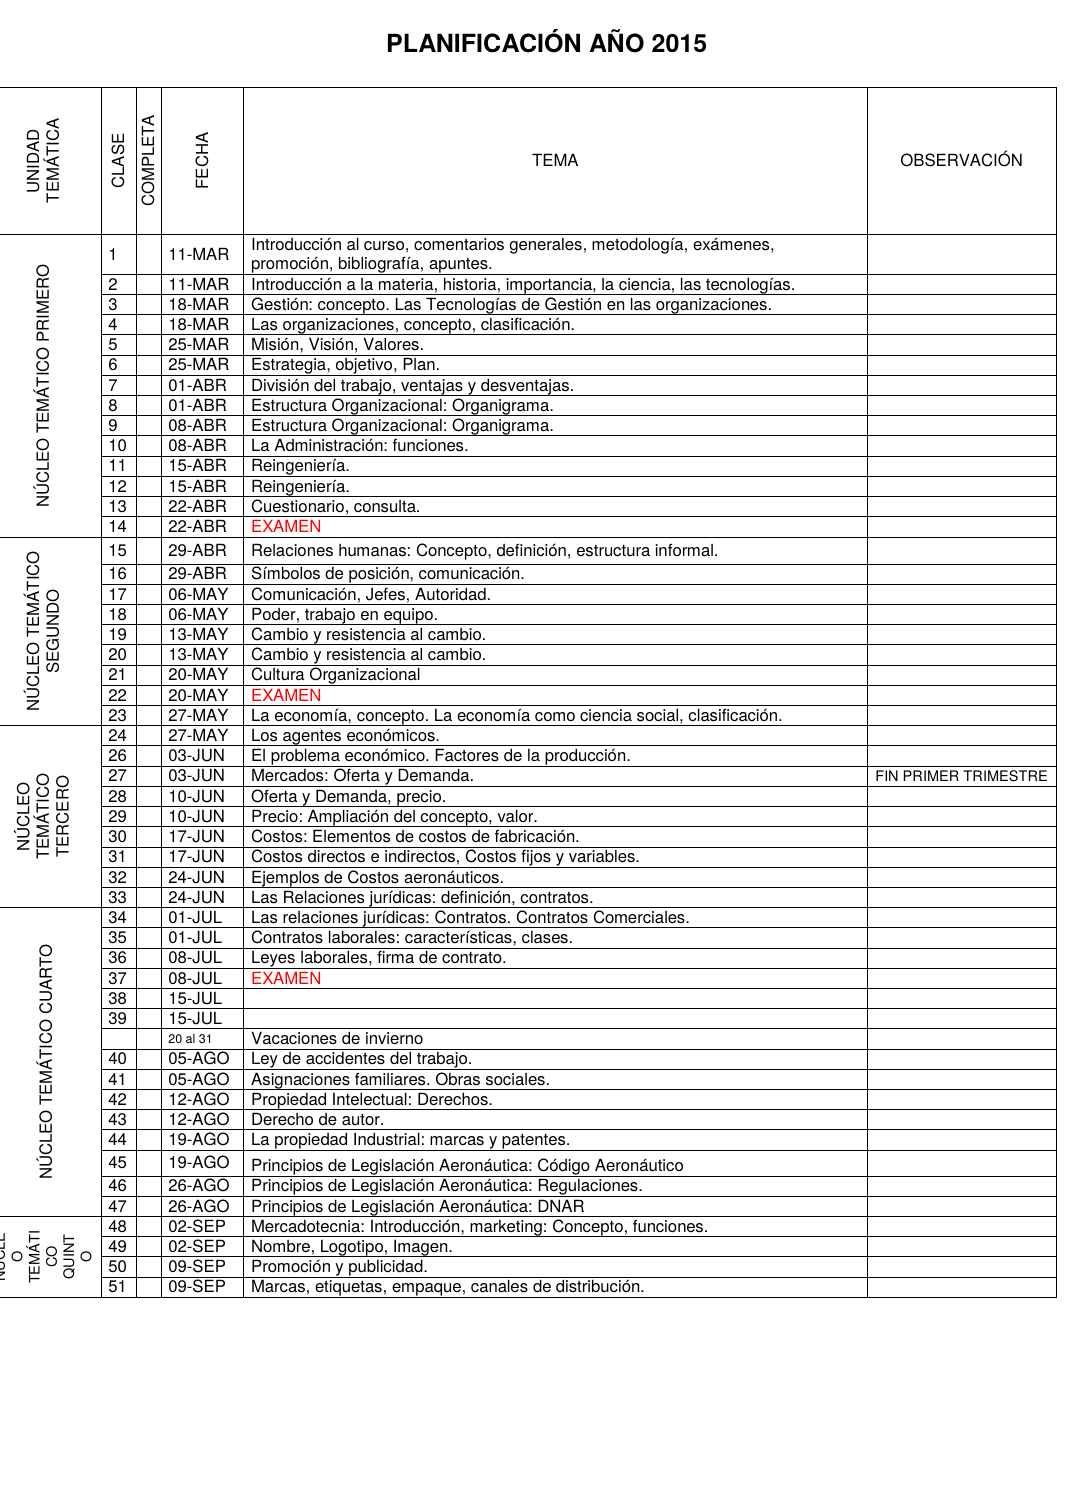
\includegraphics[width=1.00\linewidth]{figuras/fig_p004_01.png}
\end{center}

% ---- página 5 ----

\begin{center}
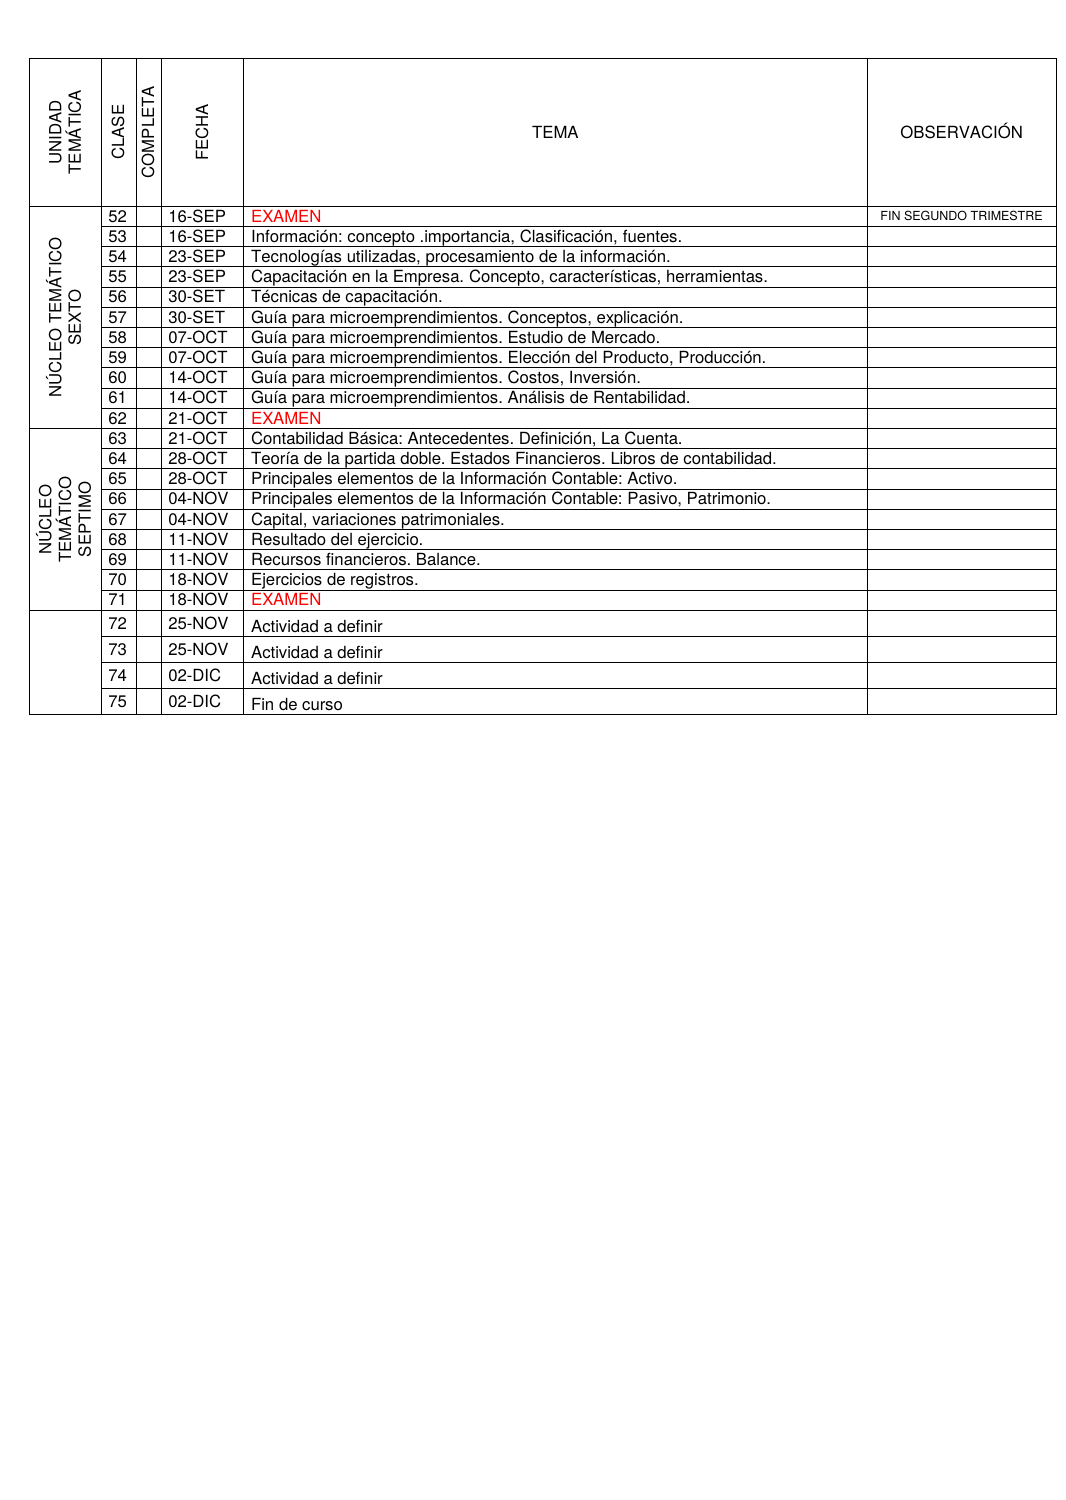
\includegraphics[width=1.00\linewidth]{figuras/fig_p005_02.png}
\end{center}

% ---- página 6 ----

\subsubsection*{CONTENIDOS DEL NÚCLEO TEMÁTICO PRIMERO}
Las Tecnologías de Gestión, concepto. Gestión: Concepto.

\section*{TECNOLOGÍAS DE GESTIÓN}
Comenzaremos el estudio de este curso definiendo el concepto contenido en el titulo de la materia.

Como las tecnologías se relacionan con las ciencia, en primer lugar nos preguntaremos ¿qué es lo que entendemos por ciencia?

LA CIENCIA La ciencia es un metodo para responder preguntas teoricas, se ocupa de describir hechos y relaciones entre fenomenos observables, intenta hacer predicciones con base al comportamiento regular de las cosas y encontrar sus conexiones con otras, de establecer teorias que organizan y dan sentido a estos hechos y relaciones. Para que algo sea considerado cientifico debe cumplir con un riguroso proceso de analisis, observacion y ensayos, denominado el metodo cientifico.

\subsubsection*{LA TECNOLOGÍA}
La tecnología, por otro lado, tiene que ver con herramientas, tecnicas y procedimientos para aplicar los descubrimientos de la ciencia.

Es decir que la ciencia intenta explicar el comportamiento de las cosas: Sus reglas, y la tecnología utiliza ese conocimiento para aplicarlo en forma practica proyectando, creando y construyendo cosas destinadas al uso y disfrute de los seres humanos, en muchos casos para una vida mejor.

Estamos rodeados de tecnologías en nuestra vida cotidiana, por ejemplo fue Kutta en 1902 el primero que se dedico al estudio cientifico del movimiento de objetos en un fluido. Estos conocimientos se aplicaron en la construccion de los primeros aeroplanos que comensaron a volar en 1903. Debieron pasa muchos años para que diversas tecnologías provenientes de diferentes areas de la ciencia confluyeran en los modernos vehiculos que hoy vuelan sobre nuestras cabezas.

\section*{GESTIÓN}

\begin{recuadro}
\textbf{Es el conjunto de actuaciones integradas para el logro de objetivos a largo, mediano y} \textbf{corto plazo, incluye la acción y el efecto de conducir las actividades de manera tal que se} \textbf{realicen diligencias que conduzcan al fin preestablecido de las organizaciones}\textit{.}
\end{recuadro}

La gestión es la acción principal de la administración, es el eslabón intermedio entre la planificación y los objetivos que se pretenden alcanzar. En general la gestión abarca los siguientes aspectos: Administrativos, gerenciales, de política de personal, marketing, relaciones humanas, jurídicas, económicas, de planificación, programación, orientación, evaluación, etc. La gestión tiende a promover el mejoramiento de la calidad, lo que implica una acción interdisciplinaria (varias ciencias aportan) que abarca aspectos económicos, políticos y sociales.


\begin{center}

\includegraphics[width=1.00\linewidth]{figuras/fig_p006_03.png}
\end{center}

% ---- página 7 ----

\subsubsection*{TECNOLOGÍAS DE GESTIÓN}
\section*{TECNOLOGÍAS + GESTIÓN}

\begin{center}
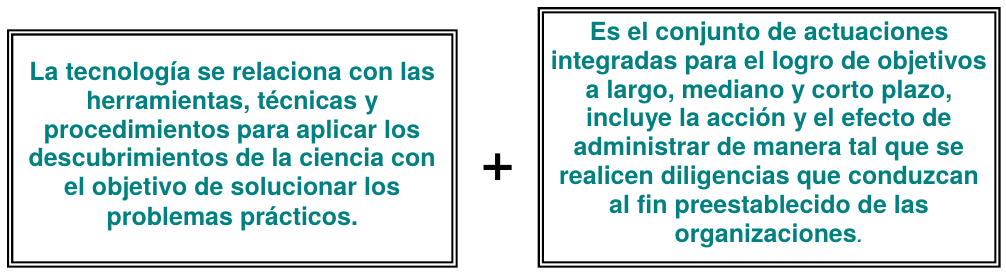
\includegraphics[width=1.00\linewidth]{figuras/fig_p007_04.png}
\end{center}

Si unimos los conceptos anteriores podemos definir las tecnologías de gestión de la siguiente forma:


\begin{recuadro}
\textbf{Es la aplicación práctica de los descubrimientos de la ciencia para asistir en la forma} \textbf{más eficiente a la conducción de las organizaciones para alcanzar sus objetivos.}
\end{recuadro}

En las organizaciones actuales convergen variadas tecnologías de distintos campos de las ciencias, centradas en el hombre y su entorno. Continuamente se agregan más, se actualizan, se modifican y se adaptan al complejo mundo en el que vivimos.

El siguiente esquema muestra algunas de las tecnologías que se aplican a las organizaciones actuales, algunas de ellas trataremos en este curso, y otras se trataran en otros cursos.


\begin{center}
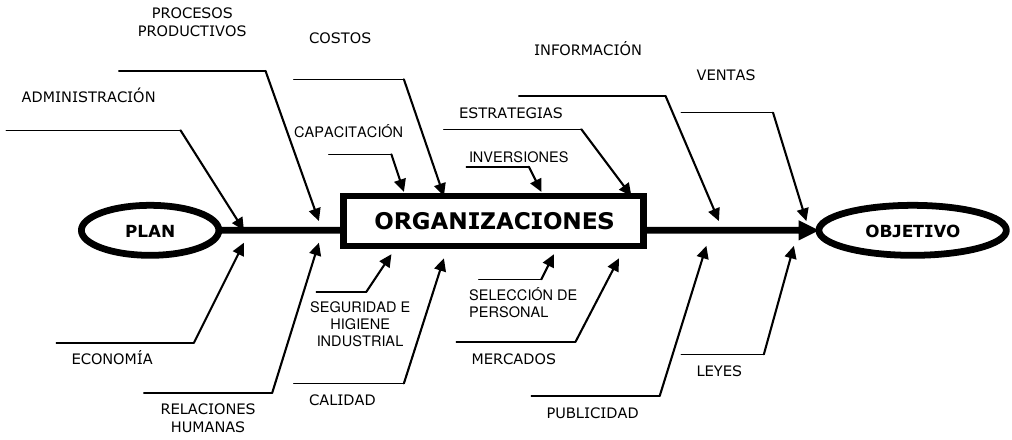
\includegraphics[width=1.00\linewidth]{figuras/fig_p007_05.png}
\end{center}

Las empresas están incorporando nuevos conceptos en su gestión: Internet y las nuevas tecnologías de información, la gestión de recursos humanos y del conocimiento, la globalización, el mayor poder en el cliente, el cambio constante, la gestión de la innovación, certificaciones de calidad, etc. Estos elementos que se van integrando en la gestión empresarial, obligan al modelo de negocio tradicional a evolucionar hacia nuevos modelos de gestión mejorando así la competitividad y los resultados empresariales.


% ---- página 8 ----

\subsubsection*{CONTENIDOS DEL NÚCLEO TEMÁTICO SEGUNDO}
Las organizaciones: Evolución, concepto, clasificación. La Empresa: Concepto, clasificación. Misión, Visión y Valores. Estrategias, Objetivos y Plan. División del trabajo. Estructura Organizacional: Organigrama. La Administración: Concepto, funciones, las organizaciones como sistemas. Reingeniería.

\section*{LAS ORGANIZACIONES}

\begin{recuadro}
\textbf{Las organizaciones son sistemas sociales constituidos por individuos (o grupos), con un} \textbf{objetivo en común, para cuyo logro desarrollan un sistema de actividades, utilizando} \textbf{recursos específicos y relacionándose con el entorno sobre el que influyen y por el que} \textbf{son influidos.}
\end{recuadro}

Estas organizaciones la forman personas físicas o jurídicas, que cooperan para satisfacer sus necesidades o deseos individuales o colectivos. La visión común sobre las organizaciones es de una estructura estática y rígida, sin embargo las organizaciones son dinámicas y en continua transformación, con un complicado sistema de relaciones humanas, adaptable a los cambios.

\subsubsection*{CLASIFICACIÓN DE LAS ORGANIZACIONES}
El hecho de clasificar objetos establece de por sí, el tener que determinar limites arbitrarios para diferenciar grupos de elementos que reúnen algún carácter común de otros grupos, pertenecientes al universo de elementos en estudio, con el objetivo de determinar un orden. El mismo grupo de elementos puede clasificarse de infinitas maneras dependiendo de la información sobre el grupo de elementos que se desee obtener con la clasificación.

La siguiente clasificación de las organizaciones es, por lo tanto, arbitraria. Otras clasificaciones


\begin{center}
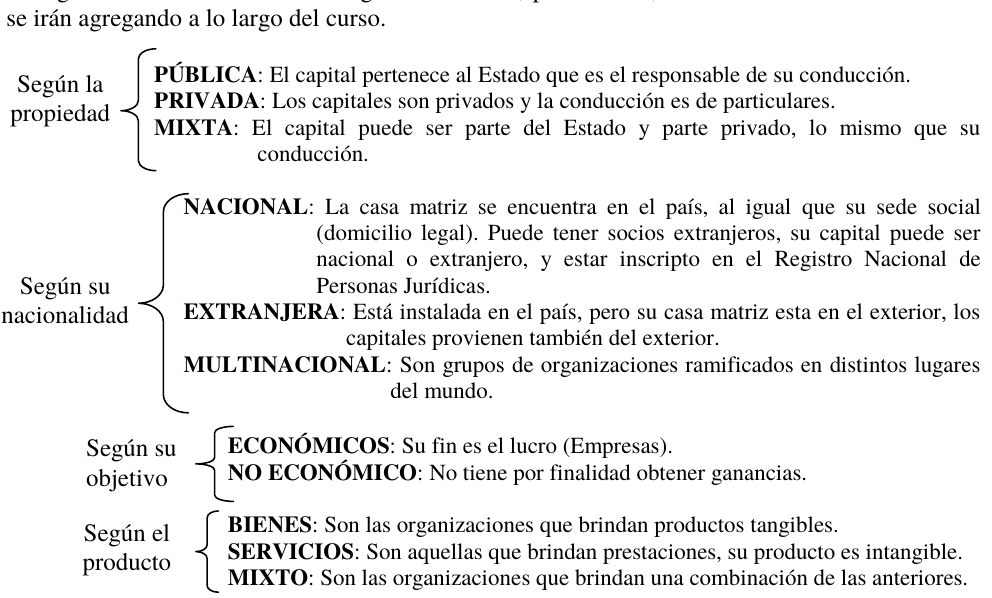
\includegraphics[width=1.00\linewidth]{figuras/fig_p008_06.png}
\end{center}

n

Estas son algunas de las formas en que se pueden clasificar las organizaciones, pero puede ser más extensa. Esta clasificación no es excluyente, es decir pueden ser organizaciones extranjeras


% ---- página 9 ----

con fines de lucro y proveedoras de servicios, los siguientes ejemplos ilustran sobre las gran diversidad de organizaciones: Organizaciones industriales (fábricas, metalúrgicas, cementeras), organizaciones comerciales (importadoras, empresas), organizaciones sindicales (mutuales, gremios), organizaciones educacionales (colegios, institutos, centros de capacitación, universidades), organizaciones financieras (bancos), organizaciones culturales (teatros), organizaciones deportivas (clubes), organizaciones sociales (consorcios, sociedades de fomento barrial), organizaciones agrícolas (rural), organizaciones profesionales (colegio de abogados, colegios de ingenieros), organizaciones ambientales (grupos ecológicos), organizaciones civiles (de seguridad vial, contra la droga, derechos humanos), organizaciones gubernamentales (ministerios, senado, municipalidades), organizaciones de beneficencia (hogares para menores).

\subsubsection*{EMPRESA}
Estas organizaciones comienzan su desarrollo durante la revolución industrial, modificándose gradualmente hasta la actualidad. En los principios el hombre dependía de la naturaleza y aprovechaba lo que la agricultura y la minería le brindaba, la forma de satisfacer las necesidades era el intercambio de productos (trueque) entre los distintos productores de una zona o región pequeña. La tierra y la mano de obra eran baratas (trabajada por esclavos). Durante los principios del desarrollo industrial el hombre comienza a modificar el medio dominando la naturaleza, aparecen los primeras tecnologías aplicados a la industria, la máquina de vapor que amplifica el trabajo del hombre y permite que los productos alcancen regiones distantes transportándose en ferrocarriles y barcos, la máquina de coser, telégrafo Morse, el cálculo infinitesimal que permitirá a las matemáticas servir de soporte a las ciencias físicas, aun la mano de obra era barata, ya no habían esclavos, pero los salarios eran bajos. A partir de la revolución industrial se produjo una profunda transformación en las formas de producción que dieron origen a una nueva institución contemporánea, una de las más importantes formas organizativas: La industria. En la época actual, con el aporte de la electrónica y los avances de las comunicaciones, le dan al hombre su independencia de la naturaleza y a las organizaciones el acceso fácil a la información y una adquisición de conocimientos menos costosa. En una época en que las innovaciones tecnológicas se suceden a ritmo vertiginoso, la manera de operar en las organizaciones debe ser adaptándose constantemente al medio. En la empresa esta es una nueva condición indispensable para no perder el ritmo de crecimiento. Después de la revolución industrial, el desarrollo de las organizaciones plantea un nuevo problema, el de su organización y dirección, para poder continuar su desarrollo y competir contra las demás empresas. Estos resultados solo se pueden obtener logrando una alta eficiencia.

\subsubsection*{DEFINICIÓN}
Son organizaciones comerciales constituidas por un conjunto de factores de producción (Recursos Naturales, Capital y Trabajo) que se aplican a la producción de bienes y servicios, partiendo de materias primas o de otros productos o insumos intermedios según la tecnología aplicada, dirigidos y controlados por el empresario, con el objetivo de obtener beneficios económicos consistente en la diferencia entre el precio de costo y el de venta, mediante la satisfacción de las necesidades del mercado donde actúa.

Una empresa, cuyo objeto es la producción, tendrá que elaborar sus productos para ofrecerlos al consumidor, ya sea directamente o haciendo uso de los distintos canales de distribución. Cualquier empresa que oferte sus productos en el mercado lo hará porque comprobó la necesidad de los mismos y anticipó los costos de los bienes que producen y sus ganancias. Esta necesidad se encontrará dada por la demanda. Las empresas que producen bienes destinados al consumo esperan la destrucción o consumición de los mismos y como consecuencia de ello la reposición.


% ---- página 10 ----

\subsubsection*{NACIMIENTO DE UNA EMPRESA}
La idea inicial de crear una empresa surge por diversas razones, que pueden ser: La posibilidad de un mercado interesante, el hallazgo de nuevas fuentes de riqueza, servicios nuevos, razones personales, deseo de independizarse, invertir un capital ahorrado u otras causas.

Todos estos motivos se unen a un proyecto empresarial que requiere un período hasta que madura la idea. El empresario deberá realizar distintos esquemas organizativos, conseguir los capitales necesarios los que pueden ser propios o ajenos permitiendo su puesta en funcionamiento.

El futuro empresario realizará la investigación del mercado, siendo este un elemento fundamental del proyecto de su empresa. Además, desarrollará los estudios necesarios para la puesta en marcha, determinará la forma jurídica y quienes serán sus colaboradores. A partir de este momento surge el lanzamiento de la empresa.

\subsubsection*{CLASIFICACIÓN}
De las múltiples clasificaciones que podemos encontrar de las empresas daremos solo algunos ejemplos.

Considerando la clasificación establecida por la Dirección de Asuntos Jurídicos del Ministerio de la Producción, en la Resolución Nº 24 del 15 de Febrero del 2001 de la ex Secretaria de la Pequeña y Mediana Empresa del Ministerio de Economía, tendremos la siguiente clasificación teniendo en cuenta el nivel máximo de las ventas totales anuales, consideradas en pesos argentinos, excluido el IVA, para los diferentes sectores de actividad de las empresas:


\begin{center}
\small
\begin{tabular}{|p{\dimexpr0.200\linewidth-2\tabcolsep\relax}|p{\dimexpr0.200\linewidth-2\tabcolsep\relax}|p{\dimexpr0.200\linewidth-2\tabcolsep\relax}|p{\dimexpr0.200\linewidth-2\tabcolsep\relax}|p{\dimexpr0.200\linewidth-2\tabcolsep\relax}|}
\hline
TAMAÑO/SECTOR & AGROPECUARIO & INDUSTRIA Y MINERÍA & COMERCIO & SERVICIOS \\ \hline
MICRO EMPRESA & \$ 270.000 & \$ 9.000.000 & \$ 1.800.000 & \$ 450.000 \\ \hline
PEQUEÑA EMPRESA & \$ 1.800.000 & \$ 5.400.000 & \$ 10.800.000 & \$ 3.240.000 \\ \hline
MEDIANA EMPRESA & \$ 10.800.000 & \$ 43.200.000 & \$ 86.400.000 & \$ 21.600.000 \\ \hline
\end{tabular}
\end{center}

También podemos clasificarlas según sean:

Empresas Mayoristas: Son aquellas que adquieren los productos para su venta a otras empresas comprendidas en la cadena de distribución para llegar a los minoristas.

Empresa Minoristas: Son las que venden directamente al consumidor final.

Teniendo en cuenta su tamaño las podemos clasificar en:

MICROEMPRENDIMIENTOS: Son las empresas que tienen menos de cinco empleados. PyMEs: Son las pequeñas y medianas empresas, en nuestro país y según el sector están entre 100 y 300 empleados, y GRANDES ORGANIZACIONES: Todas aquellas que superan los límites de la PyMEs.


% ---- página 11 ----

\section*{VISIÓN, MISIÓN Y VALORES}
Cuando una organización ha definido su Visión, su Misión y sus Valores, tiene una tarjeta de presentación que refleja su identidad: \textbf{\textit{Lo que la Empresa es o quiere ser}}. Pero si no tiene, o no usa las herramientas para convertir en realidad su Visión y su Misión, éstas se quedan solo en el terreno de las buenas intenciones. Desdoblar la complejidad de la Visión y la Misión, en Áreas Clave de Resultados, Objetivos concretos, Estrategias específicas e Indicadores de actuación, es el primer paso para poner en movimiento a toda la Organización hacia el cumplimiento de su Misión y el logro de su Visión.

Las empresas que deciden crear y proyectar su propio futuro inician con la preparación y formulación del Plan Estratégico de la Organización, que contesta algunas preguntas básicas:

\subsection*{¿Quiénes somos y cuál es nuestro papel?}
\subsection*{¿Dónde estamos hoy y dónde queremos estar mañana?}
\subsection*{¿Cómo lo vamos a lograr?}
\subsubsection*{VISIÓN}
A los fundadores, creadores de empresas – hoy grandes empresas – al comienzo, se le llamó “visionarios” o “soñadores”, posiblemente con el matiz de “ilusos” o “locos”, pero cuando se les pregunta a estos visionarios y soñadores ¿cuál fue la razón de su éxito?, todos, sin excepción, contestan que \textit{“sabían lo que querían”, }y con esto han definido lo que es VISIÓN: “Saber lo que queremos ser”.

\subsubsection*{FORMULAR LA DECLARACIÓN DE LA VISIÓN}
Quien va a liderar el proceso de construcción y desarrollo de una VISIÓN debe comenzar con la formulación de una primera declaración de la Visión, en términos claros, precisos, concisos e impactantes. Este paso es fundamental para la construcción del modelo de visión. Cuando la VISIÓN está bien formulada, comunicada y compartida, se convierte en el norte magnético que alinea, orienta y atrae todas las energías de la gente en una sola dirección: "el logro de la Visión". La primera declaración debe reflejar la aspiración más alta, como meta final, aunque, a primera vista, parezca inalcanzable: "\textit{Ser el mejor en... }", "\textit{ser la más grande de...}", "\textit{ser los primeros} \textit{en...}", etc., siempre en términos positivos y optimistas. La declaración de la visión debe proporcionar inspiración, motivación y energía a la Organización, a las unidades funcionales y a las personas. Por ejemplo: \textbf{\textit{“Ser la línea de transporte aéreo de mayor seguridad y}} \textbf{\textit{cumplimiento en los países donde opera” }}o \textbf{\textit{“Queremos ser la mejor organización de servicio}} \textbf{\textit{en el mundo” (IBM). “Llegamos a donde la gente no llega” (FEDEX).}}

Sin embargo, las visiones tipo "slogan", impuestas desde lo alto, no funcionan. La gente las percibe como "\textit{ésa es la visión de los de arriba, pero no es la mía}" y no se comprometen con ella. Como afirma Peter Senge: "\textit{Muchos líderes tienen visiones personales que nunca se} \textit{traducen en visiones compartidas que galvanicen a una organización. Hemos estado careciendo} \textit{de una disciplina para traducir la visión individual en una visión compartida"}.

\begin{itemize}
  \item La Visión es una imagen del futuro deseado que buscamos crear.
  \item La declaración de una Visión captura, en palabras, las ideas de las personas que conforman
\end{itemize}
una organización acerca de qué se quiere lograr y dónde se quiere estar en el futuro.

\begin{itemize}
  \item Debe ser suficientemente amplia, que rete a toda la Organización, y suficientemente
\end{itemize}
detallada, que señale el camino a todos.


% ---- página 12 ----

\subsubsection*{MISIÓN}
Todo lo que existe en el universo tiene una finalidad, un propósito, una razón de ser, un motivo para existir. A eso se le llama MISIÓN. Su definición responde a la pregunta ¿por qué y para qué estamos aquí?. Aunque desde sus orígenes la palabra “misión” ha tenido connotaciones religiosas o militares, inmediatas –“\textit{Nuestra misión es tomar la colina (¡o morir en el intento!})”

– su sentido de “propósito” y “finalidad” se mantiene en el contexto actual. De hecho, toda empresa y toda organización humana tiene una finalidad, tácita o explícita, sea que la conozcan todos o no. Aunque, la verdad es que muchas empresas, como muchas personas, nacen y mueren sin tener claridad de cuál fue el propósito de su vida.

\subsubsection*{DIFINIR LA MISIÓN}
La importancia de definir con claridad y exactitud la misión, en el mundo de los negocios, surge en la década de los 70, con el auge de la planeación estratégica, como la mejor (¿y única?) herramienta de supervivencia y crecimiento, en mercados que se abrían a la competencia mundial, cada vez más feroz y agresiva, en la cual, se triunfa o se muere. No hay alternativa. En el proceso de formulación del futuro, la “misión compartida” tiene importancia esencial. Esta se desprende necesariamente de la “visión”. Si la visión nos dice lo que queremos ser, la misión nos indica lo que debemos hacer para lograrlo.

La declaración de la MISIÓN es la respuesta a las preguntas: ¿En qué negocio estamos?, ¿Por qué estamos en esto?, ¿Para qué hacemos lo que hacemos?, ¿Cuál es nuestro propósito más importante como Empresa, como Área Funcional, como Trabajadores?, ¿Cuál es nuestra razón de ser?, ¿A qué estamos contribuyendo?

\begin{itemize}
  \item La misión puede ser definida como la razón de ser o existir.
  \item Es la contribución única o distintiva que cada persona y cada grupo de la Empresa debe hacer
\end{itemize}
para la consecución de los resultados totales de la Organización, identificando: A qué contribuye; el sistema usuario; la naturaleza de las necesidades de éste y cómo contribuye.

Un ejemplo: \textit{“Nuestra misión es satisfacer las necesidades y expectativas del viajero frecuente y} \textit{del turista con oportuno y excelente servicio, dentro de los parámetros de la más alta seguridad.} \textit{Será la tarea y compromiso total de todos los miembros de AEROSUR, para lograr así la} \textit{oportuna y adecuada retribución a sus empleados, a sus accionistas y a la sociedad en general”.}

\subsubsection*{VALORES}
Los valores son los principios fundamentales, los cimientos, sobre los cuales se construye la casa. La visión es lo que queremos construir y los valores son las bases. Los valores no están en la organización, están en la gente. Los valores que tiene la gente son los que conforman la “Cultura de la Empresa” y son los que imperan en el clima laboral. La visión, misión, los objetivos y las estrategias, deben ser compartidos y hay que alinearlos. Los valores impuestos desde arriba y divulgados como el credo organizacional no guían ni mueven a nadie, si no son compartidos por la gente.

\subsubsection*{DEFINIR LOS VALORES QUE CONFORMAN LA CULTURA}
Cuando los valores constituyen la parte fundamental del proyecto de visión compartida, y se exponen a la vista de todos, se convierten en la guía de la conducta de la gente y que le ayuda a moverse en la dirección que le marcan la visión y la misión.

\begin{itemize}
  \item Son guías de pensamiento y acción que enmarcan y determinan los comportamientos de las
\end{itemize}
personas.


% ---- página 13 ----

\begin{itemize}
  \item Son las creencias, actitudes, formas de pensar e ideologías que dirigen la forma de hacer
\end{itemize}
nuestro trabajo y de interactuar con los demás, y que crean la “cultura organizacional”. Un conjunto de valores rectores deberá incluir: Pautas de conducta recíproca, apreciación de la clientela, relaciones con la comunidad y los límites que voluntariamente nos imponemos.

\begin{itemize}
  \item Los Valores se definen preguntándonos y contestándonos: ¿Cuáles son los valores
\end{itemize}
institucionales que requieren la nueva Visión y Misión de la Compañía? ¿Cuáles valores nos generaran ventajas competitivas? ¿Cómo queremos que se sientan los clientes, los empleados, los proveedores y los accionistas en relación con la Empresa?

\begin{itemize}
  \item Las siguientes preguntas son especialmente útiles para que el grupo clarifique y defina sus
\end{itemize}
valores fundamentales: ¿Cómo tratamos a nuestros clientes?; ¿cómo tratamos a nuestros colaboradores?; ¿qué queremos decir con conducta ética?; ¿cuáles valores fundamentales nos importan más que las ganancias?; ¿qué conductas reflejarían estos valores?; ¿cómo queremos tratarnos mutuamente en el trabajo?; ¿qué ofrecemos a nuestros colaboradores por su esfuerzo laboral?; ¿qué actitudes y comportamientos de nuestros colaboradores queremos recompensar?

\section*{LA ESTRATEGIA Y EL OBJETIVO}
\subsubsection*{INTRODUCCIÓN}
La estrategia nació en el campo militar como la forma de ganar la guerra. En el mundo de los negocios la estrategia conserva idéntico sentido: La guerra de las pizzas, la guerra de las cadenas de televisión. En nuestro contexto la estrategia o estrategias responden al COMO lograr lo que ya hemos formulado: Visión y Misión. Su definición y formulación son solo deseos. La estrategia es el proceso y la acción que los realiza.

Los objetivos se concretan cuando se logran los resultados esperados. Los objetivos son el “resultado de...” Los objetivos bien formulados nos indican el punto exacto de llegada. La estrategia es el plan de vuelo que debe considerar los recursos que tenemos, cuáles son nuestros puntos fuertes (valores) y cuáles los débiles (disvalores). En qué somos buenos y en qué no lo somos. Cuáles son las condiciones del medio ambiente (mercado y competencia). Qué condiciones están a nuestro favor y cuáles son los peligros. En la adecuada combinación y uso de estas variables está la clave para diseñar y ejecutar las estrategias más adecuadas para el logro de objetivos y metas.

Los objetivos están en función de las estrategias. Alguien dijo que \textit{“no existen objetivos} \textit{inalcanzables, sino estrategias equivocadas”. }En la medida en que las estrategias estén bien diseñadas y puestas en marcha, generalmente los objetivos se alcanzan y, con frecuencia, se superan.

Las Estrategias se construyen preguntando y contestando:

\begin{itemize}
  \item ¿Cuáles son los objetivos que queremos lograr?
  \item ¿Cómo podemos lograrlos, al menor costo y con la mayor efectividad?
  \item ¿Cuáles son nuestras áreas más fuertes en conocimientos, habilidades y recursos?
  \item ¿Cuáles son nuestras áreas más débiles?
  \item ¿Cuáles son las condiciones de mercado que más nos favorecen?
  \item ¿Cuáles son los mayores peligros que nos amenazan?
\end{itemize}

% ---- página 14 ----

\subsubsection*{CONCEPTO}
Normalmente una organización está en una situación “A“, que se conoce por un diagnostico, esta empresa desea llegar en un determinado plazo (por ejemplo 3 años) a la situación “B” (objetivo) en función de las oportunidades que el medio presenta.

Para establecer el punto “B” la empresa toma en cuenta, como orientación, su destino final o su aspiración final Z (visión) .Para pasar de “A” a “B” pueden existir varios caminos que habrá que formular y evaluar.

A estos caminos, rumbos o vías para alcanzar el objetivo se los llama ESTRATEGIAS. Elegido uno de los caminos, se ha determinado la estrategia para alcanzar el objetivo, es necesario precisar entonces las metas parciales entre A y B (plan). Al analizar los caminos alternativos algunos quedaran eliminados si no se quieren usar. La elaboración de la estrategia es una función de la ADMINISTRACIÓN, GERENCIA o PRESIDENCIA (máximo nivel jerárquico). Este sencillo ejemplo puede aclararnos el concepto: Juan está en una situación (A) pobre y quiere llegar a ser rico (B) porque esto le permitirá ser feliz (Z). Para pasar de pobre a rico tiene varias alternativas (estrategias): Trabajar, ganarse la lotería, especular en la bolsa, casarse con una mujer rica, robar un banco, vender droga, etc. Por razones religiosas, legales y morales decide no robar ni hacer transacciones ilícitas (de los caminos posibles descarta aquellos que no quiere transitar, fija una política), evalúa las distintas alternativas, considera el riesgo de cada una de ellas y decide intentar hacerse rico abriendo un taller de reparaciones de aeronaves (estrategia). Se fija entonces metas parciales: Crear una sociedad en 3 meses, abrir el taller en 9 meses,


\begin{center}
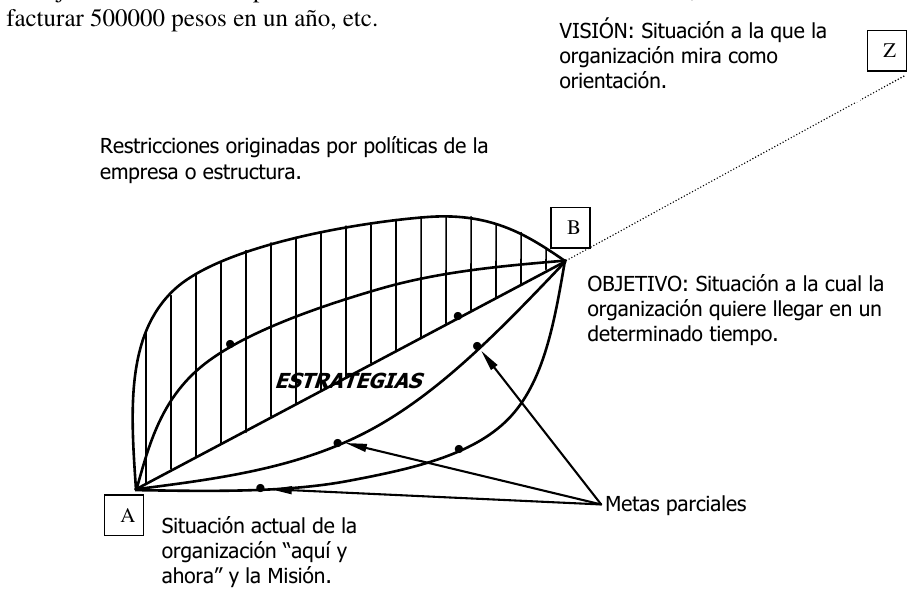
\includegraphics[width=0.94\linewidth]{figuras/fig_p014_07.png}
\end{center}

Como su capital es limitado tiene algunas restricciones. La decisión está influenciada por sus conocimientos de aeronáutica y porque un familiar le presta las instalaciones para armar su taller (valores y recursos). La ubicación del taller le permitirá brindar sus servicios a todos los poseedores de aeronaves pequeñas de la zona norte. (Misión).


% ---- página 15 ----

\section*{PLANIFICACIÓN Y PLAN}
La planificación es la traducción de un conjunto de actividades y operaciones temporizadas establecidas previamente, en una guía de procedimientos escrito llamada plan. Es un esfuerzo de resolución de problemas y toma de decisiones que involucra pensar en el futuro, decidir sobre el futuro deseado (visión) y las acciones (gestión) para alcanzarlos, y establecer las metas parciales para alcanzar el objetivo establecido.

Esta también una de las funciones de la administración y está íntimamente relacionada con las demás: Organización, control y conducción.

Una vez establecida la visión, misión y el objetivo, y determinada la estrategia para alcanzar el objetivo, surge el plan general (ver las cualidades que debe reunir un plan en las funciones de la administración), del cual surgirán los planes parciales que cada área de la organización deberán gestionar para aportar a la concreción del plan general. Del plan general surgirán los presupuestos de recursos necesarios para llevarlo a término.


\begin{center}
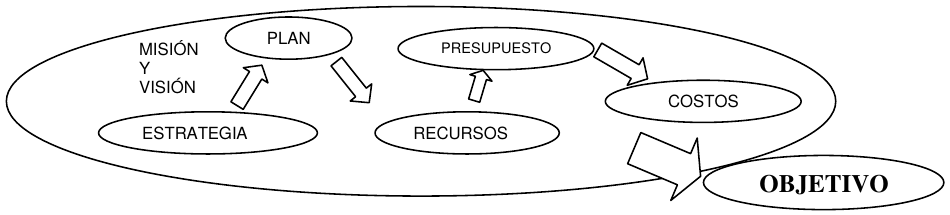
\includegraphics[width=0.97\linewidth]{figuras/fig_p015_08.png}
\end{center}

Lectura recomendada

\subsubsection*{LAS ORGANIZACIONES INTELIGENTES}
Los ingenieros dicen que se ha inventado una idea nueva cuando se demuestra que funciona en el laboratorio. La idea se transforma en innovación sólo cuando se puede reproducir sin contratiempos en gran escala y a costos prácticos.

En 1903, la frágil aeronave de Wilbur y Orville Wright demostró que era posible volar con máquinas de motor. Así se inventó el aeroplano, pero pasaron más de treinta años hasta que la aviación comercial pudiera servir al público en general. Siguiendo este ejemplo, podemos decir que las organizaciones inteligentes ya se han \textit{inventado}, pero aún no se han \textit{innovado}. En ingeniería, para que una idea pase de la invención a la innovación, confluyen diversas tecnologías de componentes. Estos componentes, nacidos de desarrollos aislados en diversas áreas de la investigación, configuran gradualmente un conjunto de tecnologías que son fundamentales para el mutuo éxito. Mientras no se forme ese conjunto, la idea, aunque posible en el laboratorio, no alcanza su potencial en la práctica.

En 1935, el DC-3 de McDonnell Douglas inauguró la era del viaje aéreo comercial, ya que fue el primer avión que se mantenía no sólo aerodinámicamente sino también económicamente. Antes habían fracasado muchísimos experimentos con vuelos comerciales. Como los primeros experimentos con las organizaciones inteligentes, los primeros aviones no eran confiables ni tenían un costo efectivo en la escala apropiada. El DC-3, por primera vez, eslabonó cinco tecnologías de componentes decisivas para formar un conjunto de éxito. Se trataba de la hélice de paso variable, el tren de aterrizaje retráctil, un tipo de construcción ligera llamada monocasco, el motor radial enfriado por aire y los alerones. El DC-3 necesitaba las cinco: Cuatro no eran suficientes. Un año antes se había introducido el Boeing 247, que incluía todo esto salvo los alerones. La falta de alerones volvía al Boeing inestable durante el despegue y el aterrizaje y los ingenieros tuvieron que reducir el tamaño del motor.

En la actualidad, nuevas tecnologías de componentes convergen para innovar las organizaciones inteligentes. Aunque se desarrollaron por separado, cada cual resulta decisiva para el éxito de las demás, tal como ocurre con cualquier conjunto. Cada una de ellas brinda una dimensión vital para la construcción de organizaciones con auténtica capacidad de aprendizaje, aptas para perfeccionar continuamente su habilidad y alcanzar sus mayores aspiraciones.


% ---- página 16 ----

\textit{Este artículo forma parte de la serie de contenidos dedicados al concepto: Organizaciones Scouts abiertas al} \textit{aprendizaje. Para su mejor comprensión, recomendamos leer los fascículos editados por la Red de Desarrollo} \textit{Institucional.}


\begin{recuadro}
\subsubsection*{FEDERICO TAYLOR (1856-1915)}
Hoy se lo reconoce universalmente como el fundador de la ciencia de la organización del trabajo, dedico toda su vida a estudiar el trabajo del hombre aplicando el racionalismo científico. Una de las recomendaciones formuladas por Taylor es la siguiente: Distribuir la responsabilidad y el trabajo de acuerdo a las capacidades de los trabajadores.
\end{recuadro}

\subsubsection*{CUESTIONARIO 1}
1. Definir que son las organizaciones y quienes pueden integrarlas.

2. ¿Qué tecnologías utilizan las organizaciones?

3. ¿Qué tecnologías utilizan las organizaciones para publicitar sus productos?

4. ¿La conducción de las organizaciones científicamente sugiere la toma de decisiones racionales o emocionales?

5. Definir gestión.

6. ¿Las organizaciones son cambiantes? Justificar la respuesta.

7. Mencione 3 ejemplos de organizaciones, según la clasificación dada.

8. ¿Por qué la gestión en las organizaciones es una acción interdisciplinaria?

9. Mencionar un ejemplo de Misión, Visión y Objetivo de una organización educativa.

10. Clasificar las siguientes ideas según sean valores (V), disvalores (D) o recursos (R):


\begin{center}
\small
\begin{tabular}{|p{\dimexpr0.249\linewidth-2\tabcolsep\relax}|p{\dimexpr0.249\linewidth-2\tabcolsep\relax}|p{\dimexpr0.249\linewidth-2\tabcolsep\relax}|p{\dimexpr0.249\linewidth-2\tabcolsep\relax}|}
\hline
Certificación ISO & Capacitación del personal & Estructura edilicia & Maquinarias \\ \hline
Individualismo & honestidad & motivación & falta de interés por los demás \\ \hline
crecimiento personal basado en el mérito & empleo como subsidio & desmotivación & confianza \\ \hline
falta de liderazgo & trabajo en equipo & renombre & marcas y patentes \\ \hline
corrupción & valoración solo de la antigüedad y conocimientos operativos & organización fragmentada & concepto de usuario y público en lugar de clientes \\ \hline
responsabilidad & energía, mano de obra & conocimiento & tiempo \\ \hline
conflictos de intereses & vehículos, materiales, muebles, herramientas & organización introvertida & personería jurídica \\ \hline
\end{tabular}
\end{center}

11. ¿Se le ocurre otra forma de clasificar a las organizaciones?

12. ¿Qué es una estrategia?

13. ¿Es válido definir a la estrategia como: El curso de acción para alcanzar el objetivo?

14. ¿Quién tiene la tarea de elaborar una estrategia?

15. ¿El personal de una empresa debe conocer la estrategia planeada? ¿Por qué?

16. ¿Cuándo una estrategia puede cambiar?

17. Debatir sobre lo siguiente: Aceptación del riesgo: Como el futuro es incierto toda decisión estratégica involucra un riesgo importante. Sin embargo, el peor de los riesgos es no hacer nada, quedar paralizado mientras se analiza y analiza.

18. Un plan es una guía de procedimientos escritos que surge de la estrategia adoptada por la organización para alcanzar los objetivos propuestos. ¿Quién tiene la función de confeccionarlo?


% ---- página 17 ----

\subsubsection*{DIVISIÓN DEL TRABAJO}
En las pequeñas organizaciones todas las tareas que se deben realizar en la organización se encuentran a cargo del dueño y algún colaborador o familiar, pero cuando las organizaciones comienzan a desarrollarse y crecer se tornan más complejas y las tareas se encuentran distribuidas entre mayor cantidad de personal, surgen la necesidad de definir las responsabilidades y funciones de las personas o grupos que realizan tareas determinadas. La división del trabajo consiste en asignar las diferentes tareas que se deben realizar en las organizaciones a grupos o personas acorde a su aptitud y capacidad.

Esta división de las tareas dará origen a la estructura organizacional que veremos más adelante, en el cual se representa esta división de tareas gráficamente por el \textbf{organigrama}, en ella se ve como se dividen las tareas asignadas a diferentes personas o grupos.

\subsubsection*{LA ORGANIZACIÓN Y SUS ÓRGANOS}
Si dividiéramos las tareas que se deben ejecutar en todas las organizaciones según su afinidad, obtendríamos un conjunto definido de tareas a realizar en cada área, por ejemplo el área contable tendría a cargo las tareas de registrar los movimientos de entrada y salida de dinero, balance general, inventarios, manejo de las cuentas bancarias, etc., el área de personal tendría las tareas de registrar las inasistencias y llegadas tarde del personal, registro de antecedentes y sanciones disciplinarias en los legajos, elaboración de los contratos laborales, determinación de las licencias de vacaciones, actualizar la información sobre salarios familiares, etc. En el área de comercialización tendremos las tareas de publicidad, relaciones públicas, encuestas. En el área de producción las tareas se dividen en tantas partes como se requiera según las operaciones a realizar, y de esta forma en todas las organizaciones habrá grupos que realicen las diferentes tareas.

Cuando las tareas a realizar, ordenadas por áreas, son designadas a un grupo de personas, estos grupos de personas forman los órganos ejecutores de esas tareas, de esta forma se tendría un órgano ejecutor de las tareas contables, un órgano ejecutor de las tareas de personal, un órgano ejecutor de las tareas administrativas, un órgano ejecutor de las tareas legales, etc.

El siguiente gráfico representaría la división de las tareas, según los órganos, en una


\begin{center}
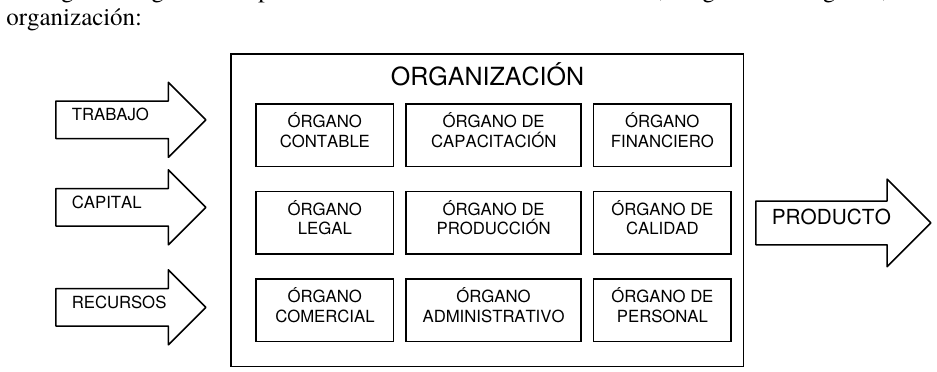
\includegraphics[width=0.96\linewidth]{figuras/fig_p017_09.png}
\end{center}

La organización recibe trabajo, capital y recursos del entorno para elaborar su producto, la organización los distribuye a los diferentes órganos para que realicen sus tareas específicas, el resultado de estas tareas será el producto que brinde cada órgano a la organización. Si analizáramos gráficamente uno de estos órganos, por ejemplo la administración, el producto que


% ---- página 18 ----

brinda sería el planeamiento, la organización, el mando, la coordinación y el control y vigilancia, es decir las funciones que tienen a cargo que veremos más adelante.


\begin{center}
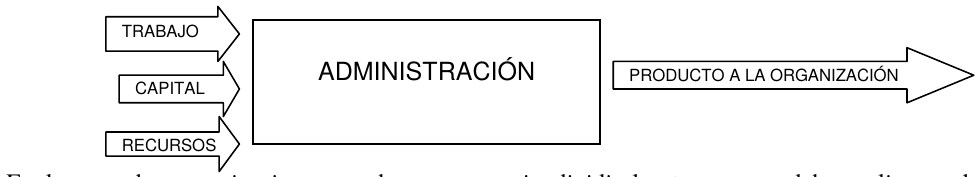
\includegraphics[width=1.00\linewidth]{figuras/fig_p018_10.png}
\end{center}

En las grandes organizaciones puede ser necesario dividir las tareas que debe realizar cada órgano y asignarla a grupos determinados de personas, que también recibirán trabajo, capital y recursos de la organización para brindar su producto a la organización, que será el resultado de la tarea que se le asignó. Siguiendo con el ejemplo anterior tendríamos:


\begin{center}
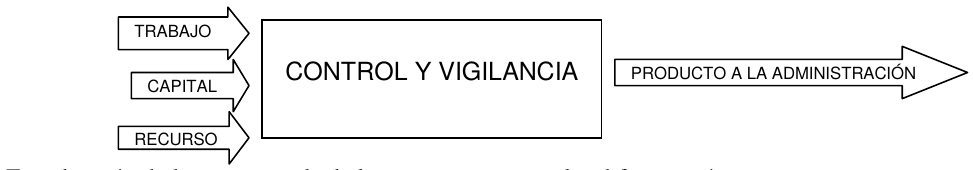
\includegraphics[width=0.99\linewidth]{figuras/fig_p018_11.png}
\end{center}

Esta división de las tareas se da de la misma manera en las diferentes áreas.

En el cuadro siguiente se mencionan algunas de las diferentes tareas que se realizan en una organización y como estas se agrupan según el área afín.


\begin{center}
\small
\begin{tabular}{|p{\dimexpr0.316\linewidth-2\tabcolsep\relax}|p{\dimexpr0.348\linewidth-2\tabcolsep\relax}|p{\dimexpr0.336\linewidth-2\tabcolsep\relax}|}
\hline
CONTABLES \newline \textbullet~BALANCES \newline \textbullet~REGISTROS CONTABLES \newline \textbullet~PAGO DE IMPUESTOS \newline \textbullet~ELABORACIÓN DE PRESUPUESTOS \newline \textbullet~LIQUIDACIÓN DE SUELDOS \newline \textbullet~CONTROL DE GASTOS \newline \textbullet~COMPRAS \newline \textbullet~CONTROL DE COSTOS \newline \textbullet~ETC. & PRODUCCIÓN \newline \textbullet~ABASTECIMIENTO DEL MATERIAL \newline \textbullet~ELABORACIÓN DEL PRODUCTO \newline \textbullet~DEPÓSITOS \newline \textbullet~ALMACENES \newline \textbullet~ENVASADO \newline \textbullet~TRANSPORTE \newline \textbullet~ETC. & ADMINISTRACIÓN \newline \textbullet~ELABORACIÓN DEL PLAN \newline \textbullet~DESIGNACIÓN DE JERARQUÍAS \newline \textbullet~DETERMINACIÓN DE ESTRATEGIAS \newline \textbullet~CONTROL DEL PLAN \newline \textbullet~ORGANIZACIÓN \newline \textbullet~ASIGNACIÓN DE RECURSOS \newline \textbullet~COORDINACIÓN \newline \textbullet~ETC. \\ \hline
FINANCIERAS \newline \textbullet~BÚSQUEDA DE INVERSIÓN \newline \textbullet~ASIGNACIÓN DE LAS GANANCIAS \newline \textbullet~ASIGNACIÓN DE RECURSOS \newline \textbullet~BÚSQUEDA DE SOCIOS \newline \textbullet~POLÍTICAS FINANCIERAS \newline \textbullet~ETC. & COMERCIALES \newline \textbullet~BÚSQUEDA DE MERCADOS \newline \textbullet~BÚSQUEDA DE CLIENTES \newline \textbullet~PUBLICIDAD \newline \textbullet~VENTAS \newline \textbullet~DISTRIBUCIÓN DE PRODUCTOS \newline \textbullet~RELACIONES PÚBLICAS \newline \textbullet~ETC. & GENERALES \newline \textbullet~MANTENIMIENTO EDILICIO \newline \textbullet~MANTENIMIENTO DE VEHÍCULOS \newline \textbullet~PROVISIÓN DE INSUMOS \newline \textbullet~HIGIENE \newline \textbullet~SEGURIDAD \newline \textbullet~MANTENIMIENTO DE MAQUINARIAS Y EQUIPOS \newline \textbullet~ETC. \\ \hline
LEGALES \newline \textbullet~CONTRATOS \newline \textbullet~ASESORAMIENTOS \newline \textbullet~JUICIOS \newline \textbullet~DESPIDOS \newline \textbullet~ETC. & DE SOPORTE \newline \textbullet~INFORMÁTICA \newline \textbullet~ARCHIVOS \newline \textbullet~REGISTROS \newline \textbullet~ASISTENCIA MÉDICA \newline \textbullet~SEGUROS \newline \textbullet~ETC. & PERSONAL \newline \textbullet~SELECCIÓN \newline \textbullet~CONTRATACIÓN \newline \textbullet~CAPACITACIÓN \newline \textbullet~CONTROL DE AUSENTISMO \newline \textbullet~REGISTROS \newline \textbullet~CATEGORIZACIÓN \newline \textbullet~ASIGNACIONES \newline \textbullet~ETC. \\ \hline
\end{tabular}
\end{center}

% ---- página 19 ----

Una de las áreas más populares asociada a la actividad de los Técnicos Aeronáuticos en las compañías aéreas es la de Producción en el cual, dependiendo de la organización, este órgano tendrá la función de mantener el material aeronáutico en condiciones para prestar los servicios que la organización brinda. En las organizaciones de reparaciones aeronáuticas, por ejemplo, observamos como se reparten a diferentes grupos especializados las tareas de mantenimiento: El personal especializados en equipos electrónicos de abordo, son los encargados de las reparaciones de los equipos de aviónica.

Por último podemos mencionar que los órganos pertenecientes a una organización no se encuentran necesariamente en el mismo lugar físico, por ejemplo AEROLÍNEAS ARGENTINAS tiene su órgano de administración en la calle Buchard en Capital Federal, su órgano de ventas en la calle Perú también de Capital, su órgano de capacitación en Ezeiza y su órgano de producción en Ezeiza y Aeroparque. Otras organizaciones pueden tener su órgano de administración en el extranjero.

\subsubsection*{VENTAJAS Y DESVENTAJAS DE LA DIVISIÓN DEL TRABAJO}

\begin{center}
\small
\begin{tabular}{|p{\dimexpr0.517\linewidth-2\tabcolsep\relax}|p{\dimexpr0.483\linewidth-2\tabcolsep\relax}|}
\hline
VENTAJAS & DESVENTAJAS \\ \hline
\textbullet~Permite asignar las tareas a cada trabajador o grupo según sus condiciones en las actividades en que puede rendir mejor. \newline \textbullet~Permite al trabajador o grupo desarrollar mayor destreza, lo que mejora la producción y calidad. \newline \textbullet~Ahorra el tiempo que normalmente se desperdicia al pasar a un trabajador o grupo de una tarea a otra. \newline \textbullet~Permite al trabajador o grupo profundizar en la tarea y les da la oportunidad de descubrir métodos para perfeccionarla. \newline \textbullet~Concentra esfuerzos y energía en una actividad determinada. & En las organizaciones grandes que tienen una gran división de tareas: \newline \textbullet~Al realizar siempre la misma tarea, disminuye la gimnasia mental del empleado o grupo y su evolución (no hay aprendizaje). \newline \textbullet~Dificulta al empleado o grupo el lograr obtener otros trabajos por estar capacitado en una tarea parcial solamente. \newline \textbullet~Genera estrés por trabajo de repetición. \newline \textbullet~Dificultades para organizar y compatibilizar los diferentes trabajos. \newline \textbullet~Se requieren mayores interrelaciones personales. \newline \textbullet~Fuerte dependencia de trabajos intermedios. \\ \hline
\multicolumn{2}{|p{\dimexpr1.000\linewidth-2\tabcolsep\relax}|}{LIMITACIONES A LA DIVISIÓN DEL TRABAJO} \\ \hline
\multicolumn{2}{|p{\dimexpr1.000\linewidth-2\tabcolsep\relax}|}{\textbullet~Limitación Material: Hay trabajos que no pueden subdividirse indefinidamente. La naturaleza misma de las tareas no son divisibles, por ejemplo un empleado de cargas de una empresa aérea no se podría encargar solamente de acomodar cajas de 20x30 cm. en la bodega de una aeronave. \newline \textbullet~Limitación de Costos: Los gastos de coordinación de tareas demasiado subdivididas puede ser improductiva, sumado al tiempo ocioso del empleado. Por ejemplo un empleado capacitado en una porción pequeña de un trabajo, lo mantendría ocioso hasta que se produzca su intervención nuevamente. \newline \textbullet~Limitación de Personal: La división excesiva provoca una dependencia operacional sobre ciertos grupos o empleados. Si un empleado que tiene una responsabilidad no la cumpliera, todos los trabajos encadenados a su tarea sufrirían la demora, piense en un gerente que tiene a cargo el análisis de un contrato de alquiler de aeronaves para reforzar la flota durante la época de mayor demanda turística.} \\ \hline
\end{tabular}
\end{center}

\subsubsection*{LA BUROCRACIA}
La burocracia es una estructura formal constituida racionalmente. Se concibe a la burocracia en su estado ideal, como aquella organización que tiene una jerarquía claramente definida, posee una cadena de mandos donde unos mandan y otros obedecen, el reclutamiento y ascensos se deben a la capacidad técnica de sus miembros y todas las conductas están regidas por métodos y procedimientos explícitos.


% ---- página 20 ----

\subsubsection*{¿QUÉ ES UN SISTEMA? ¿LAS ORGANIZACIONES SON SISTEMAS?}
En su concepción más simple sistema es un conjunto de elementos vinculados entre sí, de manera tal que un cambio en cualquiera de sus elementos afecta de alguna manera a los demás. Si pensamos desde este punto de vista en las organizaciones, la división del trabajo de por sí creará grupos de trabajadores que tendrán una función, encadenada con otros grupos de trabajadores, si consideramos a estos grupos como elementos (administración, planificación, personal, departamentos de ventas, etc.) todos estarán relacionados para obtener el objetivo final. Pero este sistema es más que un conjunto de elementos vinculados entre sí, también dentro de estos elementos están incluidos los procedimientos, métodos, estructura organizacional, promoción del producto, rutas de ventas, imagen, estrategias, edificios, sueldos, incentivos, etc. más bien los elementos constituyen un mecanismo que absorbe productos del exterior, los transforma y produce otros productos.

Se dice que un sistema es abierto si interactúa con el entorno, por lo tanto una organización es abierta ya que ninguna organización trabaja para si misma, intercambian con el medio en el aprovisionamiento de su materia prima por una parte y en la colocación de su producto en el mercado por otra. Por ejemplo una planta industrial está formada por elementos relacionados entre sí: Departamentos, puestos de trabajo y tecnología; la planta recibe insumos del exterior, mano de obra, materia prima, ordenes de producción y los transforma en productos.

\section*{ESTRUCTURA ORGANIZACIONAL}
\subsubsection*{LA ESTRUCTURA FORMAL}
Cada organización, dependiendo de su magnitud y la mayor o menor autonomía que tengan construirán su propia estructura formal, su diseño y confección es una de las tareas de la administración.

\subsubsection*{PRINCIPIOS ORGÁNICOS}
Esta construcción de la estructura formal se basa en los principios orgánicos que establecen los requisitos que deberían cumplirse para establecer adecuadas relaciones entre los órganos integrantes, los factores físicos, las funciones, y el personal, definiendo claramente la persona encargada de ejercer la autoridad sobre el personal, las atribuciones y responsabilidades de cada uno de los integrantes de la organización, para cumplir con el plan convenido con el máximo de economía y eficiencia.

\begin{itemize}
  \item PRINCIPIO DE LA UNIDAD DE MANDO: Una sola persona debe dirigir las actividades a
\end{itemize}
realizar por cada órgano. Este principio surge del hecho de que una orden puede cumplirse siempre que no vaya seguida de una contraorden, lo que exige que no exista más de una persona que pueda darla y además que una vez dada no sea desautorizada abiertamente por otra persona.

\begin{itemize}
  \item PRINCIPIO DE LA EXTENSIÓN DE CONTROL: La extensión del control se encuentra limitada
\end{itemize}
por los siguientes tres factores fundamentales: La cantidad de personal: Un persona puede controlar eficientemente a un número comprendido entre 3 y 7 personas, esto no limita a que pueda tener a cargo un número mayor, pero implicaría la pérdida de eficiencia en el control. Distancia: Hay una distancia optima entre la ubicación de la persona encargada del control del personal y la del personal controlado de tal forma que impida la falta de control o reduzca el sobre control, esta distancia no es física necesariamente. Tiempo: Toda persona encargada del control debe asignar a sus tareas un tiempo proporcional a la importancia relativa de cada una.

\begin{itemize}
  \item PRINCIPIO DE LA ASIGNACIÓN HOMOGÉNEA DE FUNCIONES: La distribución de tareas
\end{itemize}
debe clasificarse según su naturaleza, teniendo en cuenta las que tienen semejanzas importantes para formar grupos homogéneo de tareas, y luego asignar los grupos a los sectores.


% ---- página 21 ----

\begin{itemize}
  \item PRINCIPIO DE LA DELEGACIÓN DE AUTORIDAD: Si la delegación de autoridad es excesiva:
\end{itemize}
El empleado tiene excesiva libertad de acción, actúa sin consultar pero como no es responsable de los actos que le competen al superior, este último arriesga su propia responsabilidad. Escasa: El empleado traslada todos los problemas al superior sin intentar resolverlos, con lo cual el superior se encuentra sobrecargado sin obtener un buen rendimiento del empleado. Normal: El empleado tiene la libertad de acción e iniciativa en la esfera de sus responsabilidades en cuanto al superior aprovecha al máximo su propia capacidad y la de sus empleados, esta es la relación ideal a la que debe orientarse la delegación.

\section*{ORGANIGRAMA}
Este organigrama muestra la división de una organización en sus órganos componentes y la relación entre estas unidades entre sí, nos indica la modalidad seguida en la distribución de autoridad, la utilización de especialistas, el grado de centralización o descentralización. No da indicación de las responsabilidades y funciones que deben cumplir cada una de las unidades componentes.


\begin{recuadro}
Es la representación gráfica de la estructura orgánica de una empresa, que indica los órganos que la conforman y su dependencia y las relaciones jerárquicas que los vinculan.
\end{recuadro}

Si bien se considera muchas veces que el organigrama es la representación gráfica más clara de la estructura y del modo de funcionamiento de la organización, en realidad, expresa la estructura formal, en la que no quedan explicitados ni los valores ni las formas reales de conexión con el medio ni las reglas implícitas en la comunicación entre los miembros, por lo tanto, la información que brinda es parcial, no es un reflejo de la organización en funcionamiento.

\subsubsection*{REPRESENTACIÓN}
El organigrama se representa con cuadros y líneas, los recuadros o casillas representan órganos componentes de la empresa. Las líneas que la vinculan, llamadas líneas de relación representan, si son verticales, la cadena de mando o autoridad de unos sobre otros, y horizontales vinculan organismos del mismo nivel y también a los órganos asesores, se suelen utilizar colores o diferentes grosores para estas líneas pero ocasionan confusión.

No existe una nomenclatura normalizada para designar la categoría jerárquica de cada organismo, cada organización la determina en función de sus necesidades, las tareas que tengan a cargo y la importancia que el órgano tiene dentro de la organización, por ejemplo en una organización pequeña el órgano de producción podría designarse como “Sector de Producción”, en cambio en una organización grande este mismo órgano podría designarse como “Gerencia de Producción”, el cuadro muestra algunas designaciones utilizadas por organismos, en forma


\begin{center}
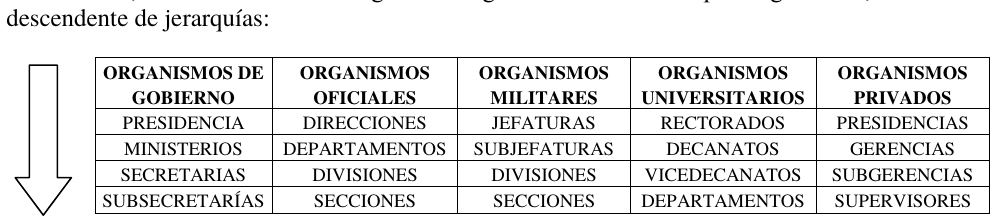
\includegraphics[width=1.00\linewidth]{figuras/fig_p021_12.png}
\end{center}

Las responsabilidades, funciones, atribuciones y autoridades son detalladas en el libro orgánico de la organización que puede adoptar diferentes nombres o designaciones dependiendo de la organización en particular.


% ---- página 22 ----

\subsubsection*{EJEMPLOS DE ESTRUCTURAS ORGÁNICAS}
La estructura lineal o llamada también militar es la más adecuada para organizaciones pequeñas, quedan bien definidas las autoridades y tienen la capacidad de transmisiones rápidas de órdenes, pero la organización tiene una fuerte dependencia funcional de los órganos intermedios. La organización lineal y conjunta es una variante de la anterior a la que se le ha agregado un órgano asesor que tiene la facultad de aconsejar a la autoridad en la toma de decisiones pero no tiene responsabilidad. La organización combinada es la más utilizada por las organizaciones actuales, no tiene una dependencia funcional tan limitante como la lineal o militar, pero requiere una mejor organización de las tareas y una buena comunicación entre los órganos.


\begin{center}
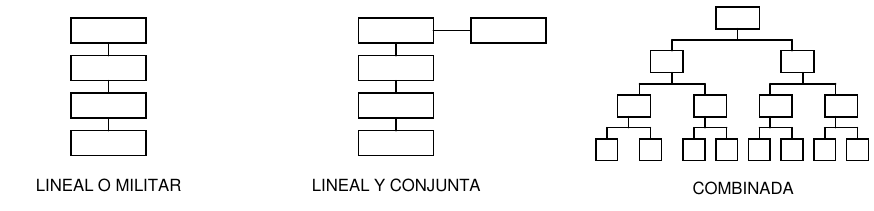
\includegraphics[width=0.89\linewidth]{figuras/fig_p022_13.png}
\end{center}

Las estructuras tipo grupo comercial o autónomo son adecuadas para las organizaciones comerciales pequeñas, presentan las mejores características de respuesta con el objetivo de satisfacer al cliente, las estructuras en forma de equipos de trabajo son adecuadas para pequeñas organizaciones con culturas de trabajo en equipo, los órganos que funcionan altamente integrados, la atmósfera de trabajo es estable, debe gobernar la franqueza, la cooperación y la confianza, un solo directivo es elegido como coordinador para dirigir al equipo.


\begin{center}
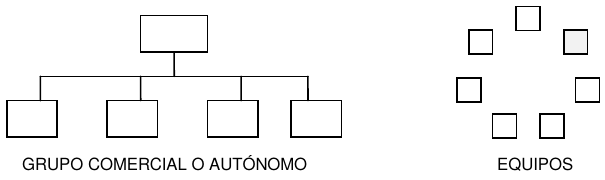
\includegraphics[width=0.62\linewidth]{figuras/fig_p022_14.png}
\end{center}

\subsubsection*{ORGANIGRAMA DE ORGANIZACIONES AERONÁUTICAS}
En la actividad aeronáutica, las organizaciones deben cumplir con regulaciones que establecen ciertos condicionamientos en la constitución de su organigrama para ser aprobado, como también el personal propuesto para ocupar los cargos directivos (RAAC 121 para transporte aerocomercial regular, RAAC 135 para empresas de transporte aerocomerciales no regulares y RAAC 145 para organizaciones de mantenimiento aeronáutico), la estructura orgánica, las funciones, atribuciones y responsabilidades quedan definidas en el Manual General de la Empresa que es aceptado por la Autoridad Aeronáutica.

Este condicionamiento se refiere solamente a los órganos que realizan tareas técnicas, de modo que los órganos que tienen a cargo la supervisión de las tareas realizadas sobre el material aeronáutico sean independientes y se encuentren por sobre los órganos controlados para asegurar una correcta supervisión. Por ejemplo: El siguiente organigrama parcial que podría corresponder al área técnica de una empresa aérea:


% ---- página 23 ----

\begin{center}
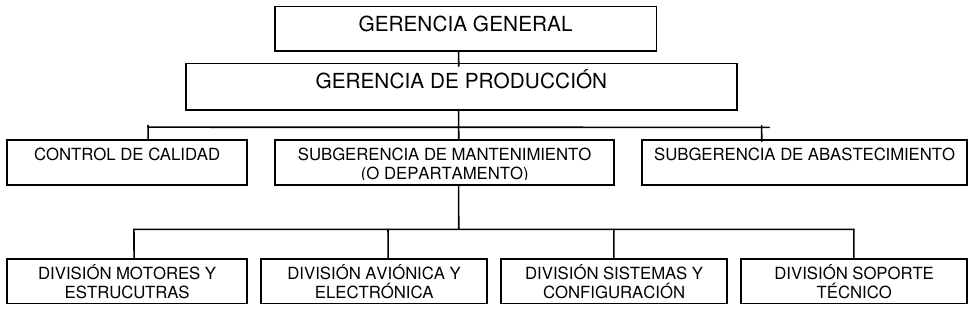
\includegraphics[width=0.99\linewidth]{figuras/fig_p023_15.png}
\end{center}

Las organizaciones diseñan su estructura formal de manera de ser eficientes y funcionales, continuamente modifican su estructura adaptándola a los requerimientos de su actividad, los cambios en las estrategias y objetivos, redefiniendo las responsabilidades, funciones, reasignando tareas, creando nuevas divisiones, tercerizando otras y esta actividad continua a lo largo de la vida de las organizaciones.

\section*{ADMINISTRACIÓN}
\subsubsection*{INTRODUCCIÓN}
Las organizaciones necesitan ser administradas y estas tareas son encargadas a una persona en las pequeñas organizaciones, o grupo de personas en las grandes organizaciones cuando el volumen y la complejidad de las funciones que realizan alcanzan cierto desarrollo.

\subsubsection*{CONCEPTO}
\textbf{La administración es la conducción racional de las actividades de una organización, con o} \textbf{sin ánimo de lucro.}

En una organización plenamente racionalizada y funcionando perfectamente todas las contingencias normales estarían prevista y las decisiones se tomarían automáticamente, esta sería la situación ideal de una organización. Una organización se considera tanto mejor organizada cuanto más se le aproxime.

El termino administración se puede tomar en dos sentidos, como actividad y como ciencia. Considerando a la administración como actividad, es el conjunto de tareas asignadas a una persona (o grupo de personas) con la finalidad de determinar los objetivos generales, organizar, mandar, dirigir, coordinar, controlar, crear el plan de dirección y organizar la estructura de la organización.

En cambio si lo consideramos como ciencia constituye un conjunto de saberes, conocimientos y reglas necesarias para gestionar actividades de negocios, servicios, etc.

La administración es imprescindible para la existencia, la supervivencia y el éxito de las organizaciones. Sin ella, las organizaciones jamás encontrarían condiciones para existir y crecer. La administración de las instituciones tiende a mejorar la calidad de las organizaciones y el funcionamiento de las mismas.

\textit{La Teoría General de la Administración (TGA) }es el campo del conocimiento humano que se ocupa del estudio de la administración en general, independientemente de si ésta se aplica en organizaciones con fin de lucro (empresas) o en aquellas que no lo tienen.


% ---- página 24 ----

ACLARACIÓN: En la bibliografía anglosajona los conceptos de organización y administración son opuestos a los utilizados en nuestro país, por ejemplo la National Aeronautics and Space Administration (NASA), es la organización que se ocupa de las actividades espaciales en los EEUU, aquí el termino administración es utilizado como sinónimo de organización.

\subsubsection*{FUNCIONES DE LA ADMINISTRACIÓN}
Planeamiento: Es la acción y efecto de prever los factores que incidirán en las actividades, por medio de una guía de procedimientos llamada plan.

Un plan se considera óptimo cuando reúne las siguientes cualidades:

\begin{itemize}
  \item Unidad: Deber responder a un solo objetivo.
  \item Continuidad: El logro del fin propuesto debe lograrse en un lapso definido.
  \item Flexibilidad: El plan debe poder adaptarse a cambios previsibles sin variar el objetivo.
  \item Precisión: Sus resultados deben obtenerse con la máxima precisión compatible con el futuro previsto.
  \item Practicabilidad: Debe ser materialmente posible su realización, en tiempos y costos compatibles.
\end{itemize}
Organización: Se establece definiendo claramente la autoridad, las atribuciones, responsabilidades y funciones de cada órgano, mediante la confección de la estructura orgánica y del manual orgánico, a fin de poner en ejecución el plan convenido con el máximo de economía. Mando: El mando se ejerce mediante pronunciamiento de órdenes que pueden ser verbales o escritas en forma de directivas, instrucciones, o de cualquier otro tipo que la organización considere adecuado.

El mando se ejercita eficientemente cuando se aseguran las siguientes condiciones:

1. Ordenes claras: Quien ordena debe asegurarse que las ordenes fueron bien interpretadas y que son posibles de realizarse con los medios disponibles.

2. Disciplina: Se mantiene respetando la línea de mando, dando el ejemplo, controlando el cumplimiento de las directivas y sancionando las faltas de cumplimiento.

3. Reconocimiento: Se basa en el reconocimiento del personal más capaz, la recepción de iniciativas, aseguramiento de la continuidad de las actividades, recordar los objetivos de la empresa y la contribución que cada uno aporta al mismo.

4. Autoridad: Para ejercerlo se debe tener las siguientes cualidades: Competencia, energía, inteligencia, responsabilidad y dinamismo.

5. Eficacia: Debe ser accesible al personal, no ocasionar pérdidas de tiempo.

Coordinación: Es el proceso o acción de crear y mantener relaciones adecuadas entre las funciones, los factores físicos y el personal, se debe promover y asegurar la unidad del esfuerzo para cumplir con el objetivo impuesto.

Control y Vigilancia: Esta función tiende a comprobar los resultados reales obtenidos en las actividades con lo previsto a fin de tomar las decisiones necesarias para rectificar lo que se aparte del plan. El control se pone en práctica vigilando los siguientes elementos: Del personal se controla su eficiencia y tiempos; del equipo se controla sus cualidades, cantidades, su empleo y mantenimiento; de las actividades se controla para eliminar las tareas inútiles y modificar los procedimientos para asegurar la productividad y la economía, mediante la comprobación con los presupuestos determinados.


% ---- página 25 ----

\subsubsection*{CUESTIONARIO 2}
1. ¿Qué es la división del Trabajo?

2. ¿Qué limitaciones tiene la división del trabajo?

3. Organigrama: ¿Qué es?, ¿qué nos muestra?, ¿quién lo confecciona?, ¿puede variar en el tiempo?

4. ¿Los principios orgánicos dan recomendaciones o reglas?

5. ¿Qué establece el principio de la delegación de autoridad?

6. ¿Cuáles son las ventajas de una estructura orgánica lineal o militar?

7. Ordenar los siguientes órganos de acuerdo a su jerarquía, asignándoles números de 1 a 4.


\begin{center}
\small
\begin{tabular}{|p{\dimexpr0.030\linewidth-2\tabcolsep\relax}|p{\dimexpr0.211\linewidth-2\tabcolsep\relax}|p{\dimexpr0.030\linewidth-2\tabcolsep\relax}|p{\dimexpr0.226\linewidth-2\tabcolsep\relax}|p{\dimexpr0.030\linewidth-2\tabcolsep\relax}|p{\dimexpr0.211\linewidth-2\tabcolsep\relax}|p{\dimexpr0.030\linewidth-2\tabcolsep\relax}|p{\dimexpr0.211\linewidth-2\tabcolsep\relax}|}
\hline
 & DIRECCIÓN &  & SECCIÓN &  & DIVISIÓN &  & DEPARTAMENTO \\ \hline
\end{tabular}
\end{center}

8. ¿Cuáles son las cualidades que debería tener un plan?, ¿quién establece el plan?, ¿quién establece el objetivo de la organización?

9. ¿Cuándo el mando se ejercita eficientemente?

10. ¿Por qué las organizaciones se consideran como sistemas?

11. ¿Cuáles son las funciones de la administración?


\begin{center}
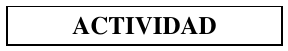
\includegraphics[width=0.29\linewidth]{figuras/fig_p025_16.png}
\end{center}

Una empresa de transporte aéreo informa sobre la estructura orgánica a rediseñar en la compañía a fin de mejorar la eficiencia de su accionar, con miras a contrarrestar la fuerte competencia del mercado, las funciones que se desempeñan en la empresa son:

Planificación Radiocomunicaciones Mantenimiento de aviones  Marketing Control de calidad

{\centering Traducciones\par}

Administración de material  Impuestos Inspección y control

{\centering Seguridad edilicia\par}

Plantas de poder Mantenimiento edilicio Montaje

{\centering Almacenes\par}

Electricidad del avión

{\centering Depósitos\par}

Mecánica

{\centering Asuntos legales\par}

Control de costos

{\centering Obtención de capital\par}

Liquidación de Sueldos y Jornales  Cuentas Biblioteca técnica Instrumental del avión Capacitación del personal  Inversiones Balance contable

{\centering ventas\par}

Para elaborar el organigrama con las funciones enumeradas, se siguen los siguientes pasos:

1. Clasificar las funciones según su clase (“A” si son administrativas, “C” contables, “T”

técnicas, “F” financieras, “P” personal).

2. Dentro de cada clase, se establece la jerarquía de los órganos componentes de las funciones a realizar (dirección, departamento, división, sección) 3. En borrador se elabora tentativamente un primer organigrama.

4. Se combinan todos los organigramas realizados en el curso.


% ---- página 26 ----

\section*{REINGENIERÍA}
\subsubsection*{INTRODUCCIÓN}
Para sobrevivir, para ser rentables, hay empresas que necesitan revertir su declinación y fracaso mediante un esfuerzo que las haga recuperar y volver a ser exitosas. Hay empresas que deben adaptarse a cambios del entorno, que ahora se dan cuenta, serán permanentes. Hay otras, que en nuestros días, deben preparase para un contexto diferente de mayor competencia, apertura de la economía, desregulación de mercados, cambios de costumbres, etc. El proceso viene realizándose silenciosamente desde los años 70 / 80, compañías que se cierran, fusionan, cambian de orientación o tamaño, cada empresa lo realiza de la mejor manera posible y es usual que se cometan errores (este tipo de transformaciones no se realiza todos los días). En nuestro país, el contexto complicado económico ha obligado a más de una empresa y organismos del gobierno a hacer una reestructuración. En los países desarrollados se han producido fenómenos parecidos, a veces, por otras razones, competencia internacional, evolución del precio de la energía, avance tecnológico, la mayor competencia mundial y los cambios tecnológicos han sido algunas de las razones por las cuales empresas, grandes y chicas, se están reestructurando. Restaurar no es eliminar personal y tomar medidas de austeridad, es mucho más: Una revisión crítica de la situación y la toma de medidas.

Bajo diferentes palabras: \textbf{Restructuring, Downsizing, Turnaround, Reingeniería}, el proceso va siempre acompañado por una revisión crítica de la estrategia empresarial, realizándose los cambios estructurales y estratégicos para volver a ser una empresa sana y rentable, evitándose el deterioro en el tiempo que obligue a efectuar lo mismo años más tarde.

\subsubsection*{LAS SEÑALES EXTERNAS E INTERNAS}
El indicador último que señala la necesidad de una reestructuración es, quizás, los resultados de la empresa en relación a la competencia (su competitividad). Sin embargo, el tema no es simple. La evaluación de las ventas, participación en el mercado, rentabilidad, punto de equilibrio, y costo financiero pueden ser indicadores que llamen a la reflexión. Pero también hay señales internas: Tomas de decisiones lentas, excesivo control, demasiadas reuniones, burocracia (procedimientos engorrosos y con demasiados pasos).

\subsubsection*{RELACIÓN ESTRUCTURA – ESTRATEGIA}
Los investigadores notaron hace tiempo que la estrategia tiene influencia en la estructura de las organizaciones, el concepto de estructura tratado en este capítulo es más abarcativo que los estudiados anteriormente, en la bibliografía de administración de empresas la palabra estructura está muy asociada con la de estructura organizacional. Más de una persona se imagina la representación gráfica de un organigrama cuando la escucha. Aquí se intentará usar un concepto más amplio, se concebirá a la estructura de la empresa como aquellos aspectos físicos, administrativos, humanos, financieros y legales cuyo cambio demanda cierto tiempo. En el cuadro puede verse un enfoque más amplio de los aspectos que integran el concepto de estructura de una empresa:


% ---- página 27 ----

\begin{center}
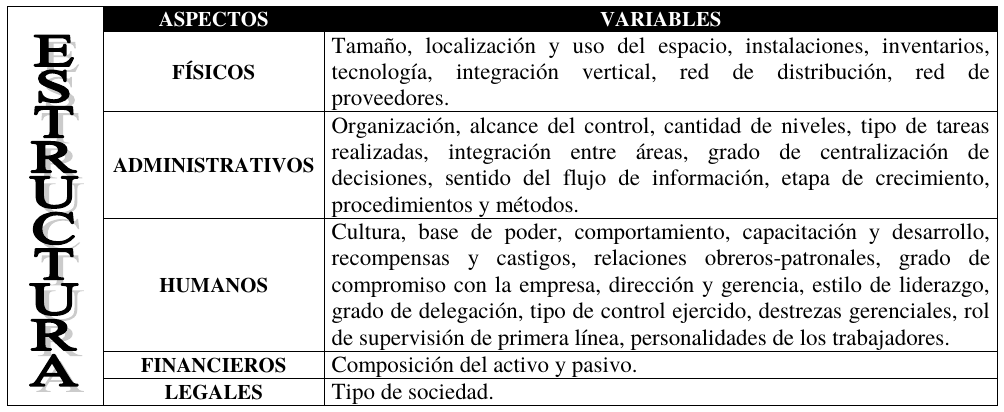
\includegraphics[width=1.00\linewidth]{figuras/fig_p027_17.png}
\end{center}

\subsubsection*{¿ES NECESARIO REESTRUCTURAR?}
Aceptado el concepto amplio de estructura, la pregunta inmediata es: ¿Por qué hay que reestructurar? (es decir cambiar la estructura). Cuando se habla de procesos de reestructuración no se piensa en modificaciones menores de estructura por adaptación al entorno, sino en los esfuerzos importantes de las empresas para cambiar significativamente la estructura existente La respuesta involucra varios aspectos:

a) Determinados por cambios importantes en el entorno, por ejemplo: Aparece una novedad tecnológica importante en el mercado, el consumidor cambia de gusto, caen las protecciones aduaneras, se modifican los precios internacionales.

b) Determinados por razones internas, por ejemplo: La empresa debe recuperar rentabilidad, la empresa quiere mayor flexibilidad para encarar una estrategia diferente, la empresa cambia de propietario.

\subsubsection*{¿CUÁNTO ES EL TIEMPO DISPONIBLE?}
El tiempo disponible para reestructurar es muy limitado y obliga a tomar medidas drásticas y de rápido efecto. El tiempo disponible determina el enfoque de la reestructuración, la posibilidad de hacer estudios detallados posteriores, el tipo de medidas a adoptar y la naturaleza del proceso de cambio. En general el tiempo dependerá de la gravedad de la crisis, pero se disponen de meses para las primeras etapas.

\subsubsection*{LA FINANCIACIÓN DE LA REESTRUCTURACIÓN}
Se necesitan recursos para encarar una reestructuración, encarar una nueva acción comercial, modernizar una línea de producción, computarizar un sistema de cobranzas, tecnificar la producción, hacer estudios y análisis de las estrategias, etc. requieren dinero. Muchas veces la empresa ha llegado a una situación tan difícil que en que ni siquiera tiene capital suficiente, lo que origina un círculo vicioso. Se deben estudiar todas las posibilidades como adquirir nuevos socios, financiación externa de bancos, ventas de activos.

\subsubsection*{EL SENTIDO DE UNA REESTRUCTURACIÓN}
Una reestructuración no se hace todos los días y no se puede hacer frecuentemente en el sentido que aquí se presenta. Básicamente consiste en un cambio significativo de algunas o de todas las variables estructurales que se realiza en un período limitado (meses) para sanear la empresa. Si la reestructuración es adecuada, la empresa tendrá las bases para ser eficiente y rentable.


% ---- página 28 ----

Por ejemplo las variables a reestructurar pueden ser:

a) Aspecto físico: Se pueden reducir las cantidades de oficinas, crear oficinas de ventas en otros países, vender o alquilar espacio no utilizado, vender o alquilar activos no utilizados, no utilizar tecnología obsoleta o ultramoderna, disminuir los recorridos de las redes de distribución, mejorar las relaciones con los proveedores.

b) Aspectos administrativos: Restablecer el orden y la disciplina, reducir la cantidad de niveles, automatizar algunas funciones, fomentar la interacción entre áreas, incentivar premiando el buen desempeño, mejorar los métodos y procedimientos, el control. c) Aspectos humanos: Mejorar la cultura de una organización, transformar el ambiente de apatía, faltas de interés, resignación, temor por el futuro, en un clima de optimismo realista, perseverancia, confianza, y espíritu de equipo.

d) Aspecto financiero: Cambios de plazos en créditos, ventas y alquileres de activos no utilizados, aumento del capital de trabajo.

e) Aspectos legales: Transformar las S.R.L. en S.A., dividir la empresa en varias empresas legalmente diferentes.

\subsubsection*{EL PERSONAL Y LA CULTURA}
En los últimos años se han observado ciertas tendencias en las características de la estructura humana y la cultura del personal, solo como ejemplo se listan a continuación algunas de las características buscadas en estos cambios:

- Base de poder: Centrado en el conocimiento y no por la posición.

- Comportamiento adaptativo.

- El énfasis en la capacitación y el desarrollo de personal.

- Recompensas grupales basadas en la innovación y los resultados generales de la empresa.

- Madurez en las relaciones obrero-patronales.

- Mayor participación y poder al personal.

- Obsesión por el mejoramiento continuo de la empresa y el mantenimiento del liderazgo.

- Compromiso con la empresa.

- Creatividad.

- Gerentes con estilos de liderazgo más participativo.

- Reemplazo del control por el autocontrol.

\subsubsection*{ALGUNOS EJEMPLOS DE REESTRUCTURACIÓN DE EMPRESAS}

\begin{recuadro}
\subsubsection*{HUGHES AIRCRAFT}
Parte de la GM Hughes Electronics, deseaba mejorar la fabricación de satélites, el vicepresidente de operaciones creo grupos multidisciplinarios para revisar todo el proceso. Se llego a que había 131 temas en donde se podían hacer mejoras importantes y que 30 de ellos eran los más urgentes. Haciendo una serie de cambios aparentemente pequeños (como mover una agujero de ¼ de pulgada para que un inspector pudiese insertar más fácilmente un equipo de testeo), Hughes disminuyo el tiempo para construir el control de proceso de un satélite (la mente del satélite) de 45 a 22 semanas, ahorrando millones de dólares.
\end{recuadro}

% ---- página 29 ----

\begin{recuadro}
\subsubsection*{INNOVACIONES Y CAMBIOS ESTRATÉGICOS}
LUCIANO BENNETTON era el mejor ejemplo de innovación y éxito empresarial en Italia. Comenzó casi desde la nada y construyó el emporio de la moda de 5000 negocios con 1200 millones de dólares en ventas en 80 países. Un intento de diversificación en servicios financieros termino mal en febrero de 1990 lo que redujo sus márgenes. Los nuevos mercados en Polonia, Hungría y Checoslovaquia han comenzado bien.

ANGELO COSTA fue uno de los primeros en comprar buques Liberty americanos, excedentes de la Segunda Guerra Mundial y transformarlos en los cruceros Costa. La empresa tuvo ganancias por 15 millones de dólares en 1989 se ofrece cruceros lujosos con servicios personalizados desde Europa al Caribe, se diseñaron estrategias comerciales para los próximos 10 años por la incertidumbre de la desregulación de las tarifas aéreas europeas que se prevén podrían afectar el futuro de los viajes.
\end{recuadro}

\begin{recuadro}
\subsubsection*{KODAK}
Ha estado luchando por varios años para reducir sus costos, con resultados cuestionables. Desinversiones, cierres de plantas, consolidaciones, despidos masivos. Luego de varias reestructuraciones, la empresa tuvo en 1989, una pequeña utilidad operativa, entre 1989 y 1990 unas 5000 personas abandonaron la empresa.

En ese proceso de mejora, no del todo exitoso, una revolución se ha generado en la división que manufactura componentes de precisión. Los operarios de la línea de ensamble que hacen los cassettes de rayos X y componentes para el film Kodak, deciden ahora su horario, controlan su productividad y arreglan sus máquinas. Hace tres años uno de los operarios tenía la tarea de operar una máquina por ocho horas diarias, ahora coordina con sus compañeros el control estadístico del proceso, se reúne con proveedores, entrevista a los candidatos interesados a ingresar a la empresa y ayuda en la implementación del Just-in-time. El mejor uso de la mano de obra ha permitido que este sector haga en un turno lo que antes requería tres. Movilizaron el recurso más fantástico que tiene la empresa: La gente.
\end{recuadro}

\begin{recuadro}
\subsubsection*{COLGATE – PALMOLIVE}
Intentó reducciones masivas de personal en los años 80 cuando deseaba bajar costos en la división tecnológica. El vicepresidente ejecutivo y máximo responsable del área tecnológica explico que esas reducciones no fueron permanentes, la empresa agrego posteriormente lo que se necesitaba. Se hizo un relevamiento de cómo los gerentes y empleados distribuían su tiempo. Los resultados fueron sorprendentes: En lugar de preocuparse sobre como podrían convertir a los dientes en más blancos o la ropa en más limpia, dedicaban mucha energía en supervisar e informar. También estaban preocupados por el diseño de nuevas fábricas, tarea que tenía poco que ver con la responsabilidad principal de inventar y mejorar productos. Después del relevamiento, se eliminaron dos niveles de supervisión y se contrato externamente el diseño de fábricas. Para liberar a los científicos de las tareas de compras o presupuestos se incrementó el personal de apoyo. Se cerraron dos de los cuatro laboratorios importantes en el mundo y se redujo en 40\% el número de proyectos de investigación. Para mejorar la eficiencia del personal se cambio el agrupamiento funcional. Se eliminaron las viejas divisiones de investigación básica, procesos y empaques, y se agrupo al personal en grupos por conjunto de productos. El grupo así conformado ha generado un flujo continuo de nuevos productos y Colgate calcula que ha ahorrado 40 millones de dólares en los últimos tres años.
\end{recuadro}

% ---- página 30 ----

\subsubsection*{CUESTIONARIO 3}
1. ¿Cuál es el concepto de Estructura que se ha utilizado?

2. ¿Cuál es la magnitud de los cambios que involucra un proceso de reestructuración?

3. ¿Qué motiva a una empresa a reestructurarse?

4. Teniendo en cuenta el objetivo que se desea obtener, ¿pueden considerarse sinónimos los términos “reestructuración” y “aumento de eficiencia”?

5. ¿A qué se llama integración vertical?

6. ¿Qué tendencias en el aspecto humano de una empresa buscan las empresas modernas?

7. ¿Quién realiza la reestructuración en una empresa?

8. ¿Qué medidas se toman para reducir personal?

9. ¿Qué indicadores determinan la necesidad de la reestructuración de una empresa?

10. ¿Cómo se determina la situación actual de una empresa?

11. ¿Cuáles son las consecuencias inmediatas de una reestructuración?


% ---- página 31 ----

\subsubsection*{CONTENIDOS DEL NÚCLEO TEMÁTICO TERCERO}
Relaciones Humanas. La Estructura Formal y La Estructura Humana. Características del ambiente Laboral. Comunicación. Cultura organizacional. Cambio y Resistencia al Cambio.

\section*{RELACIONES HUMANAS}
\subsubsection*{INTRODUCCIÓN}
Las relaciones humanas es una técnica social en el sentido preciso de ciencia social aplicada. Como ciencia habrá que juzgarla por la solidez de los datos científicos en que se apoya, como aplicación por los fines a los que se orienta. La ciencia en la que se apoya son las la psicología y la sociología. Debieron pasar muchos años para que ambas confluyesen en el estudio de la conducta del hombre en el medio laboral.

Uno de los problemas fundamentales de la psicología de las relaciones humanas es el que se refiere a los procedimientos necesarios para mantener la paz con nuestros semejantes y evitar toda clase de conflictos que puedan surgir en el trato diario. Por eso es preciso que aquellas personas que ocupan puestos de autoridad, cuyas acciones y decisiones puedan afectar (para bien o para mal) a la organización, comprendan el significado y la naturaleza intima de estas. Que sepan ver las facetas humanas, que no se limiten a los procesos técnicos y económicos, que se den cuenta de la importancia de su papel, la trascendencia de sus decisiones y que prevean las consecuencias de sus acciones.

En las organizaciones no solo hay que tomar decisiones sobre problemas técnicos y económicos, sino también humanos, y más precisamente no hay problemas únicamente técnicos o económicos o humanos todas las decisiones involucran estos tres aspectos, y más todavía cualquier decisión tendrá consecuencias técnicas, económicas y humanas.

\subsubsection*{DEFINICIÓN}
Una definición relativamente rigurosa del objetivo de la teoría de las relaciones humanas dice que procura conseguir una organización que no solo sea eficiente desde el punto de vista técnico y económico sino al mismo tiempo satisfactoria para los individuos y los grupos que la forman. Dicho de otra forma, es una teoría científica de la organización del trabajo en sus aspectos humanos, pero este aporte de las relaciones humanas no se limita a mejorar solo el estado de los trabajadores o de la organización, es además una ayuda para conseguir el tipo de sociedad que todos deseamos, forjando organizaciones satisfactorias, no solo en términos de producción, sino también en cuanto a las aspiraciones y modos de vida de los trabajadores.

\subsubsection*{LA ORGANIZACIÓN}
LA ESTRUCTURA FORMAL Y LA ESTRUCTURA HUMANA Las organizaciones están formadas por un grupo de personas que colaboran de algún modo para alcanzar el objetivo establecido por la organización. Esto implica la existencia de una autoridad y la división de funciones, de aquí se deriva la estructura orgánica estudiada anteriormente, que coordina la actividad de los diferentes miembros. Esta estructura que llamamos formal se traduce en las jerarquías y la división del trabajo representadas gráficamente con el organigrama, los reglamentos y las normas de actuaciones, circulación de materiales, mano de obra, ordenes de trabajo, métodos de inspección, es la que se escribe en papel y se define por formulas. Pero toda organización tiene una segunda estructura que, para diferenciarla de la anterior, la llamaremos informal.

Las organizaciones están formadas por hombres y esto tiene al menos dos consecuencias importantes:


% ---- página 32 ----

En primer lugar suponiendo que se pudiera medir, en cada uno de los integrantes de la organización, sus conocimientos, sus aptitudes, y sus capacidades, ello no nos informaría sobre la medida en que se pondrían en juego estas capacidades, sobre su interés y entusiasmo en el trabajo. Claro que podemos suponer que con una cantidad adecuada de estimulo económico, compensada con cierta dosis de amenazas (política de la zanahoria y el palo) el trabajador - o el directivo para el caso es lo mismo- rindan todo su esfuerzo. Pero esto es un modealización simplista y burda del comportamiento del hombre en el ámbito laboral, que la realidad se encarga de desmentir. Cada hombre tiene sus propios motivos, conscientes o inconscientes, para actuar como lo hace, y estos motivos solo en parte son económicos.

En segundo lugar el hombre no trabaja solo sino junto con otros, formando grupos con ellos. El organigrama y los reglamentos indican el contenido y las formas de estas relaciones: “A” pasar el material a “B”, “C” inspecciona lo que “B” ha mecanizado, “D” informa a la dirección sobre lo producido y etc. Pero la realidad es mucho más complicada. “A” conversa con “B”, lo respeta y lo ayuda en su trabajo, mientras que le disgusta el aire de superioridad de “C” y hace todo lo posible por obstaculizar su función. ”D” informa a la dirección, pero redacta su informe con la vista fija en la opinión del jefe de departamento y como lo comparará con el que reciba de “E”.

Los lugares de trabajo no son solamente grupos de personas unidas por relaciones funcionales y jerárquicas, es un grupo humano con simpatías y antipatías, rencores y amistades, usos y costumbres, con actitudes y normas de conducta aceptadas por todos los miembros.

De esta forma aparece la nueva cara de la organización, la estructura informal o espontánea calificada como estructura humana. Esta cara de la organización integradas por grupos de personas con distintos modos de vida, cultura, intereses, necesidades y aspiraciones diversas, subordinados a otras personas, enemigos o amigos, de contacto diario, este reino de sentimientos y emociones, encontronazos y rumores, camarillas, bromas y chistes de vestuario representa la faceta humana de todas las organizaciones.

Si queremos definirla con cierta precisión diremos que: La estructura informal es la resultante de las relaciones humanas individuales y colectivas entre los integrantes de la organización, a la situación en que los coloca la estructura formal.

\subsubsection*{EL AMBIENTE LABORAL}
\begin{itemize}
  \item LA ORGANIZACIÓN PERFECTA
\end{itemize}
La organización perfecta no existe, pero ¿qué condiciones debería reunir en el aspecto humano para que sea satisfactoria para los trabajadores?

Debería ser aquella que tenga algún significado personal para cada uno de los miembros de la organización. Esto equivale a que la tarea asignada a cada uno, ocupe la mayor parte posible de sus capacidades, incluida su iniciativa, creatividad y su sentido de responsabilidad de modo que no solo conozca los resultados de su labor, sino también se espere su colaboración en el objetivo común.

Que su trabajo sea reconocido dentro y fuera de la organización y que este trabajo constituya un aporte valioso para el objetivo de la organización.

Por otra parte, a través de su trabajo, cada individuo ansía poder concretar sus fines personales, fines económicos en relación con su nivel de vida como también en los demás ordenes en los que el trabajo se pueda satisfacer como la seguridad, confianza, prestigio, progreso, comodidad, conocimiento, desafío, etc.


% ---- página 33 ----

No menos importante lo constituye el entorno del trabajador: Un ambiente de trabajo enmarcado en valores, cooperación, confianza, colaboración y respeto.


\begin{center}

\includegraphics[width=0.99\linewidth]{figuras/fig_p033_18.png}
\end{center}

En los últimos años, los estudios sobre relaciones humanas, se han orientado hacia este fin práctico. Su objetivo inmediato se ha convertido en mejorar la eficiencia y productividad de las organizaciones en un concepto amplio que incluya el aspecto humano y fomentando entre los trabajadores una actitud positiva hacia la situación laboral.

\begin{itemize}
  \item LA COOPERACIÓN
\end{itemize}
Las relaciones que se dan entre automovilistas que manejan en una autopista son cooperativas. Los conductores se mantienen en sus carriles y cuando superan a otro automovilista lo hacen por la izquierda. Cooperar significa co-operar, es decir operar con otros. Las leyes de tránsito permiten que los automovilistas puedan cooperar, o también operar con otros automovilistas, con el propósito de circular en forma segura, las leyes establecen explícitamente las reglas de cooperación entre automovilistas. Pero ¿cómo se relaciona este concepto en el ámbito laboral? Durante la jornada laboral cooperamos con las personas que nos relacionamos y nos relacionamos con las personas con las que cooperamos. Cuando un jefe asigna un trabajo para realizar a un empleado, está solicitando una operación al empleado, es decir que el empleado ejecute ciertas acciones, (acomodar mercadería en un depósito, llenar los depósitos del sistema hidráulico de una aeronave, planificar las tareas de mantenimiento de una empresa aérea, etc.), el empleado coopera con el jefe en la tarea designada. A su vez para realizar las acciones requeridas por el jefe, el empleado debe cooperar con otros empleados (para el ejemplo del llenado de los depósitos del sistema hidráulico requerirá la cooperación de quien provee los envases de liquido hidráulico, de quienes proveen los andamios, de otros empleados que estén trabajando en la aeronave, de quienes asientan en los registros la carga de liquido hidráulico, etc.), los empleados operan en conjunto para realizar la acción solicitado por el jefe. Todos los trabajos establecen de por sí la cooperación, debido a que no existen trabajos que no estén vinculados a la cooperación de otras personas. Un piloto de una aeronave comercial en vuelo coopera con otros pilotos de aeronaves, el controlador de tráfico aéreo, el personal de cabina y el copiloto, para realizar su trabajo.

En este momento es necesario hacer una distinción: No son sinónimos la cooperación y la colaboración. La colaboración es la ayuda brindada en la ejecución de una tarea, y la cooperación es la ejecución de una tarea entrelazada con la tarea de otras personas. En la autopista cooperamos con otros conductores pero no necesariamente colaboramos.


% ---- página 34 ----

Los trabajos que requieren una gran participación de los trabajos de otras personas, exigen un gran esfuerzo de coordinación y comunicación, este esfuerzo se incrementa si además los intervinientes hablan diferentes idiomas o profesiones diferentes o se encuentran distanciados. Por último se puede comentar que las organizaciones, para brindar un producto, deben cooperan con otras organizaciones o personas externas a la organización, por ejemplo una empresa aérea coopera con la organización que le provee el catering, se coordinan los horarios, el tipo de servicio, el tipo de alimento, las cantidades, los lugares de entrega, etc. con el fin de operar en conjunto.

\begin{itemize}
  \item LA DIVISIÓN DEL TRABAJO
\end{itemize}
La excesiva división del trabajo, como el hacer por un lado y el pensar y decidir por el otro lado, la monotonía y el aburrimiento de trabajos demasiado especializados, ha llegado a ser un símbolo del trabajo racionalizado en la actualidad, no está directamente relacionados con la repetición en sí misma, sino con la falta de significado del trabajo para el individuo. Esta insatisfacción en el trabajo influye sobre la moral laboral y sobre el rendimiento. Para contrarrestar estos efectos se ha desarrollado una reacción conocida como “ampliación de las tareas”, que pretende enfrentar al trabajador con tareas más complejas y más responsables, otorgándosele cierto poder de decisión, con la esperanza de que las tareas resulten satisfactorias y significativas.

\begin{itemize}
  \item EL GRUPO DE TRABAJO
\end{itemize}
Cada trabajador tiene amistades y aversiones particulares, personas a las que se siente próximo, cuyos sentimientos y valores respeta y otros a quienes es indiferente, de estas relaciones nacen los grupos, los jefes espontáneos y sus seguidores, los grupos que se oponen entre si y aquellos que permanecen acordes en opiniones que varían, desde si debe abrirse o cerrase una ventana hasta si debe o no hacerse huelga.

El grupo de trabajo se define como el conjunto de personas interdependientes y constituye verdaderamente un cuerpo y no un conglomerado o colección de individuos. En el seno de ese grupo se desarrolla un sistema de tensiones positivas o negativas, correspondientes al juego de los deseos y de las defensas, la conducta del grupo consiste en un conjunto de operaciones tendientes a resolver esas tensiones y a restablecer un equilibrio más o menos estable. Estas tensiones tendientes a unir o romper los enlaces pueden ser muy variadas (socio-afectivos, cohesión, jerárquicas, operativos-funcionales, conformismo). La cohesión en el seno del grupo siempre se refuerza frente a amenazas externas. El comportamiento laboral de cada individuo está condicionado por su pertenencia al grupo, basta con modificar el grupo en el que está incluido para modificar sensiblemente su comportamiento.

\begin{itemize}
  \item EL EQUIPO DE TRABAJO
\end{itemize}
El grupo tiene un jefe jerárquico designado por la organización, cuya misión es hacer aceptar al grupo los objetivos de la organización. Organizado un grupo de trabajo y designado un jefe, se deben respetar ciertas pautas de comportamiento interpersonal para que el grupo trabaje como equipo altamente integrado y alcance los objetivos de su formación, todos los miembros del equipo deben ajustarse a este código de conducta. Las siguientes pautas son algunos ejemplos, téngase en cuenta que representan la generalidad debido a los diferentes grupos que podemos encontrar en el ámbito laboral:

\begin{itemize}
  \item Asegúrese de haber comprendido el enunciado del problema a resolver y que todos los integrantes también lo han comprendido.
  \item Critique ideas y no a las personas.
\end{itemize}

% ---- página 35 ----

\begin{itemize}
  \item Respete los tiempos de cada uno.
  \item La única pregunta tonta es la que no se hace.
  \item Enfocarse en el objetivo de creación del grupo.
  \item Todos los miembros del equipo son responsables del progreso del trabajo.
  \item Evite el liderazgo directivo.
  \item Vea las diferencias de opiniones como un aporte, más que como un obstáculo.
  \item Controle sus sentimientos.
  \item El silencio es a menudo tomado como aceptación.
  \item Las reuniones deben conducirse ordenadamente.
  \item El jefe debe evitar emitir opinión hasta que todos hayan sido escuchados.
  \item No cambie su forma de pensar solo para lograr un acuerdo y evitar conflictos.
  \item Utilice la realimentación como confirmación de haber entendido la idea del otro.
  \item CONFLICTOS
\end{itemize}
En la vida laboral (como también en la vida en sociedad) hay relaciones cooperativas pero también conflictivas. Los conflictos consisten en los enfrentamientos abiertos entre personas o grupos de personas que desean prevalecer sobre otros individuos o grupos de individuos en pos de un objetivo excluyente. En nuestro contexto nos referimos a los conflictos que surgen entre jefes y subordinados, empresas y obreros, entre empleados de secciones, la gerencia de calidad de una organización con los auditados, sección de ventas con producción, etc.

Una de las características de los conflictos es favorecer el sentido de identidad de los grupos, es decir, las personas se hacen más conscientes de su pertenencia al grupo cuando se enfrentan a otro.

En el transcurso de un conflicto los integrantes del grupo aumentan el compromiso emocional que los une y al mismo tiempo se acrecienta la diferencia con el grupo contrincante, hasta es posible que crezca la solidaridad entre los integrantes.

Otra de las características del conflicto es resolver las contradicciones que suelen darse entre los grupos.

Las acciones producidas en un conflicto por un grupo, recibirán como contrapartida la reacción del otro grupo y así la reacción del grupo será tomada como desafió y generara una nueva acción, y este proceso de realimentación crecerá en espiral En el caso de que un conflicto no se resuelva en un plazo corto, es posible que adquieran un carácter violento.

Una de las características exigidas a las personas que tienen a cargo la conducción del personal es su capacidad para resolver conflictos, y lograr la cooperación entre los grupos para alcanzar los objetivos impuestos por la organización.

\begin{itemize}
  \item INCENTIVO Y MOTIVACIONES
\end{itemize}
La mayor parte de los autores, al hablar de los incentivos no hacen una diferenciación entre éstos y las motivaciones, no obstante de tratarse de conceptos distintos. Para aclarar tales conceptos debemos partir del principio de que todo trabajo obedece a un motivo que es el motor afectivo que impele a la acción. Pero como existe un motivo para la actividad, puede haber otro para la inactividad o la ociosidad, también de orden afectivo, que inhiba toda acción. Esto nos muestra que el factor afectivo o emocional desempeña un papel preponderante en la conducta humana. La motivación tiene una raíz subjetiva porque yacen en el fondo de la naturaleza del sujeto mismo, dependen de su constitución física y psíquica, de sus aptitudes y capacidades, de sus aspiraciones y anhelos, de sus esperanzas y ambiciones, de sus ideas y de sus semejantes. Todos esos factores


% ---- página 36 ----

subjetivos influyen directamente sobre las relaciones recíprocas entre los hombres, ya sea condicionando la armonía y la paz, así como repercuten sobre el rendimiento del trabajo. Los incentivos en cambio son los estímulos objetivos concedidos por la organización con la finalidad de obtener por parte de los empleados la buena voluntad para el trabajo. Estos incentivos pueden agruparse en:

\begin{itemize}
  \item Los incentivos económicos o monetarios como el sueldo, aguinaldos, premios, participación en las ganancias, pagos por productividad, ventas, comisiones, etc.
  \item Los incentivos materiales como la vivienda, vehículo, transporte, comodidades, vestimenta, etc.
  \item Los incentivos sociales como la cobertura médica, seguros, jubilación, licencias especiales, etc.
  \item POSICIÓN
\end{itemize}
Esta característica en el ámbito de trabajo trata sobre la posición social en la que un individuo se sitúa dentro de la estructura social de la organización.

Existen dos clases de relaciones de posición, una es la establecida por la estructura orgánica, compuesta por el subordinado y su jefe quien tiene derecho a dar órdenes, a su vez este jefe tiene otro jefe quien le da órdenes, y así hasta alcanzar la cima en donde se encuentra aquel raro y prácticamente sagrado individuo, el presidente, el propietario, el inmenso hombre que no tiene jefe. Esta relación comprende la línea de mando establecida por la estructura formal. El otro tipo de relación no comprende el derecho a dar órdenes, expresa meramente un concepto de posiciones relativas de quien sobrepasa a quien, y por lo tanto es subjetiva. Por ejemplo solemos creer que un ejecutivo de clase elevada es superior a un pescador, el primero recibirá toda clase de deferencias, mientras que el pescador será ignorado, pero el ejecutivo no tiene derecho a darle ordenes.

La idea de posición relativa, de quien sobrepasa a quien, es un ingrediente básico en nuestra sociedad. Más aun, este no es un concepto que pueda ser fácilmente eliminado o ignorado. En nuestro hogar vemos que los padres son superiores a los hijos, y los hijos mayores son superiores a los menores, los niños desean parecerse a los adultos, y los más jóvenes ser como los más grandes. Esto mismo lo observamos en cualquier organización, hay algunos que en virtud de su posición dentro de la estructura formal, de su capacidad, nacimiento, propiedades o suerte son considerados superiores, por encima de los otros.

Lo mismo que las líneas de autoridad en la estructura formal, convergen hacia el vértice, las líneas de interés y atención de la estructura informal, también los hacen, todos parecen concentrarse en las personas que están por encima de ellos, y especialmente sobre su jefe, en consecuencia el jefe tiende a considerar a sus subordinados de forma totalmente distinta, rara vez se inquieta por la imagen que sus subordinados tengan de él, es indiferente y es probable que se moleste si le reclaman una porción de tiempo.

La posición o prestigio dentro de la estructura formal o informal, no termina con los rangos o jerarquías sino que introduce toda suerte de situaciones de modos innumerables. Las posiciones relativas en la estructura informal, están afectadas por las tareas que se realizan diferenciando a las personas entre los de taller y los de oficina. La magnitud de la paga es naturalmente otro importante origen de diferencias de posición, sucede así porque en todas las organizaciones todo se valoriza en términos de dinero, así cuanto más alta es la paga, más elevada es la posición de cada tarea individual, la diferencia surge también entre aquellos que cobran a diario, semanal o mensual. La antigüedad forma la base de otras diferencias de posición en las que los más antiguos creen que son, en cierto modo, superiores a los jóvenes y a los recién llegados. Esta


% ---- página 37 ----

diferenciación social se evidencia con los símbolos de posición reinantes en todas las organizaciones.

\begin{itemize}
  \item SÍMBOLOS DE POSICIÓN
\end{itemize}
Vinculado a la posición que los individuos ocupan dentro de las organizaciones, existe también todo un sistema simbólico de jerarquías (símbolos de posición) creado para que cada individuo sea correctamente situado. También coexisten dos sistemas de símbolos de posición: Por una parte, aquellos que la organización establece por su estructura formal como las jerarquías, remuneración, funciones, por ejemplo los diferentes colores de indumentaria según el sector en que un enfermero trabaja en un hospital, los rangos en las organizaciones militares, la antigüedad, la capacitación.

Y por otra parte, un sistema de posición no establecido por la organización, siguiendo con la denominación utilizada podríamos llamarla “símbolos de posición informal”. Estos símbolos no son evidentes como los establecidos por la organización en su estructura formal, sino mucho más sutiles e indirectos como por ejemplo: El escritorio o mesa en la que trabaja, quienes usan los relojes marcadores, el piso de un edificio en el que se trabaja, la máquina en la que se opera, los sillones o sillas, los que tienen teléfonos celulares otorgados por la organización, los que trabajan en oficinas con ventanas al exterior o con aire acondicionado o revestimientos en madera, alfombras, lavados, etc. De hecho estos símbolos son frecuentemente tan indirectos y subjetivos que un extraño al lugar no se da cuenta de tal simbología. Estos símbolos de posición son fuente de conflictos y ansiedad constantes. Cada cual vigila a sus iguales para que no adquieran símbolos que a él le faltan, frecuentemente todos valoran su tarea por los símbolos que la acompañan.

Lectura Recomendada

DIARIO CLARÍN viernes 18.11.2015

\subsubsection*{TENDENCIA: ENCUESTA A 18.000 ARGENTINOS}
\textbf{La mayor fuente de insatisfacción laboral es la falta de reconocimiento} Otras causas de malestar son la mala remuneración y la imposibilidad de crecer. El 36\% de los consultados se mostró feliz con el trabajo. En la otra punta, el 20\% dijo estar poco o nada conforme. El desempleo parece ser una mancha negra que tapa cualquier posibilidad de cuestionar la situación laboral en cada escritorio o puesto de Argentina. Pero frente a la pantalla de la computadora, a solas, los empleados relatan otra cosa. Una encuesta realizada a 18.700 personas marca una tendencia: 2 de cada 10 están poco o nada conformes con su trabajo.

El estudio lo realizó la consultora D'Alessio \textit{IROL }en empresas de toda la Argentina. De la respuesta se desprende que la disconformidad laboral está determinada por tres tipos de insatisfacciones: La falta de reconocimiento; la mala remuneración y la imposibilidad de crecimiento. Y los empleados "más felices" ¿quiénes son? El 36\% contestó que está muy conforme con su trabajo porque ve satisfechas dos condiciones: Las posibilidades de crecimiento (47 \%) y un buen sueldo (46 \%). Para el 8 \% "realizar trabajos interesantes" es una fuente de satisfacción laboral; para el 20 \% de los consultados los compañeros son los que les provocan las ganas de trabajar y para el 18\% restante, la capacitación. En Europa, el fenómeno del aburrimiento y la falta de estímulo en el trabajo están en plena expansión y son muchos los especialistas que ya comienzan a hablar de "la autoestima laboral". En España, por ejemplo, 2 de cada 10 empleados reconocieron en una encuesta del Ministerio de Trabajo que se aburren y el


% ---- página 38 ----

30 \% aceptó que "a veces" su labor les resultaba tediosa. La mitad de los italianos –según un estudio de la International Survey Research– están desmotivados en su tarea y el 87\% de los británicos reconocen que se aburren en el trabajo. Sinceridad brutal de por medio: A usted, ¿qué le sucede?

Según Martha Alles, directora de la consultora laboral que lleva su nombre, este fenómeno no se da en Argentina. "Más allá de que hayas personas insatisfechas, no se puede hablar de una tendencia en el país –explica–. No hemos llegado a los estándares europeos. Allá se está pensando en lograr el equilibrio de la familia y trabajo y acá es difícil alcanzar la productividad. La gente buena está ocupada". Eduardo Press –consultor organizacional y autor de "Psicología de las organizaciones"– no coincide con esta postura. Asegura que la insatisfacción existe y, además de relacionarla con el maltrato, le ve síntomas que se pueden ligar al aburrimiento. "Hay gente que está sobrecapacitada para la tarea, lo que genera desidia o desinterés. Y los que están subcapacitados se desinteresan porque saben que no podrán lograr el objetivo", señala. María Laura –que por razones más que comprensibles no quiere identificarse con su apellido– preanuncia que a ella, a los 37 años y con una carrera que muchos calificarían de exitosa, va a caer víctima de "una embolia laboral", una broma que inventó para describir una supuesta nueva patología que deriva del embole en su trabajo. ¿Por qué gente así asegura que "se le quema el cerebro"? Los psicólogos consultados describen el aburrimiento en el trabajo como un estado de insatisfacción emocional que no está solo relacionado con el tipo de tarea que se hace sino también con la percepción que se tiene del trabajo y la satisfacción que produce hacerlo. "El aburrimiento nace muchas veces de la sensación de estar estancados, de perder el tiempo en algo que no nos interesa o en lo que no creemos" pero a lo que se está atado para pagar las facturas a principio de mes. Jorge Hamas tiene como parte de su profesión luchar contra esta tendencia. Es psicólogo y director de la consultora Joh Psicotecnia. "Creo que en las empresas argentinas hay agotamiento y hay aburrimiento", asegura. Para este consultor el factor clave es la falta de liderazgo de los mandos de muchas compañías. "En las empresas cuando falla el liderazgo, falla un relato interno que sea suficientemente efectivo y de tal contundencia que provoque cohesión entre las personas. Que las entusiasme, que le dé dignidad y sentido a la tarea que se realiza a diario. Para Hamas, el aburrimiento no pasa por tener o no mucho trabajo sino por el sentido que se le da a la tarea hecha. "No sé para qué hago esto" es el cuestionamiento más desmotivador que existe", asegura. En la lista de causas de la insatisfacción laboral también aparecen las órdenes contradictorias, los problemas para compatibilizar aspectos prioritarios de la vida del empleado con el trabajo y la diferencia entre las expectativas que se tenía del trabajo y las que realmente ofrece. Además, actualmente, comienza a pesar también los valores éticos de la empresa. Si no se comparten se puede sentir ajeno a todo lo que pasa alrededor. Por eso, en ese punto, Hamas insiste en que el liderazgo efectivo es el que trasmite valores. "El líder tiene que corporizar cierto valores y transmitirlos. Pero su actitud y acción tienen que ser creíbles sino tiene un efecto peor".

\begin{itemize}
  \item EL PODER
\end{itemize}
El poder es la capacidad de influir a otra persona o grupo para que acepte nuestras propias ideas y planes. Esencialmente el poder permite hacer que otros hagan lo que uno quiere. Conocer y manejar el poder es complejo. Este poder se ejerce en las organizaciones en tres direcciones:

-Hacia abajo; influencia del superior sobre el subordinado.

-Hacia arriba; influencia del subordinado sobre el superior.

{\centering -Lateral; influencia hacia otras personas que no son superiores ni subordinados.\par}

El poder está en todos lados y es usado naturalmente por aquellos que desean alcanzar objetivos relacionados con el trabajo.


% ---- página 39 ----

El poder surge de diferentes fuentes: El poder que se basa en la posesión de títulos, responsabilidades, jerarquía, contactos o relaciones, recompensas, acceso político, coerción, tiene un efecto limitado y es útil en la relación subordinado superior.

Otra fuente de poder más extensas y duraderas es la individual, y son las que surgen del conocimiento, la experiencia laboral, educación, información, personalidad, carisma, reputación, credibilidad profesional, apoyo del personal.

\begin{itemize}
  \item LA AUTORIDAD
\end{itemize}
Aun cuando suelen estar asociados el concepto de poder y autoridad constituyen conceptos diferentes. El poder, como se vio, puede tener como base la autoridad, pero no es una condición necesaria. La autoridad, en cambio, es un atributo personal, se legitima por variables subjetivas, tales como la ética, el conocimiento, la experiencia (teniendo en cuenta que no es lo mismo 20 años de experiencia que un año de experiencia repetido 20 años). En las organizaciones, la autoridad ha de merecerse por su competencia antes de que se ejerza.

\subsubsection*{SIETE DIFERENCIAS}
\begin{itemize}
  \item El poder es material, la autoridad es moral.
  \item El poder se consigue, la autoridad se gana.
  \item El poder se ostenta, la autoridad se ejerce.
  \item El poder es el envase sin contenido, la autoridad es el contenido que no siempre necesita envase.
  \item El poder se impone con la presión, la autoridad persuade con la razón.
  \item El poder reina con la fuerza y la injusticia, la autoridad gobierna con la razón y la justicia.
  \item El poder se asienta en la fuerza y se disfraza de autoridad, la autoridad se asienta en la responsabilidad y ejerce el poder.
  \item EL CONDUCTOR DE LAS TAREAS
\end{itemize}
Las organizaciones encomiendan la conducción y dirección de las tareas a un grupo de trabajadores a los que le otorgan la autoridad y el poder para conducir a otros grupos de trabajadores que estarán a su cargo (subordinados).

Debemos aclarar sobre la amplitud del término CONDUCTOR DE TAREAS entendiéndose como la persona que tiene a cargo la conducción del trabajo de otras personas en una actividad. Comúnmente los identificamos por el tipo de trabajo que ejecuta como jefe, encargado, gerentes, supervisor, director, etc. Por lo que debe entenderse que el CONDUCTOR DE LAS TAREAS puede ser un gerente que tiene a cargo a un grupo de subgerentes, el presidente de una empresa que tiene a cargo la conducción de un grupo de gerentes, el director de un organismo estatal que tiene a cargo la conducción de un grupo formado por los jefes de departamentos, el encargado de la sección que tiene a cargo a grupo de técnicos, el comisario que tiene a cargo la conducción de agentes de policía, directores técnicos que tienen a cargo planteles de fútbol, etc. Por lo tanto, el término conductor de las tareas, se refiere al aspecto amplio, de la persona designada por la administración, que tiene la función de dirigir las actividades de un grupo en cualquier órgano de la estructura orgánica.

No es posible establecer las capacidades que deberían reunir los conductores de la tareas en forma simple debido a la gran variedad de funciones y trabajos en los que se desarrolla el ser humano, las capacidades requeridas dependerán de la responsabilidad, del grupo de trabajo, de la tarea encomendada, del tipo de organización, de la posición dentro de la estructura de la organización, de la actividad, del tipo de organización, de la disciplina, del estilo de conducción,


% ---- página 40 ----

de la cantidad de personal, del producto, etc., y este perfil requerido lo establecerá la organización para seleccionar los candidatos a los diferentes puestos.

Podemos si, mencionar cualidades deseables en forma general como por ejemplo la de motivar a los demás, resolver problemas, ser autocrítico si hace falta, evitar la desconfianza y la indiferencia, auto comprensión y comprensión de los demás, buena comunicación interpersonal, hacer tiempo para escuchar, fomentar el desarrollo de los subordinados, tomar la iniciativa, delegación de responsabilidades eficaz, toma de decisiones participativas, buena gestión de los conflictos, pensamiento creativo, buena gestión del tiempo y del estrés, gestionar el cambio y motivar a otros, energía, a veces, temeridad, valor y coraje para asumir responsabilidad, sentido del deber, preocupación por el bienestar del personal, cultura general, capacidad administrativa y de organización y dominio de los trabajos de la empresa, crear un clima democrático, delegar conscientemente, evitar que el lugar de trabajo se transforme en el lugar de resolución de sus propios problemas psicológicos, operar con economía y buena administración de los recursos disponibles, luchar contra el conformismo, destruir normas y estándares establecidos y sustituirlos por otros mejores, lograr información, adecuarse personalmente y funcionalmente a los cambios.

\subsubsection*{EL JEFE}
Es la autoridad designada por la organización para conducir las tareas del grupo de trabajo, en sintonía con el objetivo establecido para la organización. Esto solo puede conseguirlo si se convierte de algún modo en el jefe espontáneo (aceptado) del grupo y hace de sus subordinados cooperadores. Entonces el grupo funcionará como un equipo de trabajo. El jefe que voluntaria o involuntariamente se ha convertido en un repetidor de órdenes no puede esperar un trabajo grupal eficiente.

\begin{itemize}
  \item LA DISCIPLINA
\end{itemize}
En toda organización, cualquiera que sea su naturaleza, industrial, comercial, educativa, deportiva, militar, etc. es el jefe quien ejerce el mando y los subordinados los que deben obedecer las órdenes que reciben, de la mejor forma posible, sin contradicción alguna poniendo en ella toda su buena voluntad, con la mayor economía y eficiencia. Este proceso trata dos conceptos correlativos: La orden y la Obediencia.

Saber dar las órdenes y obtener la obediencia sin oposición es lo que constituye la disciplina. Es algo poderoso y frágil a la vez, algo que hay que preparar creándole un medio favorable. Hay que obrar con mano suave y hábil en todo lo que se refiere a la acción sobre las personas. Las relaciones humanas aportan los recursos mediante los cuales es posible influir sobre el ser humano, o sobre un grupo de hombres, para inducirlos a que realicen las tareas que se desea que hagan sin provocar resistencia u hostilidad.

\begin{itemize}
  \item EL LÍDER
\end{itemize}
Las investigaciones han puesto de relieve que los grupos se organizan por lo común, en torno de un individuo que se ha hecho popular, ya sea por su cordialidad, por su compañerismo y especialmente por su solidaridad con el grupo cuyos intereses y aspiraciones defiende, el Líder. El líder es el individuo más apreciado del grupo y que más atracción ejerce sobre sus compañeros, es el líder del grupo su guía y conductor. Como se vio al tratar el grupo de trabajo, los lideres tienen poder efectivo dentro del grupo. El liderazgo no está impuesto por la empresa. El líder surge espontáneamente de la estructura informal, es elegido libremente por sus compañeros de grupo.


% ---- página 41 ----

Se pueden identificar diferentes líderes emergentes de los grupos, como por ejemplo el llamado líder tecnológico que es la persona de mayor conocimiento y experiencia al cual todos acuden (incluso los jefes) para informarse, su opinión es tenida en cuenta. Otro pude ser el líder gremial, es el representante de las necesidades del grupo (la voz del grupo) quien reclama las mejoras en el ámbito de trabajo. También está el líder centralizador de información, quien sabe todo, recibe información de diferentes canales y la administra. En algunas organizaciones se encuentra a lideres llamados “maestros” el maestro es un líder virtuoso, el rasgo más importante que aporta a las organizaciones son sus altos estándares, este rol es de establecer altos estándares, de esta forma el grupo refleja lo que el líder espera. Si el líder es irresponsable también lo será el grupo. Los estándares no son lo que el líder dice sino lo que el líder hace y lo que el líder impone, estos líderes son especialista en poner a trabajar los grupos, la gente trabaja distinto alrededor de ellos, son más cuidadosos y esperan el reconocimiento. Otros líderes son el líder deportivo, el líder carismático, el líder organizador, el líder social, el líder sociológico, etc.

Lo óptimo sería que el Jefe sea también el líder del grupo, aunque esto no es común. Las organizaciones se encuentran a menudo con el inconveniente de conciliar en una misma persona al jefe con el líder tecnológico, que es la persona en el grupo que tiene mayores conocimientos sobre el trabajo, experiencia, o antigüedad. Pero dado las condiciones particulares que deberían reunir las personas que tienen a cargo la conducción, las diferentes motivaciones e incentivos que se encuentran en la actividad laboral, razones políticas, amistades, preferencias, intereses personales, responsabilidad, complican la unificación. Algunas organizaciones brindan capacitación a los líderes tecnológicos para la conducción de personal, y otras organizaciones optan por entrenar previamente en el trabajo al personal que tiene las mejores condiciones de conducción, como una forma de conciliar en una persona ambos aspectos deseables.

\subsubsection*{ESTILOS DE CONDUCCIÓN}
Las organizaciones difieren en la calidad del comportamiento organizacional que desarrollan. Estas diferencias se producen sustancialmente en virtud de los diferentes modelos de comportamiento organizacional que predomina en las mentes de los directivos de cada organización. El modelo que un gerente sustenta, generalmente está formado por ciertas suposiciones que tiene acerca de las personas y por ciertas interpretaciones que hace de las situaciones. Estas suposiciones e interpretaciones dan origen a diferentes teorías de conducción que se podrían resumir de la siguiente forma:

\subsubsection*{LA TEORÍA “X”}
Es un conjunto tradicional de suposiciones sobre las personas. Se basa en la hipótesis que a la mayoría de los individuos les disgusta el trabajo y trataran de evitarlo si es posible, tienen poca ambición y evitaran la responsabilidad si pueden. Considera a los trabajadores centrados en sí mismos, indiferentes a las necesidades organizacionales, indisciplinados, incapaces de ejercer autocontrol y resistentes al cambio. Las recompensas comunes que otorgan las organizaciones no son suficientes para superar el rechazo al trabajo, así que la única manera que la gerencia puede asegurar un alto desempeño de los empleados es mediante la coerción, represión, el control, las amenazas y los castigos.

\subsubsection*{LA TEORÍA “Y”}
Más evolucionada que la anterior comprende un enfoque más humano y de apoyo hacia la administración de las personas. Supone que los hombres no son naturalmente holgazanes, cualquier apreciación que se tenga de que son así es el resultado de sus experiencias con las organizaciones, pero si la gerencia proporciona el medio adecuado para liberar su potencial, el


% ---- página 42 ----

trabajo resultara tan natural como el juego y el descanso. El individuo tratara de madurar en el trabajo y es capaz de hacerlo en el sentido de tener cierta autonomía e independencia. Ejercerán la auto dirección y el autocontrol para cumplir con los objetivos establecidos.

\subsubsection*{LA COMUNICACIÓN}
\subsubsection*{EL PROCESO DE LA COMUNICACIÓN}
Se puede afirmar que la comunicación no es un acto, en el sentido de que se trata de algo simple, sino que es un proceso complejo, que posee varias etapas o pasos. Efectivamente, supongamos una comunicación simple: Preguntando al que está frente a mí: ¿Cómo te llamas?. Antes de formular esta pregunta tuvimos que formarnos en la mente la idea de lo que queríamos decir. Luego, hallar los vocablos que expresaron nuestro pensamiento. Después pronunciarlos o escribirlos, llegar a la vista o al oído de nuestro vecino, pasar de sus sentidos a la mente, descodificar el gráfico o sonido que le llegó, y, por último, captar o no nuestro mensaje, según que entendiera o no nuestro idioma.


\begin{center}
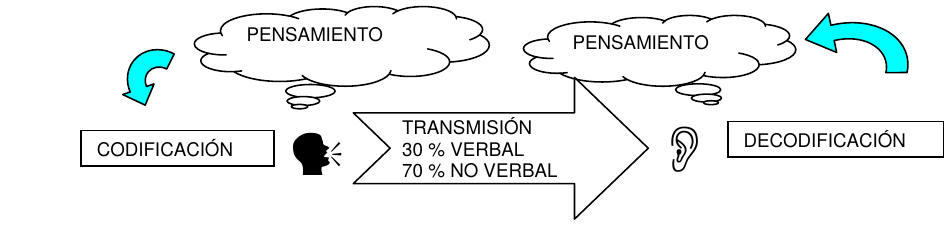
\includegraphics[width=0.97\linewidth]{figuras/fig_p042_19.png}
\end{center}

Desarrollar una idea es el paso más importante y el primero para entablar una comunicación. Codificar consiste en cifrar el mensaje en palabras, gráficos, u otros símbolos adecuados para el canal a utilizar.

Transmisión, una vez desarrollado el mensaje se transmite con el método elegido, el emisor selecciona el canal de comunicación y el momento oportuno para entablar la comunicación. Debe cuidar que el canal elegido no tenga barreras ni interferencias, teniendo así mayores posibilidades de llegar al receptor y captar su atención.

Recepción: Si el receptor no recibe en tiempo y forma el mensaje este se pierde.

Descodificación: El mensaje es descifrado para ser entendido. No basta con dar una orden o decir algo para que se efectúe la comunicación ya que esta no se establece si el receptor no entiende el mensaje. Es el receptor quien decide si comprende o no el mensaje.

Aceptación: Una vez que el receptor a recibido y decodificado el mensaje, tiene la oportunidad de aceptarlo o rechazarlo. La aceptación depende de una decisión personal y admite grados, de manera tal que el receptor tiene mucho control sobre la aceptación de todo el mensaje o solo en algunas partes. Algunos factores que influyen sobre la decisión giran en torno a las percepciones de la exactitud del mensaje, la autoridad del emisor, y las implicaciones que tiene en el comportamiento del receptor.

Uso: El receptor puede rechazar la información, efectuar la tarea siguiendo las instrucciones, guardarla para el futuro u optar por otra alternativa. Se trata de un paso decisivo de acción, y en gran medida el receptor puede determinar qué hacer con él.

Retroalimentación: Cuando el receptor reconoce el mensaje y responde al emisor, o acciona, la retroalimentación ha tenido lugar y esto cierra el lazo de comunicación, esta etapa tiene gran importancia para que el emisor establezca si la el mensaje fue entendido correctamente.


% ---- página 43 ----

\begin{center}
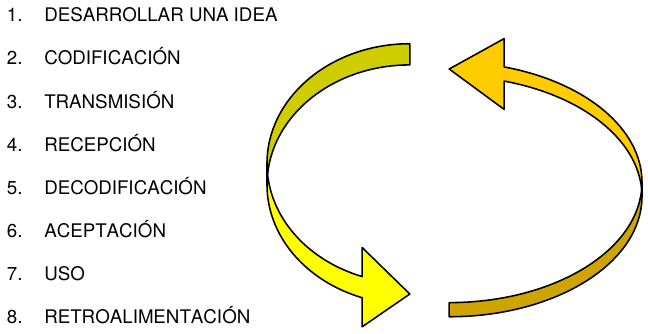
\includegraphics[width=0.66\linewidth]{figuras/fig_p043_20.png}
\end{center}

\subsubsection*{ACTIVIDAD}
Lea la siguiente conversación y responda el cuestionario que le sigue:

A: Autorizado descenso para 2-5 hasta 300 metros, notifique para final.

B: Descenso para 2-5 hasta 300, notificare final. ¿Me informa el QNH local?

A: Presión 1012 milibares, viento de los 120 a 30 Km. por hora, visibilidad buena.

B: (Dos sonidos cortos) ........................................

A: Para final de 2-5.

B: Autorizado final, y aterrizaje, notifique aterrizado.

A: Notificare aterrizado.

Responder:

1- ¿Entre quienes se realiza la comunicación?

2- ¿Qué canal de comunicación utilizan?

3- ¿Entiende el código utilizado?

4- ¿Qué se están comunicando?

5- ¿Hay retroalimentación?

\subsubsection*{CLASIFICACIÓN}
Las comunicaciones, en general, pueden ser clasificadas en:

Graficas: Son todos los tipos de comunicación en el que se utiliza símbolos gráficos como el alfabeto o símbolos. Dentro de este grupo tenemos la publicidad, los periódicos, manuales, textos, cartas, memorando, e-mail, mensajes de texto, carteles, recetas, los carteles de transito, la publicidad grafica, el código Morse, sistema de banderas utilizado en navegación, etc.

\begin{itemize}
  \item 
\end{itemize}

% ---- página 44 ----

Verbales: Son todos los tipos de comunicación en el que el mensaje es transmitido mediante sonidos verbales, dentro de este grupo encontramos, los discursos, las clases, las conversaciones, las reuniones, las canciones, la radio, etc.

Corporales: Son todos los tipos de comunicación en el que el mensaje es transmitido mediante movimientos corporales como el lenguaje de los sordomudos, danzas, sistema de señales entre los señaleros de una empresa aérea con los pilotos de aeronaves durante las maniobras de estacionamiento, etc.

También podemos clasificar las comunicaciones según sean:

Intencionales: Que son aquellas, como su nombre lo indica, que se hacen intencionalmente, sean ellas escritas, verbales, por señales u otros medios, y No intencionales: Son las que, también como su nombre lo sugiere, no se tuvo la intención de transmitir, pero, que sin embargo, se emiten. Por ejemplo: La vestimenta, el rubor, el temblor de las manos, el color tostado de la piel, etc. Muchas veces estas comunicaciones no intencionales no se las desean hacer, se las trata de ocultar, pero, a un observador perspicaz no se le pueden escapar y le sirven para obtener datos de su interlocutor confirmando o negando lo que intencionalmente éste le está comunicando. De ahí su utilidad en la actividad profesional como aseverativas o negativas de lo que se nos comunica intencionalmente.

\subsubsection*{INTERFERENCIAS EN LA COMUNICACIÓN}
Son hechos o acciones que actúan como barreras y dificultan la comunicación o que impiden por completo su recepción. Se las puede clasificar en dos categorías.

\begin{itemize}
  \item Interferencias físicas: Son las originadas en el mundo externo que nos rodea, por ejemplo: El ruido, el corte de energía eléctrica, la descompostura del aparato emisor o receptor, etc.
  \item Interferencias psíquicas: Son denominadas así porque acontecen en el mundo interno, en la psiquis del individuo, por ejemplo: La antipatía que siente el receptor hacia quien emite; desigualdad de interpretación de la simbología utilizada en el mensaje, distracciones, la falta de interés de éste en el tema, interpretación más que comprensión y otras que se encuentran en la figura siguiente.
\end{itemize}

\begin{center}
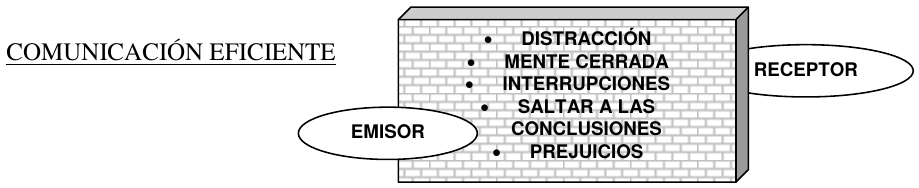
\includegraphics[width=0.94\linewidth]{figuras/fig_p044_21.png}
\end{center}

\begin{itemize}
  \item CÓDIGO EN COMÚN
  \item MARCO DE REFERENCIA DEL OTRO
  \item INCONDICIONAL ATENCIÓN AL OTRO
  \item NO INTERRUMPIR HASTA FINALIZAR LA IDEA
  \item SINCRONIZAR LOS TIEMPOS
  \item CONCENTRACIÓN
  \item LIBERTAD DE EXPRESIÓN
  \item EVITAR DISTRACCIONES
  \item EVITAR LAS INTERFERENCIAS EN EL CANAL
\end{itemize}

% ---- página 45 ----

\subsubsection*{COMUNICACIÓN EN LAS ORGANIZACIONES}
Por la línea de mando, en forma ascendente se transmite información al superior que de esta forma se entera del progreso del trabajo y de los sucesos más significativos. Sin embargo, esta línea no es el conducto de comunicación sencillo y directo que con frecuencia se supone. Existen ciertas peculiaridades que afectan la calidad, velocidad y exactitud de la transmisión de información en forma verbal. En las comunicaciones hacia abajo, de superiores a subalternos, a causa de la extrema sensibilidad hacia el superior, los subalternos intentan constantemente anticiparse a los deseos del jefe procurando interpretar cada uno de los gestos y palabras de este, el jefe no necesita expresar con palabras sus ideas o lo que espera de la tarea, esto ocasiona interpretaciones erróneas y confusiones. En las comunicaciones hacia arriba los subalternos siempre dicen lo que los jefes quieren escuchar y censuran y falsean la información de las tareas que han salido mal o no han sido hechas. Se dan por supuestas que cada uno cumple con su tarea y no se tienen que notificar malas noticias, hay que dar la impresión que se está ejecutando correctamente las tareas, en consecuencia no conviene comentarle al jefe que el trabajo salió mal, esto genera en los jefes desinformación e imprecisiones sobre lo que ocurre en el avance del trabajo, lo que se transmite con las mismas censuras en forma ascendente a lo largo de cada escalón jerárquico, cada individuo situado en la línea de comunicación actúa como un filtro hasta el jefe supremo quien recibe algunos indicios de lo que ocurre luego de transcurridos algún tiempo desde el hecho.

El medio de comunicación escrito se transmite en forma de cartas, memorándums, informes, fichas, instrucciones, notas, ordenes de trabajo, o cualquier nombre que se disponga. Por lo común las organizaciones establecen el formato, estilo de redacción, tamaño de papel, tipo de letra, logotipos, encabezados, etc., de estas comunicaciones escritas, y desempeñan una función importante en el proceso total. Cada organización determina qué clase de comunicaciones deben ser escrita y cuales pueden realizarse en forma verbal, la comunicación escrita tiene la ventaja de quedar registrada y puede ser consultada, también constituye un registro legal exigido en ciertas organizaciones, como las que realizan actividades aeronáuticas, judiciales, médicas, etc. que por su actividad pueden ser utilizados como probatorios de las responsabilidades, en general, casi todas las comunicaciones en forma descendente es escrita, pero la comunicación se hace lenta y exige demasiado tiempo comparado con la comunicación verbal.

Dentro de toda organización hay también una gran cantidad de la que puede ser llamada “comunicación irregular” o informal, que no siguen los canales administrativos, ni ninguno de los patrones formales prescriptos, que fundamentalmente se refiere a las relaciones humanas en la situación del trabajo y que sirve a las necesidades de la gente más bien que a las del trabajo. Esta información se llama comúnmente rumores, habladillas o chismes, deducciones, especulaciones, y constituyen en la mayoría de las organizaciones un aspecto aceptado, tienen una gran velocidad de transmisión, poca precisión, y se distorsiona cada vez que se transmite.


% ---- página 46 ----

\subsubsection*{LA ORGANIZACIÓN NO PUEDE EXISTIR SIN LA COMUNICACIÓN}

\begin{center}
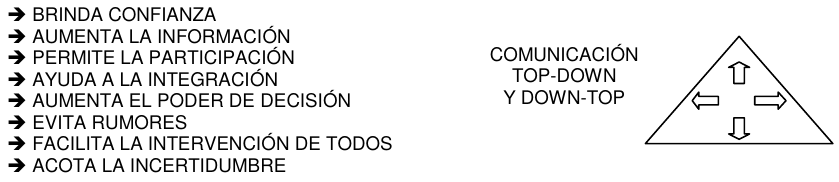
\includegraphics[width=0.86\linewidth]{figuras/fig_p046_22.png}
\end{center}

\subsection*{ADVERTENCIA}
\begin{itemize}
  \item NO SE PUEDE ESCUCHAR SI SE ESTA HABLANDO
  \item UNA PERSONA IRRITADA SIEMPRE DA UN SIGNIFICADO ERRÓNEO A LAS PALABRAS
  \item LA SUSPICACIA Y LA FALTA DE ACEPTACIÓN AL EMISOR DIFICULTA LA COMUNICACIÓN
  \item NO PRESTAR ATENCIÓN AL HABLANTE ES UNA FALTA DE EDUCACIÓN HACIA EL EMISOR
  \item ESTABLECER CONJETURAS O PREJUICIOS CONTAMINA EL MENSAJE
  \item NO DISPONER DEL TIEMPO NECESARIO PARA ESCUCHAR FRACTURA EL MENSAJE
  \item NO DISPONER DEL ESPACIO ADECUADO MUTILA LA COMUNICACIÓN
  \item LA FALTA DE CONCENTRACIÓN PIERDE TRAMOS DEL MENSAJE
  \item FALTA DE DISPOSICIÓN DE UN CÓDIGO COMÚN GENERA MALAS INTERPRETACIONES
  \item HABLAR MUCHO Y ESCUCHAR POCO O NADA ES UN MONOLOGO
  \item EL TRATO CON ALTIVEZ CENSURA AL INTERLOCUTOR
  \item FALTA Y/O AUSENCIA DE ALGÚN ELEMENTO DE COMUNICACIÓN HACE FRACASAR LA COMUNICACIÓN
\end{itemize}
Lectura recomendada

\subsubsection*{LOS FACTORES HUMANOS Y LA CALIDAD DEL MANTENIMIENTO AERONÁUTICO}
En la actividad aeronáutica, el factor humano tiene un rol decisivo en la generación de los \textbf{incidentes y} \textbf{accidentes de aviación}. Se estima que todos los accidentes en la industria de la aviación son causados, en un 20\% por la maquinaria, (mala manufactura de una parte o pieza de un equipo), \textbf{y en un} \textbf{80\% por factores humanos}. Como expresa \textbf{Clif Stroud, }editor de la prestigiosa revista Aviation Maintenance en su edición de febrero de 1997: "Uno de los tópicos más candentes de discusión en el ámbito de mantenimiento, en este preciso momento, es el factor humano". "El común denominador en todos los incidentes y accidentes, es el ser humano -la parte falible del proceso de toma de decisiones". "Y toda la atención que por años había estado focalizada sobre los Pilotos y como ellos tomaban las decisiones, está finalmente empezando a desplazarse hacia los Técnicos; y era hora". Esto mismo es ratificado, por \textbf{John Goglia, un Técnico de Mantenimiento de Aeronaves }-ex USAir-, reconocido experto internacional, y actualmente designado Presidente del Comité Directivo de la National Transportation Safety Board (NTSB) de USA, en el mismo número de la mencionada revista: "Los Pilotos tienen 25 años o más de ventaja en investigación sobre factores humanos. Me han dicho que para los tripulantes comenzó en 1940. Y aquí estamos en Mantenimiento, en los '90s, y recién comenzamos". Por su parte John F. Gorsuch, Editor Asociado de Aviation Maintenance, opina: "Los componentes de las aeronaves y los métodos de trabajo, han mejorado constantemente por la experiencia y la nueva tecnología; pero el factor de error humano se ha incrementado significativamente. Mediante fuertes esfuerzos cooperativos, estas áreas de problemas están siendo rápidamente identificadas y tratadas de solucionar a través de la investigación. La NTSB, trabajando conjuntamente con las aerolíneas y los sindicatos, está progresando en la causa de los factores humanos en el ámbito de Mantenimiento. Los resultados han sido buenos."

Los factores humanos más comunes que contribuyen a que se produzcan errores son los siguientes: \textbf{Falta de comunicación interna entre los mismos integrantes del grupo técnico; desidia; falta de} \textbf{capacitación; stress; distracción; mal desarrollo del trabajo en equipo; fatiga por excesiva} \textbf{cantidad de horas de trabajo; y por último, falta de conciencia por parte de las empresas y del}


% ---- página 47 ----

\textbf{personal, sobre la variedad de factores humanos que inciden en la calidad del trabajo de} \textbf{mantenimiento, y que a su vez afectan la seguridad en vuelo.}

Por eso es indispensable, un entrenamiento apropiado para el personal técnico aeronáutico en factores humanos. Sobre esa serie de errores -también conocida como cadena de eventos-, cuya existencia previa es la que posibilita que un accidente aéreo suceda.

\textit{Este es un extracto del articulo Los Factores Humanos y la Calidad del Mantenimiento Aeronáutico} \textit{escrito por William Johnson, PhD de la FAA, escrito en la revista Aviation Maintenance (04/97).}

\section*{LA CULTURA ORGANIZACIONAL}
La cultura de las organizaciones implica una filosofía que incluye valores, creencias, principios motivaciones, actitudes, deseos, historia, objetivos, tradiciones, suposiciones, éxitos, fracasos, experiencias, miedos, que son compartidos por todos los miembros por tener un significado común para ellos, esta cultura dará origen a la personalidad de la organización, al igual que forma la personalidad de los individuos.


\begin{recuadro}
\textbf{La Cultura Organizacional es el modo de pensar colectivo de una Organización basado} \textbf{en un conjunto de valores, creencia, objetivos, etc., compartidos por los integrantes de la} \textbf{Organización.}
\end{recuadro}

Existen organizaciones ricas en tradiciones, valores y creencias, con lo que se logran la solidez de la empresa. Los fundadores de las empresas cumplen un rol preponderante en este sostenimiento, son los iniciadores de un sistema cultural. A lo largo de los años la personalidad de los fundadores otorga su propio sello a las empresas. También ocurre en las empresas familiares medianas en donde el dueño o el gerente, con personalidad fuerte, impone ciertas características particulares a la cultura de la organización. Existe una relación entre la personalidad de los que ejercen el gobierno, la estructura, la cultura de la organización y la estrategia seguida.

Cada organización se distingue de las demás por su cultura así como una sociedad se distingue por poseer una determinada cultura que la compone, hay varios elementos que se combinan para dar origen a una cultura y en la medida que estos elementos se combinen surgirán las diferentes características de las organizaciones. Estos elementos son:

LA GENTE Cada organización incorpora gente de distintas fuentes, la gente es diversa, llegan a la organización con diversas creencias acerca de cómo se hacen las cosas y diversos hábitos de pensamiento.

LA HISTORIA Cada organización tiene su historia y esta historia está llena de fracasos y éxitos, Cada éxito o fracaso deja una huella, un trazo distintivo, un hábito, una institución, una creencia. EL LIDERAZGO El liderazgo es crítico, en aviación particularmente, es el nivel superior el que fija las reglas en el área de seguridad.

EL ENTORNO Los entornos son muy diversos, para una aerolínea por ejemplo, incluye la meteorología, la macroeconomía, políticas gubernamentales, tipos de pasajeros que transporta, tecnología utilizada.


% ---- página 48 ----

Dependiendo como se pongan en juego estos elementos obtendremos las diferentes culturas organizacionales, pueden ser más o menos flexibles, innovadoras o conservadoras, atentas a las necesidades de sus miembros o de los clientes reales y potenciales o cerradas a las demandas, tolerantes al conflicto, con identidad, autónoma, con valoración de la tarea del personal. En el cuadro siguiente se muestra cinco características de las culturas organizaciones. Para que una organización sea saludable debería tener una mezcla de los diferentes tipos de personalidades:


\begin{center}
\small
\begin{tabular}{|p{\dimexpr0.210\linewidth-2\tabcolsep\relax}|p{\dimexpr0.180\linewidth-2\tabcolsep\relax}|p{\dimexpr0.609\linewidth-2\tabcolsep\relax}|}
\hline
ORGANIZACIÓN & CULTURA & CARACTERÍSTICA \\ \hline
PARANOICA & PARANOICA & La empresa está plagada de sospechas, desconfianza, búsqueda de enemigos en el entorno, baja motivación, percepciones uniformes pero distorsionadas, uso de la información como fuente de poder. \\ \hline
DEPRESIVA & EVASIVA & La empresa no tiene iniciativa, los gerentes no están motivados, demoras y fobias a tomar decisiones, pasividad. \\ \hline
DRAMÁTICA & CARISMÁTICA & La cultura organizacional está caracterizada por subordinados dependientes que idealizan al líder, lo creen infalible y nunca lo cuestionan, hay una entusiasta adhesión a las creencias y objetivos del número uno. \\ \hline
COMPULSIVA & BUROCRÁTICA & Organización burocrática, jerárquica, rígida, orientadas a reglas, centralizada y orientada hacia adentro, abundan los procedimientos rutinarios. \\ \hline
ESQUIZOIDE & POLITIZADA & El vacío de liderazgo es llenado por jugadores politizados que compiten por poder y posición. Se descuida la cooperación y coordinación. \\ \hline
\end{tabular}
\end{center}

\section*{CAMBIO Y RESISTENCIA AL CAMBIO}
El termino cambio, referido a lo organizacional, se refiere a cualquier alteración que ocurre en el ambiente de trabajo, en la estructura orgánica, las funciones, producto elaborado, horarios, salarios, ubicación de la planta, dirección, procesos de producción, misión, nuevas maquinarias, reingenierías, etc.

Estas son algunas de las expresiones verbales más comunes que se encuentran y que sirven de alerta cuando estamos frente a la resistencia al cambio.

\textbf{\textit{“¿De qué problema me hablan? Aquí las cosas se arreglan solas. Hay que darle tiempo al}} \textbf{\textit{tiempo y todo se pondrá en su lugar” “Aquí no hay ningún problema, son inventos de los jefes}} \textbf{\textit{para justificar el cargo” “Siempre lo hicimos así” “Hay gente que tiene la manía de buscarle}} \textbf{\textit{la quinta pata al gato. Encuentran problemas donde no los hay” “Esto no va a funcionar”}} \textbf{\textit{“Antes era más fácil”.}}

La introducción de cambios, y aun de simples proyectos de innovación, provocan al comienzo resistencia, ello se produce cuando se trata de modificar ciertos hábitos cotidianos o de promover nuevos métodos de trabajos o de organización. La transición resulta siempre difícil. Todo el sistema social de una organización tiende a mantenerse en estado de equilibrio hasta que la presión de cambios inevitables obliga a una readaptación. Es decir, en cuanto un grupo de trabajadores de una empresa ha conseguido adoptar un patrón de comportamiento más o menos afortunado respecto a las relaciones mutuas y el ajuste al trabajo, tienden a resistirse a cualquier cambio que pueda modificarlo. Esto tiene su contrapartida en la personalidad individual. Cada individuo tiende a manifestar un tipo de conducta constante, que constituye lo que llamamos su personalidad, y perdura más o menos invariable a lo largo de toda su vida, puede sufrir


% ---- página 49 ----

influencias, si se ve obligado a ello, pero siempre adaptándolas previamente al esquema establecido.

También los sistemas sociales aceptan con dificultad los cambios, si son demasiado radicales, el grupo social no puede asimilarlos a su patrón de conducta y actitudes, y experimenta una profunda sensación de inseguridad, ansiedad e incluso hostilidad, que se traduce en sentimientos de frustración y desmoralización.

Nuestra vida cotidiana está regida por un conjunto de costumbres, hábitos, modelos, de esta forma la resistencia al cambio puede provenir:

\begin{itemize}
  \item Del carácter coercitivo que con frecuencia estos tienen (no nos consultaron o informaron).
  \item Estados de fatiga y la edad influyen en la respuesta al cambio.
  \item El temor al fracaso o al bajo rendimiento o la pérdida de prestigio.
  \item De la necesidad de seguridad traducido como la preferencia por lo conocido antes que lo desconocido.
  \item De los intereses particulares que podrían verse amenazados.
  \item De la falta de visión y claridad respecto a los eventuales beneficios del cambio.
  \item De la inercia que hace preferible mantener un mismo ritmo antes que hacer un esfuerzo adicional por cambiarlo.
  \item De interpretaciones contradictorias respecto al cambio, sus alcances, objetivos, etc.
  \item De la falta de recursos, que pueden hacer difícil o imposible mantener una innovación.
  \item De envidias y malas disposiciones internas que hacen que personas y áreas de una organización se opongan a innovaciones provenientes de otras personas o áreas.
\end{itemize}
Se han descubierto importantes factores psicosociales de la resistencia al cambio y ciertos medios de reducirla. En muchos casos el reforzamiento de la información y la proposición de ciertas formas de participación en el cambio encuentran adhesión, pero no siempre es así.

Hay dos postulados en relación al comportamiento de los grupos: Todos los hombres tienen siempre deseo de participar si los dueños de la autoridad adoptan métodos más cooperativos y permisivos, los subordinados responden siempre. Por ejemplo los cambios son pocas veces propuestos en forma espontánea e incondicional por los dueños de la información y del poder, quienes deben abandonar una especie de zona reservada, susceptible de transformar en mayor o menor medida al propio sistema del poder. (Los trabajadores invitados a colaborar pueden poner en duda tanto los métodos de trabajo como la política de la empresa y los subordinados temen que si ceden pueden perder cierta autonomía respecto a la dirección).

\subsubsection*{FORMAS DE RESISTENCIA AL CAMBIO}
Se consideran como formas de resistencia “Todas aquellas expresiones visibles u observables, indirectas, conscientes o inconscientes de resistencia, que esconden una causa verdadera no expresada por los individuos de una organización ante un cambio, por una auto imposición, por la falta de mecanismos que permitan la libre expresión de los miembros de una organización, por imposición expresa de la organización”.

El cuadro muestra las diferentes formas de resistencia:


% ---- página 50 ----

\begin{center}
\small
\begin{tabular}{|p{\dimexpr0.007\linewidth-2\tabcolsep\relax}|p{\dimexpr0.235\linewidth-2\tabcolsep\relax}|p{\dimexpr0.007\linewidth-2\tabcolsep\relax}|p{\dimexpr0.007\linewidth-2\tabcolsep\relax}|p{\dimexpr0.235\linewidth-2\tabcolsep\relax}|p{\dimexpr0.008\linewidth-2\tabcolsep\relax}|p{\dimexpr0.007\linewidth-2\tabcolsep\relax}|p{\dimexpr0.235\linewidth-2\tabcolsep\relax}|p{\dimexpr0.007\linewidth-2\tabcolsep\relax}|p{\dimexpr0.007\linewidth-2\tabcolsep\relax}|p{\dimexpr0.235\linewidth-2\tabcolsep\relax}|p{\dimexpr0.008\linewidth-2\tabcolsep\relax}|}
\hline
 & ACEPTACIÓN &  &  & INDIFERENCIA &  &  & RESISTENCIA PASIVA &  &  & RESISTENCIA ACTIVA &  \\ \hline
\multicolumn{3}{|p{\dimexpr0.250\linewidth-2\tabcolsep\relax}|}{ENTUSIASMO} & \multicolumn{3}{|p{\dimexpr0.250\linewidth-2\tabcolsep\relax}|}{APATÍA} & \multicolumn{3}{|p{\dimexpr0.250\linewidth-2\tabcolsep\relax}|}{RESISTENCIA AL APRENDIZAJE} & \multicolumn{3}{|p{\dimexpr0.250\linewidth-2\tabcolsep\relax}|}{TRABAJO A RITMO LENTO} \\ \hline
\multicolumn{3}{|p{\dimexpr0.250\linewidth-2\tabcolsep\relax}|}{COOPERACIÓN} & \multicolumn{3}{|p{\dimexpr0.250\linewidth-2\tabcolsep\relax}|}{PÉRDIDA DE INTERÉS EN EL TRABAJO} & \multicolumn{3}{|p{\dimexpr0.250\linewidth-2\tabcolsep\relax}|}{PROTESTAS} & \multicolumn{3}{|p{\dimexpr0.250\linewidth-2\tabcolsep\relax}|}{AUSENCIA} \\ \hline
\multicolumn{3}{|p{\dimexpr0.250\linewidth-2\tabcolsep\relax}|}{COOPERACIÓN BAJO PRESIÓN DE LA DIRECCIÓN} & \multicolumn{3}{|p{\dimexpr0.250\linewidth-2\tabcolsep\relax}|}{OBEDIENCIA SOLO A LAS INSTRUCCIONES} & \multicolumn{3}{|p{\dimexpr0.250\linewidth-2\tabcolsep\relax}|}{RESPETO DESMEDIDO AL PROCEDIMIENTO} & \multicolumn{3}{|p{\dimexpr0.250\linewidth-2\tabcolsep\relax}|}{NO PARTICIPACIÓN} \\ \hline
\multicolumn{3}{|p{\dimexpr0.250\linewidth-2\tabcolsep\relax}|}{RESIGNACIÓN PASIVA} & \multicolumn{3}{|p{\dimexpr0.250\linewidth-2\tabcolsep\relax}|}{CONDUCTA REGRESIVA} & \multicolumn{3}{|p{\dimexpr0.250\linewidth-2\tabcolsep\relax}|}{TRABAJO EN SU MÍNIMA EXPRESIÓN} & \multicolumn{3}{|p{\dimexpr0.250\linewidth-2\tabcolsep\relax}|}{ERRORES REITERADOS} \\ \hline
\multicolumn{3}{|p{\dimexpr0.250\linewidth-2\tabcolsep\relax}|}{INDIFERENCIA} & \multicolumn{3}{|p{\dimexpr0.250\linewidth-2\tabcolsep\relax}|}{---} & \multicolumn{3}{|p{\dimexpr0.250\linewidth-2\tabcolsep\relax}|}{---} & \multicolumn{3}{|p{\dimexpr0.250\linewidth-2\tabcolsep\relax}|}{SABOTAJE DELIBERADO} \\ \hline
\end{tabular}
\end{center}

Esto muestra que la resistencia puede ser tan sutil como la resignación pasiva y tan potente como el sabotaje deliberado. Los jefes deben ser capaces de reconocer las formas de resistencia al cambio tanto en sí mismos como en los demás, si pretenden ser eficientes en generar y apoyar el cambio.

Lectura Recomendada

\subsubsection*{LA CULTURA ORGANIZACIONAL}
Es relevante hablar de cultura organizacional, sólo si pensamos en la organización como un sistema-entorno. Cualquier sistema es dependiente o codependiente de un entorno que en una síntesis mayor configura otro sistema. Se debe señalar que en toda relación entre un sistema y su entorno existe una coherencia básica, por cuanto el primero extrae gran parte de sus características del segundo, concretamente la cultura organizacional extrae parte importante de sus premisas de la sociedad en la que la organización se encuentra.

La cultura organizacional se refiere a las presunciones y creencias básicas compartidas por los miembros de la organización (Edgar Shein). Estas creencias operan de manera inconsciente definiendo la visión que los miembros de la organización tienen de ella y de sus relaciones con el entorno; y han sido aprendidas como respuestas a los problemas de subsistencia en el entorno y a los propios de la integración interna de la organización.

Es así que la cultura organizacional es el conjunto de premisas básicas sobre las que se construye el decidir organizacional. Como la cultura organizacional permanece invisible para los miembros de una organización (no son conscientes), dejan de ser vistas en su carácter contingente (de la vida cotidiana) y permiten configurar el mundo de tal manera que visto a través de ellas y con su ayuda, el mundo aparece como si fuera de un cierto modo, sin percatarse o darnos cuenta que es la cultura la que lo está haciendo perfilarse así. Cuando abandonamos la ilusión de que el mundo está compuesto por fuerzas separadas, desconectadas y que actúan con total independencia, podemos comenzar a construir “organizaciones que aprenden” (Peter M Senge, La Quinta Disciplina) Uno ve lo que dibuja y dibuja lo que ve, no otra cosa. Los seres humanos y las organizaciones que describimos son sistema autorreferentes, es decir, todo aquello que utilizan del entorno tiene relación con supervivencia y adopción básica del sistema que la recibe y por otro lado, la capacidad de percibir señales del entorno no depende del entorno, sino con el sistema que percibe con lo cual de nuevo la referencia vuelve al sistema u organización desde el cual se genera la necesidad.


% ---- página 51 ----

Nunca una organización se encuentra desadaptada de su entorno, pues en ese momento muere. Lo que ocurre es que este funcionamiento en los niveles umbrales de supervivencia que muestran una cierta estabilidad, pero no necesariamente un desarrollo. De esta manera las premisas que conducen los destinos de una organización se establecen y rigidizan, sin necesariamente ser fruto de una decisión consciente. Las organizaciones “son como son” y los miembros de la organización difícilmente pueden imaginar que pudieran ser o haber sido de otra manera o forma. Es comprensible entonces que el intento de cambio de una cultura determinada no es asunto de implantar un nuevo modelo cultural, sino conducirlo a través de un proceso de cambio planificado. De esta manera, se vuelve relevante la perspectiva de la organización que aprende. La era actual, considerada la era del conocimiento, impondrá un cambio continuo sobre las organizaciones en orden a que éstas mejoran la conformidad de la calidad del producto-servicio.

\textit{Este artículo forma parte de la serie de contenidos dedicados al concepto: Organizaciones} \textit{Scouts abiertas al aprendizaje. Para su mejor comprensión, recomendamos leer los fascículos} \textit{editados por la Red de Desarrollo Institucional}

\subsubsection*{CUESTIONARIO 4}
1. ¿Qué son las relaciones humanas?, ¿en qué ciencias se apoya?, ¿qué objetivo persigue?

2. ¿Cuál es el nuevo concepto de estructura tratado en esta parte?

3. ¿Cómo se definen a los grupos?

4. ¿Cuáles son las fuentes de autoridad informales dentro del grupo?

5. ¿Cuáles son las ventajas de las comunicaciones escritas frente a las verbales?

6. ¿Cuáles son los símbolos de posición en las estructuras informales? Mencionar ejemplos.

7. ¿Qué condición debería reunir una organización laboral para que sea satisfactoria?

8. ¿Cómo se clasifican las interferencias en la comunicación?

9. ¿Cómo se establece la posición informal de un individuo en una organización?

10. ¿Qué es el poder y cuáles son sus bases?

11. ¿Cuáles son las barreras de la comunicación?

12. ¿Por qué se produce resistencia a los cambios?

13. ¿La participación puede reducir la resistencia al cambio?

14. ¿Quiénes son más resistentes al cambio los jóvenes o los adultos?

15. ¿Por qué hay que cambiar?

16. ¿Cuáles son los factores que impulsan los cambios?


% ---- página 52 ----

\subsubsection*{CONTENIDOS DEL NÚCLEO TEMÁTICO CUARTO}
La economía, concepto. La economía como ciencia social, clasificación. Los agentes económicos. Factores de la producción. El problema económico .Retribución de los factores. Mercados: Oferta y Demanda, precio. Teoría del Valor. Costo: concepto, clasificación, ejemplos, Análisis de Mercado.

\section*{ECONOMÍA}
\subsubsection*{INTRODUCCIÓN}
La Economía se ocupa de las cuestiones que surgen en relación con la satisfacción de las necesidades de los individuos y de la sociedad. La satisfacción de las necesidades materiales (alimentos, vestido, o vivienda) y no materiales (educación, diversión) de una sociedad obliga a sus miembros a llevar a cabo determinadas actividades productivas. Mediante estas actividades se obtienen los bienes y servicios que necesita la sociedad.

La economía se preocupa de la manera en que se administran recursos escasos, con objeto de producir diversos bienes y distribuirlos para su consumo entre los miembros de la sociedad.

Frente a todos los problemas que se plantean a los individuos y a las organizaciones, lo que pretende la Economía es ofrecer un método para ordenar y establecer las prioridades a la hora de tomar decisiones sobre las necesidades individuales o colectivas que se desean satisfacer, debido a que los recursos para satisfacer las necesidades son limitados.

La ciencia económica no pretende ofrecer recetas exactas para resolver los problemas económicos, pues siempre habrá elementos arbitrarios en el comportamiento de los individuos. LA ECONOMÍA COMO CIENCIA La comprensión del funcionamiento de la economía exige contar con teorías que expliquen el funcionamiento de los fenómenos económicos. La teoría económica provee una estructura lógica para organizar y analizar datos económicos, poner en orden las observaciones de los hechos económicos, con el fin de explicar de qué manera están relacionados.

Para simplificar el análisis se utilizan modelos económicos, que son aproximaciones a la realidad, a través de supuestos, argumentos y conclusiones que explican una determinada proposición o un aspecto de un fenómeno más amplio.

El objeto principal de estudio de los modelos es el hombre, y este es libre y no esta sujeto a leyes inflexibles. Este hecho no solo dificulta la investigación en Economía, sino también la modelización de los fenómenos económicos. Afortunadamente las predicciones con éxito del comportamiento de los grupos humanos son factibles gracias a la denominada “La Ley de los Grandes Números”, que establece que una gran mayoría de individuos tiene un comportamiento predecible con gran certeza, y que los que no lo tienen se compensas anulándose sus efectos.

\subsubsection*{CONCEPTO}

\begin{recuadro}
\textbf{Economía es la ciencia que estudia la asignación más conveniente de los recursos escasos} \textbf{de una sociedad para la obtención de un conjunto ordenado de objetivos.}
\end{recuadro}

La economía no estudia un área o un campo de la actividad humana, sino un aspecto de esta: El aspecto de toda actividad humana que, en el intento de satisfacer las necesidades materiales, implica la necesidad de elegir.


% ---- página 53 ----

\subsubsection*{MACROECONOMÍA Y MICROECONOMÍA}
El análisis económico tiene lugar bajo dos enfoques diferentes:

La macroeconomía busca la imagen que muestre el funcionamiento de la economía en su conjunto. Su propósito es obtener una visión simplificada del funcionamiento de la economía, pero que al mismo tiempo permita conocer y actuar sobre el nivel de la actividad económica de un país determinado o de un conjunto de países. Cuando se trata de agregados, o sea, cuerpos compuestos (un sector productivo, una región geográfica, la economía de un país, etc.) el tema se enfoca desde el punto de vista macroeconómico, por ejemplo la inflación.

Cuando el objeto de análisis se ubica en el nivel de las unidades económicas (empresas, familias, mercado de un bien específico), el tema se encuadra dentro de la óptica microeconómica. La Microeconomía estudia los comportamientos básicos de los agentes económicos individuales. Como ejemplo pertenece a este campo los mecanismos de formación de los precios. Mientras en el campo de la microeconomía se trabaja con elementos relativamente homogéneos, en el ámbito de la macroeconomía coexisten partes homogéneas y heterogéneas, producto de la sumatoria de diversas unidades que observa ciertos elementos comunes.

La macroeconomía suministra un contexto de referencia a la microeconomía. Ejemplo: Para establecer la política salarial de una empresa metalúrgica, deberá tenerse en cuenta la estructura de ingresos del factor trabajo en ese sector; el estudio del costo de combustibles de una empresa no puede desligarse de la estructura energética de la región donde se encuentra.

Se debe remarcar que se trata de diferentes enfoques de estudio, un mismo elemento económico puede ser estudiado desde ambos puntos de vista.

\subsubsection*{LA POLÍTICA MACROECONÓMICA}
Está integrada por el conjunto de medidas gubernamentales destinadas a influir sobre la marcha de la economía en su conjunto. Los objetivos últimos de la política macroeconómica suelen ser:

\begin{itemize}
  \item La inflación.
  \item El desempleo.
  \item El crecimiento.
  \item La distribución.
  \item La estabilidad económica.
\end{itemize}
Junto a estos grandes objetivos, las autoridades administrativas también prestan especial atención al presupuesto público (déficit presupuestario) y a las cuentas con el sector exterior (balanza de pagos).

\subsubsection*{LAS NECESIDADES}
Es la sensación de carencia de algo unida al deseo de satisfacerla. Precisamente, esa sensación de carencia (necesidad), junto con las cosas o elementos (bienes y servicios) que utilizamos para satisfacerla y el esfuerzo que realizamos para obtenerlos (trabajo) constituyen los elementos básicos de la actividad económica. Desde el punto de vista de la economía, estas necesidades se pueden clasificar de la siguiente forma:


% ---- página 54 ----

\begin{center}
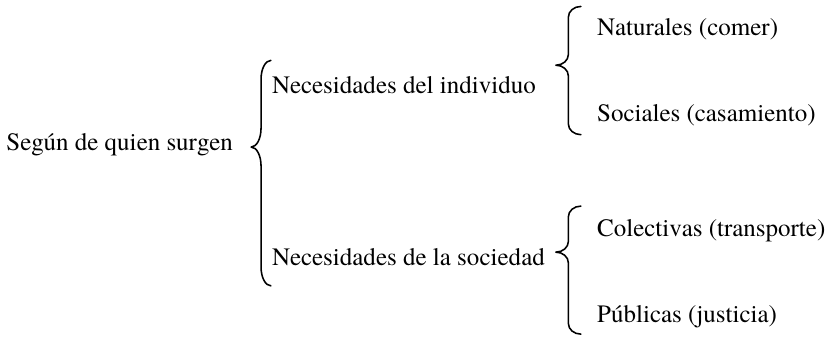
\includegraphics[width=0.86\linewidth]{figuras/fig_p054_23.png}
\end{center}

\begin{center}

\includegraphics[width=0.85\linewidth]{figuras/fig_p054_24.png}
\end{center}

\subsubsection*{PIRÁMIDE DE MASLOW}
Maslow en 1954 estableció que las necesidades humanas no tienen la misma fuerza, por lo general surgen con alguna prioridad.

\subsubsection*{JERARQUÍA DE LAS NECESIDADES}
La teoría de Maslow consideraba que las necesidades humanas básicas se podían organizar en orden de jerarquías y sostenía que las necesidades de orden más alto no se podían satisfacer a menos que se hubiesen satisfecho las de orden inferior.

El modelo propuesto parte del supuesto de que las personas buscan satisfacer sus necesidades más básicas (fisiológicas) antes de orientar su conducta hacia la satisfacción de las necesidades de nivel superior (autorrealización). Esta teoría supone que las necesidades de las personas dependen de lo que ya tienen.

Las necesidades humanas organizadas de acuerdo a su jerarquía de importancia son:

\begin{itemize}
  \item \textbf{Fisiológicas: }La necesidad de alimento, bebida, albergue y alivio del dolor.
  \item \textbf{Seguridad: }La necesidad de no sentirse amenazado, es decir, la ausencia de sucesos o ambientes amenazantes, protección contra daños materiales y emocionales.
  \item \textbf{De pertenencia, de interacción social y de amor generalizadas como necesidades} \textbf{sociales: }La necesidad de amistad, afiliación y pertenencia, interacción y amor.
  \item \textbf{Estima y Estatus: }La necesidad de autoestima y de ser estimado por los demás, autonomía y realización, posición social, reconocimiento y atención.
  \item \textbf{Autorrealización: }La necesidad de realizarse a sí mismo maximizando la utilización de capacidades, destrezas y aprovechamiento del potencial propio.
\end{itemize}
Como resultado de la jerarquización de las necesidades las personas se encuentran motivadas a cubrir las necesidades faltantes más que por preservar las ya cubiertas.


% ---- página 55 ----

\subsubsection*{LOS BIENES Y SERVICIOS}
Es todo medio capaz de satisfacer directa o indirectamente los deseos o necesidades tanto de los individuos como de la sociedad, que se encuentran disponibles para tal fin. Se pueden clasificar de la siguiente forma:


\begin{center}
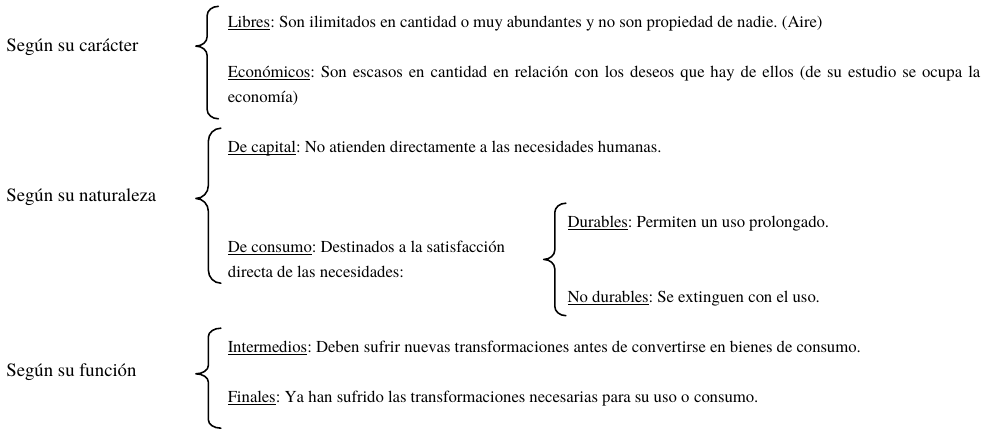
\includegraphics[width=1.00\linewidth]{figuras/fig_p055_25.png}
\end{center}

Si los bienes y servicios se encontraran en cantidades ilimitadas y listos para su inmediato consumo, la economía no tendría razón de existir. Pero, dado que el hombre debe dedicar su actividad a procurárselos con su esfuerzo, esta disciplina estudia su mejor aprovechamiento.

\subsubsection*{LOS AGENTES ECONÓMICOS}
En el desarrollo de las actividades económicas intervienen distintos protagonistas llamados agentes o actores económicos. La clasificación típica de los agentes económicos es la que distingue entre economías domesticas, empresas y sector publico.

Las economías domesticas: Las funciones de las economías domesticas consisten por un lado en consumir bienes y servicios, y por el otro, en ofrecer bienes y servicios de tal forma de proveerse de los recursos necesarios para satisfacer sus consumos. En un sentido amplio las economías domesticas son los individuos, familias, agrupaciones deportivas, culturales, asociaciones culturales o religiosas. Ellas pretenden maximizar la utilidad o satisfacción que obtienen en el consumo restringido por el presupuesto del que disponen. La parte del ingreso que no se consume, es destinado al ahorro. Usualmente a los bienes y servicios que las economías domesticas brindan se los suele llamar tierra, trabajo y capital.

La empresa: Realizan dos funciones básicas, por un lado, compran bienes y servicios en el mercado, y por otro lado transforman, elaboran y/o producen otros bienes y servicios y los venden en el mercado. Esta compra y venta la realizan guiadas por un objetivo: el de maximizar sus beneficios, es decir, la diferencia entre los ingresos por las ventas de los bienes y servicios y los costos de la adquisición de bienes y servicios para producirlos.

El sector publico: Integrado por el estado y sus instituciones, provee bienes y servicios, y redistribuye ingreso y riqueza. Los servicios más importantes provistos por el gobierno son las leyes y un mecanismo para su aplicación. Pero los gobiernos también proporcionan servicios


% ---- página 56 ----

como defensa nacional, tribunales, fuerzas policiales, salud pública, transporte, educación. Sus funciones fundamentales se pueden agrupar en las siguientes categorías: fiscales (impuestos), reguladoras, redistributivas (renta), estabilizadoras, y proveedoras de bienes y servicios públicos. Existen muchas teorías respecto al alcance del papel que debe desempeñar el estado en la actividad económica, como por ejemplo un garantizador del cumplimiento de los contratos privados, protectivo, liberal, exportador, etc. Los gobiernos adoptan el grado de participación acorde al objetivo que se han propuesto. La economía Política es el estudio del papel que debe desempeñar el estado en la actividad económica de los países.

\subsubsection*{LOS FACTORES PRODUCTIVOS}
Son los bienes y servicios empleados por las organizaciones en sus procesos de producción, todo lo que se utiliza para producir otros bienes y servicios. Estos bienes y servicios pueden ser adquiridos a las economías domesticas o a otras organizaciones. La clasificación tradicional de los factores productivos considera tres categorías:

Los recursos naturales: Nos referimos a todo lo que aporta la naturaleza al proceso productivo. Es decir la tierra utilizada por los agricultores o sobre las que se edifican las casa, las fabricas o las carreteras, los minerales como el cobre y el hierro, los recursos energéticos como petróleo y gas, este recurso se lo suele dividir entre recursos renovables a aquellos que se los puede utilizar reiteradamente y los no renovables a aquellos que se agotan al emplearlos en el proceso de producción.

El trabajo: Es el tiempo y las capacidades intelectuales que las personas dedican a las actividades productivas. Miles de ocupaciones y tareas a todos los niveles de calificación, la desempeñan los individuos, constituyendo el factor productivo esencial en cualquier sociedad avanzada. Se lo suele referir como capital humano entendiéndose por esta ultima denominación, la educación y formación profesional que incrementan el rendimiento del trabajo.

El capital: Lo forman los bienes durables de cualquier economía. Estos bienes son aquellos que no se destinan al consumo, sino que se emplean para producir otros bienes .En esta categoría se incluyen las maquinas, las edificaciones, las carreteras, las herramientas, las computadoras, los edificios, los camiones, etc.

Información: ¿?

\subsubsection*{LA ESCASEZ}
Todas las preguntas de la economía surgen de un sencillo e ineludible hecho: No siempre se puede obtener lo que uno quiere. Los deseos siempre exceden a los recursos disponibles para satisfacerlos. La escasez es un concepto relativo, en el sentido de que existe un deseo de adquirir una cantidad de bienes y servicios mayor que la disponible. Escasez no es equivalente que pobreza, la constante humana es que las necesidades son ilimitadas mientras que los recursos para obtenerla son limitados. La diferencia entre ambos es la escasez.

\subsection*{NECESIDADES (ILIMITADAS) – RECURSOS (LIMITADOS) = ESCASEZ}
El hecho de que los factores productivos estén disponibles en cantidades limitadas y que las necesidades humanas sean prácticamente ilimitadas plantea la inevitabilidad de elección. La necesidad de elegir se evidencia al considerar los tres problemas fundamentales a los que toda sociedad debe dar respuesta. ¿Qué producir? ¿Cómo producirlo? ¿Para quién?

Por ejemplo un niño quiere una gaseosa de 20 pesos y un paquete de caramelos de 15 pesos, pero sólo tiene un diez en el bolsillo. Un estudiante quiere ir a una fiesta el sábado por la noche pero


% ---- página 57 ----

también quiere terminar esa misma noche la tarea atrasada. El gobierno también afronta la escasez: El monto que quiere gastar en educación, defensa, salud, bienestar y otros servicios excede lo que recauda por impuestos. Los deseos simplemente no exceden a los recursos, los deseos no tienen límite.

\subsubsection*{LA ACTIVIDAD ECONÓMICA}
La actividad económica es lo que realizan los individuos y las organizaciones para afrontar la escasez. Y la economía es el estudio de cómo estos individuos y las organizaciones utilizan sus recursos limitados para tratar de satisfacer sus deseos ilimitados. Lo que produce las preguntas de la economía, es el hecho universal de la escasez:

\begin{itemize}
  \item Con recursos ilimitados no habría necesidad de idear mejores formas de producir bienes o servicios.
  \item Solamente haríamos lo que nos agradaría porque habría suficientes bienes y servicios para satisfacer a todo el mundo sin esfuerzo.
  \item El desempleo no sería un problema porque nadie trabajaría, con excepción de aquellos que quisieran trabajar por puro placer.
  \item No habría salarios.
  \item La inflación no sería un problema porque a nadie le importarían los precios.
  \item No habría necesidad de bienes provistos por el estado.
  \item Con una abundancia total, no existiría el comercio internacional, ya que no tendría sentido trasladar los bienes de un lugar a otro.
  \item No habría países pobres y ricos: Todos tendríamos tanto como quisiéramos.
\end{itemize}
Cuando no es posible obtener todo lo que se desea, hay que elegir entre las alternativas disponibles. Debido a que la escasez nos obliga a elegir, a veces se conoce a la economía como la ciencia de la elección; la ciencia que explica las elecciones que las personas hacen y predice en qué forma los cambios de circunstancias afectan esas elecciones.

\subsubsection*{LOS MERCADOS}
Un sistema económico se define como el conjunto de relaciones básicas, técnicas e institucionales que caracterizan la organización económica de una sociedad. Una de las instituciones importante que constituye este sistema son los mercados.


\begin{recuadro}
\textbf{MERCADO }es el ámbito donde se realizan las actividades por medio de las cuales se ponen en contacto la oferta y la demanda (compradores y vendedores de un determinado producto) a fin de conseguir el precio más conveniente para cada una de ellas.
\end{recuadro}

Este ámbito no es necesariamente un lugar físico, sino que está establecido por la actividad misma de compra-venta, como por ejemplo el mercado de hacienda, caracterizado por la compra-venta de animales, el mercado inmobiliario caracterizado por la compra-venta de inmuebles, el mercado agrícola en el que la actividad es de compra-venta de productos agrícolas, mercado aeronáutico, mercado laboral, mercado de valores, etc.

Debido a la existencia del dinero el intercambio es indirecto: Un bien se cambia por dinero, y este posteriormente por otros bienes. Cuando en el intercambio se utiliza el dinero existen dos tipos de agentes bien diferenciados: los compradores y los vendedores. Estos compradores y vendedores suelen tomar diferentes nombres según el mercado en el que se produce su actividad. Por ejemplo en el mercado de productos es típico distinguir entre consumidores y productores, o en los mercados de factores productivos existen quienes desean adquirir factores y quienes desean vender o alquilar los recursos de la producción que poseen, a los compradores de


% ---- página 58 ----

productos en grandes cantidades para su fraccionamiento y venta se los suele llamar vendedores mayoristas y a los compradores se los suele llamar minoristas.

CLASIFICACIÓN DE LOS MERCADOS

Según la cantidad de vendedores y compradores:

{\centering Monopolio: Existe un solo vendedor de un producto sin sustitutos.\par}

Duopolio: Dos vendedores de un producto homogéneo.

Oligopolio: Varios vendedores de un producto homogéneo.

{\centering Competencia Perfecta: Muchos vendedores de un producto homogéneo.\par}

Monopsonio: Un solo comprador.

Según los bienes negociados en él:

Mercado real:

Bienes y servicios de consumo.

Medios de producción.

Mercado financiero:

De dinero: Permite cubrir las necesidades financieras de las empresas a corto plazo.

{\centering De capitales: Atiende las necesidades de las empresas de equipamiento e\par}

inversión a largo plazo.

De títulos: Los títulos son documentos representativos de partes de capital de una empresa (acciones) o de un préstamo privado (debentures) o público (bonos).

Según la localización del mercado:

Interno:

Local Provincial Regional (dentro del país) Nacional (abarca varias regiones de un país) Externo:

Nacionales (distintos países de igual producción) De integración regional (varios países) Internacional (todos los países)

Según el tiempo en que se realizan las operaciones:

Según la periodicidad:

Continuo Discontinuo

Según el plazo:

Presente (bienes ya terminados y valores presentes) A término (bienes no producidos: Cosechas no levantadas o el valor de la moneda extranjera a cierta fecha posterior)

Según la forma de organización:

De acuerdo con normas legales Mercado paralelo o en negro


% ---- página 59 ----

Se puedan distinguir también entre mercados libres, que son aquellos sometidos al libre juego de la oferta y demanda, y los mercados intervenidos que son aquellos en los cuales agentes externos al mercado, como por ejemplo las autoridades económicas, fijan los precios, como por ejemplo el mercado del transporte cuyos precios al consumidor se encuentra regulado por el estado.

\subsubsection*{EL PRECIO DE MERCADO}
Los compradores y vendedores se ponen de acuerdo sobre el precio de un bien de forma que se producirá el intercambio de cantidades determinadas de ese bien por una cantidad de dinero también determinada.


\begin{recuadro}
\textbf{El precio de un bien es su relación de cambio por dinero, esto es, el número de} \textbf{unidades monetarias que se necesitan obtener a cambio de una unidad del bien.}
\end{recuadro}

En la mayoría de los mercados los compradores y los vendedores se encuentran frente a frente, pero la proximidad física no es un requisito imprescindible para conformar un mercado, algunos mercados son muy simples y la transacción es directa. En todos los casos el precio es el instrumento que permite que las transacciones se realicen con orden.

\subsubsection*{LA COMPETENCIA PERFECTA}
Nos interesa ahora establecer el origen del precio que se paga por un producto, tradicionalmente se decía que el precio surgía como resultado de la oferta y la demanda de un producto. Modernamente se ha precisado el concepto dándose los requisitos que se deben cumplir para que pueda hablarse de competencia en su estado más puro o perfecto. Para simplificar el estudio del origen de los precios debemos modelizar los mercados introduciendo hipótesis que permitan simplificar el problema y estudiar solamente las relaciones entre la oferta y la demanda, para obtener las relaciones que existen entre la oferta, la demanda y el precio. Estas hipótesis o suposiciones que simplifican el análisis son:

1) El producto es ofrecido por numerosos vendedores, esto es, que la cantidad es tan grande que ninguno de ellos pueda influir en el precio.

2) El producto de todos los vendedores es idéntico al que vende los demás, de tal forma que para los compradores le sea indiferente comprar a uno u otro vendedor.

3) Los compradores o demandantes también deberán ser numerosos de manera que ninguno de ellos pueda alterar el precio o imponer condiciones o modificar las imperantes en el mercado.

4) La actividad de vendedores y compradores ha de ser libre es decir que cualquiera pueda ingresar a la actividad productiva y retirarse si lo desea.

5) Todos tienen un amplio conocimiento del mercado y de sus particularidades. La realidad de los mercados es muy diferente, y en el surgimiento del precio de los productos intervienen otras variables que estudiaremos más adelante, estas hipótesis nos permitirán una primera aproximación inicial.

\subsubsection*{LA DEMANDA}
La demanda no consiste únicamente en el simple deseo de adquirir un producto o la necesidad de poseerlo, la expresión demanda carece de significado si no la referimos a cantidades concretas de los bienes que los consumidores compran a precios determinados.

La demanda se podría definir como la cantidad de productos que están dispuestos a adquirir los compradores a un determinado precio. Surge de esto, que los compradores adquieren más bienes cuando los precios son bajos y adquieren menos cuando los precios son altos. Luego y como


% ---- página 60 ----

derivado de lo anterior, surge que la demanda depende del precio y el precio depende de la demanda. Podemos formular la primera ley sobre la formación de los precios diciendo que \textbf{la} \textbf{demanda es función decreciente del precio. }Esta ley determina la relación cantidad demandada y el precio, suponiendo que permanecen inalteradas todas las demás circunstancias que podrían influir en el comportamiento de los consumidores (gustos, tendencias, modas).

Si elaboramos una tabla en la que se expresen las unidades de un producto que se demandan a cada precio, podríamos representar la LEY DE DEMANDA con el grafico que se muestra. La curva decreciente de demanda relaciona la cantidad demandada con el precio. Al reducirse el precio, aumenta la cantidad demandada.

Esta curva como expresión grafica de la demanda muestra las cantidades del bien en cuestión que serán demandadas durante un tiempo determinado por una población específica a cada uno de los posibles precios. Se ha construido sobre la hipótesis de cambios proporcionales de precio- demanda, esto es linealizada.


\begin{center}
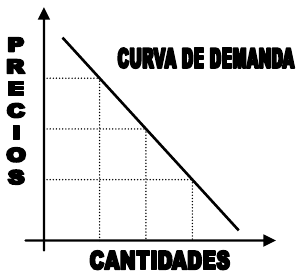
\includegraphics[width=0.31\linewidth]{figuras/fig_p060_26.png}
\end{center}

Abandonando la hipótesis de proporcionalidad o linealidad, las curvas de demanda tienen el aspecto mostrado. Ellas corresponden al llamado curva normal de demanda.


\begin{center}
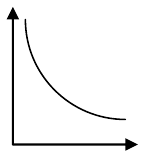
\includegraphics[width=0.15\linewidth]{figuras/fig_p060_27.png}
\end{center}

\begin{center}
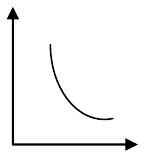
\includegraphics[width=0.15\linewidth]{figuras/fig_p060_28.png}
\end{center}

Algunos productos presentan curvas con aspectos muy diferentes a las vistas, en estos productos las demandas crecen a medida que aumenta el precio, en general son productos de lujo consumidas por parte de las clases de mayor poder adquisitivo, estas no prescinden de comprarlos aun cuando los precios suben, y hasta se da el caso de una baja del consumo cuando los precios bajan debido a que el prestigio de tales productos deriva precisamente de su alto precio. Otro aspecto de estas curvas es el de los llamados productos inferiores en los cuales una baja de precio determina una reducción de las cantidades demandadas debido a que los consumidores quedan con un sobrante de dinero para adquirir bienes de mejor calidad. A esta clase de curvas se les denomina curvas anómalas de la demanda.


\begin{center}

\includegraphics[width=0.88\linewidth]{figuras/fig_p060_29.png}
\end{center}

% ---- página 61 ----

\subsubsection*{LA OFERTA}
La oferta es la cantidad de un producto que los empresarios, o mejor, los vendedores están dispuestos a vender a precios determinados. El productor que fabrica un producto o el comerciante que lo vende, venderán o producirán mayores o menores cantidades según sea el precio vigente o esperado. Esto quiere decir que a mayor precio se ofrecerán mayores cantidades de un producto y menores cantidades cuando el precio es bajo.

La ley que podemos formular es que la oferta es función creciente del precio. Si elaboramos una tabla en la que se expresen las unidades de un producto que se ofrecerán a cada precio, podríamos representar la LEY DE OFERTA con el grafico siguiente:

{\raggedleft La curva creciente de la oferta relaciona\par}

{\raggedleft la cantidad ofrecida con el precio. Al\par}


\begin{center}
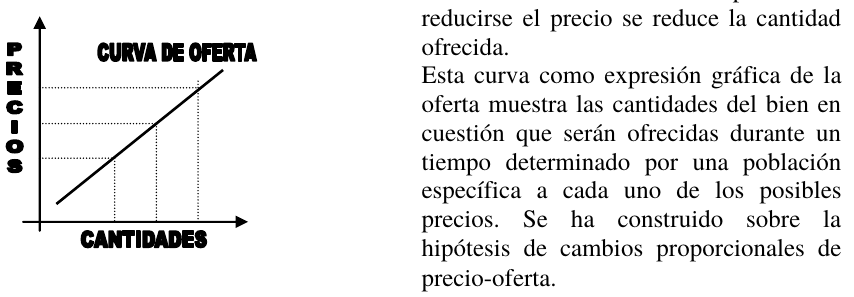
\includegraphics[width=0.87\linewidth]{figuras/fig_p061_30.png}
\end{center}

El precio que los vendedores están dispuestos a aceptar dependerá también del apuro que tengan por vender (caso de los productos perecederos), influencia el costo de conservar el bien (espacios, almacenes) y por los compromisos financieros.

Se advierte que la curva de oferta, como también la de demanda, son curvas estáticas, esto es, que ambas representa las cantidades que se ofrecen hoy a los distintos precios, y pueden representar la sumas de todas las curvas estáticas de ofertas del producto.

\subsubsection*{EL EQUILIBRIO DEL MERCADO}
Cuando ponemos en contacto a compradores y vendedores en el mercado, el precio arbitrario no logra que las cantidades ofrecidas y demandadas coincidan. Solo un precio es el aceptado, siempre y cuando no existan factores exógenos que predeterminen los mismos, este precio es llamado precio de equilibrio.

El precio de equilibrio es aquel para el que la cantidad demandada es igual a la ofrecida, y esta


\begin{center}
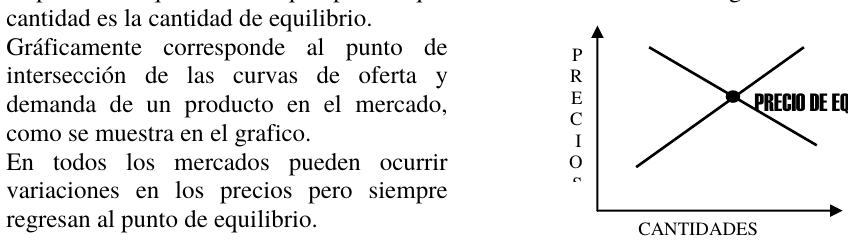
\includegraphics[width=0.87\linewidth]{figuras/fig_p061_31.png}
\end{center}

QUILIBRIO


% ---- página 62 ----

\section*{EL VALOR}
Entender el concepto de valor es necesaria para la formulación del precio, ya que el precio es la expresión concreta que se asigna a los bienes y servicios a través de la acción de la oferta y la demanda en los mercados, no obstante, a esta altura del conocimiento este concepto has sido objeto de apreciaciones muy diversas por parte de los economistas dando origen a diferentes teorías: Unas toman un criterio objetivo, como ocurre con el costo de producción, mientras otras toman como punto de partida un aspecto subjetivo (es decir una apreciación individual).

\subsubsection*{TEORÍA CLÁSICA DEL VALOR O TEORÍA OBJETIVA}
Establece que el valor de los bienes está determinado por su costo de producción, es decir por la suma de todos los gastos necesarios para fabricarlos.

Esta explicación del valor es criticada por ser unilateral, teniendo en cuenta solamente el punto de vista de la oferta y deja de lado la demanda que representa el deseo de adquirirlos por parte de los compradores. No explica porque algunos bienes adquieren más valor después de mucho tiempo de producidos como un mueble antiguo, un auto de colección, o los casos en que el bien cambia su valor según donde se vendan como el valor de la calefacción en los diferentes extremos de nuestro país, tampoco explica el valor alto de los bienes raros o únicos como las pinturas o esculturas, ni aquellos bienes que teniendo un mismo costo de producción tienen diferentes valores como el oro y el hierro.

\subsubsection*{TEORÍA SOCIALISTA DEL VALOR}
Establece que el valor está determinado por la cantidad de trabajo incorporado al bien, es decir que la medida del valor está dada exclusivamente por la cantidad de trabajo contenida en el bien producido.

A esta teoría se le pueden hacer las mismas críticas que a la anterior, no incluye tampoco los costos de los factores de producción, se deduce dentro de esta teoría que para un empresario que quisiera incrementar el valor de un bien seria ventajoso incorporar mayor trabajo, sin embargo una característica de la producción actual es la mecanización de la producción.

\subsubsection*{TEORÍA SUBJETIVA}
Da como fundamento del valor la utilidad del bien, es decir la importancia que el adquiriente del bien le asigna.

Las críticas a esta teoría es el de ser unilateral, se coloca del lado del comprador y no tiene en cuenta que el valor debe cubrir el costo de producción.

La noción de valor es, sin duda alguna, el eje alrededor del cual se edifica toda la economía, ya que si existe actividad económica de los hombres en torno a los bienes o servicios es porque se les atribuye valor, y los problemas económicos son ante todo problemas de valoración.

\section*{COSTOS}
Los costos también forman la base de los precios de venta de los productos, por lo que resulta necesaria una breve explicación del concepto y su incidencia en el precio.

En toda empresa productora se encuentran dos funciones la de producir y distribuir originando por lo tanto gastos de producción y distribución. Estas erogaciones se denominan costos. Es


% ---- página 63 ----

evidente la necesidad de obtener costos convenientes en las aludidas funciones, si obtengo costos reducidos en el área de producción pero son altos en el área de distribución el precio de venta puede no variar, lo mismo ocurriría de lo contrario por lo que se deben reducir ambos. A la actividad relacionada con el estudio de costos se la denomina Análisis de Costos, y es una de las funciones del área contable de toda organización.

El esquema siguiente indica los costos y los sectores que la generan:


\begin{center}
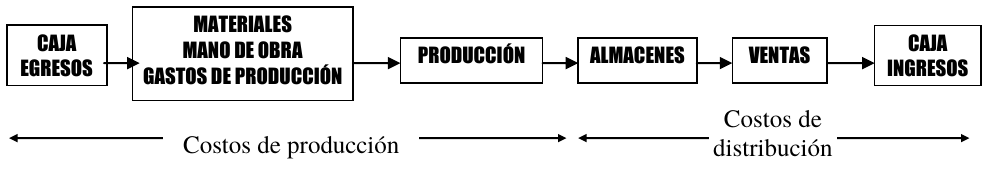
\includegraphics[width=1.00\linewidth]{figuras/fig_p063_32.png}
\end{center}

El costo de producción está integrado por todas las erogaciones que realiza la empresa para producir un bien, desde la transformación de los materiales hasta la obtención del producto y su colocación de los productos terminados en el almacén. Desde allí se producen los costos de distribución.

El proceso de la producción requiere la existencia del \textit{espacio }necesario para realizar las operaciones correspondientes, la disponibilidad de \textit{materiales}, y la \textit{mano de obra }que las transforme, la \textit{maquinaria }que amplía el esfuerzo humano, los \textit{medios }indispensables para el desarrollo, y la \textit{dirección }de los trabajos inherentes a la existencia propia de la explotación, aspectos que generan desembolsos que clasificados y considerados adecuadamente, facilitan la determinación de los costos.

Pertenecen a los costos de producción los materiales, mano de obra y gastos de producción. Se debe tener en cuenta que no siempre el volumen de producción obtenido con el mínimo costo es que proporciona el mayor beneficio.

\subsubsection*{CLASIFICACIÓN DE LOS COSTOS}
Según su clase o naturaleza:

1)  MATERIALES: Volumen físico de las materias primas que han de requerir los procesos productivos, precio de las materias primas.

2)  MANO DE OBRA: Cantidad de personal de utilización obligada, horas - hombre de producción, sistema de retribución de la mano de obra.

3)  GASTOS VARIOS: Gastos de producción fijos y variables.

Según la relación que tengan con la unidad de producto en:

1)  DIRECTOS: Madera y pintura de un mueble a fabricar.

2)  INDIRECTOS: Alquileres, seguros, luz.

Según el comportamiento de los costos con las variaciones del volumen producido 1)  VARIABLES: Materia prima, energía, transportes.

2)  FIJOS: Sereno, capataces, amortizaciones.

La clasificación moderna establece una mezcla de todas las anteriores .Por ejemplo: Costo de mano de obra indirecta como serenos, mantenimiento, tiempo improductivo, ayudantes generales.

El siguiente gráfico indica como se clasifican los costos:


% ---- página 64 ----

\begin{center}
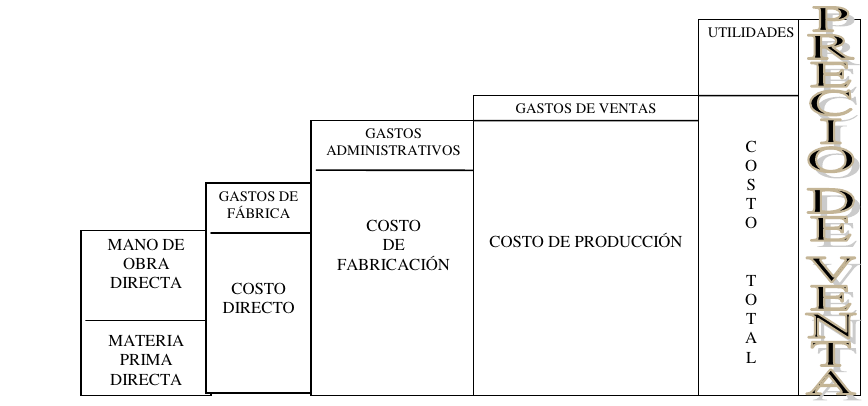
\includegraphics[width=0.89\linewidth]{figuras/fig_p064_33.png}
\end{center}

\subsubsection*{EJEMPLOS DE COSTOS EN LA ACTIVIDAD AERONÁUTICA}
BAJOS COSTOS DE MANTENIMIENTO Y ALTA CONFIABILIDAD Los bajos costos de mantenimiento y la alta confiabilidad de despacho son las claves para el éxito de una aerolínea.

En la competitiva industria de las aerolíneas, los bajos \textbf{Costos Directos de Operación }(CDO) son principales para la productividad de estas empresas. Los cinco elementos del CDO son: Costos de Propiedad, Costos de Tripulación y Auxiliares, Costos de Combustible, Costo de


\begin{center}
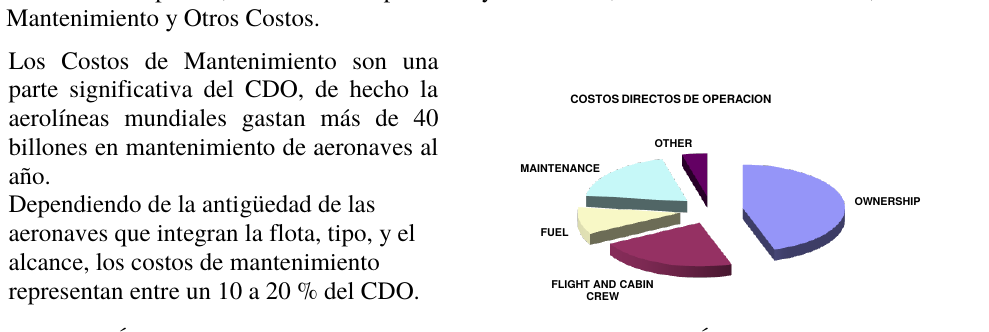
\includegraphics[width=1.00\linewidth]{figuras/fig_p064_34.png}
\end{center}

\subsubsection*{DEFINICIÓN DE LOS COSTOS DE MANTENIMIENTO AERONÁUTICO}
En la industria del transporte aéreo se describe los costos de mantenimiento como los gastos requeridos para restaurar o mantener los sistemas, componentes, y estructura de una aeronave a la condición de aeronavegabilidad. Estos costos incluyen gastos directos por mantenimiento de estructuras, motor y generales.

Los costos directos de mantenimiento de la estructura y motor, son los costos de mano de obra y materiales requeridos para reparar, modificar, restituir, inspeccionar, probar, y troubleshooting task durante las actividades del taller de mantenimiento.

Los costos generales de mantenimiento son costos laborales no asignados y gastos por supervisión del mantenimiento, entrenamiento y planificación, alquiler de equipos y elementos. En estos costos no se incluye los gastos por pruebas de equipos, herramientas y equipo de soporte de tierra.

Para ayudar a los operadores y fabricantes de aeronaves a entender los costos relativos de mantenimiento más característicos de las aeronaves y los factores que influencian estos costos,


% ---- página 65 ----

los costos totales de mantenimiento de un modelo específico de aeronaves pueden ser subdivididos de diferentes formas.

Un método consiste en dividir los costos de mantenimiento de acuerdo con los sistemas de la aeronave, como los define los capítulos de Air Transport Association (ATA).

La información de costos según los diferentes capítulos del ATA son usados para analizar los efectos de los cambios en el diseño y los costos de los proyectos de mantenimiento para aeronaves nuevas o serie de las anteriores.

Otra opción es dividir los costos directos de mantenimiento total de acuerdo a las actividades rutinarias y no rutinarias.

El mantenimiento rutinario comprende todas las tareas planeadas en un programa de mantenimiento de aerolínea. Un mantenimiento no rutinario incluye reparaciones no programadas, remociones y restauración de componentes. Los costos de material y trabajo en el mantenimiento no rutinario son la primordial causa del incremento del costo de mantenimiento en las aeronaves antiguas.

Los operadores y fabricantes se esfuerzan para reducir el mantenimiento no rutinario por sus efectos sobre la confiablidad y el tiempo de vuelo de las aeronaves.


\begin{center}
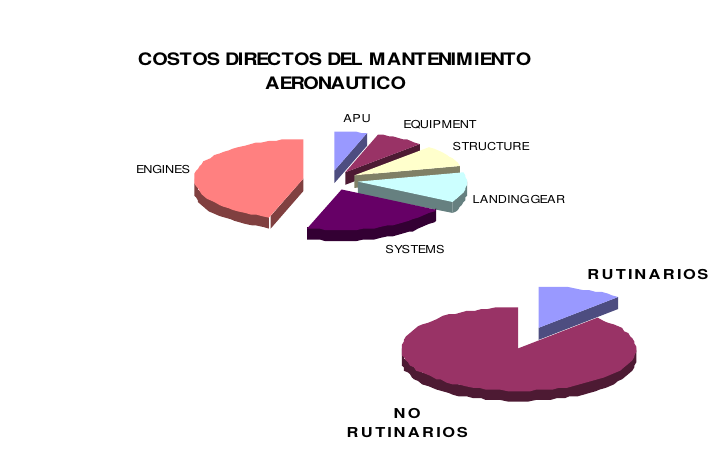
\includegraphics[width=0.74\linewidth]{figuras/fig_p065_35.png}
\end{center}

\subsubsection*{CUESTIONARIO 5}
1. ¿Qué es la Economía?

2. Definir necesidades humanas.

3. Dar ejemplos de cada tipo de necesidades humanas.

4. ¿A qué se llama Microeconomía? Dar ejemplos.

5. ¿A qué se llama Macroeconomía? Dar ejemplos.

6. ¿Cuál es la suposición fundamental en los modelos económicos?

7. ¿Cuándo se considera que una teoría es válida?

8. ¿Si la economía es una disciplina científica por qué existen tantas discrepancias entre los economistas?

9. ¿Cuál es la definición económica de Bien?

10. ¿A qué se llama escasez? Dar un ejemplo que ilustre sobre el concepto de escasez.


% ---- página 66 ----

11. Definir los factores productivos.

12. Dar ejemplos de recursos naturales renovables y no renovables.

13. Dar ejemplos de capital humano.

14. ¿Qué son los Mercados? Mencionar cuatro ejemplos de Mercados.

15. ¿Qué diferencia existe entre mercados libres o intervenidos?

16. ¿Qué son los mercados de competencia perfecta e imperfecta?

17. ¿Cuáles son las hipótesis de los mercados perfectos?

18. ¿Qué es la demanda?

19. ¿Qué hipótesis se adoptan para analizar la demanda?

20. ¿Qué establece la Ley de Demanda? ¿Cuáles son las variables relacionadas?

21. ¿Cómo se explica la variación de la demanda?

22. ¿Qué es la oferta?

23. ¿Cuál es la hipótesis adoptada en la oferta?

24. ¿Qué variables se relacionan?

25. ¿Cómo se explica esta variación?

26. ¿Cómo surge el precio de equilibrio?

27. ¿Cuál es la representación gráfica de la demanda de un producto de lujo?


% ---- página 67 ----

\subsubsection*{CONTENIDOS DEL NÚCLEO TEMÁTICO QUINTO}
Las relaciones jurídicas: Contratos. Contratos comerciales. Contratos laborales: Características, clases, nuevas formas de contratación, leyes laborales. Ley de riesgos del trabajo. Asignaciones familiares. Obras sociales. Propiedad intelectual. Propiedad Industrial: Marcas y patentes. Derecho del autor. Principios de Legislación Aeronáutica.

\section*{RELACIONES JURÍDICAS}
\subsubsection*{INTRODUCCIÓN}
Desde que nos levantamos por la mañana para realizar nuestras actividades diarias hasta que nos acostamos estamos en contacto con el orden jurídico también llamado derecho. El derecho de un modo u otro está en todas las relaciones sociales. Las personas humanas somos, por esencia, sociales. Nos relacionamos en la medida en que somos y somos en la medida en que nos relacionamos. En la vida en sociedad cada persona tiene sus propios intereses y sus particulares necesidades, problemas, deseos y también las de otras personas por la que siente simpatía o afecto como los familiares o amigos. Básicamente la función del derecho consiste en hacer posible la vida de las personas en sociedad. Para ello, el derecho toma en cuenta diferentes circunstancias, tales como la importancia de que todas las personas tengan un ámbito de privacidad en el cual pensar, hacer, y sentir como quieran; los valores y los fines de la sociedad como la justicia, el bienestar general, la paz, la cooperación, la solidaridad, la tolerancia; las necesidad de compatibilizar los intereses individuales con los de la sociedad, y las conductas discriminatorias, egoístas, indiferentes e individualistas de muchas personas en relación con otras.

Como toda clasificación propia de una persona, la que sigue es arbitraria, designando a las Relaciones con minúscula o mayúscula según que importen o no para el derecho:


\begin{center}
\small
\begin{tabular}{|p{\dimexpr0.171\linewidth-2\tabcolsep\relax}|p{\dimexpr0.401\linewidth-2\tabcolsep\relax}|p{\dimexpr0.428\linewidth-2\tabcolsep\relax}|}
\hline
 & Relaciones & RELACIONES \\ \hline
 & Vinculaciones humanas SIN trascendencia jurídica & Vinculaciones humanas CON trascendencia jurídica \\ \hline
EJEMPLOS & La amistad & El matrimonio los contratos \\ \hline
\end{tabular}
\end{center}

Para cumplir una función tan compleja de regular las relaciones jurídicas, existen las normas, que son reglas que regulan las conductas de las personas y también a los diferentes grupos que integran la sociedad. Estas normas pueden ser escritas o no. Los estados tienen la responsabilidad de establecer los mecanismos de regulación y control de las actividades que realiza el hombre. Esta regulación de las actividades del hombre se realiza mediante la sanción de distintas normas que ordenan y organizan la vida de las personas para poder vivir en sociedad. Las leyes son un tipo de normas escritas dictadas por el Congreso y de carácter obligatorio que rige una determinada cuestión considerada importante para la vida social y el desarrollo de un país. Los contratos constituyen otro tipo de norma escrita que contribuyen a reglamentar la interacción de las personas en la sociedad. Las costumbres son otra importante clase de normas a la que acude el derecho para organizar la convivencia social. Estas son las conductas realizadas por las personas a lo largo del tiempo de manera generalizada. Las costumbres no están escritas


% ---- página 68 ----

en ninguna parte, ni tienen su origen en ninguna autoridad, ni en el acuerdo de varias personas. Las sentencias de los jueces son otro ejemplo de normas de las que se vale el derecho. Pero a diferencia de las anteriores, una sentencia regula las conductas de las personas que han intervenido en un caso judicial en el que la sentencia es dictada y es obligatoria. Finalmente la norma básica del orden jurídico de un país es su Constitución. Esta es la norma fundamental que contiene el programa por el cual se organiza un país.

La pregunta de que es el derecho o el orden jurídico no es fácil de contestar. Existen diferentes posturas que han establecido lo que se entiende por derecho u orden jurídico. Algunos conceptos son nuevos y otros antiguos. Los conceptos antiguos no son reaplazados por los conceptos nuevos, ni se corrigen entre ellas. Las posturas son diferentes entre sí pero conviven con nuevos elementos que la tornan más actuales. Cada postura brinda un concepto del derecho pero no establece que es el derecho, cada individuo deberá identificarse con la postura que más se acerca a lo que entiende por derecho porque no resulta posible establecer una única definición.

\subsubsection*{PERSONAS FÍSICAS Y PERSONAS JURÍDICAS}
En el derecho el concepto de persona es más amplio que el concepto cotidiano que tenemos de la palabra. Para el derecho las personas pueden ser el hombre y ciertas organizaciones en cuanto tienen la condición de adquirir derechos y obligaciones. Por esto en el derecho se habla de persona física y de persona jurídica. La persona física es la persona individual, humana. La persona jurídica es la persona colectiva, social como algunas organizaciones.

\section*{CONTRATOS}
Los contratos son convenciones que celebran las personas entre sí para regular un tema en particular que los vincula, determinando los derechos de cada parte, sus deberes y las acciones en caso de incumplimiento de una parte. De esta forma, el contrato es un acuerdo de voluntades destinado a reglar los derechos.

La voz contrato proviene de contractus, expresión latina que significa unir, estrechar, o contraer. El Código Civil Argentino define al contrato de la siguiente forma:

\textbf{\textit{Habrá contrato cuando dos o más personas se ponen de acuerdo sobre una declaración de}}

\subsection*{voluntad común destinada a reglar sus derechos.}
\subsubsection*{ACTOS JURÍDICOS}
Del código civil: Son actos jurídicos los actos voluntarios lícitos, que tengan por fin inmediato, establecer entre las personas relaciones jurídicas, crear, modificar, transferir, conservar o aniquilar derechos. La nota más distintiva del acto jurídico de los contratos es su fin jurídico: nacimiento, modificación, o extinción de una relación jurídica. El contrato presenta las siguientes notas distintivas:

\begin{itemize}
  \item \textit{Puede ser bilateral (suministro), unilateral (testamento) o plurilateral (creación de} \textit{sociedades).}
  \item \textit{Es entre vivos, por no depender del fallecimiento de aquellos de cuya voluntad emanan.}
  \item \textit{Es patrimonial.}
  \item \textit{Es causado.}
\end{itemize}
El Contrato puede tener también por objeto crear un sujeto jurídico: la sociedad civil, la asociación.


% ---- página 69 ----

\subsubsection*{LA IMPORTANCIA DEL CONTRATO}
El contrato es el principal instrumento de que se valen los hombres para sus relaciones jurídicas, es decir, es la principal fuente de las obligaciones y derechos. El hombre vive contratando o cumpliendo contratos, desde operaciones de gran envergadura, hasta contratos cotidianos que el hombre realiza muchas veces sin darse cuenta (de trabajo, de transporte, etc.) Es claro que el contrato adquiere su máxima importancia en un régimen de economía capitalista liberal. Desde el punto de vista ético, la importancia se aprecia desde un doble ángulo: Por una parte, hay una cuestión moral envuelta en el deber de hacer honor a la palabra empeñada; por la otra, los contratos deber ser un instrumento de la realización del bien común.

\subsubsection*{REGLAS SOBRE LOS CONTRATOS}
1.- Los contratos son obligatorios. Las obligaciones que establecen tienen fuerza de ley para los contratantes.

2.- La obligatoriedad deriva de la voluntad de las partes, reconocida y amparada por la ley. 3.- La obligatoriedad se extiende a todas las consecuencias del contrato, aún no expresadas siempre que deriven de la naturaleza del contrato conforme a la buena fe, al uso o a la ley. 4.- Como consecuencia de la obligatoriedad, la validez y el cumplimiento del contrato no pueden quedar al arbitrio de uno solo de los contratantes.

5.- Solo las partes del contrato de común acuerdo y siempre que no perjudique a terceros, pueden modificar o anular el contenido de un contrato.

6.- Los contratos solo producen efecto entre las partes que los otorgan y sus herederos (a menos que las obligaciones sean intransmisibles).

\subsubsection*{MODOS DE EXTINCIÓN DE LOS CONTRATOS}
1. Por cumplimiento del plazo convenido en el mismo.

2. Por revocación por una de las partes fundada en causa legal.

3. Por fallecimiento de una de las partes, siempre que las obligaciones sean intrasmisibles.

\section*{CONTRATOS COMERCIALES}
En la vida diaria celebramos contratos comerciales sin percibir que estamos contrayendo derechos y obligaciones, al subir a un medio de transporte como un colectivo celebramos un contrato comercial de transporte por medio del cual, mediante el pago que realizamos contratamos el transporte en la forma y tiempo programado por el transportador, el boleto es el comprobante otorgado por la compañía que prueba la realización del contrato.

El contrato comercial es un acuerdo de voluntades destinado a reglar los derechos patrimoniales. Las actividades comerciales se encuentran descriptas en el Código de Comercio. Algunos ejemplos de contratos comerciales son:

1) CONTRATO DE SUMINISTRO: Las condiciones del contrato vienen establecidas por una sola de las partes. El contenido del contrato se establece unilateralmente, y la otra parte no puede modificarlo (teléfono, agua, gas, luz).

2) CONTRATO DE LEASING: Intervienen dos o más partes en el alquiler de un bien mueble o inmueble con opción a compra.


% ---- página 70 ----

3) PRÉSTAMO BANCARIO:

El préstamo bancario es el contrato por el cual un banco entrega a su cliente una suma determinada de dinero, obligándose el cliente a restituirla en la misma especie y cantidad en el plazo convenido pagando los intereses pactados.

4) CONTRATO DE TRANSFERENCIA ONEROSA DE MARCA COMERCIAL:

{\raggedleft Permiso para\par}

utilizar o autorizar a terceros a utilizar la marca de conformidad con términos convenidos.

5) CONTRATO DE DISTRIBUCIÓN:

Se celebran cuando una empresa concede a una distribuidora la exclusividad para comercializar sus productos en una determinada zona.

6) CONTRATO DE EDICIÓN:

Se celebra entre dos partes cuando un autor de una obra otorga a un editor su obra en exclusividad, para que se imprima, difunda y venda.

7) CONTRATO DE AGENCIA O REPRESENTACIÓN:

{\raggedleft Se celebra entre una empresa que autoriza\par}

a un agente para que en la una zona, ciudad, barrio etc. realice determinadas operaciones comerciales en nombre o utilizando el nombre de la empresa.

8) CONTRATO DE MANDATO:

Es el caso en el cual el mandante solicita al mandatario y éste acepta la realización de una determinada tarea.

9) CONTRATO DE COMODATO: El comodante entrega al comodatario y éste recibe en préstamo de uso gratuito un inmueble.

10) CONTRATO SOCIAL: Es el contrato por el cual se establece la creación de una sociedad comercial. La creación de una persona jurídica.

Otras clases de contratos comerciales son el Contrato de Concesión, Arrendamiento Rural, Suministro, Franquicia, Locación de Cochera, Locación de guardería Náutica.


% ---- página 71 ----

\begin{center}
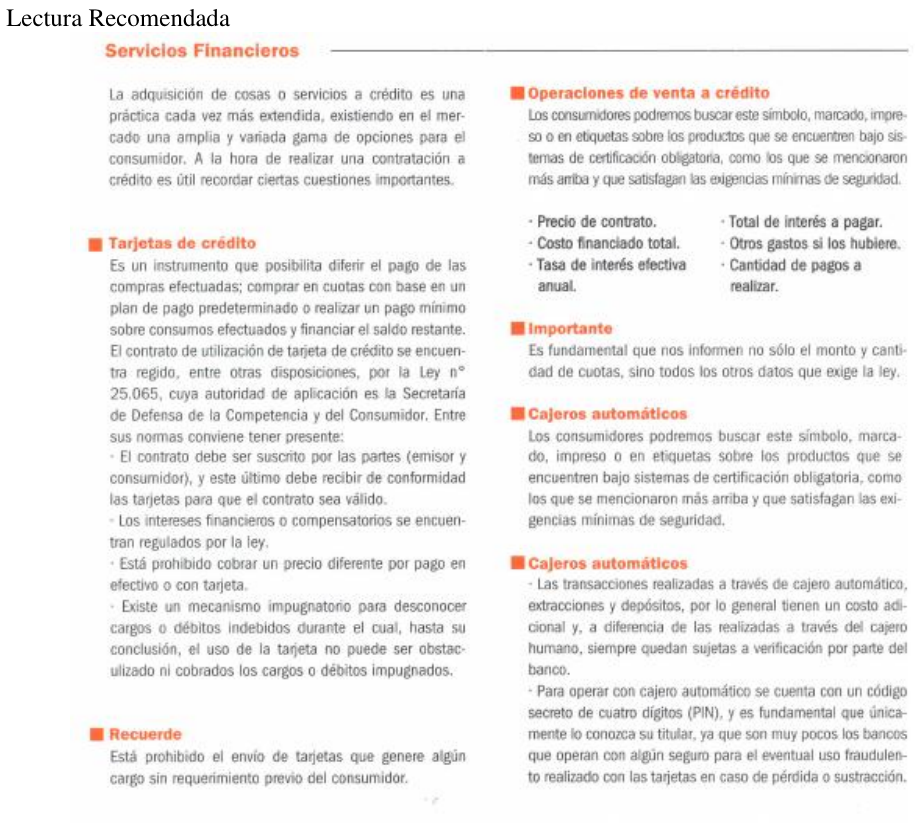
\includegraphics[width=0.94\linewidth]{figuras/fig_p071_36.png}
\end{center}

% ---- página 72 ----

\begin{center}
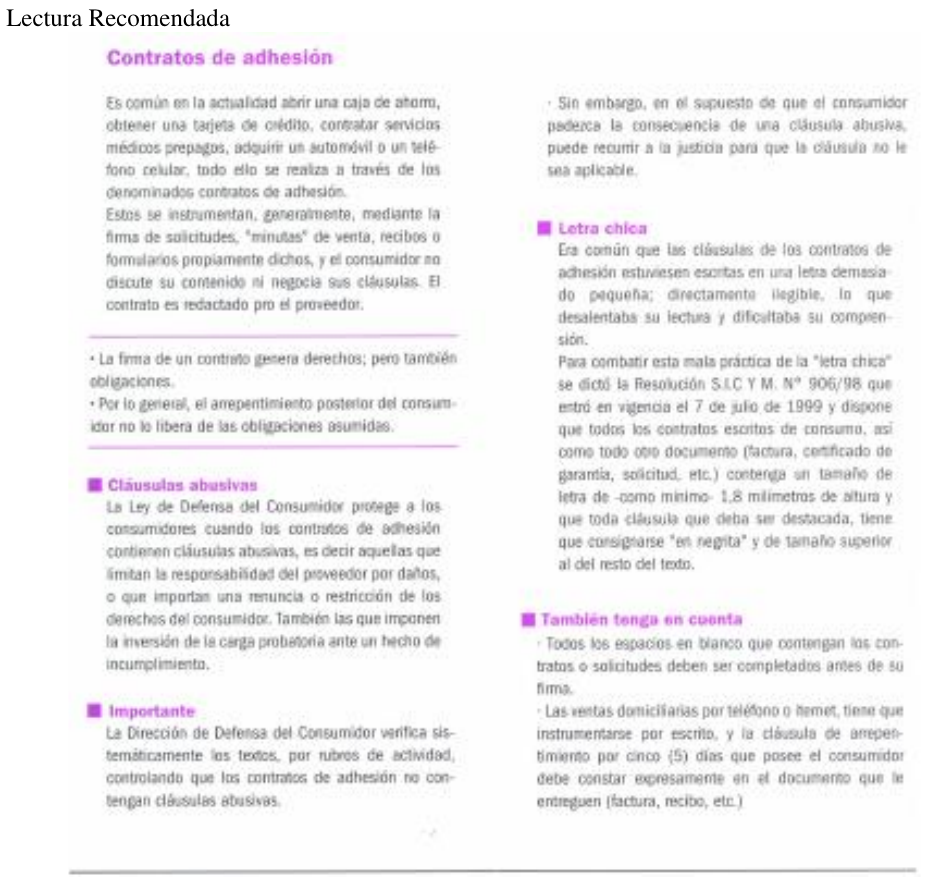
\includegraphics[width=0.95\linewidth]{figuras/fig_p072_37.png}
\end{center}

\section*{CONTRATOS LABORALES}
El contrato es un acuerdo de voluntades destinado a reglar los derechos y obligaciones laborales. El Derecho del Trabajo regula relaciones jurídicas de acuerdo a diversos planos que se dan en la realidad laboral. Regula la relación Trabajador - Empleador, estos son los protagonistas genéricos del derecho laboral, esto es el Derecho Individual del Trabajo que se apoya en el contrato. En este plano se regulan las relaciones obrero-patronales. Pero el Derecho del Trabajo atiende también a un Fenómeno Colectivo, es decir, un conjunto de cosas que pasan, relaciones de grupo, necesidades y angustias de los trabajadores, que ante las desventajas en las que se encuentran individualmente frente a su empleador (trabajadores y empleadores serán los sujetos del Derecho del Trabajo), los trabajadores se agrupan tras un interés colectivo enfrentado al de la empresa: adoptan la forma de organización sindical. Estas serán las que negociarán con los empleadores, y no el trabajador individual. El Fenómeno Colectivo tiene tres etapas Asociación, Negociación y Conflicto. Para evitar llegar a la etapa del conflicto se busca un acuerdo, este acuerdo constituye los Convenios Colectivos de Trabajo.


% ---- página 73 ----

\subsubsection*{CARACTERÍSTICAS DE UN CONTRATO DE TRABAJO}
¿Entre quienes se acuerdan estos contratos?

Trabajador: Es toda persona física que se obliga a realizar actos, ejecutar obras, o prestar un servicio bajo la dependencia de otra persona mediante el pago de una remuneración.

Empleador: Es toda persona física o jurídica que se obliga a pagar una remuneración a cambio de actos, obras o servicios realizados por el trabajador.

¿Quién puede firmar un Contrato laboral?

\begin{itemize}
  \item Las personas mayores de 18 años.
  \item Los mayores de 16 y menores de 18 años legalmente emancipados.(cuando contraen matrimonio o por autorización de un juez)
  \item Las personas mayores de 16 y menores de 18 si viven de forma independiente con el consentimiento expreso o tácito de sus padres o tutores o si tienen autorización de los padres o de quien los tenga a su cargo.
  \item Los extranjeros de acuerdo con la legislación que les sea aplicable.
\end{itemize}
¿Cómo se extingue un contrato laboral?

\begin{itemize}
  \item Por cumplimiento del plazo convenido en el mismo.
  \item Por rescisión de cualquiera de las partes fundada en el incumplimiento de la otra parte.
  \item Por el fallecimiento del empleado.
\end{itemize}
¿Cómo puede formalizarse un Contrato?

El Contrato de trabajo puede formalizarse por escrito o de palabra.

¿Cuándo es obligatorio realizarlo por escrito?

\begin{itemize}
  \item Deberá celebrarse por escrito cuando así lo exija una disposición legal.
  \item Igualmente constarán por escrito los contratos por tiempo determinado, cuya duración sea superior a cuatro semanas.
  \item Cualquiera de las partes podrá exigir que el contrato se celebre por escrito, incluso durante el transcurso de la relación laboral.
\end{itemize}
Obligaciones del empleador

\begin{itemize}
  \item \textbf{Con el trabajador}
\end{itemize}
Cuando la relación laboral sea de duración superior a cuatro semanas, el empresario deberá informar por escrito al trabajador sobre los elementos esenciales del contrato y principales condiciones de ejecución de la prestación laboral, siempre que tales elementos y condiciones no figuren en el contrato de trabajo formalizado por escrito.

\begin{itemize}
  \item \textbf{Con los representantes legales de los trabajadores}
\end{itemize}

% ---- página 74 ----

También deberá entregar a los representantes legales de los trabajadores, una copia básica de los contratos formalizados por escrito (con excepción de los contratos de relaciones especiales de alta dirección, para los que es suficiente la notificación), así como las prórrogas de dichos contratos y las denuncias de los mismos, teniendo para ello el mismo plazo de 10 días. La copia básica contendrá todos los datos del contrato a excepción del número del Documento Nacional de Identidad, domicilio, estado civil y cualquier otro dato que pudiera afectar a la identidad personal del interesado.

Duración de un contrato de trabajo

\begin{itemize}
  \item En principio todos los contratos de trabajo son por tiempo indeterminado salvo que se establezca expresamente por escrito en el contrato el plazo de su duración.
  \item Las normas que regulan cada tipo de contrato temporal establecen cual es la duración mínima y máxima del contrato.
\end{itemize}
Período de prueba en un contrato de trabajo (Ley de contrato de Trabajo 20744)

\begin{itemize}
  \item Su establecimiento es optativo y de acordarlo, se deberá reflejar por escrito en el contrato.
  \item Su duración máxima se establecerá en los Convenios Colectivos, y en su defecto la duración no podrá exceder de tres meses.
  \item Durante el período de prueba, el trabajador tendrá los mismos derechos y obligaciones correspondientes al puesto de trabajo que desempeñe como si fuera de plantilla.
  \item Durante este período se podrá rescindir la relación laboral por voluntad de cualquiera de las partes, con preaviso sin alegar causa alguna y sin derecho a indemnización.
  \item El período de prueba se computa a efectos de antigüedad.
  \item La situación de incapacidad temporal que afecte al trabajador durante el período de prueba interrumpirá el cómputo del mismo, siempre que se produzca acuerdo entre ambas partes.
  \item En las Empresas con menos de 25 trabajadores, el período de prueba no podrá exceder de tres meses para los trabajadores que no sean Técnicos Titulados.
  \item No se podrá establecer período de prueba cuando el trabajador haya ya desempeñado las mismas funciones con anterioridad en la Empresa, bajo cualquier modalidad de contratación.
\end{itemize}
Qué derechos y/o obligaciones conlleva la firma de un contrato

\begin{itemize}
  \item Un contrato de trabajo supone unos derechos para el trabajador, que se convierten en obligaciones para el empresario. Al mismo tiempo, las obligaciones que contrae el trabajador se convierten en derechos de su empresario.
\end{itemize}
Cuáles son los derechos del trabajador

\begin{itemize}
  \item A la ocupación efectiva durante la jornada de trabajo.
  \item A la promoción y formación en el trabajo
  \item A no ser discriminados para acceder a un puesto de trabajo.
  \item A la integridad física y a la intimidad.
  \item A percibir puntualmente la remuneración pactada.
  \item Los demás que se establezcan en el contrato de trabajo.
\end{itemize}

% ---- página 75 ----

¿Cuáles son los deberes del trabajador?

\begin{itemize}
  \item Cumplir las obligaciones concretas del puesto de trabajo conforme a los principios de la buena fe y diligencia.
  \item Cumplir las medidas de seguridad e higiene que se adopten.
  \item Cumplir las órdenes e instrucciones del empresario en el ejercicio de su función directiva.
  \item No realizar la misma actividad que la empresa en competencia con ella (fidelidad).
  \item Contribuir a mejorar la productividad.
  \item Los demás que se establezcan en el contrato de trabajo.
\end{itemize}
\subsection*{MODELO DE CONTRATO POR SERVICIOS PROFESIONALES}
En la ciudad de Buenos Aires a los \_\_\_\_\_\_ días del mes de \_\_\_\_\_, se celebra el presente contrato por locación de servicios profesionales entre \_\_\_\_\_\_\_\_\_\_\_\_\_\_\_\_\_\_\_\_\_\_\_\_\_\_\_\_\_\_\_\_\_\_\_\_\_\_\_, por una parte y por la otra los hace el Sr.\_\_\_\_\_\_\_\_\_\_\_\_\_\_\_\_\_\_\_\_\_\_\_\_\_\_\_\_\_\_\_\_\_\_\_\_\_\_\_\_\_\_\_, domiciliado en \_\_\_\_\_\_\_\_\_\_\_\_\_\_\_\_\_\_\_\_\_\_\_\_\_\_\_\_\_\_\_\_, de \_\_\_\_\_\_\_\_\_\_\_\_\_\_\_\_\_\_\_\_\_\_\_\_en adelante identificado como “el contratado”, con documento de identidad número \_\_\_\_\_\_\_\_\_\_\_\_\_\_, quien declara ser de nacionalidad \_\_\_\_\_\_\_\_\_\_\_\_\_\_\_\_, de estado civil \_\_\_\_\_\_\_\_\_\_\_\_\_\_\_\_, de profesión \_\_\_\_\_\_\_\_\_\_\_\_\_\_\_\_\_\_\_\_\_\_.

El presente contrato de locación de servicios profesionales se convienen encuadrarlo específicamente en lo determinado por el Capítulo VIII-ART 1623 siguientes y concordantes del Código Civil Argentino y en un todo de acuerdo a los términos y condiciones particulares que seguidamente se enuncian:

\subsubsection*{1. OBJETO Y FUNCIONES}
El contratado prestara sus servicios de \_\_\_\_\_\_\_\_\_\_\_\_\_\_\_\_\_\_\_\_\_\_\_\_\_\_\_\_\_ en el horario de \_\_\_\_\_\_\_\_ a \_\_\_\_\_\_\_\_, de \_\_\_\_\_\_\_\_\_\_ a \_\_\_\_\_\_\_\_\_\_\_, en \_\_\_\_\_\_\_\_\_\_\_\_\_\_\_\_\_\_\_\_\_\_\_\_\_\_, bajo las órdenes de \_\_\_\_\_\_\_\_\_\_\_\_\_\_\_\_\_\_\_\_\_\_\_\_\_, realizando las tareas de \_\_\_\_\_\_\_\_\_\_\_\_\_\_\_\_\_\_\_\_\_.

\subsubsection*{2. DURACIÓN DEL CONTRATO}
El plazo de ejecución del presente contrato es de \_\_\_\_ meses, a partir del \_\_\_\_\_\_\_\_\_\_, finalizando el \_\_\_\_\_\_\_\_\_\_\_\_\_\_\_\_\_\_.

Queda establecido que este contrato no importa una expectativa o derecho a prorroga a beneficio del contratado, pudiendo ser prorrogado o renovado únicamente de común acuerdo entre las partes mediante suscripción de un nuevo contrato. La continuación en la prestación de los servicios una vez operado el vencimiento del contrato no importa en modo alguno la tacita reconducción del mismo.

\subsubsection*{3. RETRIBUCIÓN}
El honorario total por todo concepto se ha convenido en \$\_\_\_\_\_\_\_\_\_\_\_, pagaderos en libramientos mensuales. El primero a efectuarse el quinto día hábil del mes subsiguiente a la iniciación del contrato, y el resto de los meses dentro de los primeros cinco días hábiles del mes siguiente a la prestación del servicio.

\subsubsection*{4. VIÁTICOS}
En caso de corresponder viáticos por traslados debido a la actividad laboral, los mismos serán pagados en su totalidad por la organización contratante.

\subsubsection*{5. APORTES JUBILATORIOS Y PRESTACIONES MÉDICAS}
El contratado manifiesta estar inscripto en la Caja de Previsión de Argentina, en la cual efectúa y continuara efectuando sus aportes provisionales.

A tal fin declara que su desempeño profesional es independiente y autónomo, comprendido en las disposiciones de la ley Nro. 18038, cuyo puntual y estricto cumplimiento correrá por cuenta exclusiva, como así también toda otra obligación derivada de la legislación impositiva, provisional, de seguridad y asistencia aplicables en la República Argentina.

\subsubsection*{7. RESCISIÓN}
Cada una de las partes podrá, en todo momento, rescindir el presente contrato, notificando por escrito a la otra parte con 15 días de anticipación.


% ---- página 76 ----

\subsubsection*{8. DERECHO DE PROPIEDAD}
Los derechos de propiedad de autor y de reproducción, así como cualquier otro derecho intelectual de cualquier naturaleza que sea, sobre cualquier informe, trabajo, o estudio u otra producida como consecuencia de este contrato, pertenecerá exclusivamente al contratante.

\_\_\_\_\_\_\_\_\_\_\_\_\_\_\_\_\_\_\_\_\_\_\_\_\_\_                                    \_\_\_\_\_\_\_\_\_\_\_\_\_\_\_\_\_\_\_\_\_\_\_\_\_\_\_\_\_

Contratante o Representante Legal                                                                                                                       Contratado

Firma y Aclaración                                                                                                                              Firma y Aclaración

\subsubsection*{RÉGIMEN DE CONTRATO DE TRABAJO LEY 20744}
EXTRACCIÓN DE ALGUNOS DE LOS PRINCIPALES ARTÍCULOS DEL RÉGIMEN DE CONTRATO DE TRABAJO (Reformada por la ley 21297 actualizada y concordada con la ley nacional de empleo 24013 y la ley de accidentes de trabajo)

\textbf{Artículo 115}°: El trabajo no se presupone gratuito.

\textbf{Artículo 21}°: Habrá contrato de trabajo, cualquiera sea su forma o denominación, siempre que una persona física se obligue a realizar actos, ejecutar obras, o prestar servicios a favor de la otra y bajo la dependencia de esta, durante un periodo determinado o indeterminado de tiempo, mediante el pago de una remuneración, las cláusulas, en cuanto a la forma y condiciones de prestación, quedan sometidas a las disposiciones de orden público, los estatutos, las convenciones colectivas, usos y costumbres.

\textbf{Artículo 4}°: Constituye trabajo, a los fines de esta ley, toda actividad licita que se preste a favor de quien tiene la facultad de dirigirla, mediante una remuneración .El contrato de trabajo tiene como principal objeto la actividad productiva y creadora del hombre en sí.

\textbf{Artículo 7}°: Las partes en ningún caso, pueden pactar condiciones menos favorables para el trabajador que las dispuestas en las normas legales, convenciones colectivas de trabajo, o que resulten contrarias a las mismas.

\textbf{Artículo 12}°: Será nula y sin valor toda convención de partes que suprima o reduzca los derechos previstos en esta ley, los estatutos profesionales o las convenciones colectivas, ya sea el tiempo de su celebración o de su ejecución, o del ejercicio de derechos provenientes de su extinción.

\textbf{Artículo 17}°: Por esta ley se prohíbe cualquier tipo de discriminación entre los trabajadores por motivos de sexo, raza, nacionalidad, religiosos, políticos, gremiales o de edad.

\textbf{Artículo 23}°: El hecho de la prestación de servicios hace presumir la existencia de un contrato de trabajo, salvo que por las circunstancias, las relaciones o causas que lo motiven se demuestre lo contrario.

\textbf{Artículo 38}°: No podrán ser objeto del contrato de trabajo las prestaciones de servicios ilícitos o prohibidos.

\textbf{Artículo 70}°: Los sistemas de controles personales del trabajador destinados a la protección de los bienes del empleador deberán siempre salvaguardar la dignidad del trabajador y deberán practicarse con discreción, los controles al personal femenino deberá estar reservados exclusivamente a personas de su miso sexo.

\textbf{Artículo 75}°: El empleador debe hacer observar las pausas y limitaciones a la duración del trabajo establecidas en esta ley y de las normas reglamentarias, y adoptar las medidas que según el tipo de trabajo, la experiencia y la técnica sean necesarias para tutelar la integridad psicofísica y la dignidad de los trabajadores.


% ---- página 77 ----

\textbf{Artículo 82}: Las invenciones o descubrimientos personales del trabajador son propiedad de este, aun cuando se haya valido de instrumentos que no le pertenecen. Las invenciones o descubrimientos que se deriven de los procedimientos industriales, métodos o instalaciones del establecimiento o de experimentaciones, investigaciones, mejoras o perfeccionamientos de los ya empleados, son de propiedad del empleador habiendo sido el empleado contratado para tal fin. \textbf{Artículo 85}: El trabajador debe observar todos aquellos deberes de fidelidad que deriven de la índole de las tareas que tenga asignadas, guardando reserva o secreto de las informaciones a que tenga acceso y que exijan tal comportamiento de su parte.

\textbf{Artículo 95}: En los contratos a plazo fijo, el despido injustificado dispuesto antes del vencimiento del plazo, dará derecho al trabajador, además de las indemnizaciones que correspondan por extinción del contrato en tales condiciones, a los daños y perjuicios provenientes del derecho común.

\textbf{Artículo 119}: Por ninguna causa podrán abonarse salarios inferiores a los que se fijen de conformidad al presente capitulo, salvo los que resulten de reducciones para aprendices o menores o para trabajadores de capacidad disminuida o de jornadas de trabajos reducidas. \textbf{Artículo 135}: Se podrá deducir o retener de la remuneración del empleado en el caso en que el trabajador hubiera causado daños graves e intencionales a los talleres, instrumentos o materiales de trabajo. El empleador deberá consignar judicialmente de la remuneración.

\textbf{Artículo 138}: Todo pago en concepto de salario u otra forma deberá instrumentarse mediante recibo firmado por el trabajador.

\textbf{Artículo 150}: Licencia ordinaria.

El trabajador gozará de un período mínimo y continuado de descanso anual remunerado por los siguientes plazos:

a) De catorce (14) días corridos cuando la antigüedad en el empleo no exceda de cinco (5) años. b) De veintiún (21) días corridos cuando siendo la antigüedad mayor de cinco (5) años no exceda de diez (10).

c) De veintiocho (28) días corridos cuando la antigüedad siendo mayor de diez (10) años no exceda de veinte (20).

d) De treinta y cinco (35) días corridos cuando la antigüedad exceda de veinte (20) años. Para determinar la extensión de las vacaciones atendiendo a la antigüedad en el empleo, se computará como tal aquélla que tendría el trabajador al 31 de diciembre del año que correspondan las mismas.

\textbf{Artículo }151: Requisitos para su goce.

Comienzo de la licencia. El trabajador, para tener derecho cada año al beneficio establecido en el artículo 150 de esta ley, deberá haber prestado servicios durante la mitad, como mínimo, de los días hábiles comprendidos en el año calendario o aniversario respectivo. A este efecto se computarán como hábiles los días feriados en que el trabajador debiera normalmente prestar servicios. La licencia comenzará en día lunes o el siguiente hábil si aquél fuese feriado. Tratándose de trabajadores que presten servicios en días inhábiles, las vacaciones deberán comenzar al día siguiente a aquél en que el trabajador gozare del descanso semanal o el subsiguiente hábil si aquél fuese feriado. Para gozar de este beneficio no se requerirá antigüedad mínima en el empleo.

\textbf{Artículo 15}: Tiempo trabajado. Su cómputo.

Se computarán como trabajados, los días en que el trabajador no preste servicios por gozar de una licencia legal o convencional, o por estar afectado por una enfermedad inculpable o por infortunio en el trabajo, o por otras causas no imputables al mismo.

\textbf{Artículo 153}: Falta de tiempo mínimo. Licencia proporcional.


% ---- página 78 ----

Cuando el trabajador no llegase a totalizar el tiempo mínimo de trabajo previsto en el artículo 151 de esta ley, gozará de un período de descanso anual, en proporción de un (1) día de descanso por cada veinte (20) días de trabajo efectivo, computable de acuerdo al artículo anterior. \textbf{Artículo 154}: Época de otorgamiento. Comunicación.

El empleador deberá conceder el goce de vacaciones de cada año dentro del período comprendido entre el 1. De octubre y el 30 de abril del año siguiente. La fecha de iniciación de las vacaciones deberá ser comunicada por escrito, con una anticipación no menor de cuarenta y cinco (45) días al trabajador, ello sin perjuicio de que las convenciones colectivas puedan instituir sistemas distintos acordes con las modalidades de cada actividad. La autoridad de aplicación, mediante resolución fundada, podrá autorizar la concesión de vacaciones en períodos distintos a los fijados, cuando así lo requiera la característica especial de la actividad de que se trate. Cuando las vacaciones no se otorguen en forma simultánea a todos los trabajadores ocupados por el empleador en el establecimiento, lugar de trabajo, sección o sector donde se desempeñe, y las mismas se acuerden individualmente o por grupo, el empleador deberá proceder en forma tal para que a cada trabajador le corresponda el goce de éstas por lo menos en una temporada de verano cada tres períodos.

\textbf{Artículo 158}: El trabajador gozara de las siguientes licencias especiales:

\begin{itemize}
  \item Por el nacimiento de hijo, dos días corridos.
  \item Por matrimonio, diez días corridos.
  \item Por fallecimiento de cónyuge, padres, hijos, tres días corridos.
  \item Por fallecimiento de hermano, un día.
  \item Para rendir examen en la enseñanza media o universitaria, dos días corridos por examen, con un máximo de diez días por año.
\end{itemize}
\textbf{Artículo 118}: Toda suspensión dispuesta por el empleador para ser considerada válida deberá fundarse en justa causa, tener plazo fijo y ser notificada por escrita al trabajador.

\textbf{Artículo 231}: El contrato de trabajo no podrá ser disuelto por voluntad de una de las partes, sin previo aviso, o en su defecto indemnización si se disuelve por voluntad del empleador.

\textbf{LEY N° 24.557 RIESGOS DEL TRABAJO }(extracto)

Sancionada: Septiembre 13 de 1995.

Promulgada: Octubre 3 de 1995.

El Senado y Cámara de Diputados de la Nación Argentina reunidos en Congreso, etc. sancionan con fuerza de Ley:

\subsection*{CAPÍTULO I}
OBJETIVOS Y ÁMBITO DE APLICACIÓN DE LA LEY \textbf{ARTÍCULO 1°-}Normativa aplicable y objetivos de la Ley sobre Riesgos del Trabajo (LRT).

1. La prevención de los riesgos y la reparación de los daños derivados del trabajo se regirán por esta LRT y sus normas reglamentarias.

2. Son objetivos de la Ley sobre Riesgos del Trabajo (LRT):

a) Reducir la siniestralidad laboral a través de la prevención de los riesgos derivados del trabajo; b) Reparar los daños derivados de accidentes de trabajo y de enfermedades profesionales, incluyendo la rehabilitación del trabajador damnificado;

c) Promover la recalificación y la recolocación de los trabajadores damnificados;


% ---- página 79 ----

d) Promover la negociación colectiva laboral para la mejora de las medidas de prevención y de las prestaciones reparadoras.

\textbf{ARTÍCULO 2°-}Ámbito de aplicación.

1. Están obligatoriamente incluidos en el ámbito de la LRT:

a) Los funcionarios y empleados del sector público nacional, de las provincias y sus municipios y de la Municipalidad de la Ciudad de Buenos Aires;

b) Los trabajadores en relación de dependencia del sector privado;

c) Las personas obligadas a prestar un servicio de carga pública.

2. E1 Poder Ejecutivo nacional podrá incluir en el ámbito de la LRT a:

a) Los trabajadores domésticos;

b) Los trabajadores autónomos;

c) Los trabajadores vinculados por relaciones no laborales;

d) Los bomberos voluntarios.

\textbf{ARTÍCULO 3° }- Seguro obligatorio y autoseguro.

1. Esta LRT rige para todos aquellos que contraten a trabajadores incluidos en su ámbito de aplicación.

2. Los empleadores podrán autoasegurar los riesgos del trabajo definidos en esta ley, siempre y cuando acrediten con la periodicidad que fije la reglamentación;

a) Solvencia económico-financiera para afrontar las prestaciones de ésta ley;

b) Garanticen los servicios necesarios para otorgar las prestaciones de asistencia médica y las demás previstas en el artículo 20 de la presente ley.

3. Quienes no acrediten ambos extremos deberán asegurarse obligatoriamente en una "Aseguradora de Riesgos del Trabajo (ART)" de su libre elección.

4. E1 Estado nacional, las provincias y sus municipios y la Municipalidad de la Ciudad de Buenos Aires podrán igualmente autoasegurarse.

\subsection*{CAPÍTULO II}
DE LA PREVENCIÓN DE LOS RIESGOS DEL TRABAJO \textbf{ARTÍCULO 4°-}Obligaciones de las partes.

1. Los empleadores y los trabajadores comprendidos en el ámbito de la LRT, así como las ART están obligados a adoptar las medidas legalmente previstas para prevenir eficazmente los riesgos del trabajo.

A tal fin y sin perjuicio de otras actuaciones establecidas legalmente, dichas partes deberán asumir compromisos concretos de cumplir con las normas sobre higiene y seguridad en el trabajo. Estos compromisos podrán adoptarse en forma unilateral, formar parte de la negociación colectiva, o incluirse dentro del contrato entre la ART y el empleador.

2. Los contratos entre la ART y los empleadores incorporarán un Plan de Mejoramiento de las condiciones de higiene y seguridad, que indicará las medidas y modificaciones que los empleadores deban adoptar en cada uno de sus establecimientos para adecuarlos a la normativa vigente, fijándose en veinticuatro (24) meses el plazo máximo para su ejecución.

El Poder Ejecutivo nacional regulará las pautas y contenidos del Plan de Mejoramiento, así como el régimen, de sanciones.

3. Mientras el empleador se encuentre ejecutando el Plan de Mejoramiento no podrá ser sancionado por incumplimiento de las normas de higiene y seguridad en el trabajo.

4. La ART controlará la ejecución del Plan de Mejoramiento, y está obligada a denunciar los incumplimientos a la Superintendencia de Riesgos del Trabajo (SRT).

5. Las discrepancias acerca de la ejecución del Plan de Mejoramiento serán resueltas por la SRT. \textbf{ARTÍCULO 5°-}Recargo por incumplimientos.


% ---- página 80 ----

1. Si el accidente de trabajo o la enfermedad profesional se hubiere producido como consecuencia de incumplimientos por parte del empleador de la normativa de higiene y seguridad en el trabajo, éste deberá pagar al Fondo de Garantía, instituido por el artículo 33 de la presente ley, una suma de dinero cuya cuantía se graduará en función de la gravedad del incumplimiento y cuyo tope máximo será de treinta mil pesos (\$ 30.000).

2. La SRT es el órgano encargado de constatar y determinar la gravedad de los incumplimientos, fijar el monto del recargo y gestionar el pago de la cantidad resultante.

\subsection*{CAPÍTULO III}
CONTINGENCIAS Y SITUACIONES CUBIERTAS \textbf{ARTÍCULO 6°-}Contingencias.

1. Se considera accidente de trabajo a todo acontecimiento súbito y violento ocurrido por el hecho o en ocasión del trabajo, o en el trayecto entre el domicilio del trabajador y el lugar de trabajo, siempre y cuando el damnificado no hubiere interrumpido o alterado dicho trayecto por causas ajenas al trabajo. El trabajador podrá declarar por escrito ante el empleador, y éste dentro de las setenta y dos (72) horas ante el asegurador, que el itinere se modifica por razones de estudio, concurrencia a otro empleo o atención de familiar directo enfermo y no conviviente, debiendo presentar el pertinente certificado a requerimiento del empleador dentro de los tres (3) días hábiles de requerido.

2. Se consideran enfermedades profesionales aquellas que se encuentran incluidas en el listado de enfermedades profesionales que elaborará y revisará el Poder Ejecutivo anualmente, conforme al procedimiento del artículo 40 apartado 3 de esta ley. El listado identificará agente de riesgo, cuadros clínicos y actividades, en capacidad de determinar por si la enfermedad profesional.

Las enfermedades no incluidas en el listado como sus consecuencias en ningún caso serán consideradas resarcibles.

3. Están excluidos de esta ley:

a) Los accidentes de trabajo y las enfermedades profesionales causados por dolo del trabajador o por fuerza mayor extraña al trabajo:

b) Las incapacidades del trabajador preexistentes a la iniciación de la relación laboral y acreditada en el examen preocupacional efectuado según las pautas establecidas por la autoridad de aplicación.

\subsubsection*{ASIGNACIONES FAMILIARES}
\subsubsection*{EXTRACCIÓN DE LA LEY 22161}
\textbf{Artículo 2}: El empleador deberá efectuar el pago del aporte que determina el articulo 23 de la ley 18017 o en su caso, el remanente, una vez abonadas las asignaciones familiares, dentro de los quince días, a cada mes vencido. Notificar al personal dentro de los (10) diez días hábiles de su ingreso, la obligación de denunciar su estado civil, y las cargas familiares que tuviere y de presentar las declaraciones juradas y toda otra tramitación requerida por las cajas, así como también hacerle saber que si vencido el plazo fijado por estas no presentase la documentación necesarias para las percepciones de las asignaciones familiares, se le suspenderá el pago, el que se reanudara una vez cumplimentado dicho requisito, si derecho a retroactividad.

\subsubsection*{DECRETO 1245/96}

% ---- página 81 ----

Artículo 1: La asignación por ayuda escolar se otorgara al trabajador que acredite tener derecho a la asignación por hijo, como así mismo la efectiva asistencia de dicho hijo a la escuela. La misma será abonada en el mes de Marzo o inicio del periodo lectivo.

\section*{OBRAS SOCIALES}
Mediante varios decretos de necesidad y urgencia el Poder Ejecutivo puso en marcha la desregulación de las Obras Sociales y empresas de medicina prepaga.

Se trata de la posibilidad que tendrá todo trabajador en relación de dependencia de elegir, una vez al año, el Agente del Seguro de Salud que le brindará cobertura a través del Plan Médico Asistencial Único. La legislación excluye expresamente a los trabajadores autónomos y monotributistas.

Los principales componentes del sistema son los siguientes:

Plan Médico Asistencial Único: Contiene la totalidad de las prácticas y servicios comprendidos en el Programa Médico Obligatorio (PMO) y la cobertura de prestaciones médicas asistenciales no esenciales. El PMO debe ser brindado en forma obligatoria por los Agentes del sistema, mientras que las prestaciones adicionales son las no contenidas en el PMO, que no podrán invocar en ningún caso la mejora en la calidad médica.

Agente del Seguro de Salud: Entidad adherida al Sistema Nacional del Seguro de Salud ya sea en forma obligatoria, o bien de manera voluntaria. Son entidades adheridas en forma obligatoria al Sistema Nacional del Seguro de Salud las Obras Sociales y entidades adheridas en forma voluntaria al sistema las empresas de medicina prepaga y asociaciones de empresas y prestadores privados de servicios de salud.

Obras Sociales: Entidades comprendidas y reguladas por la Ley 23.660. Las obras sociales pueden ser del ámbito sindical, más conocidas como "de convenio", o de aplicación al personal de dirección y ejecutivos de las empresas. Las llamadas Obras Sociales sindicales son las que corresponden a los trabajadores y empleados de acuerdo a la rama de actividad que desarrollen. En un mismo establecimiento o empresa pueden ser de aplicación una, dos o más obras sociales sindicales. Las Obras Sociales del personal fuera de convenio también se agrupan por rama de actividad, aunque existen otras que son de aplicación en una empresa más allá de la actividad que ésta desarrolle. En tanto las obras sociales sindicales deben brindar todos los servicios con el solo pago del porcentaje de aportes y contribuciones sobre las remuneraciones abonadas a sus afiliados, las obras sociales del personal de dirección perciben, por lo general, un adicional por sobre los aportes de sus afiliados, comúnmente denominado "diferencia de plan". Existe una tercera categoría de obras sociales que son las obras sociales de empresa, es decir las que abarcan a todo el personal de una empresa sin importar su categoría laboral.

Empresas de Medicina Prepaga: Son entidades del ámbito privado cuyo objetivo es la obtención de un beneficio económico mediante la prestación de servicios de salud, aunque en algunos casos desarrollan o promueven tareas de investigación en prevención y terapéutica medicinal.


% ---- página 82 ----

\begin{center}
\small
\begin{tabular}{|p{\dimexpr0.141\linewidth-2\tabcolsep\relax}|p{\dimexpr0.046\linewidth-2\tabcolsep\relax}|p{\dimexpr0.160\linewidth-2\tabcolsep\relax}|p{\dimexpr0.151\linewidth-2\tabcolsep\relax}|p{\dimexpr0.166\linewidth-2\tabcolsep\relax}|p{\dimexpr0.151\linewidth-2\tabcolsep\relax}|p{\dimexpr0.181\linewidth-2\tabcolsep\relax}|}
\hline
SISTEMA NACIONAL DEL SEGURO DE SALUD & S E T N E G A & OBLIGADOS & OBRAS SOCIALES & SINDICALES & PLAN MÉDICO ASISTENCIAL ÚNICO & PROGRAMA MÉDICO OBLIGATORIO (PMO) \\ \hline
 &  &  &  & \multicolumn{3}{|p{\dimexpr0.498\linewidth-2\tabcolsep\relax}|}{DE DIRECCIÓN} \\ \hline
 &  & VOLUNTARIOS & EMPRESA DE MEDICINA PREPAGA & \multicolumn{2}{|p{\dimexpr0.317\linewidth-2\tabcolsep\relax}|}{INDIVIDUAL} & PRESTACIÓN MÉDICA NO ESENCIALES \\ \hline
 &  &  &  & \multicolumn{3}{|p{\dimexpr0.498\linewidth-2\tabcolsep\relax}|}{ASOCIADAS} \\ \hline
\end{tabular}
\end{center}

\subsubsection*{FUNCIONAMIENTO DEL SISTEMA}
El trabajador en relación de dependencia podrá elegir desde el primer día de la relación laboral, el agente adherido al Sistema Nacional del Seguro de Salud que le brinde cobertura tanto a él como a su grupo familiar. Vale la pena recordar que hasta el presente, sólo podía elegir entre las distintas obras sociales "de convenio", siempre que el trabajador estuviese encuadrado en un Convenio Colectivo de Trabajo, o bien entre obras sociales de dirección. Con el nuevo sistema, la elección podrá ser entre una obra social (de origen sindical o de personal de dirección) o una empresa de medicina prepaga o una asociación de empresas de medicina prepaga que se haya adherido al Sistema.

El trabajador podrá ejercer la opción una vez al año. Este plazo no será de aplicación cuando durante ese lapso el trabajador inicie una nueva relación laboral o bien cambie de domicilio en un radio superior a los cien (100) kilómetros, o que implique un cambio de jurisdicción en la cual la entidad por la que hubiese optado no contare con cobertura en dicho ámbito. El trabajador podrá ejercer la opción ante la entidad elegida o bien ante la ANSeS. Las entidades adheridas al sistema están obligadas a admitir la afiliación del titular y su grupo familiar. El empleador en oportunidad de gestionar la CAT de sus nuevos empleados, deberá consignar la obra social de la actividad que corresponda. El proceso para cambiar de prestador puede demorar entre 60 y 90 días desde el momento en que el trabajador realiza la opción. Durante ese período la cobertura del trabajador y su grupo familiar continuará a cargo del prestador que la esté brindando.

\subsubsection*{FINANCIAMIENTO DEL SISTEMA}
Los Agentes del Sistema tienen garantizado un importe de \$20,00 por cada afiliado titular, como así también por cada uno de los integrantes de su grupo familiar. Para poder subsidiar a aquellos afiliados cuyos ingresos por todo concepto no sean suficientes para alcanzar este importe, se modificaron las alícuotas con destino al Fondo Solidario de Redistribución. Así los sueldos de hasta \$700,00 inclusive aportarán al fondo el 10\% de los aportes y contribuciones con destino al Régimen Nacional de Obras Sociales, los sueldos de más de \$700,00 y hasta \$1.500,00 inclusive aportarán el 15\%, y los sueldos de más de \$1.500,00 aportarán el 20\%.

\section*{PROPIEDAD INTELECTUAL}
Esta expresión corresponde a una rama del derecho que les garantiza a las personas el derecho de propiedad y explotación sobre una creación de su inventiva. Como todo trabajo, de tipo físico o


% ---- página 83 ----

intelectual, el ejercicio creativo también debe ser protegido y remunerado. Todo trabajo mental creativo exige dedicación, tiempo e inversiones de manera que una creación, la mayoría de las veces, no ocurre por casualidad si no como resultado de un gran esfuerzo y algunas veces después de muchos años. Por eso se justifica el monopolio temporario que la ley le otorga a los inventores, sin lo cual no existiría motivación para la investigación y la tecnología no avanzaría. Si las grandes empresas del sector de informática y farmacéutico, por ejemplo, no vislumbraran la posibilidad de explotar comercialmente determinado chip o medicamento creado en sus laboratorios, como fruto de la inversión en tecnología y recursos humanos, entonces, ¿cuál sería la ventaja económica de ese trabajo y el retorno de esa invención?. La evolución de la raza humana y el avance de la ciencia solamente fueron posibles como una virtud del trabajo creativo de pensadores, los cuales proporcionaron a la sociedad y a la ciencia el substrato para el progreso.

La propiedad intelectual se divide en dos categorías: \textbf{\textit{la propiedad industrial}}, que incluye las invenciones, patentes, marcas, dibujos, y \textbf{\textit{el derecho de autor}}, que abarca las obras literarias y artísticas, tales como las novelas, los poemas, las obras de teatro, las películas, las obras musicales, las obras de arte, los dibujos, pinturas, fotografías, esculturas, y los diseños arquitectónicos.

Esta protección de la propiedad intelectual está amparada por un conjunto de leyes que le dan el marco jurídico. Los organismos responsables de su aplicación en nuestro país son: El Instituto Nacional de Propiedad Industrial ubicado en la calle Paseo Colon 717 de Capital Federal y la Dirección Nacional del Derecho de Autor que tiene su sede en la calle Talcahuano 618 también de Capital Federal.

\subsubsection*{LA PROPIEDAD INDUSTRIAL}
La constituyen las creaciones del ingenio humano como las invenciones y los dibujos y modelos industriales. Las invenciones se constituyen como soluciones a problemas técnicos, y los dibujos y modelos industriales son las creaciones estéticas que determinan la apariencia de productos industriales. Además, la propiedad industrial incluye las marcas de fábrica o de comercio, las marcas de servicio, los nombres y designaciones comerciales, incluidas las indicaciones de procedencia y denominaciones de origen, y la protección contra la competencia desleal. Aquí, la característica de creación intelectual -aunque existente-, es menos prominente, pero lo que importa es que el objeto de la propiedad industrial consiste típicamente de signos que transmiten una información a los consumidores, concretamente en lo que respecta a los productos y los servicios que se ofrecen en el mercado, y que la protección va dirigida contra el uso no autorizado de tales signos, lo cual es muy probable que induzca a los consumidores al error, y contra las prácticas engañosas en general. Se podrá pensar que la expresión "propiedad industrial" no es estrictamente lógica puesto que, únicamente en lo que respecta a las invenciones, el principal segmento de la economía que se interesa en ellas es la industria. De hecho, en una situación normal, las invenciones se explotan en plantas industriales. Pero las marcas de fábrica o de comercio, las marcas de servicio, los nombres y designaciones comerciales, son de interés no sólo para la industria sino también, y principalmente, para el comercio. A pesar de esta falta de lógica, la expresión "propiedad industrial" ha adquirido, al menos en los idiomas europeos, un significado que abarca claramente no sólo las invenciones sino también todos los objetos que se acaban de mencionar.

\subsubsection*{PATENTES}
Una patente de invención es un derecho exclusivo que el Estado otorga al inventor, a cambio de que éste brinde a la sociedad el fruto de su investigación. La solicitud de patente se publica a los


% ---- página 84 ----

18 meses, dejando de ser secreta para pasar al estado de público conocimiento. Las enseñanzas técnicas derivadas de esa solicitud, pueden servir de base para que terceros desarrollen perfeccionamientos sucesivos, contribuyendo a un mayor avance en el estado de la técnica. El derecho exclusivo tiene una duración de 20 años, durante los cuales el titular puede justamente, impedir que terceros exploten su invención. Pasado ese lapso, la patente pasa a ser de dominio público, ello significa que cualquier persona puede hacer uso de la misma sin tener que abonar regalías al titular de la patente.

Las patentes sirven para ejercer el derecho de exclusividad sobre su invento por el término que le acuerda la Ley pudiendo impedir que terceros sin su consentimiento realicen actos de fabricación, uso, oferta para la venta, venta o importación del producto o procedimiento patentado.

La patente de invención es un bien intangible. Al igual que un título de propiedad sobre un inmueble o un automóvil, la patente se puede transferir siendo vendida, heredada o incluso regalada a través de una cesión de derechos (a título gratuito en éste último caso). Todos los titulares de patentes deben, a cambio de la protección de la patente, publicar información sobre su invención, a fin de enriquecer el cuerpo total de conocimiento técnico del mundo. Este creciente volumen de conocimiento público promueve una mayor creatividad e innovación en otras personas. Así pues, las patentes proporcionan no sólo protección para el titular sino asimismo información e inspiración valiosa para las futuras generaciones de investigadores e inventores.

Las invenciones deben satisfacer las siguientes condiciones para ser protegida por una patente: debe tener uso práctico; debe presentar asimismo un elemento de novedad; es decir, alguna característica nueva que no se conozca en el cuerpo de conocimiento existente en su ámbito técnico. Este cuerpo de conocimiento existente se llama "estado de la técnica". La invención debe presentar un paso inventivo que no podría ser deducido por una persona con un conocimiento medio del ámbito técnico. Finalmente, su materia debe ser aceptada como "patentable" de conformidad a la Ley 24.481 modificada por la Ley 24.572 T.O. 1996 - B.O. 22/3/96) y Modificada por la Ley 25.859.

En numerosos países, las teorías científicas, los métodos matemáticos, las obtenciones vegetales o animales, los descubrimientos de sustancias naturales, los métodos comerciales o métodos para el tratamiento médico (en oposición a productos médicos) por lo general, no son patentables. El primer paso para obtener una patente consiste en presentar una solicitud de patente en el Instituto Nacional de la Propiedad Industrial (INPI) con domicilio en Avda. Paseo Colón 717, 2° piso (1063) Buenos Aires -República Argentina. Hay dos aranceles básicos durante la tramitación, además de otros que puedan surgir de acuerdo a la particularidad de cada trámite (ver decreto 260/96, anexo III): El arancel de presentación y la tasa de examen de fondo. Se deberá presentar en el correspondiente formulario, una declaración por la que se solicita la patente, la identificación del solicitante junto a una descripción del invento.

\subsubsection*{MARCAS}
La marca juega un papel importantísimo en el terreno de la competencia, es todo signo con capacidad distintiva, que permite diferenciar un producto o un servicio de otro. La calidad de los productos o servicios serán conocidos por el público a través de su identificación con la marca que los designa. De allí que en muchos casos, el valor de “la marca” sea mayor que el que representan otros bienes que pueda poseer la empresa. Los primeros tres artículos de la Ley de Marcas 22.362 y Decretos Reglamentarios (558/81 y 1141/03) definen cuales son los signos que pueden o no ser registrados como marcas, y así obtener la protección legal.


% ---- página 85 ----

La regla básica es que cualquier signo que tenga aptitud para distinguir productos o servicios es registrable, salvo que se encuentre incluido dentro de las prohibiciones establecidas en la ley. La propiedad le garantiza al titular de la marca el uso exclusivo por el plazo de 10 años contados desde la fecha de concesión del registro, renovable por períodos iguales y sucesivos, pudiendo ejercer todas las defensas por el uso no autorizado por parte de terceros. El titular de la marca puede también autorizar su uso por terceros mediante contratos de licencias, tanto exclusivas como no exclusivas, venderlas en forma total o parcialmente por productos u obtener créditos ofreciéndolas en garantía con registro de prenda.

\subsubsection*{MODELOS Y DISEÑOS INDUSTRIALES}
Modelo industrial es la forma incorporada a un producto industrial que le confiere carácter ornamental y el diseño industrial es el aspecto aplicado a un producto industrial que le confiere carácter ornamental. Están amparados en la Ley de Modelos y Diseños Industriales (Decreto Ley N 6673 -9/8/63) y su Reglamento de la Ley de Modelos y Diseños Industriales (Decreto 5682/65 -20/7/65-).

\subsubsection*{EL DERECHO DE AUTOR}
\subsubsection*{RESEÑA HISTÓRICA}
La Dirección Nacional del Derecho de Autor, que depende del Ministerio de Justicia de la Nación, funcionó provisoriamente en la Biblioteca Nacional desde el año 1934. Actualmente, tiene su sede en la calle Talcahuano 618, en un edificio centenario. A sus oficinas se acercaron personajes ilustres de la cultura nacional, como escritores, músicos, dibujantes, artistas plásticos, directores de cine. El primer director de este organismo, Dr. Horacio F. Rodríguez, intervino activamente en la redacción de la actual ley 11.723. Su sucesor, Dr. Ricardo Tiscornia, fue un notorio jurista, que convocó a destacados especialistas con el fin de actualizar las normas de la ley vigente y promovió la adhesión de nuestro país a las Convenciones de Ginebra y de Berna. El Derecho de Autor guarda relación con las creaciones artísticas, como los poemas, las novelas, la música, las pinturas, las obras cinematográficas, etc. La expresión "derecho de autor" hace referencia al acto principal, respecto de las creaciones literarias y artísticas, que sólo puede ser ejecutado por el autor o bajo su consentimiento. La producción de copias de la obra literaria o artística, como un libro, una pintura, una escultura, una fotografía o una película lo pueden ejercer otras personas, por ejemplo, un editor que ha obtenido una licencia a tal fin del autor. ...............................................?

El tipo de obras que abarca el derecho de autor incluye: obras literarias como novelas, poemas, obras de teatro, documentos de referencia, periódicos y programas informáticos; bases de datos; películas, composiciones musicales y coreografías; obras artísticas como pinturas, dibujos, fotografías y escultura; obras arquitectónicas; publicidad, mapas y dibujos técnicos. ...............................................?

Se pueden registrar las siguientes obras inéditas o publicadas: Escritos (libros, folletos, publicaciones periódicas, etc.), discursos, explicaciones de cátedra, obras dramáticas, composiciones musicales, dramático-musicales, cinematográficas, coreográficas, pantomímicas, dibujos, pinturas, esculturas, obras de arquitectura, planos, mapas, fotografías, programas de televisión, programas de radio, software, fonogramas, obras multimedia, páginas web, y otras obras intelectuales que puedan surgir en el futuro. También se registran todos los contratos referentes a estas obras.

...............................................?


% ---- página 86 ----

Los creadores originales de las obras protegidas por el derecho de autor, y sus herederos, gozan de ciertos derechos básicos. Detentan el derecho exclusivo (derecho de explotación) a utilizar o autorizar a terceros a utilizar la obra de conformidad con términos convenidos de común acuerdo (contrato). El creador de una obra puede prohibir o autorizar:

\begin{itemize}
  \item Reproducción bajo distintas formas, como la publicación impresa o el grabado de sonidos;
  \item Su ejecución o interpretación pública, como en el caso de una obra de teatro o musical;
  \item Grabaciones de la misma, por ejemplo bajo forma de discos compactos, casetes o videocasetes;
  \item Su radiodifusión por radio, cable o satélite;
  \item Su traducción en otros idiomas o su adaptación, como en el caso de una novela adoptada en guión cinematográfico.
\end{itemize}
Muchas obras creativas protegidas por el derecho de autor requieren una gran distribución, comunicación e inversión financiera para ser divulgadas (por ejemplo las publicaciones, las grabaciones de sonidos y las películas); por consiguiente, los creadores suelen vender los derechos de sus obras a individuos o empresas más capaces de comercializar sus obras a cambio de un pago. Estos pagos se supeditan con frecuencia al uso real de la obra, en cuyo caso se denominan regalías.

Estos derechos patrimoniales tienen un plazo límite, de conformidad con los tratados pertinentes de la OMPI, de 50 años tras la muerte del creador. Las distintas legislaciones nacionales pueden establecer plazos más largos. Este plazo permite tanto a los creadores como a sus herederos sacar provecho financiero de la obra durante un período razonable de tiempo. La protección del derecho de autor incluye asimismo los derechos morales (intransferible e irrechazable), que incluyen el derecho a reivindicar la autoría de una obra y el derecho a oponerse a modificaciones que puedan atentar contra la reputación del creador.

El creador -o el titular del derecho de autor de una obra- puede hacer valer sus derechos administrativamente y ante los tribunales, mediante la inspección de locales para encontrar pruebas de protección o posesión de productos "pirateados" (realizados de manera ilegal) relacionados con obras protegidas. El titular puede obtener una decisión de justicia encaminada a detener dichas actividades, así como percibir reparación por la pérdida de reconocimiento y ganancias financieras, consecuencia de los actos de piratería.

...............................................?

La protección del derecho de autor se extiende sólo a las formas de expresión y no a las ideas, procedimientos, métodos de operación o conceptos matemáticos como tales. Este principio ha sido confirmado por el Acuerdo sobre los aspectos de los derechos de propiedad intelectual relacionados con el comercio (Acuerdo sobre los ADPIC) de la Organización Mundial del Comercio (OMC), así como por el Tratado de la OMPI sobre Derecho de Autor.

...............................................?

El derecho de autor es esencial para la creatividad humana ya que ofrece a los creadores incentivos bajo forma de reconocimiento y recompensas económicas equitativas. En virtud de este sistema de derechos, los creadores cuentan con la garantía de que sus obras serán divulgadas sin tener que preocuparse por la copia no autorizada o la piratería. Esto contribuye, a su vez, a facilitar el acceso y a intensificar el disfrute de la cultura, el conocimiento y el entretenimiento en todo el mundo.

...............................................?

La esfera del derecho de autor y de los derechos conexos se ha expandido enormemente gracias a los progresos tecnológicos acaecidos durante los últimos decenios, que han aportado nuevas maneras de divulgar creaciones por formas de comunicación mundial como la radiodifusión por


% ---- página 87 ----

satélite y los discos compactos. La divulgación de obras por Internet es el acontecimiento más reciente que plantea nuevas cuestiones en relación con el derecho de autor. La OMPI participa activamente en el debate internacional en curso, sobre la configuración de nuevas normas para proteger el derecho de autor en el espacio cibernético. La Organización administra el Tratado de la OMPI sobre Derecho de Autor y el Tratado de la OMPI sobre Interpretación o Ejecución y Fonogramas (conocidos conjuntamente como "Tratados de Internet"), que establecen normas internacionales destinadas a impedir el acceso no autorizado y la utilización de obras creativas en Internet u otras redes digitales.

...............................................?

Según el Convenio de Berna para la protección de las obras literarias y artísticas, la protección es automática, no siendo necesario el cumplimiento de ninguna formalidad en los países Miembros del Convenio. Por ello, la OMPI no ofrece ningún tipo de registro internacional de derecho de autor.

No obstante, numerosos países poseen una oficinal nacional de derecho de autor, y ciertas legislaciones nacionales establecen procedimientos de registro, por ejemplo, con el propósito de identificar o distinguir títulos o contenido de obras. En algunos países, el registro de obras puede servir como prueba semiplena por ante los tribunales en caso de conflictos sobre el derecho de autor.

\subsubsection*{BENEFICIOS DE LA REGISTRACIÓN}
Los beneficios del registro en la Dirección Nacional del Derecho de Autor son:

\textbf{\textit{Seguridad}}: Lo que ingresa en el registro de derecho de autor adquiere, mediante el acto administrativo que significa su admisión, luego de un examen, certeza de su existencia en determinada fecha, en lo que hace al título de la obra, su autor, traductor y contenido. Si se trata de un contrato, certeza de la fecha, contenido y partes contratantes.

\textbf{\textit{Prueba de autoría}}: Es una presunción de autoría que otorga el Estado, con una fecha cierta de inscripción.

\textbf{\textit{Elemento de comparación}}\textit{: }El registro en la Dirección Nacional del Derecho de Autor, sirve de elemento de comparación en supuestos de plagio y piratería. En esos supuestos, la obra es remitida al Poder Judicial para su valoración.

\textbf{\textit{Protección del usuario de buena fe}}: Se presume autor de la obra el que figura como tal en el certificado de registro. El autor o productor que publicara la obra conforme a las constancias que obran en esta Dirección Nacional, quedaría eximido de responsabilidad penal, en el supuesto de que se presentara el verdadero autor reclamando sus derechos.

\textbf{\textit{Publicidad de las obras y contratos registrados}}: Función primordial de un registro es dar a conocer su contenido. La información beneficia a todo aquel que tiene interés en oponer su derecho frente a terceros y a quienes buscan cerciorarse sobre la viabilidad y legitimidad en una eventual contratación.

\textbf{\textit{Tratándose de una obra inédita, ante cualquier duda, extravío o conflicto}}, siempre existe la posibilidad de requerir la apertura de sobre y obtener el contenido certificado por esta Dirección Nacional.


% ---- página 88 ----

\textbf{\textit{Concursos}}: Si se desea, en la cartelera ubicada en esta Dirección Nacional (Talcahuano 618), se podrá promocionar el certamen, hecho que será sin duda importante para su difusión, atento nuestra privilegiada ubicación y la gran concurrencia diaria de autores de todo género de obras. Por todo lo anteriormente expuesto, en supuestos de concursos, es conveniente el registro previo de la obra, en forma inédita.

\subsubsection*{DONDE REGISTRAR SU OBRA}
La Dirección Nacional del Derecho de Autor ha descentralizado la recepción de la obra publicad en entidades llamadas \textbf{ENTES COOPERADORES}, quienes proporcionan los respectivos formularios y remiten lo recepcionado a la sede. Estas entidades son:


\begin{center}
\small
\begin{tabular}{|p{\dimexpr0.315\linewidth-2\tabcolsep\relax}|p{\dimexpr0.337\linewidth-2\tabcolsep\relax}|p{\dimexpr0.328\linewidth-2\tabcolsep\relax}|}
\hline
Para la obra Literaria Publicada: Cámara Argentina del Libro Av. Belgrano 1580 - 4º piso De 13.00 a 17.00 hs. Te.: 4381-8383/9277. & Para la obra de Software: C.E.S.S.I. Pte. Roque Saenz Peña 852 - 6º piso De 11.00 a 16.00 hs. Te.: 4328-4180/9108. & Para la obra Musical (se encarga asimismo de la inédita musical). S.A.D.A.I.C. Lavalle 1547 PB. De 10.00 a 15.00 hs. Te.: 4379-8600. \\ \hline
Para las publicaciones periódicas: Asociación Argentina de Revistas Paseo Colón 275 - 11º piso De 13.00 a 17.00 hs. Te.: 4343-5972. & Para los fonogramas: C.A.P.I.F. Lavalle 534 - 4º piso De 9.30 a 18.00 hs. Te.: 4326-7780. &  \\ \hline
\end{tabular}
\end{center}

En el orden internacional, nuestro país ha adherido a la \textbf{Convención Universal }(decreto Ley 12.088/57), a la \textbf{Convención de Berna, Acta de Bruselas-1948 }(Ley 17.251) y \textbf{Acta de París-1971 }(Ley 25.140), ha ratificado la \textbf{Convención de Roma-1961 }(Ley 23.921), la \textbf{Convención Fonogramas }(Ley 19.963) y los \textbf{Tratados de la OMPI} \textbf{sobre Derecho de Autor –WCT- y la Interpretación o ejecución y fonogramas –WPPT- }(Ley 25.140) y \textbf{Acuerdo sobre los Aspectos de los Derechos de la Propiedad Intelectual }relacionados \textbf{con el Comercio ADPIC} (Ley 24.425).

\section*{PRINCIPIOS DE LEGISLACIÓN AERONÁUTICA}
\subsubsection*{INTRODUCCIÓN}
En esta sección se incluye una introducción al marco normativo que regula la actividad aeronáutica en nuestro país. En el curso de Legislación Aeronáutica de años superiores se desarrollara extensamente.

\subsubsection*{FUNDAMENTOS}
Como toda actividad del hombre, la actividad aeronáutica está regulada por un conjunto de leyes, reglamentos, decretos y resoluciones que establecen las condiciones que se deben cumplir para desarrollar la actividad. El objetivo primario es la seguridad de las personas tanto los que se embarquen en aeronaves como las personas que están en tierra y también preservar los bienes privados y públicos de nuestra sociedad.

La seguridad aeronáutica implica al menos cuatro aspectos principales a tener en cuenta:

1) El vehículo que se utilizara para volar, debe cumplir normas estrictas de diseño, construcción y proceso de producción que garantice que es un vehículo seguro para el vuelo. La verificación de que un vehículo es seguro para el vuelo requiere un extenso proceso de certificación de la aeronave mediante ensayos y simulaciones de todas las condiciones en el cual va a ser operado. Los diseñadores y fabricantes de aeronaves o partes deben demostrar que el avión y sus componentes son seguros para operar.


% ---- página 89 ----

2) El vehículo que se utilizara para el vuelo debe ser mantenido a su condición de diseño, esto es que el mantenimiento que realicen los operadores a la aeronave debe retornarla a su condición de nueva de acuerdo a lo establecido por el fabricante. Esto exige a los operadores contar con lugares aptos para realizar las tareas de mantenimiento, personal capacitado y entrenado, con herramientas y equipos aprobados para las tareas, y que se utilicen los procedimientos establecidos por el fabricante de las aeronaves en sus manuales y/o autoridad aeronáutica y las tareas de mantenimiento se realicen en los tiempos/ciclos/aterrizajes, etc. que se establecen.

3) La aeronave debe ser operada en forma correcta de acuerdo a la utilización prevista en su diseño, dentro de las limitaciones impuestas por el fabricante y la autoridad aeronáutica, y el personal que operara la aeronave esté capacitado y entrenado. La operación de la aeronave no comprende solamente al piloto, incluye a toda la tripulación de abordo como también al personal de tierra que brinda soporte a la aeronave en vuelo o en tierra como los controladores de tráfico aéreo, señaleros, personal de carga de combustible y/o carga.

4) Toda la infraestructura (aeropuertos, pistas, hangares, servicios de rescate y salvamento, seguridad aeroportuaria, etc.), equipamiento que servirá de soporte en tierra (Radares, iluminación, comunicaciones, etc.) y los procedimientos y políticas empresariales deben ser aptas para el fin de la seguridad.

Estos cuatro aspectos son necesarios reglamentar para garantizar una actividad aérea segura. No es suficiente con algunos de ellos, deben considerarse todos los aspectos. Pero la reglamentación es una condición necesaria pero no suficiente para que la actividad sea segura, se debe controlar el cumplimiento de las normas. De este aspecto se ocupa la Autoridad Aeronáutica de nuestro país. La función de contralor la desarrolla la ADMINISTRACIÓN NACIONAL DE AVIACIÓN CIVIL y otras instituciones civiles.


\begin{center}
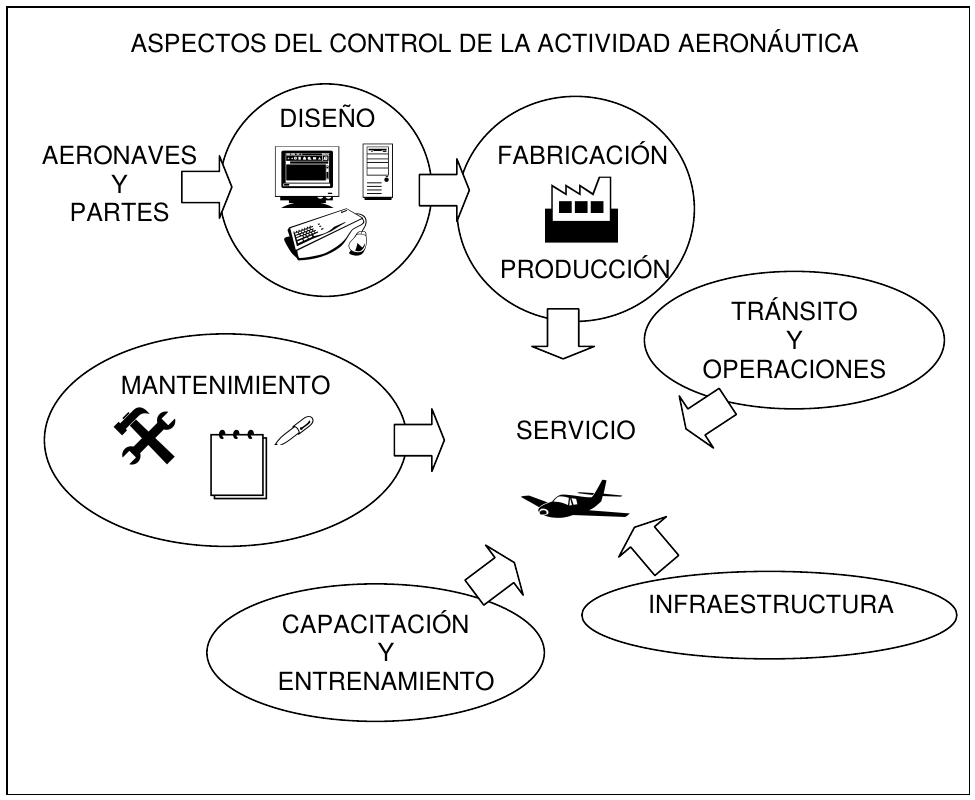
\includegraphics[width=1.00\linewidth]{figuras/fig_p089_38.png}
\end{center}

% ---- página 90 ----

\subsubsection*{LEGISLACIÓN AERONÁUTICA EN EL CAMPO INTERNACIONAL}
En la actividad aeronáutica los estados legislan sobre todos los actos relacionados con la actividad aeronáutica basándose en:

\begin{itemize}
  \item Códigos Aeronáuticos o equivalentes establecidos por Ley.
  \item La reglamentación de los Códigos Aeronáuticos.
\end{itemize}
\subsubsection*{CÓDIGOS AERONÁUTICOS DE LOS ESTADOS}
La Legislación básica contenida en los Códigos Aeronáuticos de los Estados comprende títulos referidos a aspectos tales como:

\begin{itemize}
  \item Personal Aeronáutico.
  \item La utilización de Espacio Aéreo.
  \item La infraestructura.
  \item Las Aeronaves.
  \item Los Accidentes de Aviación.
  \item Las Faltas y Delitos
  \item Etc.
\end{itemize}
Los Códigos Aeronáuticos suelen basarse, al menos en parte, en los Artículos del Convenio sobre Aviación Civil Internacional (Chicago 1944), al cual los Estados son miembros.

\subsubsection*{REGLAMENTACIÓN DE LOS CÓDIGOS AERONÁUTICOS}
Los títulos comprendidos en los Códigos Aeronáuticos son Reglamentados mediante Decretos Presidenciales y Resoluciones o Documentos equivalentes emitidos por la Autoridad competente, en base a:

\begin{itemize}
  \item Normas y Procedimientos o Métodos propios.
  \item Normas y Métodos recomendados en los Anexos al convenio sobre Aviación Civil Internacional (Chicago 1944).
\end{itemize}
\subsubsection*{CONTENIDO BÁSICO DE LOS REGLAMENTOS}
Un código o reglamento Aeronáutico debería contener Normas agrupadas homogéneamente, al menos en los siguientes Subtítulos:

\begin{itemize}
  \item Definiciones
  \item Reglas
  \item Aeronaves
  \item Personal Aeronáutico
  \item Tráfico Aéreo y Reglas de Operación General.
  \item Transportadores Aéreos y Operadores comerciales: Certificación y Operación.
  \item Escuelas y otras agencias certificadas.
\end{itemize}
Como ejemplos de reglamentaciones aeronáuticas tenemos: Las Regulaciones Federales de Aviación (FAR) contenidas en el Titulo XIV “Aeronáutica y Espacio” del Código de Regulaciones Federales de los Estados Unidos que administra la Administración Federal de Aviación (FAA), Los Joint Airworthiness Requirements (JAR) de las Joint Aviation Authorities (JAA) de la Unión Europea. Las RBHA de la Autoridad de Aviación Civil de Brasil.

\subsubsection*{LEGISLACIÓN AERONÁUTICA EN LA REPÚBLICA ARGENTINA}

% ---- página 91 ----

El Estado Argentino establece el sistema de control que se aplicara para establecer el cumplimiento de las normas y el régimen de castigos por su incumplimiento. En nuestro país se ha delegado la responsabilidad de legislar y la función de controlar la actividad aeronáutica a la Administración Nacional de Aviación Civil (ANAC) y a organismos civiles y profesionales.

La base legal de la Aeronáutica en nuestro país se encuentra contenida en:

\begin{itemize}
  \item El Código Aeronáutico de la Republica Argentina, establecido por la Ley Nro. 17.285.
  \item Regulaciones Argentinas De Aviación Civil (R.A.A.C.) (DISP. 57- 05) y sus anexos.
  \item El Decreto Nro. 4907/73. “Institución y Funcionamiento del Registro Nacional de Aeronaves”.
  \item El Decreto Nro. 2352//83 “Infracciones y Faltas Aeronáuticas”.
\end{itemize}
\subsubsection*{CONTENIDO DEL CÓDIGO AERONÁUTICO DE LA REPÚBLICA ARGENTINA}
\subsubsection*{I. GENERALIDADES}
II. CIRCULACIÓN AÉREA III. INFRAESTRUCTURA IV. AERONAVES V. PERSONAL AERONÁUTICO VI. AERONÁUTICA COMERCIAL VII. RESPONSABILIDAD VIII. BÚSQUEDA, ASISTENCIA Y SALVAMENTO IX. INVESTIGACIÓN DE ACCIDENTES DE AVIACIÓN X. SEGUROS XI. LEY APLICABLE, JURISDICCIÓN Y COMPETENCIA XII. FISCALIZACIÓN Y PROCEDIMIENTOS XIII. FALTAS Y DELITOS XIV. PRESCRIPCIÓN XV. DISPOSICIONES FINALES

\subsubsection*{REGULACIONES ARGENTINAS DE AVIACIÓN CIVIL (R.A.A.C.)}
Constituyen la reglamentación del Código Aeronáutico Argentino y se basan en la adopción y adaptación de las normas FAR de los EEUU, con excepción de las Partes 2 y VLA que responden a la JAR de la JAA. La Regulación esta conformado por nueve (9) Partes agregadas en los Anexos que integran la presente:

\textbf{Anexo I: Parte 61} “CERTIFICADOS DE IDONEIDAD AERONÁUTICA (LICENCIAS, CERTIFICADOS DE COMPETENCIA Y HABILITACIONES PARA PILOTOS”.

\textbf{Anexo II: Parte 63} “LICENCIAS PARA MIEMBROS DE LA TRIPULACIÓN – EXCEPTO PILOTOS”. \textbf{Anexo III: Parte 64} “CERTIFICADOS DE COMPETENCIA DE TRIPULANTES DE CABINA DE PASAJEROS”. \textbf{Anexo IV: Parte 65} “PERSONAL AERONÁUTICO (EXCEPTO MIEMBROS DE LA TRIPULACIÓN DE VUELO)”.

\textbf{Anexo V: Parte 67} “CERTIFICADO DE APTITUD PSICOFISIOLÓGICA”.

\textbf{Anexo VI: Parte 91}


% ---- página 92 ----

“REGLAS DE VUELO Y OPERACIÓN GENERAL”.

\textbf{Anexo VII: Parte 119} “CERTIFICACIÓN TÉCNICO OPERATIVA DE EXPLOTADORES DE SERVICIOS AEROCOMERCIALES”.

\textbf{Anexo VIII: Parte 121} “REQUERIMIENTOS DE OPERACIÓN: OPERACIONES REGULARES INTERNAS E INTERNACIONALES. OPERACIONES SUPLEMENTARIAS”.

\textbf{Anexo IX: Parte 135} “REQUERIMIENTOS DE OPERACIÓN: OPERACIONES NO REGULARES INTERNAS E INTERNACIONALES”

La permanente evolución tecnológica, las dificultades en servicio y los requerimientos operativos, entre otros aspectos, lleva a que permanentemente deban enmendarse las normas y aun sustituirlas, lo que demanda un gran esfuerzo al estado.

PROCEDIMIENTOS O MÉTODOS DEL REGLAMENTO DE AERONAVEGABILIDAD ARGENTINO

Los procedimientos (o Métodos) que establecen como se debe cumplir con lo prescripto en las Normas (Partes) contenidas en el Reglamento de Aeronavegabilidad, se emite en forma de:

\begin{itemize}
  \item Ordenes que constituyen MANUALES DE PROCEDIMIENTOS de aplicación obligatoria para la DA.
  \item Circulares de Asesoramiento que establecen Procedimientos aceptables para la autoridad aeronáutica, pero no únicos.
  \item Las Ordenes y Circulares de Asesoramientos de la DA se basan en la adopción y adaptación de las emitidas por la FAA de los EEUU. Con igual identificación y títulos en la mayoría de los casos.
  \item Asimismo la DA tiene vigentes Procedimientos emitidos en forma de: Disposiciones/DA del Director y Ordenes/DA del Director Nacional.
\end{itemize}
\subsubsection*{ORGANISMOS DE CONTROL DEL CUMPLIMIENTO DE LA REGULACIÓN}
\begin{itemize}
  \item DIRECCIÓN DE HABILITACIONES AERONÁUTICAS: Dependiente del Comando de
\end{itemize}
Regiones Aéreas, es el organismo encargado de otorgar las licencias y certificaciones al personal aeronáutico, certificar instituciones de capacitación y/o adiestramiento, y aprobar las operaciones que realizan las aeronaves.

\begin{itemize}
  \item DIRECCIÓN DE TRANSITO AÉREO: Dependiente del Comando de Regiones Aéreas, es
\end{itemize}
el organismo de control de la circulación aérea de aeronaves, proveer la información meteorológica, y emitir las publicaciones aeronáuticas.

\begin{itemize}
  \item DIRECCIÓN NACIONAL DE AERONAVEGABILIDAD: Dependiente del Comando de
\end{itemize}
Regiones Aéreas, es el organismo encargado de controlar la aptitud técnica del material aeronáutico y su mantenimiento, establecer las políticas de aeronavegabilidad que fueren necesarias para posibilitar el desarrollo seguro, regular y eficiente de la aviación civil de la República Argentina y vigilar su cumplimiento mediante la adopción de los sistemas y métodos


% ---- página 93 ----

de supervisión recomendados internacionalmente, a fin de contribuir al cumplimiento de las tareas del Organismo Superior.

\begin{itemize}
  \item JUNTA DE INVESTIGACIÓN DE ACCIDENTES DE AVIACIÓN: Dependiente del
\end{itemize}
Comando de Regiones Aéreas, este organismo tiene la función de determinar las causas de los accidentes de aviación y emitir recomendaciones a las autoridades aeronáuticas para prevenir nuevos accidentes.

\begin{itemize}
  \item REGISTRO NACIONAL DE AERONAVES: Dependiente del Comando de Regiones
\end{itemize}
Aéreas, es el organismo encargado de registrar la propiedad de la aeronaves, y otorgar las matriculas.

\begin{itemize}
  \item POLICÍA DE SEGURIDAD AEROPORTUARIA: Dependiente del Ministerio del Interior,
\end{itemize}
es el organismo encargado de la seguridad en las instalaciones aeroportuarias y las aeronaves mientras se encuentren dentro de esas instalaciones.

\begin{itemize}
  \item INSTITUTO NACIONAL DE MEDICINA AERONÁUTICA Y ESPACIAL: Dependiente
\end{itemize}
del Comando de Regiones Aéreas, es el organismo encargado de extender la aptitud médica al personal aeronáutico.

\begin{itemize}
  \item CONSEJO PROFESIONAL DE INGENIERÍA AERONÁUTICA Y ESPACIAL: Es el
\end{itemize}
organismo encargado de extender las matriculas para el ejercicio profesional, y regular la actividad profesional. Este organismo no pertenece a la Fuerza Aérea.

\begin{itemize}
  \item ORSNA: Es Organismo Regulador del Sistema Nacional de Aeropuertos debe asegurar el
\end{itemize}
\textbf{cumplimiento de los contratos de las empresas que tienen concesionados 36 de esos} \textbf{aeropuertos }(Aeropuertos Argentina 2000). Este organismo no pertenece a la Fuerza Aérea.

\begin{itemize}
  \item SUBSECRETARIA DE TRANSPORTE: Tiene la función de fiscalizar a las compañías
\end{itemize}
aéreas y autorizar a volar a los pilotos. Es la encargada de habilitar vuelos y rutinas aéreas. También recibe las denuncias de los usuarios.

\begin{itemize}
  \item ORGANIZACIÓN DE AVIACIÓN CIVIL INTERNACIONAL
\end{itemize}
Cuando las aeronaves comenzaron a surcar los cielos transportando pasajeros sobre otros países surgió la necesidad de establecer normas de seguridad internacionales que garantizaran a los habitantes de los estados la seguridad de las aeronaves de otros estados que circulaban por sus espacios aéreos. Con este fin se creó en Chicago (EEUU) la Organización de Aviación Civil Internacional (OACI) o conocida por sus siglas en ingles ICAO, cuyo objetivo es establecer un conjunto mínimo de exigencias que deben ser adoptados por los estados miembros en sus reglamentaciones aplicables a la actividad. Todos los países miembros que integran la OACI deben adoptar las recomendaciones que son emitidas por este organismo para garantizar que se cuenta con el mínimo de seguridad para que las aeronaves de estados miembros puedan sobrevolar otros estados miembros.

Como consecuencia de estos requerimientos mínimos en la seguridad, es que las regulaciones de los estados son similares, y no podría ser de otra manera, si fueran diferentes y algunas reglamentaciones fueran más permisivas que otras, implicaría que algunas aeronaves de algún estado miembro se requiriera menos seguridad que las exigidas para las aeronaves de otro estado, volando ambas sobre el mismo estado.


% ---- página 94 ----

\subsubsection*{CUESTIONARIO}
1. ¿Por qué la Argentina adopta las regulaciones FAR norteamericanas?

2. ¿En qué fecha se creó la OACI?

3. ¿Cuántos pises son miembros de OACI?

4. ¿Un mecánico que posee habilitación otorgada por la Autoridad Aeronáutica Argentina puede realizar mantenimiento sobre aeronaves matriculadas en otro estado?

5. ¿Un taller de mantenimiento habilitado por Autoridad Aeronáutica Argentina puede realizar mantenimiento sobre aeronaves matriculadas en otro estado?

6. ¿Quién es el responsable de garantizar la seguridad en la actividad aeronáutica de nuestro país?

7. ¿Quién emite la RAAC?

8. ¿Los procedimientos establecidos por el fabricante de la aeronave para el mantenimiento siempre son obligatorias para el operador de la aeronave?

9. ¿Quién puede conceder excepciones al cumplimiento de las RAAC?

10. ¿Qué organismo del estado habilita a los organismos o institutos para capacitar a personas para realizar el mantenimiento de aeronaves?

\textbf{Leer y responder:}

\textbf{Para ejercer como Técnico Aeronáutico o como Mecánico de Mantenimiento de Aeronaves, en el} \textbf{sector aeronáutico, debe estar matriculado en el Consejo Profesional de Ingeniería Aeronáutica y} \textbf{Espacial y además estar registrado en la Administración Nacional de Aviación Civil y para ejecutar} \textbf{tareas debe poseer licencia otorgada por la autoridad aeronáutica. Además debe advertirse que se} \textbf{le requerirá un certificado de aptitud psicofisiológica.}

1- ¿Cuál es la función de cada organismo mencionado en el párrafo anterior?

2- ¿Qué organismo otorga la aptitud psicofisiologica?

3- ¿Qué organismo de la autoridad aeronáutica otorga la licencia?

4- ¿Qué organismo otorga la matricula profesional?

Lectura Recomendada


% ---- página 95 ----

\begin{center}
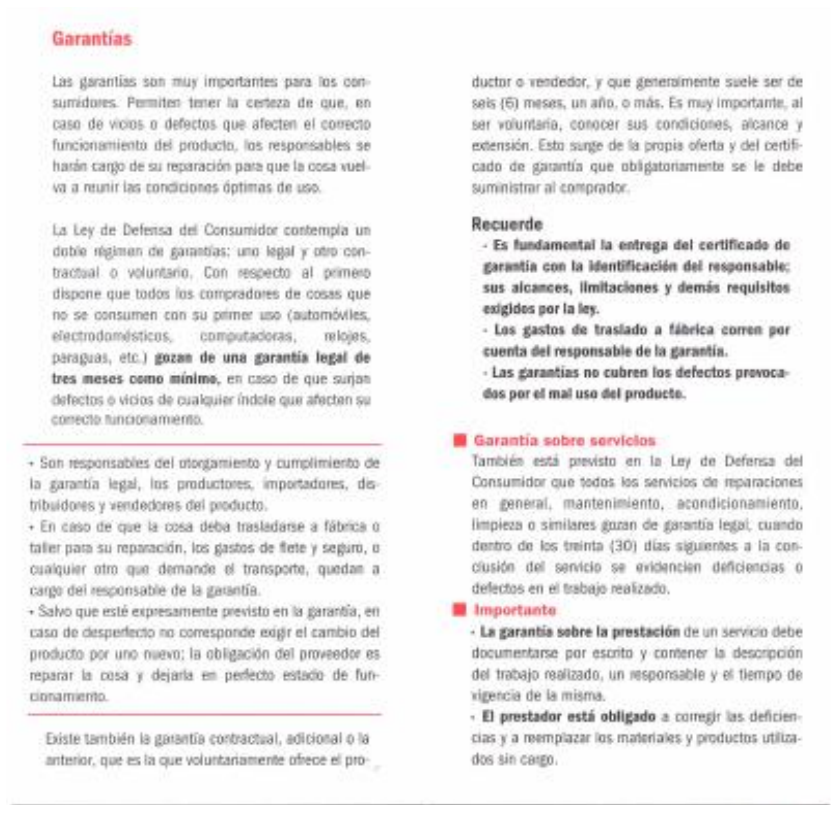
\includegraphics[width=0.86\linewidth]{figuras/fig_p095_39.png}
\end{center}

% ---- página 96 ----

\subsubsection*{CONTENIDOS DEL NÚCLEO TEMÁTICO SEXTO}
Mercadotecnia: Introducción, Concepto, funciones, nombre, logotipo, imagen, promoción, publicidad, marcas, etiquetas, empaque, canales de distribución.

\section*{MERCADOTECNIA}
\subsubsection*{INTRODUCCIÓN}
El productor debe intentar diseñar y producir bienes de consumo que satisfagan las necesidades del consumidor. Con el fin de conocer estas necesidades, se utilizan los conocimientos de la mercadotecnia. En un principio su área de acción se limitaba a intentar vender un producto que ya estaba fabricado, es decir, la actividad de la mercadotecnia era posterior a la producción del bien o servicio, y solo pretendía fomentar las ventas de un producto final ya conformado. Hoy la mercadotecnia tiene muchas más funciones que han de cumplirse antes de iniciarse el proceso de producción, entre ellas tenemos la investigación de mercados, diseño, desarrollo y prueba del producto.

La mercadotecnia o marketing, como también se la conoce, se concentra en analizar los gustos de los consumidores, pretende establecer sus necesidades y sus deseos e influir su comportamiento para que deseen adquirir los bienes y servicios ya existentes de forma que se desarrollan distintas técnicas encaminadas a persuadir a los consumidores para que adquieran un determinado producto.

Una de las ideas más importantes a tener en cuenta es el continuo cambio de gustos e intereses, los consumidores son cada vez más exigentes, tienen más educación, leen más, ven más televisión, escuchan más radio, viajan más que las generación anteriores y tienen más relaciones sociales. Sus demandas por lo tanto son más exigentes y sus gustos varían con mayor rapidez y se defienden de las publicidades agresivas. Las funciones de la mercadotecnia son asistidas por las ciencias sociales, la psicología y la sociología son las herramientas utilizadas para analizar la conducta de los consumidores, identifican los elementos claves en las inclinaciones de las personas, de sus necesidades, actividades, circunstancias, deseos, y motivaciones, que son los factores claves para entender los patrones de comportamiento de los consumidores.

\subsubsection*{CONCEPTO}
\textbf{Mercadotecnia o Marketing, se define como el conjunto de técnicas utilizadas para la} \textbf{comercialización y distribución de un producto entre los diferentes consumidores.} El intercambio de valores se viene considerando como el elemento central, es el denominador común de todas sus actividades. Su acción puede ser analizada desde diferentes puntos de vista, existiendo discrepancias respecto a su ámbito. Podemos distinguir varias dimensiones en el concepto:

Puede definirse como la comunicación que se establece entre al menos dos partes, con el objetivo de que una de ellas obtenga de la otra algo que valora, entregando a cambio algo que la otra parte aprecia. Cada una puede comunicar a la otra lo que tiene o desea y entregarlo. Además, existe libertad para aceptar o rechazar la oferta de la otra parte.

Su objetivo es tratar de conocer las necesidades genéricas del consumidor o carencias básicas propias de la naturaleza y condición humana, analizar los deseos o formas en que cada individuo


% ---- página 97 ----

desea satisfacer una necesidad determinada, estimular la conversión de los deseos en demanda buscando fórmulas creativas para potenciar la voluntad de compra y evitar las restricciones del poder adquisitivo.

La orientación de la empresa al mercado es el punto crucial de la mercadotecnia como actitud o filosofía. Todos los integrantes de la organización deben ser conscientes de la importancia del consumidor en la existencia, progreso y rentabilidad de la empresa.

Como función son las actividades encaminadas a alcanzar los objetivos de la organización descubriendo las necesidades de los clientes y tratando de satisfacerlos.

Como nivel agregado realiza dos funciones básicas: ajusta los flujos de producción y consumo y organiza las relaciones de intercambio en la sociedad. El encuentro eficiente entre la oferta y la demanda exige la organización de dos tipos de actividades:

I) La organización material del intercambio, de los flujos físicos de bienes desde el lugar de producción hasta el lugar de consumo (canales de distribución).

II) La organización de la comunicación, es decir, los flujos de información que deben preceder, acompañar y seguir al intercambio (promoción), con el fin de asegurar un encuentro eficiente entre la oferta y la demanda.

\subsubsection*{FUNCIONES}
\begin{itemize}
  \item La dirección de marketing tiene que tomar decisiones en relación al presupuesto publicitario,
\end{itemize}
tipo de publicidad e \textbf{imagen }que se quiere transmitir. Cuando la empresa decide utilizar una agencia de publicidad para la realización de los anuncios se precisa una selección de la agencia de publicidad y un contacto estrecho para la correcta selección de ejes de comunicación, realización de las piezas publicitarias, planificación de medios y planificación de las campañas publicitarias.

Las relaciones públicas se dirigen a múltiples públicos potenciales de la empresa, para conseguir la valoración de una imagen pública para la empresa. La gestión de la comunicación con los diferentes sectores de la opinión pública y la creación de un clima de confianza dentro y fuera de la empresa, constituyen áreas de gestión de las relaciones públicas.

\begin{itemize}
  \item La venta personal permite una comunicación adaptada al interlocutor, pudiendo ser la
\end{itemize}
persuasión más efectiva puesto que se realiza personalmente. Las decisiones relativas a la fuerza de ventas incluyen el reclutamiento y la selección de vendedores, su formación, el sistema de venta, la gestión de grupos de vendedores, asignación de territorios, rutas, plan de visitas, la retribución, motivación y control.

\begin{itemize}
  \item Las decisiones de marketing para que sean eficientes precisan de un sistema adecuado de
\end{itemize}
información comercial y de la necesaria coordinación entre las variables. Las variables comerciales no son independientes sino que interactúan por lo que se precisa una gestión conjunta que potencie sus resultados.

\subsubsection*{CREACIÓN DEL NOMBRE, LOGOTIPO, E IMAGEN DE LA EMPRESA}
NOMBRE DE LA EMPRESA El nombre de la empresa es su tarjeta de presentación, su sello distintivo y, por tanto, debe reunir una serie de características específicas; entre otras cosas debe ser:


% ---- página 98 ----

\begin{itemize}
  \item Descriptivo. El nombre, por sí mismo, debe reflejar el giro de la empresa y sus características distintivas de especialización.
  \item Original. La ley establece que el nombre de una empresa debe ser nuevo (que no exista ya en el mercado) y se puede constituir por cualquier signo o símbolo, palabra o palabras, figura, forma geométrica o tridimensional, o bien el nombre propio de una persona.
  \item Atractivo. El nombre debe ser llamativo y fácil de recordar; visible, esto es, que sea abundante en el lenguaje verbal común, para facilitar su aceptación y memorización.
  \item Claro y simple. Que se escriba como se pronuncia y viceversa.
  \item Significativo. Que se pueda asociar con diseños o frases representativas.
  \item Agradable. Una característica muy importante es que el nombre sea agradable, de buen gusto; que no implique dobles sentidos o términos vulgares, ya que esto provoca rechazo inmediato en el consumidor, aun cuando en un principio pudiera parecer gracioso.
\end{itemize}
Se agrega como ejemplo en la selección del nombre, un procedimiento de generación y evaluación de ideas utilizadas en las organizaciones para tomar decisiones llamado “Tormenta de ideas”.


\begin{center}
\small
\begin{tabular}{|p{\dimexpr0.100\linewidth-2\tabcolsep\relax}|p{\dimexpr0.134\linewidth-2\tabcolsep\relax}|p{\dimexpr0.123\linewidth-2\tabcolsep\relax}|p{\dimexpr0.125\linewidth-2\tabcolsep\relax}|p{\dimexpr0.119\linewidth-2\tabcolsep\relax}|p{\dimexpr0.147\linewidth-2\tabcolsep\relax}|p{\dimexpr0.126\linewidth-2\tabcolsep\relax}|p{\dimexpr0.091\linewidth-2\tabcolsep\relax}|}
\hline
\multicolumn{8}{|p{\dimexpr0.965\linewidth-2\tabcolsep\relax}|}{Realice una tormenta de ideas y determine cinco posibles nombres, según los atributos especificados} \\ \hline
\multicolumn{8}{|p{\dimexpr0.965\linewidth-2\tabcolsep\relax}|}{Atributo y calificación} \\ \hline
Nombre de la empresa & Descriptivo & Original & Atractivo & Claro & Significativo & Agradable & Total \\ \hline
XX & 2 & 3 & 2 & 3 & 2 & 3 & 15 \\ \hline
YY & 3 & 3 & 3 & 4 & 4 & 5 & 25 \\ \hline
ZZ & 4 & 3 & 3 & 4 & 4 & 3 & 24 \\ \hline
PP & 3 & 3 & 2 & 3 & 3 & 3 & 17 \\ \hline
\multicolumn{8}{|p{\dimexpr0.965\linewidth-2\tabcolsep\relax}|}{Nota: Calificar en una escala de 1 al 5} \\ \hline
\end{tabular}
\end{center}

\subsubsection*{LOGOTIPO}
El logotipo es la figura o símbolo específico representativo de la empresa o un producto, casi siempre se contrata a una agencia especializada en el área con el propósito de realizar su diseño en forma profesional para ser adoptado después por la empresa. Como se vio anteriormente, los símbolos utilizados por las organizaciones es registrable como Propiedad Industrial.

¿Identifica las organizaciones que tienen los siguientes logotipos?


\begin{center}

\includegraphics[width=0.16\linewidth]{figuras/fig_p098_42.png}
\end{center}

\begin{center}

\includegraphics[width=0.17\linewidth]{figuras/fig_p098_41.png}
\end{center}

\begin{center}

\includegraphics[width=0.20\linewidth]{figuras/fig_p098_40.png}
\end{center}

% ---- página 99 ----

\subsubsection*{IMAGEN}
La imagen es la forma en que la empresa es vista por el público. Algunos negocios pueden dirigir la mayor parte de su publicidad y promoción a la buena imagen de la compañía. Usted va a tener que decidir el monto que puede destinar al gastar para establecer, mejorar y mantener su imagen. Estos gastos pueden estar compensados por un incremento en sus ingresos.

\section*{PROMOCIÓN}
Promocionar es un acto de información, persuasión y comunicación, que incluye varios aspectos, como son: La publicidad, la promoción de ventas, las marcas, e indirectamente las etiquetas y el empaque. A partir de un adecuado programa de promoción, se puede lograr dar a conocer un producto así como incrementar el consumo del mismo.

\subsubsection*{PUBLICIDAD}
La publicidad implica una serie de actividades necesarias para hacer llegar un mensaje al mercado. Su objetivo principal es crear un impacto directo sobre el cliente para que compre un producto o servicio; con el consecuente incremento en las ventas. Para lograr esta meta, el empresario debe poner énfasis en:

\begin{itemize}
  \item Animar a los posibles compradores a buscar el producto que se les ofrece.
  \item Ganar la preferencia del cliente.
\end{itemize}
\textbf{Definimos la publicidad como una comunicación no personal y pagada, de promoción de} \textbf{ideas, bienes o servicios, que lleva a cabo un promotor identificado.}

La primera característica de la publicidad es ser \textbf{Comunicación}. Por tanto existe un Emisor, un Mensaje, un Medio y unos Receptores. La publicidad trata de comunicar un mensaje empleando diferentes Medios de Comunicación. La publicidad es comunicación Pagada\textbf{. }Si un periódico habla de nuestra empresa en un artículo no se trata de publicidad. Si el periódico dentro de una noticia o un artículo nos cita será porque nuestra empresa ha generado una noticia.

Diferenciamos la labor de Relaciones Públicas de lo que es Publicidad. Una de las actividades típicas de las Relaciones Públicas es conseguir que nuestra empresa aparezca en los medios de comunicación y aparezca de modo positivo. Una labor del departamento de Relaciones Públicas es enviar comunicados de prensa e información relevante a los periódicos, radios y televisiones sobre nuestra organización.

La publicidad trata de promocionar y por tanto de facilitar la labor de llevar esas ideas, bienes o servicios a los ciudadanos. Normalmente cuando se trata el tema de la publicidad lo primero que se piensa es en la publicidad de productos.

\textbf{Publicidad de Productos}. Es cierto que una parte importante de la publicidad es publicidad de productos. La publicidad de coches, detergentes o perfumes son un buen ejemplo de publicidad de productos.

\textbf{Publicidad de Servicios}. En las economías modernas cada vez adquieren más importancia los Servicios. Los bancos, los hospitales, las universidades, los abogados ofrecen servicios a la sociedad. A medida que la renta de un país se eleva una parte más importante de la economía la constituyen los servicios. Los bancos o las organizaciones de tarjetas de crédito publicitan sus


% ---- página 100 ----

servicios bancarios. Otro ejemplo de publicidad de servicios son las compañías telefónicas cuando anuncian sus servicios.

\textbf{También existe una publicidad que trata de promover Ideas}. Las campañas de publicidad en contra del tabaco, las de la Dirección de Tránsito para que los conductores tengan precaución o las campañas contra la droga son ejemplos de promoción de ideas. Otra cuestión es que algunas de las campañas contra las drogas son ejemplos de mala publicidad y en ocasiones no se sabe si están a favor o en contra.

\subsubsection*{PUBLICIDAD ENGAÑOSA}
La ley 22.802 de Lealtad Comercial, en su artículo 9, prohíbe cualquier clase de publicidad que mediante inexactitudes, imprecisiones u ocultamientos pueda inducir a error, engaño y/o confusión a los potenciales consumidores, respecto de las características, naturaleza, origen, calidad, precio, mezcla y condiciones de comercialización de los bienes muebles, inmuebles o servicios.

ELEMENTOS DE LA PUBLICIDAD.

Los elementos fundamentales que intervienen en la publicidad son:

\begin{itemize}
  \item El anunciante. Que paga la publicidad.
  \item El anuncio. El mensaje que se quiere difundir.
  \item Las agencias de publicidad. Las agencias de publicidad elaboran los mensajes. Buscan las mejores ideas y las transforman en anuncios para televisión, prensa, radio, u otros medios.
  \item Los medios de comunicación que son los vehículos para llevar la información. La televisión, la radio, Internet, volantes, afiches, la prensa son medios de comunicación.
  \item El público objetivo. El grupo poblacional que deseamos sea el receptor del mensaje.
\end{itemize}
LOS ANUNCIANTES.

El anunciante es en nombre de quien se realiza la publicidad. En los anuncios de Coca Cola el anunciante es la empresa Coca Cola. Los anunciantes más típicos son las empresas. Pero también realizan publicidad y son anunciantes la Organizaciones sin fines de lucro como la Cruz Roja Greenpace, las asociaciones y las Organizaciones Gubernamentales. Incluso las personas realizan publicidad cuando ponen un anuncio para vender su casa.

\begin{itemize}
  \item \textbf{Las empresas}. En muchos países la mayor parte de la publicidad es pagada por empresas que tratan de promover sus productos o servicios. Los fabricantes de automóviles tratan de promover sus modelos y los servicios que ofrecen.
  \item \textbf{Las Organizaciones sin fines de lucro}. Son organizaciones sociales que no tratan de obtener beneficios empresariales sino promover iniciativas, y necesitan comunicarse con la sociedad. Distintas organizaciones tratan de conseguir dinero para ayudar a los pobres, los huérfanos, para defender el medio ambiente o promocionar las más diversas causas. Las Organizaciones no lucrativas realizan actividades de marketing para conseguir sus objetivos que pueden ser muy diversos. La captación de personal o voluntarios, la difusión de sus ideas, la defensa de unos ideales, la obtención de recursos por parte de las organizaciones puede requerir la realización de publicidad.
  \item \textbf{Las organizaciones sociales}. Los partidos políticos, los sindicatos, las asociaciones de empresarios, las organizaciones gremiales y todo tipo de asociaciones tratan de promoverse empleando el marketing y realizando comunicación comercial o publicidad.
\end{itemize}

% ---- página 101 ----

\begin{itemize}
  \item \textbf{Las Administraciones Públicas}. Los ejércitos para contratar militares, las Agencias del Gobierno, los Gobiernos Locales y numerosos Organismos Públicos realizan de forma habitual campañas publicitarias.
  \item \textbf{Las personas}. Si ponemos un anuncio en el periódico local para vender nuestro auto o nuestra casa estamos haciendo publicidad. El mago, el cantante especialista en Bodas, Bautizos y Comuniones, el abogado pueden emplear la publicidad para ofertar sus servicios a la comunidad.
\end{itemize}
En algunos países se encuentra muy regulada e incluso prohibida la publicidad de ciertos profesionales como abogados y médicos. En otros países como los Estados Unidos es normal que los abogados y las firmas de abogados se promociones empleando anuncios pagados en medios de comunicación.

\subsubsection*{LOS MEDIOS DE COMUNICACIÓN}
Cuando los anunciantes dan a conocer información sobre los productos o servicios que ofrece, utiliza algunos medios, como son:

\begin{itemize}
  \item Periódicos y revistas. Cubren con su circulación un territorio geográfico seleccionado (parte de una ciudad, una ciudad completa, varias poblaciones vecinas o un número de regiones adyacentes). Además, los anuncios en los periódicos y revistas llegan a personas de casi todos los estratos económicos. Es necesario, al seleccionar este medio, identificar cuál periódico o revista es más leído por un estrato determinado y cuál sección del mismo. La ventaja de este medio es que se conoce el número de periódicos que se venden y de forma bastante aproximada el número de lectores.
  \item Anuncios Publicitarios: El anuncio publicitario es otro medio que tiene por objeto motivar al cliente potencial a comprar el producto o servicio de la empresa, por lo que dicho anuncio debe incluir: El dibujo del producto o su equivalente, las palabras del mensaje (atractivo, cualidades del producto o servicio) y nombre de la empresa y producto (dirección y teléfono).
  \item Radio y Televisión. La radio y Televisión son accesibles a todo lo largo y ancho de los países (la mayor parte de los hogares poseen radios y televisión y la radio está en la mayoría de los vehículos de transporte). Por tanto estos medios ofrece la oportunidad de una exposición masiva de los mensajes publicitarios. Este medio publicitario también puede estar dirigido a un mercado particular, en un poblado o ciudad específica mediante la selección adecuada del mensaje y de la estación. Estos medios suelen tener la dificultad de que se desconoce cuántos son los espectadores reales de estos medios. En algunos casos gastar un poco de dinero en un medio con muy pocos espectadores puede ser una pérdida de dinero.
  \item Volantes. Los volantes son por lo general distribuidos por los dueños o empleados en las pequeñas empresas, de puerta en puerta, en colonias seleccionadas, en puntos de reunión del segmento de mercado seleccionado; su impacto puede ser muy fuerte, siempre y cuando se cuide el contenido y presentación de los mismos.
  \item Internet. Internet se ha convertido en un nuevo medio publicitario que permite medir con exactitud el número de personas que reciben el mensaje. Internet permite dirigir el mensaje a grupos de personas muy definidos.
\end{itemize}

% ---- página 102 ----

\begin{itemize}
  \item La Publicidad Exterior. Una parte importante de la publicidad es la publicidad mediante vallas publicitarias, cabinas de teléfono y en general todos los diferentes carteles, rótulos y elementos publicitarios en las calles, carreteras y espacios públicos.
\end{itemize}

\begin{center}
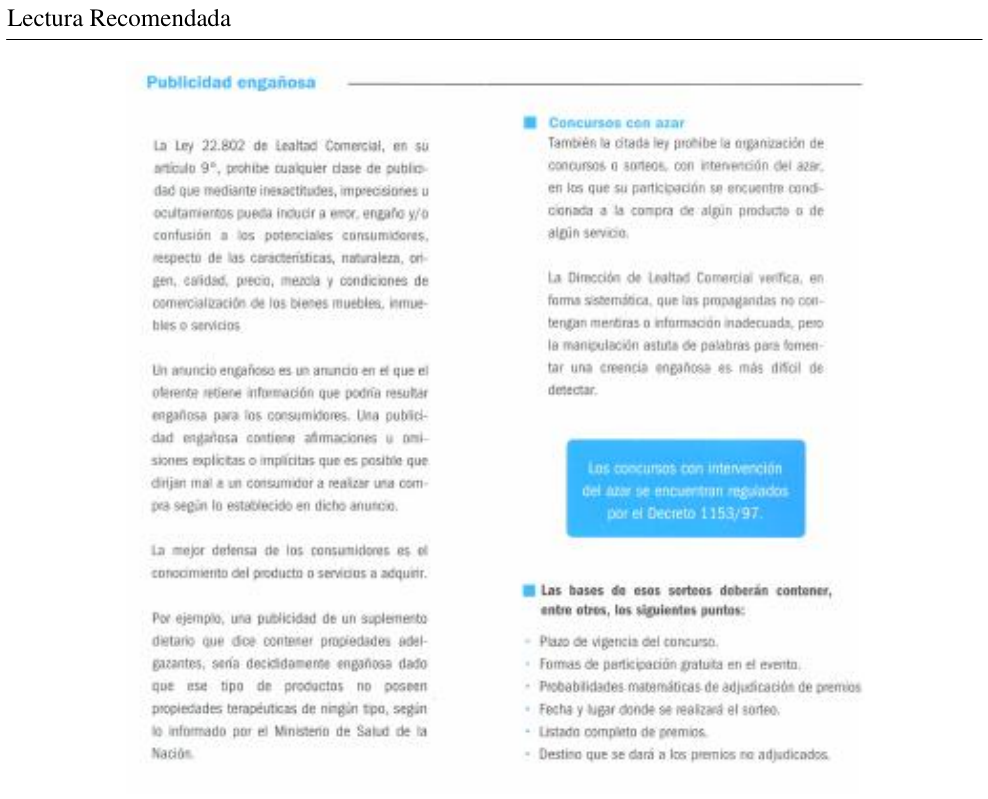
\includegraphics[width=1.00\linewidth]{figuras/fig_p102_43.png}
\end{center}

\subsubsection*{PROMOCIÓN DE VENTAS}
Otro elemento que puede causar un gran impacto en el mercado, es el sistema de promoción de ventas que se lleve a cabo; la promoción de ventas comprende actividades que permiten presentar al cliente con el producto o servicio de la empresa; la promoción de ventas debe llevarse a cabo para que el cliente ubique al producto o servicio de la empresa en el mercado. La promoción de ventas la constituyen actividades que tratan de proporcionar incentivos para la venta e incrementar el valor ofrecido al consumidor. La promoción de ventas suele constituir una acción limitada en el tiempo y que generalmente pretende incrementar las ventas a corto plazo. Representa una parte significativa del presupuesto de las actividades reforzadoras de la oferta. La utilización de los instrumentos promocionales precisa \textbf{creatividad }junto con una cuidadosa gestión y \textbf{planificación}. Los sorteos, regalos y cupones de descuento constituyen promociones que pueden dirigirse a los consumidores, los intermediarios y la fuerza de ventas.

Ejemplo de estas actividades son: muestras gratis, regalos en la compra del producto, concursos o sorteos (se encuentran regulados por el decreto 1153/97), ofertas de introducción, patrocinio y/o participación en eventos sociales, educativos, culturales, deportivos o presentación en ferias, entre otros.


% ---- página 103 ----

\subsubsection*{MARCAS}
La venta de un producto o servicio se facilita cuando el cliente lo conoce y lo solicita por su nombre. Esto es posible gracias a las marcas. Una marca es un nombre, término, signo, símbolo o diseño, o combinación de los mismos, que identifican los bienes y/o servicios que ofrece una empresa y señala una clara diferencia con los de su competencia.

Otros elementos que contribuyen a diferenciar al producto o servicio de la empresa, de los ofrecidos por otras organizaciones, son el logotipo (figura o símbolo específico y original) y el eslogan (frase o grupo de palabras, también originales, que presentan la imagen de la empresa o producto de la misma). Las marcas están sujetas a condiciones para su conservación, estas condiciones están reglamentadas en la Ley de la Propiedad Industrial.

\subsubsection*{ETIQUETA}
Son las formas impresas que lleva el producto para dar información al cliente acerca de su uso o preparación. Las etiquetas deben dar a conocer las características, usos, presentación y materias primas con que fue elaborado el producto. Las etiquetas no sólo son exigidas por ley; sino que pueden jugar un papel importante en la imagen que el consumidor construya del producto, por tanto, es necesario diseñarlas con mucho cuidado y detenimiento. En el Instituto Nacional de la Propiedad Industrial (INPI) con domicilio en Avda. Paseo Colón 717, 2° piso (1063) Buenos Aires -República Argentina se registran las autorizaciones de marcas, nombres comerciales, patentes, y otras formas de propiedad industrial conforme a lo estudiado anteriormente en Marcas y Patentes.

\subsubsection*{EMPAQUE}
El empaque debe ayudar a vender el producto, sobre todo el que es adquirido directamente por el consumidor final. No basta que el empaque muestre el nombre del fabricante y la marca, el recipiente también debe servir como medio publicitario, aumentando el valor del producto ante el cliente; además se debe buscar que sea reciclable y, si es posible, biodegradable.

\subsubsection*{CANALES DE DISTRIBUCIÓN}
Cuando hablamos de distribución comercial nos referimos a la gestión de un amplio conjunto de actividades para llevar el producto desde la fábrica al consumidor. Tratamos de responder a las preguntas de ¿Cómo llevar el producto al cliente? y ¿Cómo vender más?

El gran desarrollo industrial del siglo XIX y XX fue posible gracias a la mejora de los sistemas de transportes. El desarrollo del transporte marítimo, por carretera y del ferrocarril permitiría a los fabricantes llegar con un bajo coste y de forma rápida a un gran número de consumidores. Al mejorar los sistemas de transportes las empresas pueden acceder a mercados muy amplios. Y el poder acceder a grandes mercados es lo que impulsa la producción en masa y las economías de escala. Otro avance importante se produce con la mejora de los sistemas de conservación y almacenamiento de los productos. La mejora en los sistemas de conservación de productos alimentarios permite ampliar el mercado de los productos agrícolas y ganaderos.

Las principales decisiones en el proceso de diseño y \textbf{selección del canal de distribución }se relacionan con la longitud del canal, el número de intermediarios a utilizar, el tipo específico de intermediario y las responsabilidades de cada integrante del canal. Partiendo de los objetivos fijados y en función de las características del entorno la dirección comercial selecciona el canal de distribución y los intermediarios concretos de los distintos escalones de la red de distribución. El importante coste que representa para muchas empresas y la necesidad de acceder a los mercados en el momento del tiempo y en las condiciones que los clientes demandan, hacen de la \textbf{distribución física }una actividad esencial. La distribución física requiere la toma de decisiones y


% ---- página 104 ----

la gestión de los pedidos, la organización y localización de almacenes, la gestión de existencias y de medios de transporte. Las decisiones en esta área toman en consideración los costes, el tiempo de entrega, la capacidad, la disponibilidad y la estrategia establecida de servicio a los clientes. De especial importancia es la gestión de las relaciones con la distribución. El establecimiento de \textbf{canales de información }y la colaboración de los distintos niveles de la cadena de generación de valor del producto son esenciales para responder de forma flexible y rápida a las cambiantes demandas de los consumidores finales. Igualmente la cooperación entre los distintos niveles de la cadena productiva es un factor esencial en la reducción de costes y en la disminución de los tiempos de entrega.

\subsubsection*{ACCESO A LOS CANALES DE DISTRIBUCIÓN}
Para los que desean ingresar, se puede crear una barrera, por la necesidad de asegurar la distribución de su producto o servicio, debido al grado en que los canales lógicos de distribución para el artículo, han sido previamente utilizados por las empresas establecidas, por lo que la nueva empresa deberá persuadir a los canales de que acepten su producto o servicio mediante la reducción de precios, asignaciones para publicidad compartida y similares, lo cual reduce las utilidades.

Lectura Recomendada


% ---- página 105 ----

\begin{center}
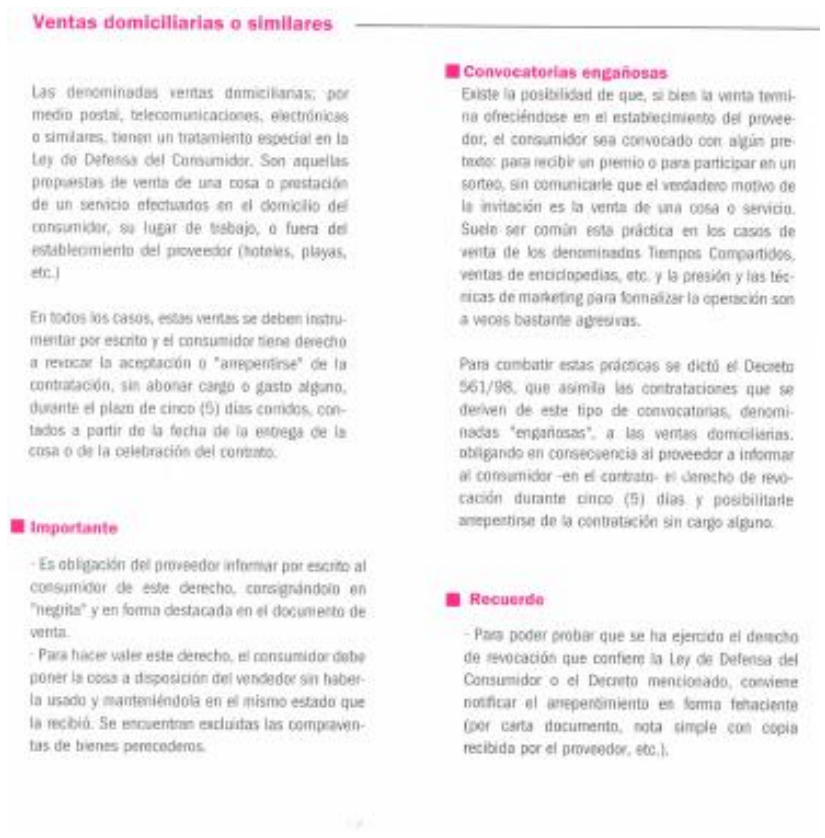
\includegraphics[width=0.84\linewidth]{figuras/fig_p105_44.png}
\end{center}

% ---- página 106 ----

\subsubsection*{CONTENIDOS DEL NÚCLEO TEMÁTICO SÉPTIMO}
Capacitación: Introducción, concepto, tipos de capacitación. Ventajas y Desventajas. Objetivos. Las necesidades de capacitación. Información: Concepto, La importancia de la información en la empresa, Fuentes de información en la empresa, operaciones, ciclo de vida, atributos de la información. Administradores de la información.

\section*{CAPACITACIÓN}
\subsubsection*{INTRODUCCIÓN}
Los empleados competentes no lo serán siempre. Su habilidad se puede deteriorar, la tecnología puede volver obsoletas sus habilidades, la organización puede ingresar a nuevas áreas, cambiando su tipo de trabajo y habilidades necesarias para realizarlas.

Aunque la capacitación auxilia a los miembros de la organización a desempeñar su trabajo actual, sus beneficios pueden prolongarse a toda su vida laboral y pueden auxiliar en el desarrollo de las personas capacitadas para cumplir futuras responsabilidades.

La capacitación en todos los niveles constituye una de las mejores inversiones en recursos humanos y una de las principales fuentes de bienestar para el personal de toda la organización.

\subsubsection*{CONCEPTO}
Entendemos por capacitación la transferencia de conocimientos y habilidades al personal de una organización, para cubrir las necesidades de su actual puesto de trabajo y la demanda de su plan de carrera. Se considera como un proceso educativo a corto plazo que utiliza un procedimiento planeado, sistemático y organizado, mediante el cual el personal de una empresa adquiere los conocimientos y habilidades técnicas necesarias para acrecentar la eficacia en el logro de los objetivos organizacionales.

\subsubsection*{TIPOS DE CAPACITACIÓN}
\begin{itemize}
  \item Capacitación natural: Es aquella que se origina adentro del grupo, es decir, a la que es
\end{itemize}
producto del intercambio de experiencias o es el fruto de la creatividad de alguno de sus integrantes que luego se trasmite a los otros.

\begin{itemize}
  \item Capacitación Inducida: Cuando ella proviene de las enseñanzas de una persona extraña al
\end{itemize}
grupo. Ejemplo: Los cursos que suelen dictarse en las empresas.

\subsubsection*{VENTAJAS Y DESVENTAJAS}
El primer tipo de capacitación es la más efectiva, porque el personal se siente más cercanamente vinculada a la cuestión tratada en tanto que la capacitación inducida por lo general es impuesta por la dirección empresaria por lo que el personal, con bastante frecuencia la toma sin mucho interés. En este último caso, el objetivo proyectado y deseado deberá ser programado como una comunicación personal. En otras palabras tendrá que ser dirigida a grupos relativamente pequeños y teniendo en cuenta el interés laboral particular de sus componentes.

Otros de los puntos que deben ser tenido en cuenta sobre este particular, es que la capacitación puede resultar un arma de doble filo para aquellas empresas que la organizan pretendiendo elevar la productividad o la mejor atención al cliente, si paralelamente, no introduce los modernos conceptos de las relaciones públicas en su gestión empresarial.

No debe olvidarse que cuando más capacitada sea una persona, más exigente será por lo que deben implantarse conjuntamente la política de capacitación con la de satisfacción de recursos humanos. Por tales razones y en otras palabras, queremos resaltar que todo programa de


% ---- página 107 ----

capacitación debe adecuarse en forma paralela a la introducción de una política de relaciones públicas interna.

\subsubsection*{OBJETIVOS DE LA CAPACITACIÓN}
I. \textbf{Productividad}: Las actividades de capacitación y desarrollo no solo deberían aplicarse a los empleados nuevos sino también a los trabajadores con experiencia. La instrucción puede ayudarle a los empleados a incrementar su rendimiento y desempeño en sus asignaciones laborales actuales.

II. \textbf{Calidad}: Los programas de capacitación y desarrollo apropiadamente diseñados e implantados también contribuyen a elevar la calidad de la producción de la fuerza de trabajo. Cuando los trabajadores están mejor informados acerca de los deberes y responsabilidades de sus trabajos y cuando tienen los conocimientos y habilidades laborales necesarios son menos propensas a cometer errores costosos en el trabajo. III. \textbf{Planeación de los Recursos Humanos}: La capacitación y desarrollo del empleado puede ayudar a la compañía y a sus necesidades futuras de personal.

IV. \textbf{Prestaciones indirectas}: Muchos trabajadores, especialmente los gerentes consideran que las oportunidades educativas son parte del paquete total de remuneraciones del empleado. Esperan que la compañía pague los programas que aumenten los conocimientos y habilidades necesarias.

V. \textbf{Salud y Seguridad}: La salud mental y la seguridad física de un empleado suelen estar directamente relacionados con los esfuerzos de capacitación y desarrollo de una organización. La capacitación adecuada puede ayudar a prevenir accidentes industriales, mientras que en un ambiente laboral seguro puede conducir actividades más estables por parte del empleado.

VI. \textbf{Prevención de la Obsolescencia}: Los esfuerzos continuos de capacitación del empleado son necesarios para mantener actualizados a los trabajadores de los avances actuales en sus campos laborares respectivos.

La Obsolescencia del empleado puede definirse como la discrepancia existente entre la destreza de un trabajador y la exigencia de su trabajo.

La Obsolescencia puede controlarse mediante una atención constante al pronóstico de las necesidades de recursos humanos, el control de cambios tecnológicos y la adaptación de los individuos a las oportunidades así como los cambios tecnológicos.

VII. \textbf{Desarrollo Personal}: No todos de los beneficios de capacitación se reflejan solamente en la empresa. En el ámbito personal los empleados también se benefician de los programas de desarrollo administrativos, les dan a los participantes una gama más amplia de conocimientos, una mayor sensación de competencia y un sentido de conciencia, un repertorio más grande de habilidades y otras consideraciones, son indicativas del mayor desarrollo personal.

\subsubsection*{ANÁLISIS DE LAS NECESIDADES DE CAPACITACIÓN}
Las necesidades de capacitación dentro de una organización deben contener tres tipos de análisis:

\begin{itemize}
  \item Análisis de Organizaciones: Se centra principalmente en la determinación de los objetivos
\end{itemize}
de la empresa, sus recursos y la localización de éstos y sus relaciones con el objetivo.

\begin{itemize}
  \item Análisis de Funciones: Se enfoca sobre la tarea o el trabajo, sin tomar en cuenta el
\end{itemize}
desempeño del empleado en el mismo.

\begin{itemize}
  \item Análisis de Personas: Examina el conocimiento, las actitudes y las habilidades del individuo
\end{itemize}
que ocupa cada puesto y determina que tipos de conocimientos, actitudes o habilidades debe


% ---- página 108 ----

adquirir y que tipos de modificaciones deben hacer a su comportamiento. La determinación de las necesidades de capacitación sobre la base de los análisis de funciones se revela las capacidades que debe tener cada individuo dentro de la administración, en términos de liderazgo, motivación, comunicación, dinámicas de grupos, relación de conflictos, implantación de cambios.

Una vez determinada las necesidades de capacitación, se eligen los métodos (conferencias, reuniones de grupos, cursos, análisis de casos, etc.) de acuerdo a las posibilidades que tengan para proporcionar la capacitación necesaria.

\subsubsection*{LA CAPACITACIÓN EN LAS EMPRESAS}
La capacitación en las empresas se produce habitualmente en un contexto socioeconómico, organizacional y de relaciones socialmente complejo, en el que intervienen múltiples actores. Bajo las restricciones del mercado y los riesgos que genera la competitividad se expresan diversas necesidades, entre ellas la de capacitación. Esta no aparece como un proceso natural, sino que al estar concebida como un instrumento de cambio es un recurso, entre otros, de la dirección de la empresa. Para la empresa la capacitación debe proveer comportamientos y conocimientos que posibiliten aplicar exitosamente una nueva tecnología, y/u organización de la producción y en numerosos casos se trata de responder a estas exigencias a corto plazo. La demanda de capacitación proviene de la acción, el tipo de participación es voluntaria, sus objetivos son negociados y la empresa puede recurrir a ella tanto para prever situaciones, ante los riesgos que genera la presión del mercado, como para responder a los cambios del aparato productivo y a la necesidad de contar con calificaciones específicas. Desde esa óptica, los procesos de capacitación, remiten a un tipo de intervención cuyos efectos se reflejan en los individuos y en la estructura de la propia organización. Como toda acción educativa, es inductora de cambios personales y transformadora de la organización ya que todo proyecto de formación intenta generar mutaciones en las actitudes, en la manera de percibir y esto redunda directamente en la cultura organizativa.

Por otra parte, para que un programa de entrenamiento se sostenga, tiene que adaptarse a esa cultura. Se trata al mismo tiempo de una acción transformadora y de ruptura que se corresponde con un ciclo de adaptación del que puede resultar un equilibrio que posibilita confrontar un cambio.

\subsubsection*{CAPACITACIÓN EN EL TRABAJO}
La capacitación directa sobre el puesto de trabajo se imparte durante las horas de trabajo y se emplea básicamente para enseñar a las personas a desempeñar su puesto actual.

En las instrucciones directas sobre el puesto de trabajo se distinguen varias etapas. En primer lugar, se brinda a la persona una descripción general del puesto, su objetivo y los resultados que se esperan de él, destacándola importancia de la capacitación. A continuación el capacitador efectúa un trabajo a fin de proporcionar un modelo. De esta manera la persona puede transferir los conocimientos a su puesto de trabajo.

Las continuas demostraciones proporcionan la ventaja de la repetición y de la retroalimentación. Finalmente se pide a la persona que lleve a cabo la labor sin supervisión.

\subsubsection*{CAPACITACIÓN FUERA DEL TRABAJO}
Las clases en aulas: son ideales para transmitir información específica. Son muy eficaces para desarrollar habilidades técnicas y para resolver problemas.


% ---- página 109 ----

Las películas: Se pueden usar para enseñar de manera explícita, habilidades técnicas que no son fáciles de transmitir mediante otros métodos. Tienden a depender más de la comunicación y menos de la imitación y la participación activa.

Ejercicios de simulación: A fin de evitar que la capacitación interfiera con las operaciones normales de las organizaciones o reducir los costos o los riesgos se utilizan instalaciones que simulan las condiciones de operación real. Enseña la habilidad para resolver problemas.

\subsubsection*{CAPACITACIÓN EN LAS EMPRESAS AERONÁUTICAS}
La reglamentación Argentina exige a los explotadores aeronáuticos un programa de capacitación para el personal técnico que puede clasificarse en dos grupos:

\begin{itemize}
  \item CAPACITACIÓN SOBRE PROCEDIMIENTOS INTERNOS DE LA EMPRESA:
\end{itemize}
El contenido trata sobre las políticas internas de la organización, la utilización de los manuales, procedimientos del mantenimiento, el uso de los formularios.

\begin{itemize}
  \item CAPACITACIÓN TÉCNICA DE MANTENIMIENTO Y DE INSPECCIÓN:
\end{itemize}
Puede ser una combinación de instrucción en aula y en el puesto de trabajo (on job-training), y está dirigido al personal técnico. En las empresas aeronáuticas suele adoptarse para el dictado de estos cursos de capacitación, el ATA 104 (Air Transport Association). El ATA 104 clasifica la capacitación según niveles que van del I al V según la siguiente descripción del cuadro:


\begin{center}
\small
\begin{tabular}{|p{\dimexpr0.138\linewidth-2\tabcolsep\relax}|p{\dimexpr0.862\linewidth-2\tabcolsep\relax}|}
\hline
NIVELES & DESCRIPCIÓN \\ \hline
NIVEL I & Es un curso de familiarización general para el personal jerárquico de la empresa. Se dicta a requerimiento y trata de una descripción breve de cada sistema de la aeronave. Este nivel contiene 12 horas. \\ \hline
NIVEL II & Es un curso de rampa y tránsito, sistemas, planta de poder, electricidad, y aviónica. está dirigido al personal de base y escalas que atienden al despacho de la aeronave y realiza inspecciones diarias y transito. Consta de 60 horas. \\ \hline
NIVEL III & En este nivel existen dos especialidades de curso. Un curso es de sistemas, planta de poder, electricidad, y aviónica dirigido al personal de base y línea de la especialidad mecánicos, el otro es un curso de electricidad, aviónica, planta de poder, y sistemas dirigido al personal de base y línea de la especialidad electricista y radio. La duración es de 120 horas. \\ \hline
NIVEL IV & Son cursos específicos de algún sistema o equipo especial en el cual se necesita una instrucción adicional no contemplada en el nivel III, por ejemplo: Pruebas, comprobaciones, análisis de fallas. \\ \hline
NIVEL V & Son cursos de recorrida general de componentes realizados en las fábricas de aviones, motores o del propio componente. Este curso está dirigido al personal especializado. \\ \hline
\end{tabular}
\end{center}

Estos cursos pueden ser de carácter INICIAL cuando son recibidos por primera vez. Luego de transcurridos entre 24 y 36 meses de haber recibido el nivel inicial, se dictan cursos RECURRENTES (refresco) según los requerimientos de la empresa, con el objetivo de corregir deficiencias de cualquier capacitación anterior, actualizarla y reforzarla. Los cursos se dictan por ATA o los ATA relacionados con algún sistema.

\subsubsection*{LOS RESPONSABLES}
En cuanto al ámbito propio del que depende la capacitación, existen diferencias según el tamaño y el sector de actividad. En empresas Pyme del sector comercio y del sector servicios, la responsabilidad recae en el área de personal aunque a medida que disminuye el tamaño dentro del estrato está en manos de sus directores, propietarios o socios, siendo para las empresas del


% ---- página 110 ----

sector servicios el ámbito en que esta categoría presenta el mayor peso relativo. En las empresas grandes, la capacitación depende exclusivamente de las áreas de recursos humanos y de personal y en las de mayor dimensión, es formulada en el marco de una estrategia general que formalmente procura respaldar y fomentar la formación de los empleados para que puedan alcanzar los estándares de competencia requeridos, y desarrollar su potencial.

\section*{INFORMACIÓN}
\subsubsection*{INTRODUCCIÓN}
A partir de la existencia de redes internacionales de información y la posibilidad de obtenerla, ésta ha pasado a ser una materia prima más que hace funcionar nuestra empresa y nuestra sociedad. Un mundo globalizado significa que sus competidores pueden estar en cualquier rincón de este planeta. Las empresas del mundo industrializado han comprendido muy pronto que es la información que les otorga una ventaja significativa sobre sus competidores.

¿Qué es Información?

ALGUNAS DEFINICIONES

1. Diseño de Sistemas de Información (Burch-Grudnitski) La información la componen datos que se han colocado en un contexto significativo y útil y se ha comunicado a un receptor, quien la utiliza para tomar decisiones.

2. Sistemas de Información Gerencial (Gordon B. Davis) La información es un dato que ha sido procesado en una forma significativa para el receptor y su valor es real o percibido actualmente o en acciones prospectivas o en decisiones.

3. Análisis y Diseño de Sistemas de Información: (James A. Senn) Conjunto de datos que dentro de contexto significativo y útil, ésta se comunica a un receptor, quien la utiliza para tomar decisiones.

4. Enciclopedia Británica En lo general el término información se refiere a los factores y opiniones enviadas y recibidas durante la vida diaria. Se obtiene información directamente de otras personas, medios masivos, bancos de datos y de todos los fenómenos que observamos en el ambiente.

5. Teoría General de Sistemas (John P- Van Gigh) Grados de libertad que existen en una situación específica para elegir entre señales, símbolos, mensajes o patrones a trasmitirse, que permiten la elaboración de un concepto.

6. Sistemas de Información administrativa. (Robert G. Murdick) Es un signo o conjunto de signos que impulsan a la acción. Se distingue de los datos, porque estos no son estímulos de la acción, si no simplemente cadenas de caracteres o patrones sin interpretar.

7. Análisis y Diseño de Sistemas. (Kendall y Kendall) Elemento decisivo que en un momento dado determina el éxito o fracaso del negocio ya que no es un producto exclusivamente colateral de la operación de la empresa, sino que es si, es uno de los promotores de la misma.

8. Administración (David R. Hampon) La base de toda información son los datos, los hechos que describen una entidad. Los datos se convierten en información al procesarlos y darles una forma significativa. La información es en realidad, datos transformados para comunicar un significado o conocimiento.

9. Administración de Organizaciones. (Fremont E. Kast y James E. Rosenzweig)


% ---- página 111 ----

Es la sustancia de los sistemas de comunicaciones, en sus diversas formas (impulsos electrónicos, palabras escritas o habladas, informes formales), la información es un ingrediente básico para la toma de decisiones. Aumenta nuestros conocimientos y podría llevar a cambio en creencias, valores y actitudes.

Alumnos de Sistemas de Información:

Es obtener y conocer los datos suficientes de una determinada situación o problema, de tal manera que se tengan las bases suficientes para formarse un concepto y tomar un curso de acción, elegir o tomar una decisión determinante.

\subsubsection*{LA IMPORTANCIA DE LA INFORMACIÓN EN LA EMPRESA}
¿Cuáles son las características del entorno actualmente?

\begin{itemize}
  \item La globalización
  \item La demanda más selectiva
  \item Los ciclos de los productos más cortos
  \item Síntesis: cambio
\end{itemize}
¿Qué implicaciones tiene para la empresa?

\begin{itemize}
  \item Exige una nueva forma de hacer negocios
  \item Hace que la información sea clave –La externa (competidores, clientes, tecnología) –La interna
\end{itemize}
¿Cuáles son los 3 factores productivos básicos al que ahora se une la información?

La tierra, capital y trabajo (¿informática?)

¿Qué características peculiares tiene este recurso? ¿Qué consecuencias tienen?

Es un bien público:

–no desgaste: No se consume con el uso, sino que incluso en su caso incrementa su valor –no exclusión: No es apropiable fácilmente No es fácilmente divisible Combinada da lugar a más información Las técnicas de gestión de recursos han de adaptarse

\subsubsection*{FUENTES DE INFORMACIÓN EN LAS EMPRESAS}

\begin{center}
\small
\begin{tabular}{|p{\dimexpr0.181\linewidth-2\tabcolsep\relax}|p{\dimexpr0.819\linewidth-2\tabcolsep\relax}|}
\hline
Activos fijos & Valoración/ costos de mantenimiento/ reparación / actualización/ sustitución. Modelos de simulación de financiación (compra, leasing, alquiler), Modelos de simulación de funcionamiento \\ \hline
Compras & Lanzamiento automático de pedidos / información sobre proveedores / selección de ofertas / control de calidad / rechazos / plazo de entrega. \\ \hline
Producción & Gestión de materiales / hojas de ruta / órdenes de producción / planificación capacidad productiva/ Modelos de optimización en producción conjunta. \\ \hline
Almacenes & Recepción / salida de productos / evolución / control / valoración. Modelos matemáticos de reposición de stock. \\ \hline
Comercial & Clientes / ofertas / precios / servicios post-venta. Modelos matemáticos de predicción de la demanda. \\ \hline
Recursos Humanos & Presencia / horarios / turnos nóminas / tributos, Base de datos del personal. Planes de formación / selección. \\ \hline
Contabilidad & Apuntes diario, mayor, elaboración de Estados contables (balances) Auditoría/ Liquidación de impuestos/ Conectada al resto. \\ \hline
\end{tabular}
\end{center}

% ---- página 112 ----

\begin{center}
\small
\begin{tabular}{|p{\dimexpr0.181\linewidth-2\tabcolsep\relax}|p{\dimexpr0.819\linewidth-2\tabcolsep\relax}|}
\hline
Finanzas & Control de presupuestos / estructura financiera / resultados / gestión de fondos / relación con bancos / indicadores y herramientas control de gestión. \\ \hline
otros & Análisis entorno/ Posicionamiento productos. \\ \hline
\end{tabular}
\end{center}

\subsubsection*{OPERACIÓN CON LOS DATOS}
Básicamente, los datos son material en bruto que se necesita manejar y situar en un contexto significativo para que pueda ser útil a quien va a recibirlo. Para poner los datos en orden y dar resultados comprensibles, es preciso efectuar alguna combinación de operaciones básicas. En todo sistema de información es posible identificar diez operaciones básicas que pueden dar resultados comprensibles. La función que estas operaciones desempeñan dentro de un sistema de información es similar a la de las máquinas individuales en función de sus componentes. Así como todas las máquinas mayores y más complejas están compuestas por máquinas sencillas, también los sistemas complejos de información están compuestos de alguna combinación de operaciones con los datos.

Las operaciones a que nos referimos son las siguientes:

1. Captación: Esta operación se refiere al registro de datos hecho a partir de un evento o acontecimiento, en forma de notas de ventas, nóminas de personal, órdenes de compra, medidores, calibradores, etc.

2. Verificación: Se refiere a la comprobación o validación de los datos, hecha con el fin de asegurarse de que fueron obtenidos y registrados en forma correcta.

3. Clasificación: Esta operación clasifica los elementos de los datos en categorías específicas que tienen un sentido para el usuario. Por ejemplo, los informes sobre ventas pueden ser clasificados por tipo de inventario, tamaño, cliente, vendedor, almacén de donde fue remitido o cualquier otra clasificación que las defina con claridad.

4. Ordenación: Mediante esta operación los elementos de información se colocan en una secuencia específica predeterminada. Por ejemplo, un registro de inventario podrá ser ordenado por clave del producto, nivel de actividad, valor monetario o cualquier otra característica que figure en el registro y que el usuario considere útil.

5. Sumarización: Esta operación combina o engloba los datos de dos maneras. Primero, los acumula en sentido matemático, como cuando se formula un balance general. La cantidad clasificada como activo circulante representa sin duda a miles de cuentas específicas y más detalladas. Segundo, reduce los datos en el sentido lógico, como cuando el jefe de personal solicita una lista exclusivamente de los empleados asignados al departamento 13 de la empresa.

6. Cálculo: Esta operación vincula las operaciones aritméticas y lógicas de los datos. Por ejemplo, es necesario efectuar cálculos para establecer los sueldos devengados, la cobranza a los clientes, la calificación de los estudiantes, etc. En muchos casos es necesario efectuar cálculos bastante complicados para manejar los datos contenidos en ciertos modelos de administración científica tales como PERT, programación lineal, pronóstico, etc.

7. Almacenamiento: Mediante esta operación, los datos se guardan en algún dispositivo, como papel, microfilm o dispositivos magnéticos, donde se pueden tener disponibles y consultados cuando sea necesario.

8. Recuperación: Esta operación implica buscar y obtener acceso a datos específicos, para tomarlos del dispositivo en que se encuentran almacenados.

9. Reproducción: Esta operación copia lo datos de uno a otro dispositivo o cambia su ubicación dentro del mismo. Por ejemplo, los datos almacenados en un disco magnético pueden ser


% ---- página 113 ----

reproducidos en otro disco igual o en una cinta magnética, ya sea para procesamiento posterior o por razones de seguridad.

10. Distribución/comunicación: Mediante esta operación se transfieren los datos de un lugar a otro. Se puede efectuar en muchos puntos diferentes del ciclo de procesamiento. Por ejemplo, los datos pueden ser transferidos del dispositivo al usuario. La finalidad de todo procesamiento de datos es entregar información al usuario.

\subsubsection*{CICLO DE VIDA DE LA INFORMACIÓN}
(Según Robert Murdick en sistemas de información basados en computador) 1. Almacenamiento: La iniciación de los datos o de la información es el resultado de algún fenómeno del ambiente o de la compañía, que se observa y se registra. Los experimentos de simulación representan la generación planeada de los datos.

2. Conversión: A una forma distinta de almacenamiento o presentación. Ordinariamente los datos se convierten del almacenamiento en la mente o en el instrumento primario de registro, a alguna forma más conveniente, por ejemplo, documentos, informes o entradas de computadoras.

3. Transportación: Los datos se transportan constantemente de la fuente de almacenamiento, al procesamiento, al usuario y al almacenamiento.

4. Reproducción: A menudo, en la forma en que se almacenan, los datos no son apropiados para interpretarlos. El almacenamiento en cinta, en tarjetas o en archivos, deben reproducirse a menudo en formas distintas, además pueden requerirse más copias que las que hay en el almacenamiento.

5. Clasificación: A menudo los datos se acumulan en forma aleatoria, y hay que distribuirlos para que sean útiles, Aun aquellos que se han distribuido y clasificado, pueden necesitarse en un orden distinto. En la mercadotecnia, las ventas y los datos pueden almacenarse por agente vendedor y luego puede requerirse una distribución por producto y por cliente.

6. Síntesis: El conjunto de muchos trozos de datos, para estructurar un todo significativo o un informe completo, es algo que se requiere frecuentemente, los informes individuales de los agentes vendedores, la recolección de todos los costos de la fábrica, pueden tomarse como ejemplo.

7. Manipulación: A menudo hay que hacer cambios en los datos cuantitativos, mediante sumas, restas, etc. para cambiarios de forma o para ampliar su significado mediante formulas o ecuaciones, Son ejemplos, métodos estadísticos para hacer estimaciones de posibles ventas.

8. Utilización: Cuando los datos quedan finalmente en una forma utilizable, y es tiempo oportuno, se recuperan como información para la toma de decisiones.

9. Variación: El valor de los datos depende de su exactitud, confiabilidad y referencia de tiempo, así como de las necesidades de los posibles usuarios. También hay el aspecto económico del costo de almacenamiento comparado con el valor de los datos y el de otros que haya de almacenar.

10. Destrucción: Los registros de datos pueden volver a almacenarse, o bien destruirse después de su valoración o su uso. La destrucción de los registros de datos puede hacerse en una base puramente de rutina, después de usarlos una vez, o puede ocurrir durante la revisión de los registros antiguos, la destrucción es el fin del ciclo de vida vital.

\subsubsection*{ATRIBUTOS DE LA INFORMACIÓN}

% ---- página 114 ----

\begin{itemize}
  \item EXACTITUD: Es el grado de verdad.
  \item FORMA: Cuantifiabilidad (Cuantitativo/Cualitativo) Medio (Oral/Visual) Agregación (Detallada/Resumida)
  \item FRECUENCIA Periodicidad
  \item EXTENSIÓN Alcance
  \item ORIGEN Fuente
  \item TEMPORALIDAD Vigencia (presente, pasado o futuro)
  \item OPORTUNIDAD ¿Está cuando se necesita? ¿Está actualizada cuando se usa?
  \item RELEVANCIA ¿Necesaria y aplicable para el objetivo?
  \item COMPLETITUD ¿Es todo o falta?
\end{itemize}
\subsubsection*{ASPECTOS RELATIVOS A LA ADMINISTRACIÓN DE LA INFORMACIÓN}
\textbf{Administradores}: El uso compartido de recursos, propio de una base de datos, obliga a la existencia de un administrador, cuya misión es la vigilancia y gestión de los datos. El principal recurso en una base de datos son los datos y el administrador debe velar para que éstos no se destruyan ni se contaminen, perdiendo su confiabilidad, disponibilidad e integridad. Por ello el administrador debe impedir consultas o actualizaciones no autorizadas y proteger la base de datos contra fallos del equipo lógico o físico. Será el responsable, por lo tanto de establecer el sistema de autorizaciones de acceso y debe coordinar y controlar su uso.

\textbf{Integridad}: Asimismo, toda la información debe ser coherente en sí misma, además de consistente con las reglas semánticas propias del mundo real al que ha de representar lo más fielmente posible; Esta cualidad, que en las bases de datos se conoce a veces con el nombre de integridad coincide con el concepto que se ha definido como precisión.

\textbf{Seguridad}: Ésta ha de ser protegida tanto frente a su deterioro, por causas físicas o lógicas, como frente a accesos no autorizados, la seguridad de la información está adquiriendo una gran relevancia, muy especialmente con la difusión de las nuevas posibilidades de las comunicaciones y la enorme extensión de redes de conexión como internet o Intranet. Actualmente el concepto de seguridad comprende: Confidencialidad, disponibilidad e integridad.

\textbf{Privacidad}: Derechos y restricciones de acceso.


% ---- página 115 ----

\subsubsection*{CONTENIDOS DEL NÚCLEO TEMÁTICO OCTAVO}
Contabilidad Básica: Antecedentes. Definición, La Cuenta. Teoría de la partida doble. Estados Financieros. Libros de contabilidad, Principales elementos de la Información Contable: Activo, Pasivo, Patrimonio., capital, variaciones patrimoniales, Resultado del ejercicio, Recursos financieros. Balance y Cuenta de Resultados.

\section*{CONTABILIDAD BÁSICA}
La contabilidad es una herramienta que nos ayuda a conocer la situación financiera de una empresa.

\subsubsection*{ANTECEDENTES}
La contabilidad se creó para resolver las siguientes necesidades del empresario:

\begin{itemize}
  \item Registrar las operaciones practicadas por la empresa (debe ser clara y completa).
  \item Para controlar el movimiento de sus recursos.
  \item Para conocer su posición con respecto a sus acreedores.
  \item Para conocer el resultado de sus operaciones. (utilidad o pérdida).
  \item Servir en todo tiempo de medio de prueba de su actuación comercial.
\end{itemize}
\subsubsection*{DEFINICIÓN}
Es el arte de registrar, clasificar y resumir de manera significativa y en términos monetarios transacciones que son en parte al menos de carácter financiero, así como de interpretar los resultados obtenidos.

\subsubsection*{LA CUENTA}
Es el registro donde se anotan en forma ordenada los aumentos y disminuciones que sufre un valor como consecuencia de las operaciones practicadas por la empresa. El objetivo de la cuenta es controlar las variaciones (aumentos y disminuciones) que sufren los bienes y las deudas de la empresa.

\subsubsection*{TEORÍA DE LA PARTIDA DOBLE}
Consiste en registrar por medio de cargos y abonos los efectos que producen las operaciones practicadas por la empresa en los diferentes elementos del balance, de tal manera que siempre subsista la igualdad entre el activo y la suma del pasivo con el capital.

\subsubsection*{ESTADOS FINANCIEROS}
Son documentos de índole contable que presentan datos financieros de una empresa derivados de los registros de contabilidad, estos son:

\begin{itemize}
  \item Balance General. Es el documento contable que muestra la situación financiera de una empresa a una fecha determinada.
  \item Estado de Resultados. Es el documento contable que muestra en forma clara y detallada la manera como se obtuvo la utilidad o perdida del ejercicio.
\end{itemize}
\subsubsection*{LIBROS DE CONTABILIDAD}

% ---- página 116 ----

\begin{center}
\small
\begin{tabular}{|p{\dimexpr0.440\linewidth-2\tabcolsep\relax}|p{\dimexpr0.420\linewidth-2\tabcolsep\relax}|}
\hline
\multicolumn{2}{|p{\dimexpr0.860\linewidth-2\tabcolsep\relax}|}{EMPRESAS} \\ \hline
Personas físicas. Régimen simplificado. o Libro de entradas y salidas. o Registro de bienes y deudas. Régimen general. o Libro diario. o Libro mayor. o Libro de actas. & Personas jurídicas. Régimen simplificado. o Libro de entradas y salidas. o Registro de bienes y deudas. o Libro de actas. Régimen general. o Libro diario. o Libro mayor. o Libro de actas. \\ \hline
\end{tabular}
\end{center}

\subsubsection*{PRINCIPALES ELEMENTOS DE LA INFORMACIÓN CONTABLE}
Hemos sostenido que los informes contables deberían referirse, entre otros, a estos tres aspectos:

a) La situación patrimonial del ente emisor a la fecha de los informes y su solvencia (La Solvencia se refiere a la capacidad del ente para afrontar sus obligaciones. Suele emplearse el término \textit{liquidez}, para referirse a la solvencia en el corto plazo); b) La evolución de su patrimonio durante el período cubierto por los informes, incluyendo un resumen de las causas del resultado asignable a dicho lapso; c) La evolución de su situación financiera por el mismo período.

El primer aspecto plantea la idea de \textit{fotografía }y los restantes la de \textit{película.}

Para poder informar sobre los tres aspectos indicados, el sistema contable procesa datos referidos a muchísimos conceptos o elementos.

La lista de elementos que consideraremos aparece en el cuadro de abajo, que también indica las secciones donde estudiamos sus características generales.

Los elementos enunciados no son creaciones de la contabilidad. Aunque ésta no existiese, los entes tendrían activos, pasivos, ingresos, gastos, etc.

Hay, naturalmente, otros elementos de menor nivel, como cada uno de los \textit{recursos} \textit{económicos }o cada una de las \textit{obligaciones }del ente.


\begin{center}
\small
\begin{tabular}{|p{\dimexpr0.241\linewidth-2\tabcolsep\relax}|p{\dimexpr0.498\linewidth-2\tabcolsep\relax}|}
\hline
ASPECTOS BÁSICOS & ELEMENTOS PRINCIPALES \\ \hline
Situación patrimonial & Activos (recursos) \\ \hline
 & Pasivos (obligaciones) \\ \hline
 & Patrimonio \\ \hline
 & - Capital \\ \hline
Evolución patrimonial & Aportes de los propietarios (o conceptos equivalentes) \\ \hline
 & Retiros de los propietarios \\ \hline
 & Resultado del período \\ \hline
 & - Ingresos \\ \hline
 & - Gastos \\ \hline
 & - Ganancias \\ \hline
 & - Pérdidas \\ \hline
\end{tabular}
\end{center}

\subsubsection*{ACTIVOS}
CONCEPTO Son activos los recursos económicos del ente, que podrían estar constituidos por:

a) Dinero;

b) Otros bienes tangibles (como las materias primas o un inmueble) o intangibles (como el derecho a utilizar una patente industrial);

c) Derechos que obligan a terceros a entregar al ente dinero u otros bienes (como una mercadería) o a prestarle servicios (como alquilarle un inmueble durante cierto período).


% ---- página 117 ----

\subsubsection*{CARACTERÍSTICAS}
A una fecha dada, sólo debería considerar que un bien existente es un activo si se cumplen estas condiciones:

a) Si bien debe tener utilidad económica para dicho ente;

b) El acceso a los beneficios que produce debe estar bajo el control del ente; c) El derecho del ente sobre el bien o el control de los beneficios debe tener su origen en una transacción u otro hecho ocurrido con anterioridad.

El carácter de activo no depende de la forma de adquisición de los bienes (compra, producción propia, donación u otra). Para que un bien tenga utilidad económica deber ser apto para (por sí o en combinación con otros activos, directa o indirectamente) brindar al ente futuros beneficios. Esto implica que el bien debe servir para su canje por otro activo, para producir algo que tenga valor para el ente, para cancelar obligaciones o (en las empresas) para su distribución a los propietarios del ente. Es decir que para que un bien posea utilidad económica basta con que tenga valor de cambio o valor de uso (Por supuesto, puede tener ambos. Una máquina tiene un valor de uso dado por su empleo en la actividad productiva y un valor de cambio resultante de la posibilidad de venderla).

Observación: la utilidad económica no depende de la existencia de un costo (sacrificio incurrido para adquirir o producir un bien). En consecuencia:

a) No es activo un bien sin utilidad económica por el hecho de que haya tenido un costo (ejemplo: Un investigación fracasada);

b) Es activo un bien con utilidad económica aunque no haya tenido un costo (ejemplo: Una máquina de oficina que una fundación ha recibido en donación).

Aunque el control sobre el acceso a los beneficios suele contar con protección legal (como la existencia de un título de propiedad), ésta no es imprescindible para que un bien pueda calificar como activo; la fórmula de la Coca-Cola no ha sido registrada pero nadie duda que sea un activo valioso para su propietario.

\subsubsection*{PASIVOS}
CONCEPTO Para un ente, a una fecha dada son pasivos las obligaciones de:

a) Entregar dinero (el tipo de obligación más frecuente);

{\centering b) Entregar bienes (ejemplo: Mercaderías ya pagadas por un cliente); o\par}

c) Prestar servicios, incluyendo el de permitir el uso de bienes de su propiedad (ejemplo: Por haber cobrado anticipadamente un alquiler).

\subsubsection*{CARACTERÍSTICAS}
Un pasivo tiene tres características esenciales:

a) Implica una obligación hacia otro(s) ente(s) que debe ser cancelada mediante un sacrificio de recursos a una fecha determinada o determinable o debido a la ocurrencia de cierto hecho o a requerimiento del acreedor (Los acreedores podrían incluir a los propietarios del ente con motivo, por ejemplo, de una distribución de ganancias o de operaciones en que actúen como proveedores de recursos, inversamente, los propietarios pueden ser deudores del ente por haberse comprometido a invertir capital o actuar como clientes).

b) La posibilidad de evitar el sacrificio futuro implicado por la cancelación del pasivo no está sujeta a la voluntad del ente obligado (o lo está en pequeña medida);

c) El hecho o transacción que obliga al ente ya ha ocurrido.

No es necesario que el pasivo esté formalizado o documentado; un pasivo por impuesto a las ganancias nace con los hechos o transacciones que lo generan, aunque la declaración jurada


% ---- página 118 ----

pertinente se presente posteriormente. La mayoría de los pasivos tienen origen en la financiación de recursos, pero hay excepciones. Ejemplo: la obligación de pagar una suma de dinero a un tercero por haberse perdido un juicio originado en una causa que no implicó ningún beneficio al obligado.

\subsubsection*{PATRIMONIO}
CONCEPTO Tradicionalmente se ha dicho que el patrimonio es la diferencia entre el activo (total de bienes) y el pasivo (total de obligaciones). O sea:

\textbf{Patrimonio = Activo – Pasivo }de donde resulta: \textbf{Activo = Pasivo + Patrimonio} y gráficamente:


\begin{center}
\small
\begin{tabular}{|p{\dimexpr0.287\linewidth-2\tabcolsep\relax}|p{\dimexpr0.271\linewidth-2\tabcolsep\relax}|}
\hline
ACTIVO & PASIVO \\ \hline
 & PATRIMONIO \\ \hline
\end{tabular}
\end{center}

\subsubsection*{COMPOSICIÓN DEL PATRIMONIO}
Económicamente, el patrimonio de una empresa es el resultado de la acumulación de; a) los aportes (menos reducciones) de capital;

b) resultados acumulados, expresión amplia que comprende:

1) En las empresas: ganancias (menos las distribuciones a los propietarios como dividendos o bajo otras formas) y pérdidas.

{\centering 2) En los entes sin fines de lucro, superávits y déficits.\par}

Cabe consignar que en muchos estados contables reales el capítulo patrimonio incluye, además del capital y los resultados acumulados, ciertas reservas por revalorizaciones de algunos activos. En las empresas, la distinción entre capital y resultados acumulados tiene importancia desde el punto de vista legal, ya que sirve de base para limitar las distribuciones a los propietarios. Por la misma razón, deben informarse por separado los resultados cuya distribución esté restringida debido a disposiciones legales o contractuales. En los entes sin fines de lucro, la segregación referida sólo tiene sentido cuando la legislación permite algún tipo de distribución, cosa que no sucede en la Argentina.

\subsubsection*{CAPITAL}
Como el patrimonio está integrado por capital y resultados acumulados, la medición del primero incide sobre la determinación de los segundos (y también, como veremos, del resultado de cada período contable). Por lo tanto, interesa establecer cuál es el capital invertido o, lo que es igual, el capital a mantener para que pueda considerarse que hay ganancias o superávits. El capital financiero o dinerario es el efectivamente aportado. Los aportes de los propietarios incrementan el patrimonio del ente o implican:

a) Aumento de activos (aportes de efectivo u otros bienes);

b) Reducción de pasivos (el aportante da por cancelada una deuda que ente tenía con él); c) Eventualmente, aumento de pasivos, que nunca puede superar al de activos (el ente se hace cargo de alguna deuda de los aportantes). Las reducciones del capital (que no consistan en la absorción de pérdidas acumuladas) implican reducciones de activos (los que se entregan a los propietarios).


% ---- página 119 ----

\subsubsection*{VARIACIONES PATRIMONIALES}
Durante un período el patrimonio sufre variaciones. Algunas aumentan o disminuyen su cuantía (operaciones modificativas). Otros son puramente cualitativos. Las variaciones cuantitativas son producidas por:

a) Los aportes de los propietarios (o conceptos equivalentes en los entes sin fines de lucro);

b) Los retiros de los propietarios (o de los miembros de entes sin fines de lucro, cuando las leyes lo permiten);

c) El resultado del período, al cual nos referiremos seguidamente.

\subsubsection*{RESULTADOS DEL PERÍODO}
CONCEPTO En relación con período, hay acuerdo en considerar que existe ganancia o superávit cuando se produce un incremento patrimonial no imputable a aportes o reducciones de capital. Si la riqueza disminuye, hay una pérdida o déficit.

\subsubsection*{COMPOSICIÓN}
El resultado de un período resulta de la interacción de flujos de ingresos, gastos, ganancias y pérdidas.

INGRESOS Son \textit{ingresos }los aumentos de activos y las disminuciones de pasivos originados en la producción o entrega de bienes, en la prestación de servicios o en otras actividades que hacen al propósito principal del ente. La mayoría de los ingresos se originan en ventas de bienes y servicios pero en algunos casos pueden resultar de actividades internas.

\subsubsection*{GASTOS}
Son \textit{gastos }los costos incurridos para obtener ingresos. No hay ingreso sin gasto ni gasto sin ingreso. En los estados contables, algunos gastos se describen:

a) A veces, con la palabra costo seguida de una descripción que lo vincula con el ingreso relativo (ejemplo: Costo de las mercaderías vendidas);

b) Otras, con el vocablo gastos y la referencia a una actividad operativa (ejemplo: Gastos de administración).

Los gastos pueden implicar consumos o salidas de activos o asunciones de pasivos. Algunos bienes salen del activo en solo acto (ejemplo: La mercadería entregada a un cliente) mientras que otros van disminuyendo de valor a los largo de su vida útil (ejemplo: Los denominados bienes de uso, como inmuebles, máquinas, rodados, etc.).

\subsubsection*{GANANCIAS Y PÉRDIDAS}
Las \textit{ganancias }son incrementos patrimoniales sin costo. Las \textit{pérdidas}, reducciones del patrimonio que no están acompañadas por \textit{ingresos. }En general, las ganancias y las pérdidas tienen su origen en hechos del contexto, como por ejemplo:

a) La recepción de una donación por voluntad de un tercero;

b) Las variaciones (positivas o negativas) en los precios de mercado de bienes poseídos por el ente (materias primas, monedas extranjeras, acciones, títulos públicos u otros); c) La obsolescencia de una máquina por cambios tecnológicos;

d) Cambios en los gustos de los consumidores que convierten en pasadas de moda a mercaderías disponibles para la venta;

{\centering e) Destrucciones de activos debidas a incendios, inundaciones u otros siniestros;\par}


% ---- página 120 ----

f) La incobrabilidad de un crédito por haber entrado el deudor en estado de insolvencia. Puede no obstante, haber pérdidas motivadas por acciones o inacciones del ente. Ejemplos:

a) La desvalorización de una suma a depositar por la desidia de las personas a cargo del trámite;

{\centering b) La destrucción de un activo por un siniestro causado por un empleado del ente.\par}

\section*{BALANCE}
El Balance nos permite conocer la situación financiera de la empresa en un momento determinado: El Balance nos dice lo que tiene la empresa y lo que debe.

El Balance se compone de dos columnas: el \textbf{Activo }(columna de la izquierda) y el \textbf{Pasivo} (columna de la derecha). En el Activo se recogen los destinos de los fondos y en el Pasivo los orígenes. Vamos a explicarnos: Si una empresa pide un crédito a un banco para comprar un camión, el crédito del banco irá en el \textbf{Pasivo }(es el origen de los fondos que entran en la empresa), mientras que el camión irá en el \textbf{Activo }(es el destino que se le ha dado al dinero que ha entrado en la empresa). Los términos Activo y Pasivo pueden dar lugar a confusión, ya que pudiera pensarse que el Activo recoge lo que tiene la empresa y el Pasivo lo que debe. Esto no es correcto, ya que por ejemplo los fondos propios van en el Pasivo.

¿Y por qué van los fondos propios en el Pasivo?

La respuesta es porque son orígenes de fondos. Si, por ejemplo, en el caso anterior se hubiera financiado la compra del camión con aportaciones de los socios: ¿cuál sería el origen de los fondos que entran en la empresa? los fondos propios aportados por los accionistas.

Vamos a distinguir entre varios Balances, según el momento en que se obtengan: \textbf{Balance de} \textbf{apertura}: Al comienzo del ejercicio; nos permite conocer con que recursos cuenta la empresa para iniciar su ejercicio económico. \textbf{Balances parciales}: A cierre del mes, trimestre, semestre, o con la periodicidad que se quiera; nos permite conocer la situación de la empresa en esos momentos determinados. \textbf{Balance final}: Al cierre del ejercicio; nos permite conocer como queda la situación financiera de la empresa una vez finalizado su ejercicio económico (normalmente el 31 de diciembre, aunque podría ser otra fecha del año).

Ejemplos.

\textbf{Ejemplo 1:}

Vamos a suponer que queremos montar una empresa de transporte y que para ello necesitamos un camión que cuesta 1.000.000 pesos. Para financiar este camión vamos al banco y solicitamos un \textbf{crédito}.

¿Cuál sería el Balance Inicial de esta empresa?

En su \textbf{Activo }(columna de la izquierda) se recogería el camión (destino de los fondos), mientras que en su \textbf{Pasivo }(columna de la derecha) se recogería el crédito (origen de los fondos).


\begin{center}
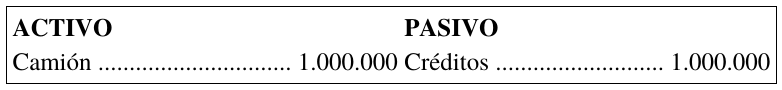
\includegraphics[width=0.80\linewidth]{figuras/fig_p120_45.png}
\end{center}

% ---- página 121 ----

Si nos fijamos en este Balance podemos observar uno de los \textbf{principios básicos de} \textbf{contabilidad}: El Activo siempre tiene que ser igual al Pasivo; en todo Balance de una empresa, obligatoriamente, el Activo tiene que coincidir con el Pasivo.

\textbf{Ejemplo 2:}

Vamos a suponer que en el caso anterior la empresa financia la compra del camión con \textbf{recursos} \textbf{propios }(capital). Su Balance Inicial sería:


\begin{center}
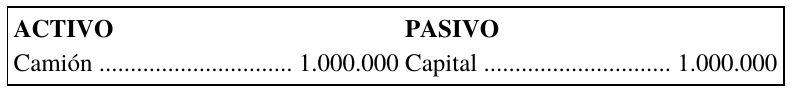
\includegraphics[width=0.81\linewidth]{figuras/fig_p121_46.png}
\end{center}

Comparando los dos ejemplos anteriores se puede ver como el Pasivo recoge el origen de los fondos de la empresa, sean propios (capital) o ajenos (créditos); por lo tanto, y como ya hemos comentado, es incorrecto considerar que el Pasivo representa lo que debe la empresa.


% ---- página 122 ----

\subsection*{ANEXO A}
\subsection*{LISTADO DE CÓDIGOS ARGENTINOS}
El texto completo de los códigos se puede obtener en Ministerio de Justicia y Derechos Humanos: www.biblioteca.jus.gov.ar

Código Aduanero (1982) Ley 22.415 y Decreto reglamentario 1001/82 Actualización por Ley 25.986 hasta el 12/2004

Código Aeronáutico (2007) Ley 17.285 y modificaciones hasta el 06/2007

Código Alimentario (2007) Ley 18.284 y Decreto reglamentario 2126/71 con modificaciones hasta el 06/2007

Código Civil (2006) Ley 340 con modificaciones hasta el 20/09/2006

Código de Comercio (1999) Ley 2.637 con modificaciones hasta el 29/12/1999

Código de Minería (1999) Ley 1.919 con modificaciones hasta el 29/12/1999

Código Penal (2007) Ley 11.179 con modificaciones hasta el 05/07/2007

Código Procesal Penal (2007) Ley 23.984 con modificaciones hasta el 04/06/2007

Código Procesal Civil y Comercial (2007) Ley 17.454 con modificaciones hasta el 21/03/2007

Código Electoral Nacional (2002) Ley 19.945 con modificaciones hasta el 10/2002

Código de Ética de la Función Pública (1999) Decreto 41/99 con modificaciones hasta el 10/11/1999

Código de Justicia Militar (1998) Ley 14.029 con modificaciones hasta el 17/04/1998


% ---- página 123 ----

\subsection*{CURSO: CONDUCCIÓN DE PERSONAL}
\subsection*{PROGRAMA}
\paragraph*{UNIDAD Nº 1: EL HOMBRE Y EL TRABAJO}
\subsubsection*{1.1. EL HOMBRE Y SU CONDUCTA.}
\subsubsection*{1.2. PSICOLOGÍA DEL TRABAJO.}
\subsubsection*{1.2.1. DESCRIPCIÓN PSICOLÓGICA DEL TRABAJO.}
\textbf{1.2.2. RELACIÓN ENTRE LA CONDUCTA DEL HOMBRE Y SU}

\subsubsection*{TRABAJO.}
\paragraph*{UNIDAD Nº 2: EL GRUPO HUMANO}
\subsubsection*{2.1. EL GRUPO HUMANO: CONCEPTO.}
\subsubsection*{2.1.1. CARACTERÍSTICAS DE LOS GRUPOS HUMANOS.}
\subsubsection*{2.1.2. CLASIFICACIÓN DE LOS GRUPOS.}
\subsubsection*{2.1.3. COMPONENTES DEL GRUPO.}
\subsubsection*{2.2. LIDERAZGO.}
\subsubsection*{2.2.1. FUNCIONES DEL LÍDER.}
\subsubsection*{2.2.2. TIPOS DE LÍDERES.}
\paragraph*{UNIDAD Nº 3: LA COMUNICACIÓN}
\subsubsection*{3.1. COMUNICACIÓN: CONCEPTO.}
\subsubsection*{3.2. ELEMENTOS DE LA COMUNICACIÓN.}
\subsubsection*{3.3. PATRONES DE LA COMUNICACIÓN: LIMITACIONES.}
\subsubsection*{3.4. COMUNICACIÓN DESCENDENTE Y ASCENDENTE.}
\subsubsection*{3.4.1. INFORMACIÓN SELECCIONADA.}
\subsubsection*{3.5. COMUNICACIONES LATERALES.}
\textbf{3.6. COMO ACTUAR FRENTE A LOS PROBLEMAS DE COMUNICACIÓN.}

\subsubsection*{3.7. COMUNICACIÓN. INFORMACIÓN.}
\paragraph*{UNIDAD Nº 4: SUPERVISIÓN}
\subsubsection*{4.1. ¿QUÉ ES UN SUPERVISOR?}

% ---- página 124 ----

\subsubsection*{4.1.2. ¿QUÉ ES SUPERVISIÓN?}
\textbf{4.1.3. LAS TRES MISIONES DEL SUPERVISOR EN RELACIONES}

\subsubsection*{HUMANAS.}
\subsection*{4.1.3.1. CORRECTO MANEJO DE LA AUTORIDAD.}
\textbf{4.1.3.2. CREAR UNA ADECUADA SITUACIÓN DE TRABAJO.}

\textbf{4.1.3.3. CONDUCIR EFICAZMENTE AL GRUPO DE TRABAJO.}

\subsubsection*{4.1.4. LOS MODELOS DE SUPERVISIÓN.}
\subsubsection*{4.1.5. EL MODELO AUTORITARIO.}
\subsection*{4.1.5.1. PRINCIPALES OBJECIONES AL MODELO}
\subsubsection*{AUTORITARIO.}
\subsubsection*{4.1.6. EL MODELO DE CONDUCCIÓN DEMAGÓGICO O}
\subsubsection*{PATERNALISTA.}
\subsubsection*{4.1.7. EL SUPERVISOR “LAISSES-FAIRE”.}
\subsubsection*{4.1.8. LA SUPERVISIÓN PARTICIPATIVA.}
\paragraph*{UNIDAD Nº 5: LOS PROCEDIMIENTOS BÁSICOS DE SUPERVISIÓN}
\subsubsection*{5.1. EL CICLO DE LA SUPERVISIÓN.}
\subsubsection*{5.2. EL CICLO SUPERVISOR.}
\subsubsection*{5.3. PRIMERA ETAPA: PLANEAMIENTO.}
\subsubsection*{5.4. SEGUNDA ETAPA: IMPLEMENTACIÓN.}
\subsubsection*{5.5. QUE SE DELEGA Y COMO.}
\subsubsection*{5.6. FACTORES DE MOTIVACIÓN.}
\subsubsection*{5.7. ETAPA CONTROL.}
\textbf{*************************************************************************}


% ---- página 125 ----

\subsection*{UNIDAD Nº 1. EL HOMBRE Y EL TRABAJO}
\subsubsection*{1.1. EL HOMBRE: Y SU CONDUCTA}
El siglo 19 fue el siglo del progreso material. En el siglo 20 y en el que ahora estamos viviendo, podríamos decir, que es el de la comprensión del ser humano, donde la Psicología Aplicada a la observación del Hombre tiene un papel principal. Esto nos guiara a ser testigos de cambios profundos en el funcionamiento de las Relaciones Humanas, que seguramente será más pronunciado y radical que el cambio material que comenzó hace más de 100 años y bajo cuyas consecuencias vivimos actualmente. Algunos cambios tienen un sentido positivo; otros, no.

Comprender los comportamientos del hombre y estudiar sus reacciones en una situación dada, partiendo desde la más extraña hasta lo que puede corresponder a lo más cotidiano, lleva un gran ejercicio de observación para poder entender sus propias necesidades y su modo de actuar, en consecuencia.

Cotidianamente intentamos hallar los motivos por los cuales alguien se conduce de un modo determinado; querríamos establecer los fundamentos de un comportamiento, conocer sus deseos y sentimientos. Esto lo podríamos averiguar conociendo los procesos psíquicos, de los cuales, algunos son conscientes, como por ejemplo la percepción, la atención y la memoria. Los actos que se realizan incluso por la voluntad y por los afectos, tanto los hostiles como los de amor son consecuencia de los procesos psíquicos.

El estudio de la conducta humana se establece con pilares como estos, que descubre el interior del ser humano. Son estudios subjetivos, como del interior, o proviniendo del interior del hombre y los expresa con su modo o su modalidad de actuar, es decir, viviendo de acuerdo a esa estructura formada.

Para comprender aun mejor estos alcances en el ser humano, se puede pensar que, tal como en el hombre se desarrolla un aparato físico, con un funcionamiento orgánico, con sistemas que controlan su equilibrio físico y su rendimiento, además este aparato  está en evolución permanente, y desarrollándose con leyes a las cuales tiene que adaptarse para vivir bien. Podríamos decir también que en él se forma un aparato que lo vamos a llamar mental o psíquico, que al igual que el físico, tiene un funcionamiento de acuerdo con los elementos que reúna, con sistemas que controlan todo el equilibrio para un mejor rendimiento; que también posee leyes, y que igualmente se desarrolla y evoluciona, al igual que el aparato físico, si todo está en


% ---- página 126 ----

orden, ya que cualquier alteración en cualquiera de los dos aparatos trae aparejado consecuencias que comúnmente conocemos como “enfermedad”.

Se realizaron experiencias en el siglo 19 (1870) que investigaron ciertos aspectos de los individuos, tal como la repetición de las aptitudes de un sujeto (ejemplo: La música, transmitida del abuelo al padre y luego al hijo) o en el carácter psíquico y se determino que algunos procesos psíquicos tienen un fundamento o una base orgánica que le da a esa función o actividad psíquica un determinado campo para establecerse. Este campo no podrá ser mayor que el que se forma y se dispone fisiológicamente, es decir, donde se apoyarían las funciones psíquicas en las que intervienen los procesos cerebrales (memoria, percepción, sensaciones) De aquí se podría deducir que el carácter lleva en su formación una cantidad de factores de tipo constitucional heredados pero a ellos se le sumaran después, los del ambiente en que vive y los de la educación que reciba: Todos ellos fundamentales para la vida posterior del hombre.

Aquí tiene importancia relevante el medio ambiente, constituido por la familia, por la escuela, por el club, por el lugar de trabajo, etc., en todo hombre existen disposiciones que solo se desarrollan en el caso de ser estimuladas por el ambiente que lo rodea. Por ejemplo: Un talento musical moderado puede quedar completamente sin desarrollar si no tiene ocasión para ello, pero en el caso que se lo fomentara podría ser un músico, y en este caso constituir esto una característica propia de su personalidad, sin que por ello sea precisamente un gran creador de música.

Se pueden sacar algunas conclusiones sobre estas investigaciones científicas con respecto al carácter y como se vuelca este en la vida de todos los días, en los diferentes ambientes en que circula un individuo y de acuerdo a ello puede decirse que al estimularse esas características e inquietudes, con visión de futuro y además tratando de evitar las perturbaciones del crecimiento y del equilibrio, se puede lograr un mejor desarrollo de la personalidad del sujeto que se está formando.

Se puede precisar el concepto de carácter y el de personalidad. \textbf{Por carácter se} \textbf{entiende la totalidad de las disposiciones psíquicas/intelectuales que tiene el} \textbf{hombre; como si dijéramos con lo que dispone, con lo que tiene o con lo que} \textbf{cuenta el ser humano. Por personalidad entendemos las disposiciones} \textbf{desarrolladas efectivamente, es decir las que se aplican en la práctica en un} \textbf{determinado momento de la vida de un hombre y con un ambiente determinado.} \textbf{Esto sería como si detuviéramos a la persona en un momento de su desarrollo} \textbf{para ver que características tiene, es así porque la personalidad está en} \textbf{constante expresión y lo que hasta hoy no se manifestó puede aparecer} \textbf{mañana, como un elemento nuevo de su evolución.}


% ---- página 127 ----

Un individuo nacido en un lugar determinado, con características y formación determinadas, tendrá una personalidad determinada por ese ambiente y por la educación recibida, y si a este individuo se lo trasladara a otro ambiente, inexorablemente la personalidad se modificaría, aunque lo heredado o lo constitucional sea igual. ¿Por qué?. Porque en cada uno de ellos se fomentarían determinadas características; además los hogares seguramente estarán conformados en forma diferente y esto traerá otros modos de vida diferentes, no pudiendo ser más que de una sola forma: Al modificarse alguno de los tres factores: Ambiente, constitucional heredado, y educación, se modifica el resultado final que es la formación de la personalidad misma. Otro tanto sucede en el transcurso de la vida, el tiempo es también un factor importante que nos abre el panorama para pensar que la historia de una persona se va haciendo de esta forma. Todo este proceso, si es cumplido en forma favorable, dará como resultado la evolución del hombre, que será distinta entre uno y otro, pero a la vez igual, porque se da en todos ellos; todo apunta a la unificación y formación como sujeto.

\textbf{Desde que nace, el hombre se conduce solo, no deja de conducirse. Esta} \textbf{expresión se la tiene que tomar al pie de la letra; no está conducido desde} \textbf{afuera de él cómo se conduce una máquina; sino que él mismo es el propio} \textbf{conductor. ¿Por qué es así?, porque para poder seguir persistiendo o viviendo} \textbf{al igual que se alimenta para vivir, también necesita comportarse o conducirse} \textbf{de determinada manera para asegurar su vida. Entonces esa conducta que toma} \textbf{la definiremos como: Las acciones que realiza con relación a la información} \textbf{recibida o a lo requerido por el medio ambiente o por el interior de él, que} \textbf{provoca en el individuo la tendencia hacia algo, a una reacción. Por eso la} \textbf{personalidad, se expresa por medio de conductas, pero también es cierto que} \textbf{la conducta muestra una personalidad, es decir, que conducta y personalidad} \textbf{son dos aspectos que se complementan en un mismo individuo y hacen a su} \textbf{historia personal.}

La conducta sufre transformaciones con el curso del tiempo, que generalmente son intensas y fundamentales.

\textbf{Conducta y personalidad.}

\textbf{Lo que debemos subrayar es que son dos elementos que se complementan con el} \textbf{tiempo en forma constante y dinámica, integrando continuamente nuevas} \textbf{posibilidades y eliminando otras, teniendo en cuenta que están conformadas por} \textbf{elementos adquiridos y por otros ya dados en forma hereditaria como} \textbf{predisposiciones.}


% ---- página 128 ----

\subsubsection*{1.2. PSICOLOGÍA DEL TRABAJO}
El trabajo es una situación humana. La psicología del trabajo estudia la conducta del hombre en esa situación.

Trataremos de poner en claro, en que consiste el trabajo desde el punto de vista psicológico.

\subsubsection*{1.2.1. DESCRIPCIÓN PSICOLÓGICA DEL TRABAJO}
El trabajo tiene en nuestra cultura, una concentración y un reconocimiento social. Lo hace un hombre con los otros hombres, bien en contacto directo con ellos, o bien, a través de usos técnicos y/o por medio del trato social. El trabajo es una situación social en la que el hombre, de modo más o menos voluntario u obligatorio, produce algún bien estimado por la sociedad.

\textbf{El trabajo es un tipo de conducta del hombre en cierto tipo de situación} \textbf{humana. ¿Cuáles son las notas distintivas que hacen al trabajo en sí?. Estas} \textbf{serian, por ejemplo, que trabajar es, desde luego, producir algo. Además} \textbf{posee el trabajo, a diferencia del juego y la diversión, un matiz obligatorio; a} \textbf{su vez ordena la producción de algo, que va a satisfacer o pretende satisfacer} \textbf{alguna necesidad, consecuencia o demanda del hombre y estimado por la} \textbf{sociedad.}

La psicología del trabajo estudia el comportamiento del hombre en esa situación. Su fin principal es conocer ese comportamiento, sus características, su evolución y sus estructuras. En ese sentido la psicología del trabajo es una ciencia teórica. Es esa parte de la psicología diferencial que estudia lo que distingue a cada situación y a cada tipo de hombre de los demás hombres y de las demás situaciones. \textbf{Pero el} \textbf{estudio de la conducta humana en el trabajo solo puede hacerse en la situación} \textbf{concreta, es decir en el taller, en la fábrica, en el comercio, en la} \textbf{oficina...observando el trabajo, describiéndolo tal como se realiza, inventando} \textbf{hipótesis explicativas de lo observado y lo descrito, modificando el trabajo} \textbf{mismo para confrontar esas hipótesis. Incluso cuando podemos estudiar en el} \textbf{laboratorio un problema laboral, los resultados obtenidos deben ser} \textbf{confrontados en el ámbito social y en el ámbito efectivo del trabajo}. La psicología del trabajo, tiene como objetivo conseguir que el trabajo sea eficaz.


% ---- página 129 ----

\textbf{1.2.2. RELACIÓN ENTRE LA CONDUCTA DEL HOMBRE Y SU TRABAJO}

\textbf{¿EN QUÉ CONSISTE LA CONDUCTA HUMANA EN EL TRABAJO? ¿CÓMO}

\subsubsection*{INFLUIR EN ELLA PARA AUMENTAR SU EFICACIA?}
Tales son los temas centrales de la psicología del trabajo como teoría y como aplicación. Examinaremos con más detalles la situación en que esta conducta humana se realiza. Comprende tres aspectos principales:

a) EL PERSONAL: Hay siempre una persona que trabaja.

b) EL PRODUCTIVO: Siempre se hace algo.

c) EL SOCIAL: Siempre se realiza en un determinado ámbito social.

En primer lugar el trabajo es una actividad personal. No solo es un proceso técnico o un conjunto de operaciones y movimientos, o un gasto de energía mensurable, sino que el trabajo es, ante todo una actividad personal.

Esto quiere decir que es un HOMBRE el que trabaja, un hombre como totalidad, no como una parte aislada de él; no sus músculos o sus aptitudes, o una cierta habilidad. Es un hombre que en el trabajo y mediante el trabajo vive, hace su vida y al mismo tiempo influye en la vida de los demás. No solamente el trabajo depende de la personalidad del trabajador, sino que recíprocamente, la personalidad del trabajador depende del trabajo. Se trabaja según se es, pero, a la inversa se va siendo según se trabaja.

El hombre es una personalidad que, con la naturaleza que le es dada, va haciendo su personalidad, su manera peculiar de comportarse, de creer, de pensar, de querer y de sentir, a medida que va haciendo sus diversos quehaceres en el trato con la realidad. El trabajo es una forma de trato con la realidad, una manera de hacerse a sí mismo y de hacer a los demás. El hombre llega al trabajo con personalidad propia: Como trabaje, dependerá por un lado de como sea, y por otro, de cómo la nueva situación influye en su modo de ser.

a) Un trabajo eficaz será aquel que ofrezca al trabajador la oportunidad de expresar su personalidad y la estimule para desarrollarla y enriquecerla.

b) En segundo lugar, el trabajo es una actividad productiva. A través de la expresión de su personalidad y al mismo tiempo en que su actividad la va modificando el hombre produce algo. Un trabajo eficaz será aquel que favorezca


% ---- página 130 ----

mediante la expresión y el desarrollo de la personalidad del trabajador una producción elevada.

c) En tercer lugar, finalmente, el trabajo es una forma de convivencia. El trabajo no es solamente una situación personal y productiva, sino interpersonal y social. Se trabaja con otros. De su personalidad, en las relaciones humanas que entre los que forman la empresa se establezcan, del sentido que tenga el trabajo en la sociedad en que la empresa se integra, en la estructura general de esa sociedad, en sus aspectos más diversos: económicos, sociales, morales, etc.

No solo los otros influyen en el trabajo; también influyen en el trabajador. Como en las demás situaciones, el hombre, al expresarse y modificarse, contribuye a la expresión y modificación de los demás. Al menos en nuestra cultura, el trabajo es, con la familia y con la escuela, una de las formas de convivencia más extendida y más estable. La estructura humana del trabajador, es al tiempo uno de los exponentes más reveladores de la estructura de la sociedad toda, y una de las situaciones que más influyen en la manera de incorporarse el individuo a la sociedad.

Trabajo eficaz, será: “Aquella situación humana en la que el trabajador consiga una alta producción, a través de la expresión y el desarrollo de su personalidad, en un ambiente técnico e interpersonal que favorezca su sana incorporación a un grupo y a una sociedad”.

Estos tres fines del trabajo: Desarrollo personal, incorporación social y alta producción, constituyen un delicado equilibrio, porque muchas veces pueden entrar en conflicto incluso, cualquier mejora del trabajo, al modificarlo a la nueva situación, plantea nuevos problemas. Y los nuevos problemas requieren soluciones que deben estar encuadradas dentro de las tres dimensiones en que hemos considerado el trabajo.

*************************************************************************


% ---- página 131 ----

\subsection*{UNIDAD 2. EL GRUPO HUMANO}
\subsubsection*{2.1. EL GRUPO HUMANO: CONCEPTO}
\textbf{“}Dos o más personas entre las que existe una pauta establecida de interacción psicológica, se reconoce como una entidad por sus propios miembros y, por lo general, por los demás, en razón del tipo en particular de conducta colectiva que representa”.

Es decir, para que exista grupo, debe haber por lo menos dos o más personas, que interaccionan o interactúan entre sí, que se comunican, que trabajan juntos, que juegan, que estudian, etc. En otras palabras las relaciones son reciprocas.

Otra cualidad, es el sentido o la conciencia “del nosotros” que experimentan los miembros, complementados por el reconocimiento como grupo que le otorgan los demás.

El grupo es también un sistema porque en él los elementos de la conducta tienen una dependencia mutua. Es decir que podemos hablar de un sistema interno y uno externo, ambos forman el sistema social. Entendiéndose por sistema interno o endogrupo el grupo propio, aquel que privilegiamos con respecto a otros y por consiguiente el sistema externo o exogrupo será el que está formado por los “otros”.

\subsubsection*{2.1.1. CARACTERÍSTICAS DE LOS GRUPOS HUMANOS}
La existencia de grupos humanos deviene de la condición social del hombre. Es prácticamente inconcebible imaginar alguna persona que se halla psicológica y afectivamente aislada de los demás. La actividad de los hombres tiene siempre lugar dentro de grupos o de asociaciones. Es más, las personas quieren ser algo más que simples miembros de un grupo, quieren pertenecer a él.

Avanzando en nuestra línea de análisis observamos las siguientes características:

- Interacciones entre los componentes.

- Objetivos compartidos.


% ---- página 132 ----

- Un creciente compromiso de cada integrante respecto del resto de los componentes.

- Un cierto grado de modificación de los comportamientos individuales en virtud de las exigencias manifiestas y latentes impuestas por la pertenencia al agrupamiento.

El grupo brinda a sus miembros una serie de elementos, de pautas, y de guías, que le ayudan en diversas circunstancias de la vida. ¿Qué posibilidades brindan un grupo a sus miembros?

- Reconocimiento afectivo: Sucede cuando se ha llegado a una condición reciproca de amistad, entendiéndose por amistad la adaptación emocional del hombre al medio, que podría extenderse desde la camaradería o el compañerismo hasta una amistad profunda.

- Guía de comportamientos: Muchas veces el ser humano se encuentra en situaciones sociales nuevas o inéditas, que conducen a una sensación de inseguridad, sobre la forma en que debe comportarse. El grupo llena esa necesidad importante de proporcionar a todos sus miembros una especie de “guía de comportamiento aceptable”, no sobre la base de cualquier política o de norma escrita, sino en razón de lo que es realmente aceptable por el grupo.

- Ayuda a resolver problemas: El grupo le permite a sus miembros compartir sus problemas brindándole de esta manera comprensión, apoyo emocional, u orientándolo en la búsqueda de soluciones.

\textbf{Solidaridad entre los miembros del grupo}

El grupo desarrolla actividades de solidaridad que se expresan a veces en la resistencia a aceptar cambios en las modalidades de trabajo, o acordando entre todos seguir una determinada pauta con respecto a personas, a temas, a tareas, etc.

\subsubsection*{2.1.2. CLASIFICACIÓN DE GRUPOS}

% ---- página 133 ----

Observando la pluralidad de grupos sociales distinguimos básicamente dos tipos, unos más “cerrados” y en general muy intensos, y otros más flexibles y con mayor número de componentes. Los primeros se denominan grupos primarios, y los segundos grupos secundarios.

Señalaremos sintéticamente las características de cada uno de ellos:

\textbf{1º) GRUPO PRIMARIO. }(Ej.: La familia, el grupo de trabajo, el grupo de amigos íntimos que “paran” en el mismo bar)

Es un grupo pequeño, donde existe una total interacción entre sus miembros (relación “cara a cara”), existiendo lazos afectivos, y persiguiendo un objetivo común.

En forma sintética, podríamos señalar las siguientes características:

-  está integrado por un numero restringido de personas, lo cual permite la relación a nivel individual entre todos ellos.

- Prosecución en común y de manera activa de los mismos objetivos que están dotados de una gran permanencia asumidos como objetivos del grupo, que responden a diferentes intereses de los miembros y por lo tanto, valorizados por ellos.

- Relaciones afectivas que pueden llegar a ser muy intensas entre los miembros (simpatías o antipatías), que tienden a favorecer la unión del grupo, pero que en momentos difíciles, pueden llevar a la constitución de sub-grupos o camarillas.

- Diferenciación de roles entre los miembros; constitución de normas, de creencias, de signos e incluso, de ritos propios del lenguaje grupal.

\textbf{2º) GRUPO SECUNDARIO (U ORGANIZACIÓN)}

Es aquel que funciona regido por instituciones. Una empresa industrial, un hospital, una escuela, un partido político, son instituciones.

Contrariamente a lo que sucede en el grupo primario, en este otro tipo de grupo, las relaciones tienden a ser frías, impersonales, contractuales y formales; las comunicaciones por escrito llegan a adquirir mayor importancia que las comunicaciones orales.

\subsubsection*{OTRAS CALIFICACIONES}

% ---- página 134 ----

- \textbf{Grupos de pertenencia}: Son aquellos a los cuales un sujeto pertenece en forma simultánea. Ejemplo: El grupo de familia, el grupo de trabajo, el grupo de asociados a una institución, el grupo de afiliados a un gremio o a un partido político.

Característica principal es, que todos los miembros, en grado variable, se sienten pertenecientes al grupo o grupos en cuestión.

- \textbf{Grupo de referencia: }Es el grupo cuyos valores, aptitudes u opiniones sirven de referencia. Habitualmente, los grupos de pertenencia son también grupos de referencia, pero existe una variedad de grupos a los cuales no pertenecemos y cuyos valores o actitudes nos sirven de referencia. Por ejemplo las opiniones de conocidos escritores o intelectuales que opinan sobre temas ajenos a su quehacer literario, como ser política o problemas sociales, y que sirven como marco de referencia a vastos sectores de la comunidad. Otro tanto ocurre con instituciones como la iglesia (en cuanto no somos miembros activos de ella), las asociaciones científicas, las cámaras de producción o de comercialización. Los medios masivos de comunicación hace uso frecuente de figuras populares, que en algunos aspectos obran como “modelos” en los cambios de modas o difusión de “clisés”, de esquemas verbales, de modismos, etc.

\subsubsection*{2.1.3. COMPONENTES DEL GRUPO}
Todos los estudiosos del tema, concuerdan básicamente, en distinguir los siguientes componentes:

1º) Las personas (que son las que cumplen roles)

2º) Estructura del grupo (es la red de afinidades y de antipatías entre las personas)

3º) Organización interior: Normas, creencias, valores, reglas.

Haremos una descripción de estos tres componentes.

\textbf{1º) Personas}

Se ha señalado que todo grupo  está compuesto por personas. A pesar de que todas esas personas tengan ciertas características comunes, (ej.: Sexo, edad, nivel de estudios, procedencia social, participación en la tarea común), debe tenerse en


% ---- página 135 ----

cuenta, que todas ellas, son distintas. Para decirlo de otra manera, cada una tiene su personalidad. Merece tenerse en cuenta que esta heterogeneidad tiene gran importancia para la eficacia del grupo, porque, aunque es generadora de tensiones, resulta ser al mismo tiempo el motor de la participación del grupo y fuente de su creatividad.

Entre los aspectos de esta heterogeneidad, podemos distinguir:

- Por una parte, funciones, comportamientos, tareas habituales que caracterizan a cada uno de los participantes; esas conductas son deseadas, alentadas, aceptadas o solamente toleradas por el grupo. De todas maneras, están en relación con la posición que el participante (o miembro) ocupa en el conjunto que constituye el grupo.

Nos referimos a ellas con el término genérico de ROLES.

- Por otra parte, todos los miembros manifiestan con respecto a las personas, las cosas y las situaciones, una disposición durable, que constituye su repuesta a los mismos. Estas disposiciones (o actitudes), pueden ser inducidas por la vida en grupo, pero también pueden relacionarse con los roles.

Dado lo expresado en los dos puntos anteriores, resulta conveniente hacer alguna alusión a lo que entendemos por ROLES.

\textbf{Definición}

Un grupo no escapa al fenómeno de la división del trabajo, sobre todo, si las situaciones a las cuales se enfrenta, tienen aspectos relativamente complejos. Por lo tanto, los individuos tratan de especializarse de acuerdo con sus capacidades y sus motivaciones propias, y de acuerdo también a la reacción del grupo frente a sus intenciones.

El comportamiento esperado por parte de un individuo definido de acuerdo con sus “especialidades” constituye el conjunto de “ROLES”.

Esto puede explicarse mejor, siguiendo el siguiente razonamiento. Todo hombre ocupa una posición en el sistema social. A esa posición, se le da el nombre de STATUS. Por ejemplo, un individuo puede tener el status de ciudadano, de supervisor en la empresa, de padre de familia, de ingeniero, de católico. El ROL es el conjunto de conductas consideradas normales para el poseedor de un “STATUS”.

Dentro de un grupo de trabajo, los diferentes miembros que lo componen cumplen roles distintos.


% ---- página 136 ----

Debe señalarse que, en determinados individuos, puede surgir un conflicto entre roles que corresponden a status diferentes; por ejemplo en el momento de tomar una decisión, un supervisor puede sentirse íntimamente dividido entre el rol que debe asumir conforme al status en la empresa, y su rol en cuanto miembro de un grupo de amigos íntimos.

Conflictos entre roles de este tipo son frecuentes en la vida corriente de trabajo. La lealtad respecto del grupo puede enfrentarse con la lealtad respecto de la organización.

\textbf{2º) Estructura del grupo}

Una vez que el grupo ha quedado bien establecido (por ejemplo un grupo de trabajo) puede cumplir con sus fines, como así también, mantenerse a través del tiempo.

¿Cómo logra estos propósitos?. Los consigue:

1º) Creando un conjunto de características que determinan las reacciones entre uno y otro de sus miembros.

2º) Determinando las relaciones entre los miembros y el supervisor.

3º) Mediante las normas de conducta que están aprobadas y que el grupo hace cumplir, aplicando un sistema propio de retribuciones y de castigos.

4º) Mediante el sistema de comunicaciones internas y externas.

Todos estos aspectos de la vida del grupo forman un verdadero sistema, porque:

1- Están todos ellos relacionados entre sí.

2- Todo cambio en uno de ellos sufre efectos inmediatos en los demás.

3- Los miembros se resisten a todo cambio en cualquiera de los puntos del sistema interrelacionado.

\textbf{3º) ¿Cuáles son las características que deciden la organización interior del} \textbf{grupo?}

Tales son:

\textbf{a) Jefatura. }(Este aspecto se dará en el punto destinado a liderazgo) Podemos decir, en forma muy resumida, que el jefe lleva a cabo funciones vitales que contribuyen a una mayor capacidad del grupo. Así:

- Inicia la acción.


% ---- página 137 ----

- Facilita el consenso.

- Perfecciona el contacto o el enlace con el mundo exterior, ya sea con los mandos, con otros grupos de trabajo, o con el sindicato.

\textbf{b) Reglas del grupo. }El afán de conformarse a las reglas del grupo impregna la mayor parte de la vida social. Esta necesidad se hace muy evidente durante la adolescencia. En los grupos de trabajo también son frecuentes, y pueden tener por finalidad:

- Hacer más agradable la convivencia.

- Hacer que el trabajo sea más fácil.

- Elevar o mantener el prestigio del grupo a través de la calidad de su trabajo.

- Protegerse contra los peligros exteriores, reales o imaginarios, y en particular de los procedimientos de los mandos.

\textbf{c) Normas del grupo. }Las personas que trabajan en estrecho contacto y forman un grupo, elaboran puntos de vista comunes que se espera, serán compartidos por todos. Ej.: Tenemos esta norma: “en nuestro sector, hay que ser muy buen operario para desempeñarse bien”.

Entra entonces en acción el fenómeno de la sugestión, mediante el cual en forma no deliberada, el individuo va aceptando los criterios del grupo.

\textbf{d) Presiones para amoldar a los miembros. }Las personas muestran interés por amoldarse a las reglas del grupo, no solo porque desde que son miembros, adoptan sus puntos de vista, sino también porque el grupo cuenta con medios efectivos para castigar a los que insisten en hacer las cosas a su manera. Por ejemplo se apela a la marginación, o se interrumpe la información y la comunicación, no se le advierte sobre riesgos o sobre errores que pudiera cometer.

\textbf{e) Sistemas de rango. }En el conjunto de personas que forman un grupo, aparecen sutiles diferencias de rango (lugar en una escala de prestigio), que puede estar relacionado con la posesión de títulos, o bien, de monto del sueldo, de jerarquía, de horario de trabajo, de asignación de determinadas tareas, etc.

\textbf{TRABAJO PRÁCTICO. Grupo Humano}

-Defina las características, clasifique y distinga los componentes de “su” grupo humano, de acuerdo a lo visto en clase (apunte)


% ---- página 138 ----

\subsubsection*{2.2. EL LIDERAZGO}
\textbf{LÍDER. }La definición de “líder” resulta algo complicada, ya que el vocablo, procedente del idioma inglés, ha sido incorporado a nuestro idioma, con distintas acepciones o variaciones de interpretación y de complejidad. En el diccionario de sociología, leemos:

1º) En el sentido más amplio, “el que dirige, por ser el iniciador de una conducta social; por dirigir, organizar o regular los esfuerzos de otros, o por prestigio, poder o posición; el verdadero impulsor de la conducta social”.

2º) En sentido estricto, “la persona que dirige, por medios persuasivos y en mérito a la aceptación voluntaria de sus seguidores”.

De estas definiciones, podemos pasar a la de liderazgo:

a) Proceso-situación en que una persona (o varias) en mérito a su capacidad real o supuesta para resolver los problemas cotidianos en la vida o en grupo, encuentra seguidores que se hallan bajo su influjo.

b) Acto de organizar y dirigir los intereses y las actividades de un grupo de personas, unidas para un proyecto o una empresa que fomenta su cooperación por el hecho de lograr que todos ellos aprueben, más o menos voluntariamente, determinados fines y métodos.

Analizando las definiciones expuestas, surgen las siguientes apreciaciones:

1. No existe ningún grupo sin líder. Podría darse la situación que existan varios. En este caso, la situación y la diversidad de los problemas, determinaran el surgimiento de uno de ellos.

2. En los grupos, el líder no es impuesto, sino aceptado por distintos motivos por los miembros del grupo. Al margen de esta aceptación, la forma de ejercer el liderazgo puede ser muy variada.

\subsubsection*{2.2.1. FUNCIONES DEL LÍDER}
Las funciones principales del líder son las siguientes:

a) Mantener la cohesión del grupo.


% ---- página 139 ----

b) Asumir la responsabilidad y la circunstancia de dirigir los esfuerzos de los demás miembros, para lograr el objetivo deseado.

c) Orientar al grupo acerca de los fines que le caben por su actividad o por su modalidad.

d) Encontrar y elaborar las soluciones más convenientes.

e) Servir como intermediarios, como representantes o como “modelos” entre las otras personas o grupos externos, con los cuales el grupo mantiene cualquier tipo de relación (tanto positiva como negativa) y asumir los riesgos que implican estas decisiones.

Delimitadas así las funciones del líder, corresponde aclarar que, en este curso, se ha separado y distinguido deliberadamente, esas dos funciones fundamentales que son el liderazgo y la jefatura, ya que ambas, si bien pueden coincidir en una persona, pueden darse en forma separada e independiente dentro de un mismo grupo, aunque el ideal lo constituye el jefe (supervisor) que adquiere cualidades del líder.

¿Qué factores determinan que una o varias personas asuman el liderazgo? Algunas de las respuestas que se han brindado, están entre las siguientes:

a) Cualidades personales: (Aspecto físico, valor, simpatía, inteligencia) b) Prestigio otorgado por conocimientos sumamente valorados dentro del grupo. c) Combinación de ambos tipos de cualidades.

En una de las más conocidas investigaciones realizadas en el área laboral, se describió de esta manera a un líder: “Era el que más se acercaba al ideal del grupo. Se hallaba en buenos términos con todos los integrantes del salón de trabajo y siempre estaba dispuesto a intervenir en un juego o en una conversación. Todos los miembros del lugar de trabajo contaban con una invitación a su casa. Los operarios demostraban el afecto que le tenían, ayudándolo más que a ningún otro obrero de la sala, aunque él no siempre devolvía el favor. Era un conversador infatigable. Hallándose o no trabajando, mantenía un continuo torrente de charla. Pocas veces perdía una discusión, no importando el tema que se tratara. Su superioridad se manifestaba no solamente en ello, sino también en la forma en que aconsejaba o amonestaba a los demás compañeros”.

Esta descripción nos coloca frente a un tipo especial de líder. Se destaca su inteligencia lógica y verbal, su alta capacidad técnica, su “carisma” evidenciado en el afecto que inspiraba, sus conocimientos generales (cultura) y hasta su ascendiente sobre los demás compañeros.


% ---- página 140 ----

Pero esto no significa que TODOS los líderes sean así. En verdad, no existe todavía una respuesta absolutamente satisfactoria, acerca de las condiciones que debiera reunir necesariamente una persona para llegar a convertirse en un líder.

\subsubsection*{2.2.2. TIPOS DE LÍDERES}
Se han ensayado distintas tipologías; lamentablemente no contamos con un acuerdo más o menos amplio. No obstante, seguiremos algunas de las usadas con mayor frecuencia:

a) Líder autocrático.

b) Líder democrático.

c) Laissez-faire (paternalista)

Las principales características, son las señaladas en el cuadro que sigue:

\subsection*{Comportamientos del monitor}
\subsection*{en las experiencias de Lippit y White.}

\begin{center}
\small
\begin{tabular}{|p{\dimexpr0.245\linewidth-2\tabcolsep\relax}|p{\dimexpr0.245\linewidth-2\tabcolsep\relax}|p{\dimexpr0.245\linewidth-2\tabcolsep\relax}|p{\dimexpr0.245\linewidth-2\tabcolsep\relax}|}
\hline
Comportamiento del monitor & \multicolumn{3}{|p{\dimexpr0.735\linewidth-2\tabcolsep\relax}|}{Características de los grupos} \\ \hline
 & Autocrático & Democrático & Laissez-faire o paternalista \\ \hline
Toma de decisión & Por el jefe únicamente & En común con el jefe (discusión) & Indeterminación; débil participación del jefe \\ \hline
Determinación de las actividades y de las técnicas & Dadas por el jefe & Objetivos generales trazados por el jefe indicando las alternativas & Ninguna ayuda del jefe, quien proporciona (a pedido) material o información \\ \hline
División de la tarea & Por el jefe & División espontánea del trabajo & Ninguna intervención del jefe \\ \hline
\end{tabular}
\end{center}

% ---- página 141 ----

\begin{center}
\small
\begin{tabular}{|p{\dimexpr0.245\linewidth-2\tabcolsep\relax}|p{\dimexpr0.245\linewidth-2\tabcolsep\relax}|p{\dimexpr0.245\linewidth-2\tabcolsep\relax}|p{\dimexpr0.245\linewidth-2\tabcolsep\relax}|}
\hline
Composición de los grupos de trabajo & Por el jefe & Libre elección de cada uno & Ninguna intervención \\ \hline
Apreciaciones & De tipo “personal” (aliento, critica) & De tipo objetivo & Ninguna, no hay comentarios \\ \hline
Participación en las actividades & Ninguna participación & Participa & Ninguna participación \\ \hline
\end{tabular}
\end{center}

\paragraph*{a) El líder autocrático}
Es el que se arroga la conducción del grupo, toma decisiones sin efectuar consultas, es individualista y autoritario. En los grupos con este tipo de líder, los actos de conducta democráticos están muy limitados. Hay grandes diferencias de prestigio entre sus miembros y la comunicación tiene lugar en un solo sentido: De los conductores a los partidarios. Las ideas se aceptan sobre la base de su origen, no de su valor intrínseco. Algunas de las consecuencias observadas son:

\begin{itemize}
  \item El líder concentra el mayor número de “elecciones” y de “rechazos”.
  \item El grupo adopta una estructura que descansa en el líder.
  \item En las conversaciones y las actitudes se percibe: -Un máximo de hostilidad frente al jefe y un mínimo de sociabilidad entre los miembros.
\end{itemize}
-Un máximo de competencia y de agresividad entre los miembros.

-Un mínimo de “conciencia” puesta en el cumplimiento de la tarea (el rendimiento disminuye en ausencia del líder)

-Un máximo de dificultad para reemplazar al jefe en caso de alejamiento de éste.

Debe agregarse, sin embargo, que existen dos modos de reacción entre los grupos de autoridad autocrática: Unos son abiertamente agresivos mientras que otros, son totalmente apáticos.

\textbf{b) Líder democrático} Actúa sobre la base del consenso del grupo, logrando la participación de sus miembros, conforme con sus aptitudes.

Se ha observado que en estos grupos hay más elecciones intercambiadas entre los miembros (y no concentradas en el líder), la estructura de grupo es como una “red”,


% ---- página 142 ----

ya que se dan considerables afinidades entre sus miembros. Otro detalle importante: Los miembros demuestran una mayor madurez.

\textbf{c) El líder “Laissez-faire”}

Se presenta muchas veces al no darse una organización. El liderazgo tiende a ser pasivo e incluso, se abandona la responsabilidad y la acción en manos del grupo, pero sin dejar sugerencias. Se presenta también una gran ineptitud para realizar cualquier propósito. Estos grupos de trabajo se caracterizan por su falta de productividad.

*************************************************************************


% ---- página 143 ----

\subsection*{UNIDAD 3. LA COMUNICACIÓN}
\subsubsection*{3.1. COMUNICACIÓN}
Toda actividad social postula intercambio de informaciones, ya sea entre los miembros de un mismo grupo, o bien, entre miembros de grupos diferentes. “Una sociedad está constituida por individuos y por grupos que se comunican entre sí”, ha afirmado un conocido investigador. Además, es necesario que los grupos se organicen, en primer lugar, para recoger informaciones útiles y eficaces, y en segundo término, para que esas informaciones se distribuyan convenientemente entre todos los que deberán utilizarlas, especialmente aquellos que tendrán que tratarlas para organizar decisiones validas.

La forma en que se efectúan esos intercambios condiciona las relaciones entre los miembros.

Conocemos la ambigüedad de la palabra “entender” y “comprender” y recordaremos a este propósito la afirmación de Saint-Exupery: “El lenguaje es fuente de equívocos”. Esta afirmación resulta valida cada día. Vemos aparecer conjuntos humanos cada vez más complejos y más diferenciados, mientras que en las organizaciones de toda naturaleza surgen nuevos obstáculos a la comunicación, tales como: La sobre dimensión; las divisiones en compartimentos aislados; la tensión entre concentración económica y administrativa y la descentralización geográfica, etc.

\textbf{Definiciones y distinciones}

- La información es a la vez una operación (la acción de informar) y un contenido (lo que se informa) que tienden a una reducción del desorden.

- La comunicación es el conjunto de procesos físicos y psicológicos mediante los cuales se efectúa la operación de relacionar a una (o varias) persona – el emisor

– con otra (u otras) persona/s – el receptor – con el fin de alcanzar determinados objetivos.

\subsubsection*{3.2. LOS ELEMENTOS}

% ---- página 144 ----

Quienes se ponen en contacto son: Un “locutor” y un “alocutorio” (o receptor); en otras palabras, dos o varias personalidades comprometidas en una situación común y que luchan con las significaciones. A este esquema podemos suponerle los campos de conciencia del emisor y del receptor.

Los elementos esenciales son:

- \textbf{Personalidades: }Los individuos que se comunican están caracterizados por: Su historia personal, sus sistemas de motivaciones, sus estados afectivos, su nivel intelectual y cultural, un marco de referencia, un status social y los roles psicosociales. Estos diversos factores influyen en la emisión y la recepción de los mensajes.

- \textbf{Situación común: }La comunicación posibilita la acción sobre los demás dentro de una situación definida. Es un medio para hacer cambiar esa situación.

Hay que tener en cuenta, igualmente, los objetivos de la comunicación; por ejemplo: Informar, convenir, convencer, modificar una opinión, hacer actuar, callar, expresar sentimientos, instruir, inducir sentimientos, etc.

Los objetivos influyen sobre el contenido y el estilo de las comunicaciones.

Finalmente, la naturaleza de la situación puede ser tal que suscite en los interlocutores una necesidad más o menos intensa de comunicación, y a veces, la negativa de uno de ellos en entrar en comunicación.

- \textbf{Significación: }Los hombres no solamente se comunican determinada cantidad de información, sino que también intercambian significaciones. “Sin ellas, los ademanes y palabras de los hombres formarían un inmenso bosque, en el que cada árbol crecería para sí y extendería sus ramas sin tener en cuenta a los otros árboles” (Bogardus)

\subsubsection*{3.3. PATRONES DE COMUNICACIÓN. LIMITACIONES}
La relación entre supervisor y subordinados es uno de los elementos básicos de la organización. La idea de mando, en virtud de la cual una persona dirige a otras, es fundamental para llevar a cabo sistemáticamente la división de deberes y las


% ---- página 145 ----

responsabilidades. También tienen su importancia, las distintas misiones y las expectativas de dirigentes y de dirigidos. El jefe tiene la responsabilidad de conseguir que un trabajo se lleve a cabo dentro de las normas impuestas por sí mismo o por la organización. Como jefe tiene que hacer todo, influyendo sobre sus subordinados. Debe dirigirlos, juzgarlos, motivarlos, etc. Y a menos que sea eficaz, no podrá conseguir que se ejecute el trabajo. Por otra parte, el jefe espera de los subordinados:

1º) Que acepten sus derechos a dirigir, a dar órdenes y a juzgar.

2º) Que obedezcan sus órdenes.

Los subordinados, a su vez, tienen ciertas responsabilidades y expectativas. Tienen la responsabilidad de ejecutar las órdenes. Y esperan que estas sean:

1º- Comprensibles.

2º- Factibles.

3º- Razonables.

4º- Relacionadas con su trabajo y con la situación laboral.

La máxima preocupación de un jefe consiste precisamente en lograr que la gente realice sus COMETIDOS. Si examinamos cualquier situación de trabajo comprobaremos que, en general, existe una gran aceptación de las órdenes y una considerable obediencia respecto a las normas y las directivas impuestas por la dirección y reforzadas por los mandos medios. Es la cadena de mando: Podemos observarlo en los eslabones de la relación entre el personal de base y la alta dirección. Todas las personas, dentro de la estructura completa forman una pirámide con un jefe superior en la cúspide, y cada rango de jefes menores, aumentando el número conforme desciende hasta la base de la estructura inspectora, donde está el grupo mayor y quizás el más incomprendido: El de los supervisores o mandos de primera línea. Lo mismo que las líneas de autoridad que convergen hacia el vértice de la estructura, las líneas de interés y de atención convergen también.

Ahora bien: Uno de los conceptos fundamentales de la ORGANIZACIÓN FORMAL, es el ir agrupando las responsabilidades en menor número de individuos a medida que se asciende desde la base a la cima de la organización. Cada jefe tiene la responsabilidad y el mando de varios subordinados, pero solo depende, a su vez, de un jefe (unidad de mando) de suerte que ante el hombre que está en el nivel


% ---- página 146 ----

superior solo son responsables unos pocos, que se encargan de transmitir su influencia y su autoridad hasta el nivel de la organización.

La cadena de mando, por otra parte, constituye el canal de comunicación principal de la organización: Ofrece una serie de relaciones a través de las cuales puede transmitirse en sentido descendente las órdenes del jefe superior hasta los puntos más distantes, y al mismo tiempo sirve de vehículo de información ascendente, acerca del progreso del trabajo y de los acontecimientos más significativos. Por lo tanto, una de las funciones principales de la línea es la de proporcionar vías de comunicación desde la cima a la base de la estructura jerárquica.

\textbf{Limitaciones en las comunicaciones}

Sin embargo, existen limitaciones, ya que la línea no es el conducto sencillo y directo que con frecuencia se supone. Su propia naturaleza, el hecho de ser un eslabonamiento de relaciones entre cargos de mando, implica ciertas peculiaridades que afectan la cualidad, la exactitud y la velocidad de la transmisión. Realmente, gran parte del mecanismo de transmisión es tan difícil, que es raro que un superior que está separado por varios peldaños del nivel de los trabajadores, tenga un conocimiento comprensivo de lo que sucede en los talleres.

El movimiento de información desde el fondo de la cima está limitado; y requiere una selección cuidadosa. En principio, solo se comunica al jefe superior aquellas cosas que fueran necesarias para sus decisiones, ideal que no siempre se consigue.

Datos importantes no llegan, y elige en cambio otros que carecen de relevancia.

Aunque los canales sean de doble corriente y los datos de información se muevan hacia arriba y hacia abajo, hay una diferencia sorprendente entre las clases de información que van en cada sentido.

Este hecho, observable y verificado en todos los niveles de la comunicación humana, obedece a razones principalmente psicológicas. Podemos resumirlas así:

\textbf{1º) Oímos lo que esperamos oír}

Lo que oímos o entendemos cuando alguien nos habla está conformado en gran parte por nuestra propia experiencia y por nuestros antecedentes. En lugar de oír lo que los demás nos dicen, oímos lo que nuestra mente nos dice que se ha dicho. Una y otra cosa pueden ser lo mismo... o algo muy diferente. Todos tendemos a tener ideas preconcebidas de lo que la gente quiere dar a entender. Cuando oímos algo nuevo tendemos a identificarlo con algo similar que hayamos experimentado.


% ---- página 147 ----

La mayoría de nosotros nos resistimos a los cambios. Tendemos a rechazar las ideas que se opones a lo que ya creemos. Nuestro sistema receptor de comunicaciones funciona como filtro. De esta manera nos evitamos continuas decepciones. Esta posición está íntimamente ligada a la existencia de estereotipos o de prejuicios (ejemplo: Los provincianos son perezosos y lentos)

\textbf{2º) Tenemos percepciones diferentes}

En numerosas oportunidades, se ha presentado la siguiente situación: Varios supervisores pasan y observan a un grupo, el cual, por ejemplo ríe animadamente.

a) Uno de los supervisores piensa que la gente está perdiendo el tiempo o que las labores asignadas son demasiado fáciles.

b) Otro supervisor, piensa por el contrario, que los empleados satisfechos trabajan mejor. La risa puede significar que el grupo ha logrado su armonía y que por lo tanto está siendo bien conducido.

c) Para el supervisor que se siente internamente inseguro, aquella risa puede hacerle creer que los hombres están tramando alguna burla.

Está bien claro que el grupo con el que nos identificamos (grupo de referencia y/o de pertenencia) tiende a dar forma a nuestra interpretación de las comunicaciones que recibimos. Tal como lo descubrieron los anunciantes y publicitarios, el individuo, rara vez cambia por si mismo su modo de pensar. Sus actitudes respecto a la política, al ritmo de trabajo, al esparcimiento, y a todas las demás actividades e intereses, vienen teñidas con el color del grupo con el cual el individuo se identifica. De modo que el supervisor que enfrenta un problema de grupo; por ejemplo pérdidas por desechos, falta de limpieza, incumplimiento de normas de seguridad, no debe atacar el problema en forma individual, puesto que se encontrará con percepciones distintas. Más bien verá como puede hallar soluciones a través del grupo.

Puede ocurrir que entre la fuente de emisión y los receptores no exista una relación armónica, por el contrario, se hayan visto siempre envueltas en equívocos y disputas. En este caso, cualquier cosa que diga uno de los polos (jefatura o empleados), puede verse u oírse con desconfianza.

\textbf{3º) Las palabras significan cosas diferentes para personas distintas}


% ---- página 148 ----

Es lo que se denomina problema “semántico”: Las mismas palabras pueden sugerir significados completamente distintos a personas diferentes. El significado está en las personas y no en las palabras. Podemos presentar el siguiente ejemplo: Un supervisor ve aceite derramado en el suelo y le dice al operario: “Quite ese aceite de aquí tan pronto como pueda; es un verdadero riesgo contra la seguridad”. El operario asiente con un gesto de la cabeza. Diez minutos después, el inspector resbala y cae justamente en aquella mancha de aceite. El supervisor se enfurece ante semejante accidente innecesario. Cuando se dispone a imponer una sanción al operario por no haber seguido las instrucciones dadas, éste le responde: “Pero si yo iba a hacerlo, tan pronto como pudiese, tal como usted me lo dijo. Creí que se había dado cuenta de que estaba trabajando en un rebaje muy delicado y quería dejarlo acabado”. Para el supervisor “tan pronto como pueda” quería decir “inmediatamente”, y para el operario significo tan pronto como pudiera sin poner en peligro el trabajo que estaba realizando.

\textbf{4º) Nuestro estado emocional condiciona lo que oímos}

Cuando nos sentimos inseguros o estamos preocupados, lo que vemos u oímos nos parece más amenazador que cuando nos sentimos seguros. Cuando la dirección procede a hacer un cambio de cualquier tipo sin dar un orden adecuado, brotan toda clase de rumores, aunque se traten de cambios muy sencillos. Mucha gente, encolerizada o deprimida tiende a rechazar peticiones que en todo momento son razonables e incluso ideas buenas.

\textbf{5º) No sabemos la forma en que la otra persona ve la situación}

Esta es una de las fuentes más graves de fricción en la industria. Con toda la buena fe del mundo procuramos encuadrar un mensaje adecuado a las personas a quienes va dirigido, pero muchas veces, sabemos demasiado poco de los puntos de vista ajenos, y nuestras esperanzas resultan fallidas. La dificultad puede estar sencillamente en que él subordinado no entienda qué clase de información es la que el jefe desea que le proporcionen. Por consiguiente, el subordinado no tiene manera de saber que ha de decirle al jefe, ni cuándo, ni dónde hablar. Es inevitable pues, que el jefe se lamente que le han ocultado hechos vitales o de que se le está enviando un diluvio de información inútil.

En la situación inversa, puede darse que al adiestrar a un subordinado, a menudo el supervisor intenta comunicar información antes de que aquél este preparado para aceptar.


% ---- página 149 ----

En conclusión: Es muy difícil comprender la información que queda fuera de nuestra experiencia, por más clara y sencilla que sea la forma en que la presente quien la comunica

\subsubsection*{3.4. COMUNICACIÓN: DESCENDENTE Y ASCENDENTE}
A causa de los elementos que intervienen en las comunicaciones (personalidades, situación común, significación, etc.), como también a la existencia de barreras, la comunicación descendente de la línea presenta confusiones y errores. Resulta importante destacar, en este aspecto, el papel que juega la expectativa, y por consiguiente, la sensibilidad de los participantes de la comunicación. Por ejemplo: Una opinión hecha al descuido, puede ser tomada como una crítica personal, es decir, ciertas expresiones podrían ser interpretadas en formas diferentes de acuerdo al estado emocional. Al mismo tiempo, es frecuente que los hechos resulten falseados al transmitirse hacia arriba de la línea. Paralelamente al gran interés por “dar al jefe lo que quiere”, existe una tendencia constante a “tapar”, a mantener al jefe ajeno al conocimiento de cosas que han salido mal o que no han sido bien hechas. De este modo, las personas situadas en cada plano desarrollan métodos de defensa, complicados e ingeniosos, por medio de los cuales se protegen de las censuras de sus superiores.

\subsubsection*{3.4.1. INFORMACIÓN SELECCIONADA}
Se observa, pues, que cada individuo situado en la línea actúa como un filtro que dosifica la información llegada a él, y selecciona cuidadosamente la que debe transmitir a su jefe. Este, responde siempre más favorablemente a las buenas noticias y en consecuencia, hay una tendencia a que éstas suban por la línea más fácil y rápidamente.

En cambio, las malas noticias encuentran ciertas barreras. La línea de autoridad se convierte en el conducto por el cual la información se mueve por escalones, a saltos: Seleccionada en cada nivel y en gran medida, puede depender de la comunicación directa cara a cara que proporcione en el momento de consulta el supervisor informado.


% ---- página 150 ----

\subsubsection*{3.5. COMUNICACIONES LATERALES}
\textbf{Los rumores. }En el seno de un grupo primario las informaciones son constantes y directas. Pero toda empresa está constituida por una diversidad de grupos primarios, algunos de los cuales mantienen cierta relación entre sí como en aquellos casos de sectores que corresponden a un mismo departamento. Suele ocurrir que, en ciertos casos las comunicaciones entre unos y otros departamentos se establezcan de manera informal, mediante comentarios y conversaciones, o bien mediante la comunicación escrita.

Los casos citados en primer término, son relativamente frecuentes y adquieren las características de rumores. Es decir, llega a conocerse solo una parte de lo sucedido. En este caso, la difusión del rumor va privando a la información de varios elementos, con lo cual, si bien se satisface (o no) aspectos vinculados con la necesidad de conocer “novedades”, raramente éstas mantienen un carácter totalmente fidedigno.

El rumor es constante en toda organización y su función más importante se hace evidente en aquellos períodos en que se carece de información, o es ésta insuficiente. Por la rapidez con que aparecen, se difunden y desaparecen, no tendrían efectos negativos. Pero, suele suceder que los mismos tienden a reforzar los estereotipos y los prejuicios que se tienen sobre determinadas personas o determinados grupos, por quienes se experimenta una gran simpatía o rechazo. En estos casos, sí, los resultados suelen ser negativos y hasta graves.

\textbf{3.6. COMO ACTUAR FRENTE A LOS PROBLEMAS DE COMUNICACIONES}

Luego de haber reseñado distintos problemas de comunicación que se dan dentro de las organizaciones, se expondrán los diferentes procedimientos mediante los cuales los supervisores pueden mejorar su comunicación. Tales son:

a) \textbf{En el nivel de supervisor }(locutor)

\begin{itemize}
  \item En el plano objetivo. Buscar la precisión del pensamiento y la economía de las palabras, haciendo además converger las palabras a los ademanes, y acompañarlos al discurso con un buen esquema.
  \item Utilizar comunicaciones cara a cara. En la mayoría de las circunstancias, las comunicaciones cara a cara resultan superiores a las órdenes escritas, y a los avisos impresos. Una gran ventaja, es que permiten el retorno de la comunicación.
\end{itemize}

% ---- página 151 ----

En algunas ocasiones, conviene combinar la palabra oral y la palabra escrita. Por ej., si se va a introducir un nuevo procedimiento, el supervisor puede hacer lo siguiente:

1. Explicar el porqué se hace necesario el cambio.

2. Contestar las preguntas surgidas.

3. Hacer quizás algún ajuste para atender objeciones. Una vez lograda la comprensión general, asentar por escrito el procedimiento para toda reforma ulterior.

\begin{itemize}
  \item Explicar en lenguaje sencillo y claro. Hay que rehuir las palabras largas eruditas. Las frases largas deben descomponerse en frases cortas.
  \item Emplear la cantidad de redundancia adecuada. Por redundancia se extiende “repeticiones del mensaje”. El supervisor que quiere dar una orden directa o transmitir información técnica, ha de cerciorarse de que su mensaje incluye redundancias, es decir resulta conveniente repetir las instrucciones, pero en forma distinta, para garantizar una transmisión bien lograda.
\end{itemize}
b) \textbf{En el plano personal. }Respetar la información, dar pruebas de fidelidad. Dar prioridad a los hechos sobre las opiniones. Conocerse a sí mismo para tener en cuenta la posibilidad de prejuicios; saber ponerse en el lugar del otro. Perfeccionar nuestra conducción para lograr un mayor conocimiento y una mejor identificación de los obstáculos.

c) \textbf{En el nivel de los obstáculos materiales. }Tenerlos en cuenta y eliminarlos si es posible.

d) \textbf{En el nivel del subordinado. }(Auditor)

\begin{itemize}
  \item Lograr que esté disponible, que escuche y que entienda. Para ello utilizar el retorno. Por ej.: Hacerse explicar sencillamente la instrucción dada.
  \item Alentar al subordinado para que formule preguntas con el fin de aclarar su pensamiento.
\end{itemize}
\subsubsection*{3.7. COMUNICACIÓN-INFORMACIÓN}
\textbf{1º) }EMISOR: (a veces locutor). Es el iniciador de la comunicación.


% ---- página 152 ----

RECEPTOR: Personas, grupos u organizaciones que reciben la comunicación. Cuando se hace mediante la palabra, decimos “auditorio”. Puede ser el caso de un grupo de trabajo escuchando las instrucciones del supervisor.

\textbf{2º) }IMPORTANTE: Debe distinguirse claramente INFORMACIÓN DE COMUNICACIÓN.

a) En la comunicación, se relacionan emisor y receptor.

b) En la información, se da la acción de informar y hacer conocer un determinado contenido, de lo que se comunica. A eso, lo podemos llamar MENSAJE.

\textbf{3º) }Todo mensaje incluye:

a) El código o conjunto de elementos convencionales mediante los cuales se lo transmite.

b) El significado. Son las ideas, el sentido de lo que se comunica o se informa.

TENER EN CUENTA:

Como en la relación entre supervisor y subordinado se utiliza frecuentemente el lenguaje oral, es importante que el primero, distinga perfectamente la diferencia entre oír y escuchar (entender)

OÍR: Es la acción de receptar una gama de sonidos que van desde el ruido al lenguaje.

ESCUCHAR: Implica la comprensión del mensaje recepcionado a través del lenguaje, es decir, de lo escuchado.

\textbf{4º) }RETORNO: Es la acción o conjunto de acciones mediante las cuales el receptor da pruebas de haber recibido la información (o comunicación) como así también de la comprensión total o parcial de su significado. Se expresa mediante acciones tales como: Gestos, preguntas, reacciones emocionales, etc.

*************************************************************************


% ---- página 153 ----

\subsection*{UNIDAD Nº4. SUPERVISIÓN}
\subsubsection*{4.1. ¿QUÉ ES UN SUPERVISOR?}
Un supervisor es la persona que ocupa una determinada posición en la cadena de mando (se lo llama habitualmente “de primera línea”), y tiene la responsabilidad de lograr que un grupo haga un trabajo, o un conjunto de trabajos, que resultan de tal magnitud, que son demasiado grandes como para que pueda hacerlos él mismo, por lo que solo puede llevarse a cabo por medio de un grupo de personas.

Con lo señalado, estamos poniendo de relieve las siguientes caracterizaciones:

\begin{itemize}
  \item Es la persona que, dotada de autoridad y responsabilidad, se encuentra en mayor contacto con los subordinados.
  \item Le incumbe la responsabilidad de: Dirigir, conducir y controlar al grupo de trabajo.
  \item Está en contacto directo con la tarea de base (trátese de un bien o de un servicio)
  \item Representa un importante eslabón en las comunicaciones, puesto que hacia él se dirigen las órdenes emanadas de la autoridad superior, y de él parten las directivas relacionadas con la marcha del trabajo.
\end{itemize}
Lo reseñado hace evidente que la persona designada como supervisor ha de poseer esencialmente, dos tipos de conocimientos:

1º) Conocimientos técnicos, ya que tiene que conseguir que el trabajo no solamente se haga, sino también, que reúna determinadas características de eficiencia.

2º) Conocimientos de carácter humanístico e intelectuales como para conducir el grupo.

\subsubsection*{4.1.2. ¿QUÉ ES SUPERVISIÓN?}
Es un conjunto de técnicas y conocimientos que pone en acción una persona, para cumplir con sus funciones de supervisor.

Se ha dado la siguiente definición de supervisar: “Ejercer alta inspección la persona o la entidad que está en la cumbre de una jerarquía”.


% ---- página 154 ----

Mediante el uso de esta definición quiere señalarse que todas las autoridades, dentro de una organización, ejercen la supervisión. Esta realidad se refleja en los Manuales de Organización, donde vemos a diferentes jefaturas que tienen asignadas la misión de supervisar determinados cursos de acción.

SUPERVISIÓN no es solo cuestión de dar órdenes o de inspeccionar a los subordinados para cerciorarse de que siguen las reglas; supervisar, significa la formación de un grupo efectivo de mano de obra así como motivar a cada uno de sus componentes para que lleve a cabo la mejor actuación que pueda. Esta es la labor de todo supervisor, tanto si es presidente de la compañía, como gerente regional, o como encargado de una línea de producción. Cualquiera sea el nivel que ocupe siempre tendrá la tarea de actuar con seres humanos a los que debe motivar.

\subsubsection*{4.1.3. LAS TRES MISIONES DEL SUPERVISOR EN MATERIA DE}
\subsubsection*{RELACIONES HUMANAS}
El supervisor tiene a su cargo tres misiones fundamentales:

\textbf{4.1.3.1. Correcto manejo de la autoridad}

Quizás resulte necesario definir en que consiste la autoridad, tomando aquellas definiciones en uso y que más se adaptan a la situación de trabajo, dentro de una organización, así tenemos: “Poder que tiene una persona sobre otra que le está subordinada”. Esta definición, aun con todo lo escueta y limitada que resulta, puede adaptarse a la situación del supervisor. Este, tiene el poder de: Mandar, aconsejar, sugerir, premiar, sancionar, ordenar, criticar, revisar, juzgar, etc., sobre un grupo de personas que le están subordinadas y en acciones relacionadas con el trabajo. Pero si limitáramos la función del supervisor al análisis del uso de la autoridad, habría quedado afuera lo más importante de su función: Puesto que la autoridad no se ejerce tal como cualquiera pudiera desearlo, y porque además, la función del supervisor es mucho más compleja que el solo uso de la autoridad; mas bien se relaciona con la habilidad para motivar a la gente para que trabaje.

Es muy importante saber cómo hacer uso de la autoridad; la forma en que se la ejerza significará la diferencia entre resentimiento y aceptación. Es tarea inherente al supervisor tomar una decisión cuando se han cometido errores en la realización del trabajo. Aunque la medida adoptada pueda llegar a ser desagradable a sus subordinados, éstos se mostrarán menos resentidos por su autoridad si les


% ---- página 155 ----

hace sentir que se comporta correctamente en el momento de hacer las criticas, por más severas que éstas sean.

\textbf{4.1.3.2. Crear una adecuada situación de trabajo}

Uno de los problemas fundamentales de toda sociedad es encontrar una motivación para que la gente trabaje. Este problema se acrecienta en las grandes organizaciones, donde la gente tiene que trabajar en forma conjunta, siguiendo órdenes que a veces pueden no ser comprendidas en su totalidad.

El problema fundamental de la motivación está en cómo crear una situación en la que los empleados puedan satisfacer sus necesidades individuales mientras trabajan para alcanzar las metas de la organización. Esta carga cotidiana de proporcionar motivación pesa, forzosamente, en los hombros del supervisor.

Para analizar este aspecto se examinarán más adelante los modelos utilizados por los supervisores para obtener tal motivación. En este sentido resulta conveniente efectuar una clara distinción entre el supervisor (líder formal) y el líder del grupo (líder informal)

Si bien ambos roles pueden coincidir en la misma manera de conducir el grupo, el supervisor representa la autoridad formal, cuya fuente de legitimidad está dada por un acto administrativo de la organización (por ejemplo una disposición). En cambio, el líder del grupo, es algo así como una autoridad informal, y descansa en el reconocimiento del grupo.

La estructura formal es la que ha establecido la empresa; se manifiesta en la cadena de mando, normas y procedimientos y en la política empresaria.

La estructura informal es la que se produce dentro de un grupo de trabajo (también en un grupo de amigos, de estudiantes, de soldados, etc.), donde los integrantes cumplen diferentes roles (coordinador, conciliador, obstaculizador, incluso el cómico, etc.)

Dentro de estas numerosas empresas se considera que lo ideal está representado por la unión, en una misma persona –EL SUPERVISOR- de los dos tipos de jefe.

\textbf{4.1.3.3. Conducir eficazmente el grupo de trabajo}

El supervisor no solo debe tender a conducir al grupo planeando, organizando, motivando y controlando los objetivos laborales que se han fijado. Si el supervisor


% ---- página 156 ----

demuestra interés personal por el subordinado, es menos probable que éste se sienta frustrado por las exigencias y las restricciones que aquél le imponga. Por consiguiente, y a pesar de las exigencias de su misión, el supervisor conducirá eficazmente al grupo si “consigue” tiempo para llegar a conocer a sus subordinados, ayudándolos en sus problemas tanto en el trabajo como en los eventuales conflictos extra laborales que sus empleados pudieran tener, situación que puede influir negativamente en el rendimiento laboral.

Si el trabajador está convencido de que su superior siente un interés personal por él, es menos probable que se sienta perdido o desorientado respecto del sentido del trabajo que realiza, viéndose a su vez respaldado en su gestión laboral.

Asimismo, las relaciones interpersonales ayudan a formar un grupo de trabajo más estrechamente unido y le aseguran al supervisor una posición de superior informal (de manera tal que el personal se brinde incondicionalmente tanto porque se sienten identificados con él cuanto porque tienen que seguirlo y adecuarse a su autoridad, ya que es la persona a quien reportan)

Sabido es que los problemas personales afectan la eficiencia en el trabajo. El buen supervisor presta oídos a sus subordinados, y en muchos casos llega a brindarles ayuda real. Por regla general lo único que puede hacer el supervisor es escuchar, pero inclusive esto da cierto alivio al individuo que se halla en problemas, por el solo hecho de haber podido confiarle temas personales.

Cuanto más sepa el supervisor de las personas que trabajan con él, tanto mejor podrá comprender sus comportamientos y la forma en que habrá de manejar una determinada situación.

Las buenas relaciones interpersonales en cuestiones que no guardan relación directa con el trabajo, disponen las cosas para una mejor comunicación entre supervisor y supervisado en lo que respecta a los problemas derivados del trabajo.

Concluyendo: ya que en todo grupo de trabajo existen personalidades muy diferentes (algunos requieren trato firme, otros trato moderado), la gestión de supervisor debe tender a un equilibrio lógico partiendo de la base del conocimiento previo que aquél deberá tener acerca de su personal, logrando de esta manera conjugar y conciliar las expectativas reciprocas, propendiendo a conducir eficazmente al grupo de trabajo.

\subsubsection*{4.1.4. MODELOS DE SUPERVISIÓN}

% ---- página 157 ----

Pasaremos ahora revista a los modelos que resultan más frecuentes en el ejercicio de la autoridad, los cuales generalmente existen dentro de toda organización.

El modelo autoritario (también llamado autocrático)

El modelo demagógico unido al Laissez-faire.

La verdadera supervisión (participativa, también llamada democrática)

En un primer análisis de las características de cada modelo, podemos expresar que en la autocracia la responsabilidad reside en el dirigente; en la democracia la responsabilidad, si bien recae en el dirigente, éste delega parte de ella en los miembros del grupo de trabajo; mientras que en las situaciones de Laissez-faire la responsabilidad se distribuye en forma diluida entre cada miembro del grupo de trabajo como entidades separadas.

\subsubsection*{4.1.5. EL MODELO AUTORITARIO}
La forma de conducción que prevaleció durante mucho tiempo en la industria, como así también en las distintas organizaciones, fue la llamada autoritaria. Esta forma, que tenia orígenes bastante remotos, calificaba a los puestos precisamente, en razón de la autoridad que se le confería. Un ejemplo, era la presencia del capataz, figura sumamente autoritaria, que ha sido paulatinamente reemplazado por el supervisor, que posee un carácter más orgánico, y cumple su función con criterios más adelantados.

El modelo autoritario, en su forma más extrema, descansaba en la idea que la gente trabaja bajo el efecto de la compulsión, y que se mueve acuciada por el deseo de obtener dinero y el temor a perder el puesto o a sufrir sanciones que representan pérdidas económicas.

Entre los jefes con manejo absolutamente autoritario se da por sentado que, puesto que a nadie le gusta trabajar, la gente procurara salir del paso haciendo lo menos posible, y para impedir que ello ocurra, el margen de autonomía del trabajador tiende a ser muy estrecho.

Se llego al extremo de afirmar que la dirección tenía que decirle a cada trabajador lo que ha de estar haciendo en cada momento del día, señalándole minuciosamente cada regla y tipo de movimiento, dejando al trabajador el margen más estrecho


% ---- página 158 ----

posible de facultad discrecional. Veamos esta afirmación contenida en el conocido libro de Taylor: “Al personal se lo tomaba para trabajar y no para pensar, y en la labor habrá de emplearse el menor sector posible de la capacidad humana”.

En los grupos de trabajo, la supervisión autoritaria se manifiesta, en la incomprensión de las tareas por parte de los operarios u obreros, en la reducida cantidad de información que llega por vía vertical, en la presencia de órdenes contradictorias no discutidas, en una sensación generalizada de insatisfacción, amplia circulación de rumores, por “seguir al pie de la letra” la instrucción del supervisor, o por desconocimiento o incapacidad de establecer un dialogo.

Lo más grave resulta que, el uso de la autoridad, se convierte en el único medio o método de conducción del grupo humano.

Se ha propuesto otra tipología del jefe en el ejercicio de su función, distinguiéndose tres tipos de autócratas:

1) El autócrata estricto: Severo, pero justo. No delega su autoridad. Se comporta como un hombre totalmente desprovisto de afectividad y de generosidad, que se muestra en toda circunstancia impersonal, realista, sino mezquino. Generalmente conservador, se rodea de “viejos y fieles servidores” a los que sabe otorgar extraños testimonios de satisfacción.

2) El autócrata benevolente: Afligido por la conciencia no conformista. Sintiéndose responsable de sus colaboradores, actúa “por su bien”, al mismo tiempo que espera de ellos manifestaciones de reconocimiento. Quiere que lo estimen, sin dejar por eso de ser tan centralizador y conservador como el precedente.

3) El autócrata incompetente: Esencialmente “infantil”. No tiene para mandar ni los medios intelectuales ni el equilibrio afectivo necesario. Animado de una gran voluntad de poder, a pesar de su profunda falta de seguridad, es obsequioso con sus superiores, humilla a sus colaboradores, a quienes envidia su talento y los denigra sistemáticamente. Está pronto para toda negación, mentira o compromiso útiles para su carrera. Es un débil, que compensa su sentimiento de inseguridad mediante comportamientos impulsivos, a menudo contradictorios por su naturaleza veleidosa.

\textbf{4.1.5.1. Principales objeciones al modelo autoritario}


% ---- página 159 ----

\begin{itemize}
  \item En primer lugar, es un método que ha perdido capacidad de lograr éxito, por diversas razones. Las principales de ellas son: La idea-fuerza, de que toda empresa es un cuadro social, y por lo tanto, cumple distintas funciones sociales. No solo es un lugar donde se trabaja, sino también es un lugar donde se convive. Y toda convivencia es armoniosamente posible cuando se establece sobre la base del respeto recíproco, es decir, el respeto a la dignidad humana. El uso de la autoridad basada en motivaciones de poder, no tiene lugar en las organizaciones modernas.
  \item En segundo término, el autoritarismo crea más inconvenientes que las posibles ventajas que reporta. Veamos algunos de sus resultados: -No crea estímulos para trabajar.
\end{itemize}
-El poder radica en la presión. Pero cuando la presión se vuelve excesiva, viene la réplica, que puede consistir en producir lo menos posible, el quite de voluntad, o en replicar a través del gremio.

-Para protegerse contra toda presión, los empleados u operarios organizan sub- grupos o camarillas.

-Provoca frustraciones, y con ello, toda una gama de conducta caracterizada por: Aumento de respuestas no racionales y de la agresión. Incluso hay regresión a conductas no maduras (juegos de manos, juegos rudos, bromas peligrosas y hasta humillantes) También puede llegar a la búsqueda del “chivo expiatorio”, es decir, a lanzarse contra los más débiles e indefensos.

Resumiendo: La reacción colectiva ante la frustración puede tener efectos muy graves en toda organización. Puede destrozar la solidaridad y el espíritu de colaboración del grupo. Ocasiona la aparición de rumores, la desconfianza y las sospechas. Incluso puede llevar a situaciones cargadas de problemas laborales y sindicales.

\textbf{4.1.6. EL MODELO DE CONDUCCIÓN DEMAGÓGICO O PATERNALISTA}

Como sustitutivo del “SÉ FUERTE”, muchos supervisores han adoptado la filosofía del “SÉ BUENO”. Es lo que conocemos como paternalismo. Los argumentos en pro del paternalismo se han formulado de dos maneras, a las que denominaremos: “ingenua” y “sutil”. El argumento ingenuo sostiene que si la dirección se muestra “buena” los empleados trabajaran arduamente por pura lealtad y gratitud.


% ---- página 160 ----

El argumento más sutil sostiene que la liberalidad en cuestión de beneficios y de unas buenas condiciones de trabajo harán dichosos a los empleados, quienes trabajarán más arduamente.

Debe señalarse que el paternalismo, en aquellos aspectos que están vinculados con la antigua escuela de las relaciones humanas, pecó de un simplismo extraordinario. Se pretendió difundir la imagen que la empresa era “un segundo hogar” y hasta el capataz, podía convertirse en un “padre amable y comprensivo”.

Parte de esta campaña estaba basada en la idea que, determinadas instituciones como la familia, la iglesia, etc. iban a desaparecer (por lo menos en la forma conocida) y que sus funciones iban a ser cumplidas por la gran empresa.

Precisamente, el fracaso de tales políticas de relaciones humanas, constituye el fundamento de las objeciones que se formulan a esta orientación.

\begin{itemize}
  \item El paternalismo se vuelve una forma de manipulación. Espera que los trabajadores se muestren sumisos en agradecimiento a los dones que reciben, pero, mientras tanto, el trabajo figura considerándose como un castigo.
  \item Aún, en su forma más sincera, el paternalismo pecó de ingenuo. Tomemos el caso de la productividad. La productividad está dada por numerosos factores y no solamente por la satisfacción económica de los operarios. Por otra parte, el surgimiento de los sindicatos ha puesto una tónica distinta a la relación, y en la actualidad, todo beneficio al personal, es siempre producto de una “negociación” o de un acuerdo.
  \item El paternalismo puede engendrar agresiones, frecuentemente por el fracaso de su política. Muchos de los planes de “beneficios” crearon esa sensación de dependencia y por consiguiente, suscitaban numerosas respuestas, no desprovistas de agresión. Por otra parte, a medida que pasa el tiempo, la novedad del “don” se desvanece y los trabajadores comienzan a dar por seguros y disfrutar tales beneficios.
\end{itemize}
\subsubsection*{4.1.7. EL SUPERVISOR “LAISSEZ-FAIRE”}
Este tipo de supervisión está representado por el jefe (seudo-paternalista) que prácticamente ha abdicado a favor de su adjunto, o que se remite al parecer de un consejero, cuando no, deja que el grupo asuma sobre sí la iniciativa y la responsabilidad por las decisiones, por las tareas y por los resultados de las mismas.


% ---- página 161 ----

No da directivas, pero tampoco asume la responsabilidad total por la conducción.

Desde luego, este tipo de supervisor se da, no solamente por problemas de personalidad, sino porque padece de ineptitud, la que proviene de su falta de conocimientos técnicos, es decir, que resulta totalmente inepto para la función.

Por eso, este tipo de conducción es el que arrastra los mayores problemas y origina las peores consecuencias. Es común la pérdida de respeto y de apoyo de los subordinados, la división del grupo en sub-grupos que disputan parte del liderazgo y de la jefatura. La posibilidad de conflictos está siempre presente.

\subsubsection*{4.1.8. LA SUPERVISIÓN PARTICIPATIVA}
Dicen Sayles y Strauss que “... en ciertas situaciones, el supervisor más efectivo es el que: 1) delega su autoridad; 2) hace asignaciones claras y definidas y supervisa sobre la base de los resultados; 3) reduce al mínimo las ordenes detalladas; 4) emplea poca presión; 5) adiestra a los subordinados; 6) hace una labor distinta a la que hacen aquellos; 7) ocupa su más tiempo en problemas de largo alcance que a corto plazo”. Los autores reiteran que esto es lo más conveniente en muchas situaciones (es decir, no en todas)

Pero es indudable que, de todos los modelos descritos, el más efectivo es aquél que logra la participación del grupo. Lo podríamos denominar: Supervisión participativa.

Como los procedimientos básicos de supervisión serán expuestos en la unidad \textbf{V}, se describirá a continuación, las formas más corrientes de acceder a la participación grupal. Debe tenerse en cuenta que ello no significa hacer abandono de la responsabilidad, sino por el contrario, usar inteligentemente de las relaciones humanas para alcanzar un buen clima de trabajo y un buen estándar de producción.

Se ha descubierto que los mejores resultados se obtienen cuando se da al grupo de trabajo la oportunidad para participar en la toma de acuerdos, ya sea, consultando con el grupo, o bien, dejando que sea éste quien tome los acuerdos y quien cuide de su ejecución. Cuando se consigue que los subordinados lleguen a regularse por sí mismos y tomen los acuerdos y los cumplan, el supervisor tiene menos necesidad de acudir a solucionar cada problema que se presenta. Incluso, puede darse que los


% ---- página 162 ----

subordinados establezcan ciertas programaciones e incluso fijen los controles de calidad, que no son precisamente bajos.

Los medios más comunes para lograr la supervisión participativa son:

\begin{itemize}
  \item Pedir sugerencias: Un grupo de personas que intercambian pareceres y experiencias llega a menudo a sugerencias mejores que cualquier persona que trabaje sola. Incluso en este caso, el grupo apoyara más firmemente la solución propuesta.
  \item Convocar a una reunión: Tiene que tratarse de un problema común. También en este caso, pueden requerirse sugerencias, o bien dejar que el grupo tome su propio acuerdo.
  \item Hacer consultas: Es una práctica corriente en niveles de supervisores de primera línea y muy apta en organizaciones que prestan servicios.
\end{itemize}
En términos generales, podemos aceptar que el modelo participativo puede verse limitado, en ciertas situaciones, cuando existen consideraciones de tipo político o de tipo gremial. De todos modos, está claro, que la actitud del grupo de trabajo hacia el supervisor guarda relación con la actitud del supervisor hacia el grupo. Si el supervisor parece responder a las esperanzas razonables de sus subordinados, será más probable que éstos quieran trabajar con él. Si se dedica a la supervisión inmediata y les niega la satisfacción que deriva de trabajar conjuntamente, y de participar en la resolución de problemas que les son comunes, podrá tener numerosos problemas.

En cierta forma, el supervisor actúa como jefe informal. Respeta las reglas del grupo referentes a valores y a conducta, consulta antes de emprender la acción y los alienta para que tomen ciertas decisiones. Procura convertir al grupo de trabajo en un equipo de trabajo unido y sin tropiezos. Por último, procura ganarse el respecto de sus subordinados conforme su manera de tratar tanto las relaciones humanas como los problemas técnicos.

Como se señalo surgirán situaciones que darán lugar a oposiciones ante ciertas medidas de la superioridad frente a la actitud general de colaboración. La racionalidad de las decisiones tendrá en este caso, su mayor validez.

*************************************************************************


% ---- página 163 ----

\subsection*{UNIDAD Nº 5}
\subsubsection*{LOS PROCEDIMIENTOS BÁSICOS DE SUPERVISIÓN}
\subsubsection*{5.1. EL CICLO DE LA SUPERVISIÓN}
Consideramos en primer término, los procedimientos mediante los cuales el supervisor cumple su misión directiva (lo que hace)

Planifica: Mediante el planeamiento establece el ciclo de acción para obtener un resultado específico.

Organiza: Mediante la organización distribuye el trabajo planificado entre el personal y fija las pautas laborales correspondientes.

Motiva: Mediante la motivación estimula a los subordinados a producir resultados positivos y a trabajar en forma mancomunada en pos de los objetivos establecidos por el supervisor.

Controla: Mediante el control dirige el trabajo de su unidad hacia la meta que debe alcanzar.

Estos procedimientos de supervisión son las “cosas” que constituyen todo el trabajo de cualquier supervisor, constituyendo también el “CICLO SUPERVISOR”.

Podemos ver que, para llevar a cabo cualquier tarea, la actuación del supervisor comienza con el planeamiento y la organización de los recursos, es llevada a cabo por los empleados (con una adecuada motivación); y por último el control que consigue que los resultados estén de acuerdo con el plan original.

\subsubsection*{5.2. EL CICLO SUPERVISOR}

% ---- página 164 ----

\subsubsection*{PLANEAMIENTO}
\textbf{a. }Fijar objetivos.

\textbf{b. }Planificar la realización.

\textbf{c. }Organizar los recursos.

\subsubsection*{IMPLEMENTACIÓN}
\textbf{a. }Cursar instrucciones.

\textbf{b. }Delegar.

\textbf{c. }Motivar al personal.

\subsubsection*{CONTROL}
\textbf{a. }Establecer metas precisas.

\textbf{b. }Medir rendimientos reales.

\textbf{c. }Analizar variantes.

\textbf{d. }Introducir correcciones.

Este “CICLO” se continúa. A la luz de los resultados se harán nuevos planes, pues de lo contrario, no podrán introducirse correcciones.

De ésta manera, todo el proceso de supervisión vuelve a empezar y a transcurrir a través de estas etapas:

1º Etapa: Planeamiento.

2º Etapa: Implementación.

3º Etapa: Control.

\subsubsection*{5.3. PRIMERA ETAPA: PLANEAMIENTO}
La capacidad de idear y realizar buenos planes es una de las características más valiosas de un supervisor. Es un primer paso a la ejecución firme y certera del trabajo. Facilita la labor, porque la gente asignada a las tareas sabe de antemano adonde va, cómo llegará y cuándo debe llegar.

El planeamiento consiste en convertir ideas en realidades a través de una serie de PENSAMIENTOS lógicos.

a) Definir el objetivo principal.


% ---- página 165 ----

b) Descomponerlo en objetivos secundarios.

c) Asignar prioridades a los objetivos secundarios.

d) Elaborar detalles para los objetivos secundarios.

¿CÓMO se harán?

¿QUIÉN lo hará?

¿CUÁNDO deben hacerse?

¿DÓNDE deben hacerse?

En esto se fijan, se reúnen y se organizan todos los recursos.

El planeamiento se inicia arriba, donde fijados los objetivos, se desciende a través de la organización, con la colaboración certera del personal subalterno de toda la línea.

\subsubsection*{5.4. SEGUNDA ETAPA: IMPLEMENTACIÓN}
En esta fase del “ciclo supervisor” se trata de los procedimientos mediante los cuales el planeamiento y la organización se traducen en acción:

a) Transmitir instrucciones.

b) Delegar responsabilidades.

c) Motivar al personal.

2.a) Cuesta aceptar el hecho que los subordinados realicen tareas sin haber recibido instrucciones claras. Sin embargo, en los hechos, ninguna otra etapa de la labor se pasa tan frecuentemente por alto.

Las instrucciones deben reunir tres características principales:

a) El cumplimiento ha de ser razonable.

b) La instrucción ha de ser completa.

c) La instrucción ha de ser bien clara.


% ---- página 166 ----

2.b) Siendo que el supervisor trabaja por intermedio de gente, divide las actividades y las encomienda a sus subordinados. Este es el proceso de delegación.

La capacidad de delegar será probablemente la aptitud más importante que debe poseer un supervisor. A menos que sepa delegar apropiada y acertadamente, al final tendrá que hacer él mismo todo el trabajo. Con frecuencia se encuentra cierta renuencia a franquearse con los subordinados y delegar el trabajo de una manera libre y completa. Esta renuencia puede tener origen en las debilidades que un supervisor realmente no puede permitirse. Tales son:

a) Un sobre desarrollado sentido de la perfección.

b) Falta de confianza en la capacidad de otros para hacer el trabajo.

c) Un rechazo a admitir que alguien pueda saber más que él.

d) Temor a ser combatido y socavado en su posición.

e) Temor a ser no reconocido.

No obstante estas u otras situaciones, por la índole misma de sus actividades no tiene otra alternativa, tiene que trabajar por intermedio de otras personas y para poder delegar con éxito, tiene que desarrollar la capacidad de hacer estas dos cosas:

a) Creer en la gente.

b) Ver sus fallas en su justa proporción y concentrarse en sus puntos fuertes.

\subsubsection*{5.5. ¿QUÉ SE DELEGA Y CÓMO?}
La cuestión clave con respecto a la delegación es ésta: ¿Qué trabajo puede un supervisor confiar sin riesgo a otros y qué tiene que hacer él mismo?. Hablando en términos generales, el supervisor siempre tiene que asumir la responsabilidad de iniciar planes y tomar las decisiones finales, pero sin peligro puede delegar los detalles intermedios y los trabajos rutinarios que de otra manera tendría que hacer él mismo.

Sin duda, ha de delegar:

a) Todo aquello que los subordinados pueden hacer mejor que él, tal vez por un conocimiento más directo de los detalles.


% ---- página 167 ----

b) Todo aquello que los subordinados pueden hacer con menor costo. Podrán tardar más en hacerlo, pero calculado en función de sueldos el resultado podrá ser más barato.

c) Todo aquello que los subordinados pueden hacer más rápido o con una mejor distribución del tiempo.

d) Todo aquello que pueda contribuir de una manera inusitadamente valiosa a la capacitación y el desarrollo de los subordinados. Siempre hay numerosas oportunidades en que un supervisor puede, sin riesgo, hacerse sustituir por un subordinado para que adquiera experiencia.

Sea lo que fuere lo delegado, deben tenerse presentes las siguientes “reglas”:

1) A nadie se le puede ordenar que ejecute un trabajo que supera su capacidad ya sea con respecto a la habilidad o al trabajo.

2) La delegación NO exime al supervisor de su propia responsabilidad. Si delega una tarea a un subordinado que no la hace bien, el supervisor tiene que aceptar la culpa. La responsabilidad final es del supervisor no del subordinado.

En la práctica, esas “reglas” son relativamente fáciles de observar. Si se elige cuidadosamente el trabajo y los subordinados, y explicando debidamente, es posible delegar mucho, sin riesgo alguno y con aumento del rendimiento total. El enfoque acertado puede resumirse así:

a) Dígale al subordinado que es lo que debe hacer. Sea específico, cabal y claro. b) Dígale que resultados específicos se esperan de él y para cuando. Descríbale exactamente que será lo considerado como aceptable y satisfactorio. c) Dígale con quienes debe trabajar y que se espera de aquellos otros.

d) Dígale que clase de informe, cuando y con que frecuencia se desean conocer acerca del proyecto.

e) Dígale en que condiciones ha de pedir ayuda.

f) Encárguele el trabajo y déjelo que lo haga.

Al delegar, debe tenerse presente un último e importantísimo punto que puede expresarse así:

“Las responsabilidades conferidas a una persona tienen que incluir la necesaria autoridad para que pueda cumplir con ellas”.


% ---- página 168 ----

Esta autoridad ha de estar claramente definida y el subordinado en cuestión ha de conocer su alcance. También se le deben indicar las limitaciones de su autoridad delegada. La misma información se ha de transmitir a cualesquiera otros que pudieran intervenir. Debe explicarse con toda claridad:

a) Que puede hacer por iniciativa propia sin consultar con su superior.

b) Que debe avisar después de haberlo hecho.

c) Que requiere autorización previa a hacerlo.

Sin esa autoridad, el subordinado no tendrá poder para proceder por iniciativa propia. Es posible que efectúe el trabajo de una manera vacilante o indecisa o, desconociendo sus límites, hará cosas que nunca se esperaban de él. En ninguno de estos casos se le puede imputar ni el éxito ni el fracaso de sus esfuerzos.

\subsubsection*{5.6. FACTORES DE MOTIVACIÓN}
El otro aspecto de trabajar por intermedio de otras personas es, desde luego, su motivación. Todo supervisor sabe que no basta impartir órdenes para que los trabajos sean ejecutados automáticamente. Todo empleado posee una zona de aceptación. Las instrucciones que caigan dentro de esa zona serán ejecutadas; las otras serán desatendidas o saboteadas. El objetivo de la motivación consiste en ampliar dicha zona.

El supervisor tiene que aprender que la única manera de conseguir que un hombre haga algo consiste en lograr que DESEE hacerlo. Y ello no se consigue únicamente con dinero, sino que intervienen otra serie de razones, que pueden comprender: La índole del trabajo, la satisfacción de llevarlo a cabo, las personalidades de los compañeros, el sentido de poder y status, la variedad en el trabajo, sus elementos de rutina, etc.

La tarea del supervisor le impone averiguar “que hace funcionar a un hombre”. Debe llegar a conocer a sus subordinados y las razones por las cuales trabajan, para que pueda manejarlos de una manera que logre la mayor eficacia y colaboración.

El hecho de que conozca los intereses de quienes trabajan con él, no implica que debe descender a la condescendencia, porque la gente lo descubrirá y pronto experimentara resentimiento. Se debe sentir que su comportamiento le viene del corazón, no de la cabeza.


% ---- página 169 ----

El ejemplo personal es, sin duda, otro factor principal en la motivación. Si el supervisor llega tarde con frecuencia, si descuida su aspecto, si es descortés o dejado en el manejo de sus asuntos, no puede esperar que sus subordinados cumplan con las normas que él mismo infringe.

Finalmente nos toca el tema de corrección y elogio. Si un subordinado falla seriamente en su trabajo, es el deber del supervisor corregir tal situación. Dígaselo en privado y sin reparos, pero sobre todo, evite el sarcasmo. Los subordinados no están en condiciones de defenderse contra él, y lo que luego sucederá es que recordarán la afrenta personal y olvidarán la corrección. Por otra parte, elogiar un trabajo bien hecho siempre está bien y no hay razón alguna para no hacerlo en público. Si los subordinados han hecho las cosas bien, dígaselo. Entre otras cosas, eso les muestra que los supervisores están al tanto de lo que está pasando. Lo que debe recordarse es que el elogio por el éxito ha de darse con mucha mayor prodigalidad que la crítica por un fracaso. He aquí la actitud positiva que en última instancia hace de un subordinado una persona más madura y mejor.

\subsubsection*{5.7. ETAPA CONTROL}
Una vez fijados los planes, reunidos los recursos y emitidas las directivas, en la última etapa del “ciclo supervisión” el supervisor tiene que asegurar que el trabajo se realice de acuerdo con los planes.

El control es la clave de la buena administración. Está basado en tener objetivos precisos de realización y éstos tienen que establecerse y aceptar antes de abordar ningún plan de trabajo. Las etapas de control deben marcarse con anticipación de suerte, que al progresar los trabajos, haya un continuo feed-back o retroalimentación de información al supervisor que le permita verificar los progresos sin interferir con ellos.

Los pasos necesarios son:

a) Trazar un delineamiento de las funciones y operaciones por realizarse. Este puede referirse tanto a una tarea aislada como a toda una entidad organizadora. Ha de incluir una especificación comprensible de lo que la gente debe hacer, de la autoridad que poseen para hacerlo y de sus relaciones con otros.

b) Especificar que resultados se consideran satisfactorios en cuanto a rendimiento, tiempo, costo y cualquier otro factor, esencial para el plan.


% ---- página 170 ----

c) A intervalos prefijados verificar el rendimiento real en comparación con los objetivos propuestos. Si la supervisión ha de poder planificar sus actividades, tiene que saber cuán grande es el vacío entre lo que se hace y lo que debería hacerse.

d) Interpretar los resultados. Averiguar las razones de haberse desviado de los objetivos. Estas variaciones pueden ser buenas o malas; si son malas, el supervisor tiene que corregirlas para poner las cosas en su lugar, si son buenas, tal vez convenga planificar para introducir más de ellas.

e) Intervenir corrigiendo. Esto significa corregir toda situación que dé lugar a desviaciones indeseables de las metas prefijadas. Una buena distribución del tiempo es, sin duda, un factor esencial. Por eso, el supervisor debe considerar el pronto feed-back de información como su instrumento de control más eficiente.

Pero, aparte de poner las cosa en su lugar, recuerde que es necesario conversar acerca de la corrección con cualquier subordinado afectado por ella. Una persona no puede perfeccionarse como trabajador a menos que, con la ayuda de su supervisor, llegue a sacar provecho de sus errores, adquiera conocimientos y cambie sus hábitos.

El supervisor tiene que tener siempre presente que está trabajando por intermedio del personal, y que sus resultados no pueden ser mejores que el rendimiento y la capacidad de aquel.

Para finalizar, y como corolario, sepa que está demostrado que el 65\% de la productividad de cualquier operario depende de su supervisor.

*************************************************************************


% ---- página 171 ----

\subsubsection*{BIBLIOGRAFÍA}
ORGANIZACIÓN INDUSTRIAL de A. Caride.

ORGANIZACIÓN INDUSTRIAL Apunte del Ing. Ferrari UTN Regional Haedo.

TECNOLOGÍA II, Santillana.

RESIZING de Rodolfo Biasca.

RÉGIMEN DE CONTRATO DE TRABAJO (Reformada por la ley 21297 actualizada y concordada con la ley nacional de empleo 24013 y la ley de accidentes de trabajo) ACCIDENTES DE TRABAJO Ley 24028.

ASIGNACIONES FAMILIARES Ley 22161.

MANUAL DE FACILITADORES de IDEB.

CAMBIO Y RESISTENCIA AL CAMBIO Apuntes del Licenciado Guevara UTN. RELACIONES HUMANAS EN LA EMPRESA de B.B. Gardner y D.G. Moore.

ECONOMÍA Principios y Aplicaciones de F. Mochon y A Beker.

CÓDIGO AERONÁUTICO ARGENTINO.

RED DE DESARROLLO INSTITUCIONAL FASCÍCULO INSTITUCIONAL DE LA ASOCIACIÓN SCOUT ARGENTINA.

REVISTA BOEING NRO 71.

Publicación del Centro de Estudios de Sociología del Trabajo. “GUÍA PARA LA FORMULACIÓN DE PROYECTOS DE MICROEMPRESAS” de Enrique Guglielmi Nro 10 – Abril de 1998 Publicación del Centro de Estudios de Sociología del Trabajo.UBA. Facultad de Ciencias Económicas, Instituto de Investigaciones Administrativas LA CAPACITACIÓN EN LAS EMPRESAS “UN EJERCICIO DE INVESTIGACIÓN” de Mirta Vuotto, Nro 15 – Septiembre de 1998.

Circular de Asesoramiento 00-K Dirección Nacional de Aeronavegabilidad Primera Edición. Universidad FASTA \textbf{.}Facultad de Ingeniería, Contabilidad Básica para Ingreso 2002. CRM: Una Filosofía Operacional, Gerenciamiento de los Recursos Humanos en las Operaciones Aeronáuticas, Hugo Oscar Leiman Patt, Laura Saguer, Modesto Alonso, Isabel Insua, Jose Mirabal.

FILOSOFÍA Y FORMACIÓN ÉTICA Y CIUDADANA, Ricardo Tauber, Mariana Brain, Ricardo Etchegaray, A-Z Editora.

Panfletos de la Dirección de Defensa al consumidor, Municipalidad de Morón.

AIC A 04/05 del 17 de Agosto del 2005.


% ============================================================
% UNIDAD: EMPRENDEDORISMO Y DESARROLLO LOCAL
% ============================================================
\clearpage
\section*{UNIDAD: EMPRENDEDORISMO Y DESARROLLO LOCAL}
\subsection*{Teorías, casos aeronáuticos y territorio}

\begin{recuadro}
\textbf{Objetivo de la unidad:} comprender qué es emprender, qué tipos de emprendimientos
existen, analizar casos reales de la industria aeronáutica argentina y entender cómo los
emprendimientos se relacionan con el desarrollo de un territorio (barrio, municipio, región).
\end{recuadro}

% ------------------------------------------------------------
\section*{1. ¿QUÉ ES EMPRENDER?}

\textbf{Emprender} es identificar una oportunidad o un problema y organizar recursos (personas,
dinero, conocimiento, tiempo) para crear algo nuevo que genere valor: un producto, un servicio,
una empresa, una organización social. El \textbf{emprendedor} asume el riesgo de que el
proyecto no funcione.

\subsubsection*{1.1. Teorías del emprendedorismo}
\begin{itemize}
  \item \textbf{Richard Cantillon (siglo XVIII):} el emprendedor compra a un precio cierto
        para vender a un precio incierto; su rasgo central es \textbf{asumir el riesgo}.
  \item \textbf{Joseph Schumpeter (1911):} el emprendedor es un \textbf{innovador} que
        introduce nuevas combinaciones (nuevos productos, métodos, mercados, materias primas u
        organizaciones). Su idea de \textbf{destrucción creativa}: lo nuevo desplaza a lo viejo
        (el GPS desplazó a muchos equipos de radionavegación).
  \item \textbf{Israel Kirzner:} el emprendedor está \textbf{alerta} a oportunidades que otros
        no ven y aprovecha las diferencias entre lo que el mercado ofrece y lo que necesita.
  \item \textbf{Peter Drucker:} la innovación es una disciplina que se puede aprender y
        sistematizar; no depende solo del talento o la suerte.
  \item \textbf{Enfoques actuales:} el emprendimiento se aprende y se construye probando,
        midiendo y corrigiendo (\textit{lean startup}), y depende también del \textbf{entorno}:
        Estado, universidades, escuelas técnicas, financiamiento y redes.
\end{itemize}

\subsubsection*{1.2. Tipos de emprendimiento}
\begin{center}
\small
\begin{tabular}{|p{0.22\linewidth}|p{0.68\linewidth}|}
\hline
\textbf{Tipo} & \textbf{Características y ejemplos} \\ \hline
Por necesidad & Se emprende porque no hay empleo o el ingreso no alcanza (reparaciones a
domicilio, venta de productos). \\ \hline
Por oportunidad & Se detecta un mercado no atendido y se elige emprender (un taller de
aviónica en una región sin talleres habilitados). \\ \hline
Tecnológico & Basado en conocimiento técnico o científico: desarrollo de equipos, software,
drones, componentes. \\ \hline
Social & Su objetivo principal es resolver un problema social o ambiental; la ganancia es un
medio (reciclado de RAEE, cooperativas de trabajo, inclusión laboral). \\ \hline
Cultural & Producción artística, turismo, patrimonio, museos aeronáuticos, festivales. \\ \hline
Familiar & La propiedad y la gestión están en manos de una familia; el desafío es la
\textbf{sucesión} entre generaciones. \\ \hline
Intraemprendimiento & Un empleado que crea un proyecto nuevo dentro de la empresa donde
trabaja. \\ \hline
\end{tabular}
\end{center}

\subsubsection*{1.3. Actitud emprendedora}
Más que un ``don'', son capacidades que se entrenan: iniciativa, tolerancia a la
incertidumbre y al error, perseverancia, capacidad de aprender rápido, trabajo en equipo,
comunicación y ética. El \textbf{fracaso} es parte del proceso: lo importante es fallar
barato, rápido y aprender.

\paragraph*{Perspectiva crítica.} No todo emprendimiento es una elección: muchas veces es la
respuesta a la falta de empleo, sin protección social ni ingresos estables. Pensar el
emprendedorismo también implica pensar el rol del Estado, el acceso al crédito y las
condiciones de trabajo.

% ------------------------------------------------------------
\section*{2. CASOS DEL SECTOR AERONÁUTICO ARGENTINO}

\subsubsection*{2.1. FAdeA -- Fábrica Argentina de Aviones ``Brig. San Martín'' S.A.}
\begin{itemize}
  \item \textbf{Origen:} nació en Córdoba en 1927 como \textbf{Fábrica Militar de Aviones},
        primera fábrica aeronáutica de América Latina. Allí se diseñaron el Pulqui I y II
        (primeros aviones a reacción de la región), el IA-58 Pucará y el IA-63 Pampa.
  \item \textbf{Privatización y reestatización:} en 1995 fue concesionada a Lockheed Martin y
        en 2009 volvió al Estado como sociedad anónima estatal, con el nombre actual.
  \item \textbf{Actividades:} fabricación del entrenador \textbf{IA-63 Pampa III},
        mantenimiento y modernización de aeronaves militares (C-130 Hércules), servicios para
        terceros y desarrollo de proyectos como el IA-100.
  \item \textbf{Situación reciente:} atraviesa una crisis financiera, con dificultades para
        pagar salarios y una cadena de pymes proveedoras afectada.
\end{itemize}
\textbf{Para analizar:} ¿qué ventajas y qué riesgos tiene una empresa estatal estratégica que
depende casi de un solo cliente (el Estado)? ¿Qué pasa con las pymes proveedoras cuando la
empresa ancla entra en crisis?

\subsubsection*{2.2. Cicaré Helicópteros (Saladillo, Buenos Aires)}
\begin{itemize}
  \item \textbf{El emprendedor:} Augusto ``Pirincho'' Cicaré (1937--2022), inventor
        autodidacta. En 1958 construyó el primer helicóptero de América Latina en su pueblo,
        con recursos mínimos.
  \item \textbf{La empresa:} empresa familiar dedicada a helicópteros ultralivianos y
        simuladores de entrenamiento. Es la única fabricante de helicópteros ultralivianos de
        la región y exporta a varios continentes; abrió una filial en Estados Unidos.
  \item \textbf{Desarrollo local:} prefirió fabricar en Saladillo antes que vender sus
        patentes al exterior; la ciudad fue declarada Capital Provincial del Helicóptero.
  \item \textbf{Situación reciente:} en 2026 entró en concurso preventivo para reestructurar
        sus deudas.
\end{itemize}
\textbf{Para analizar:} ¿qué características del emprendedor aparecen en la historia de
Cicaré? ¿Qué desafíos enfrenta una empresa familiar cuando el fundador ya no está? ¿Por qué
una empresa exitosa técnicamente puede tener problemas financieros?

\subsubsection*{2.3. Redimec (Tandil, Buenos Aires)}
\begin{itemize}
  \item \textbf{Origen:} pyme tecnológica fundada en 1994 por el ingeniero Fabián Oyarbide.
  \item \textbf{Actividades:} modernización de cabinas y aviónica (desde el diagnóstico y el
        diseño hasta la certificación), integración de sistemas, distribución y soporte de
        equipos de aviónica y visión nocturna de fabricantes internacionales.
  \item \textbf{Proyectos:} modernización de la aviónica de los Tucano de la Fuerza Aérea,
        participación en la cabina del IA-100 de FAdeA y en proyectos navales.
\end{itemize}
\textbf{Para analizar:} ¿cómo una pyme del interior llega a trabajar para la defensa y la
aviación? ¿Qué papel juega ser representante de marcas internacionales? ¿Qué perfil técnico
necesita una empresa como esta? (Es un posible empleador para un técnico aviónico).

\subsubsection*{2.4. Papiz Turbine}
Caso a desarrollar en clase con la información que aporte el docente: historia de la empresa,
servicios que presta, clientes, certificaciones y su relación con el entramado aeronáutico
local.

% ------------------------------------------------------------
\subsubsection*{2.5. El Área de Material Quilmes: nuestro propio entorno}
Nuestra escuela funciona dentro del \textbf{Área de Material Quilmes} de la Fuerza Aérea
Argentina. El predio tiene una historia industrial propia: allí funcionaba
\textbf{IMPA} (Industria Metalúrgica y Plástica Argentina), una fábrica que en 1941 abrió un
departamento aeronáutico; de ahí viene el nombre con el que se conoce a la escuela. Hoy en el
Área trabajan organismos y empresas de base tecnológica, lo que convierte al entorno de la
escuela en un ejemplo concreto de articulación entre Estado, industria y conocimiento.

\paragraph*{INVAP S.E.}
\begin{itemize}
  \item \textbf{Origen:} creada en 1976 en San Carlos de Bariloche, a partir del trabajo de
        Conrado Varotto y un grupo de profesionales del Centro Atómico Bariloche, mediante un
        convenio entre la Provincia de Río Negro y la CNEA. Su nombre viene de
        \textit{INVestigación APlicada}. Es una empresa estatal de la Provincia de Río Negro y
        cumplió 50 años en 2026.
  \item \textbf{Qué hace:} trabaja por \textbf{proyectos} tecnológicos complejos, ``llave en
        mano'', en cuatro áreas:
  \begin{itemize}
    \item \textbf{Nuclear:} reactores de investigación y producción de radioisótopos,
          exportados a países como Egipto, Perú, Argelia, Australia, Países Bajos y Arabia
          Saudita.
    \item \textbf{Espacial:} principal contratista de la CONAE (satélites SAC y SAOCOM) y
          constructora de los satélites geoestacionarios de comunicaciones ARSAT-1 y ARSAT-2.
    \item \textbf{Defensa y seguridad:} radares primarios y secundarios para control de tránsito
          aéreo y defensa, radares meteorológicos, sistemas de comando y control.
    \item \textbf{Industria, salud y energía:} equipos de medicina nuclear, sistemas
          industriales, energías renovables.
  \end{itemize}
  \item \textbf{Radares y Fuerza Aérea:} junto con la Fuerza Aérea desarrolló los radares
        secundarios monopulso (RSMA) para el control del tránsito aéreo civil y el
        \textbf{Radar Primario Argentino} 3D de uso militar, dentro del plan SINVICA. Es un caso
        clave para un técnico aviónico: radares, transpondedores y comunicaciones son su
        especialidad.
\end{itemize}
\textbf{Para analizar:} ¿cómo una empresa nacida en un laboratorio nuclear llegó a fabricar
satélites y radares? (``primero el área nuclear, eso llevó a lo satelital, lo satelital a los
radares''). ¿Qué significa trabajar por proyectos? ¿Por qué se la considera una empresa
estratégica?

\paragraph*{ITP Argentina}
Caso a desarrollar en clase con la información que aporte el docente: historia de la empresa,
qué fabrica o repara, sus clientes, sus certificaciones y su relación con el Área de Material
Quilmes y con la escuela.

\begin{recuadro}
\textbf{Guía para analizar un caso:} 1) origen y emprendedor; 2) problema u oportunidad que
detectó; 3) producto o servicio; 4) clientes y mercado; 5) recursos clave (técnicos,
humanos, financieros); 6) relación con el Estado y el territorio; 7) crisis y cómo las
enfrentó; 8) aprendizajes para nuestro proyecto.
\end{recuadro}

% ------------------------------------------------------------
\section*{3. EL SISTEMA CIENTÍFICO-TECNOLÓGICO ARGENTINO}

\subsubsection*{3.1. Jorge Sabato y la pregunta por la tecnología propia}
\textbf{Jorge Alberto Sabato} (1924--1983) fue un físico y tecnólogo argentino. Trabajó en la
\textbf{CNEA}, donde dirigió el área de metalurgia, impulsó en 1962 el \textbf{Servicio de
Asistencia Técnica a la Industria (SATI)} para transferir conocimiento a las empresas
nacionales y luego fue gerente de tecnología del organismo. El Instituto Sabato de la CNEA
lleva su nombre.

Su preocupación central era una pregunta que sigue vigente: \textbf{¿por qué los países de
América Latina compran casi toda la tecnología afuera, aunque tengan científicos bien
formados?} Su respuesta fue que no alcanza con tener buenos científicos, ni buenas empresas,
ni un Estado con recursos: el problema es que \textbf{esos tres actores no están conectados}.
Para explicarlo, en 1968 publicó junto con el politólogo \textbf{Natalio Botana} el trabajo
\textit{La ciencia y la tecnología en el desarrollo futuro de América Latina}, donde presentó
el modelo que hoy se conoce como \textbf{Triángulo de Sabato}.

\subsubsection*{3.2. Los tres vértices}

\begin{center}
\begin{tikzpicture}[scale=1.2, every node/.style={font=\small, align=center}]
  \coordinate (G) at (0,3.8);
  \coordinate (I) at (-3.8,0);
  \coordinate (E) at (3.8,0);
  \draw[very thick, ppAzul] (G) -- (I) -- (E) -- cycle;
  \fill[ppAzul] (G) circle (3.5pt) (I) circle (3.5pt) (E) circle (3.5pt);
  \node[above=3pt] at (G) {\textbf{G -- GOBIERNO}\\ (Estado)};
  \node[below=4pt] at (I) {\textbf{I -- INFRAESTRUCTURA}\\ \textbf{CIENTÍFICO-TECNOLÓGICA}};
  \node[below=4pt] at (E) {\textbf{E -- ESTRUCTURA}\\ \textbf{PRODUCTIVA}};
  \node[font=\footnotesize, rotate=45, anchor=south] at (-1.9,1.9) {financia y define prioridades};
  \node[font=\footnotesize, rotate=-45, anchor=south] at (1.9,1.9) {compra, regula y promueve};
  \node[font=\footnotesize, anchor=south] at (0,0.05) {conocimiento $\leftrightarrow$ demanda};
  \node[font=\footnotesize\itshape, ppAzul] at (0,1.4) {interrelaciones};
\end{tikzpicture}
\end{center}

\begin{center}
\small
\begin{tabular}{|p{0.22\linewidth}|p{0.38\linewidth}|p{0.30\linewidth}|}
\hline
\textbf{Vértice} & \textbf{Quiénes lo forman} & \textbf{Su rol} \\ \hline
\textbf{Gobierno (G)} & Poder Ejecutivo, ministerios, Fuerzas Armadas, agencias de
financiamiento, provincias y municipios. & Formula la \textbf{política} científica y
tecnológica, asigna recursos, regula y, muy importante, \textbf{compra} tecnología nacional. \\ \hline
\textbf{Infraestructura científico-tecnológica (I)} & Universidades, CONICET, CNEA, CONAE,
INTI, CITEDEF, laboratorios, institutos, escuelas técnicas. & \textbf{Genera conocimiento} y
forma a las personas (investigadores, ingenieros, técnicos). \\ \hline
\textbf{Estructura productiva (E)} & Empresas públicas y privadas, grandes y pymes, talleres,
cooperativas. & \textbf{Produce} bienes y servicios y \textbf{convierte el conocimiento en
productos} que se venden. \\ \hline
\end{tabular}
\end{center}

\subsubsection*{3.3. Las tres clases de relaciones}
Sabato decía que un vértice aislado no sirve: lo que importa son las \textbf{relaciones}.

\begin{enumerate}
  \item \textbf{Intrarrelaciones (dentro de cada vértice):} cada actor tiene que estar
        organizado por dentro. Por ejemplo, que las universidades y los laboratorios
        cooperen entre sí, o que las empresas de un sector se asocien en una cámara.
  \item \textbf{Interrelaciones (entre vértices, los lados del triángulo):}
  \begin{itemize}
    \item \textbf{G -- I:} el Estado financia la investigación y le marca prioridades
          (energía, defensa, salud, espacio).
    \item \textbf{G -- E:} el Estado actúa como \textbf{cliente}, regulador y promotor
          (compras públicas, créditos, beneficios impositivos, normas técnicas).
    \item \textbf{I -- E:} los laboratorios resuelven problemas de las empresas y las
          empresas les plantean demandas concretas; las universidades forman el personal que
          las empresas necesitan. \textbf{Es el lado más difícil de construir.}
  \end{itemize}
  \item \textbf{Extrarrelaciones (con el exterior):} cada vértice se vincula con el mundo:
        importar tecnología, exportar productos, cooperar con otros países, participar en
        organismos internacionales. Un triángulo fuerte importa tecnología \textbf{eligiendo}
        qué comprar y aprendiendo de ella, y también \textbf{exporta}.
\end{enumerate}

\subsubsection*{3.4. Cuando el triángulo no funciona}
\begin{center}
\small
\begin{tabular}{|p{0.36\linewidth}|p{0.54\linewidth}|}
\hline
\textbf{Síntoma} & \textbf{Qué falla} \\ \hline
La universidad investiga temas que ninguna empresa usa; los resultados quedan en papers. &
Lado \textbf{I -- E} roto: no hay transferencia de conocimiento. \\ \hline
Las empresas compran ``\textbf{paquetes tecnológicos}'' cerrados (máquinas, licencias,
software) y nunca aprenden a hacerlos ni a mejorarlos. & Extrarrelaciones dominantes:
dependencia tecnológica. \\ \hline
El Estado compra equipos importados aunque haya capacidad nacional para fabricarlos. & Lado
\textbf{G -- E} débil: el Estado no usa su poder de compra. \\ \hline
Proyectos que arrancan y se cortan con cada cambio de gobierno. & Falta de política de Estado
sostenida en el vértice \textbf{G}. \\ \hline
\end{tabular}
\end{center}

Sabato proponía \textbf{``abrir el paquete tecnológico''}: en lugar de comprar todo cerrado,
desarmar la tecnología en sus partes, comprar afuera solo lo que no se puede hacer y
desarrollar localmente el resto, aprendiendo en el proceso. Su mensaje central era que el
problema no es técnico sino \textbf{político}: alguien tiene que decidir construir el
triángulo y sostenerlo en el tiempo.

\subsubsection*{3.5. Ejemplos del triángulo funcionando}

\paragraph*{Radares argentinos.}
\textbf{G:} Ministerio de Defensa y Fuerza Aérea (definen requerimientos, financian y compran,
plan SINVICA). \textbf{I:} CNEA, Instituto Balseiro, universidades (ingenieros formados).
\textbf{E:} INVAP (diseña y fabrica). \textbf{Resultado:} el país pasó de importar radares a
fabricarlos, instalarlos en todo el territorio y exportarlos.

\paragraph*{Satélites.}
\textbf{G:} CONAE y ARSAT. \textbf{I:} universidades, centros de ensayo. \textbf{E:} INVAP y
pymes proveedoras. \textbf{Resultado:} satélites SAC-C, SAOCOM, ARSAT-1 y ARSAT-2.

\begin{recuadro}
\textbf{Caso internacional: el polo aeroespacial de São José dos Campos (Brasil).}
Es el ejemplo de manual del triángulo aplicado a la aviación. \textbf{G:} en 1946 la Fuerza
Aérea brasileña creó el Centro Técnico Aeroespacial (hoy DCTA) y el municipio cedió terrenos.
\textbf{I:} en 1950 se instaló allí el \textbf{ITA} (Instituto Tecnológico de Aeronáutica),
que formó a los ingenieros. \textbf{E:} en 1969, en ese mismo ambiente, nació
\textbf{Embraer}, hoy uno de los mayores fabricantes de aviones del mundo. A su alrededor se
formó un \textbf{clúster} de más de un centenar de empresas del sector. Fueron necesarios
décadas de política sostenida, formación de personas y compras del Estado.
\end{recuadro}

\paragraph*{Para pensar.} ¿Qué pasó con FAdeA? Tiene historia, personal capacitado y
capacidad técnica, pero en los últimos años perdió contratos y financiamiento. ¿Qué lado del
triángulo se debilitó?

\subsubsection*{3.6. Del triángulo a la triple hélice}
Desde los años noventa se habla de la \textbf{triple hélice}
(universidad -- empresa -- gobierno): la misma idea, con el énfasis en que los tres actores
se superponen y cada uno puede tomar funciones del otro (universidades que crean empresas,
empresas que investigan, Estado que invierte como socio). La \textbf{cuádruple hélice} agrega
a la \textbf{sociedad civil} (usuarios, comunidades, organizaciones sociales).

\subsubsection*{3.7. Los organismos del sistema}
\begin{center}
\small
\begin{tabular}{|p{0.15\linewidth}|p{0.75\linewidth}|}
\hline
\textbf{Organismo} & \textbf{Qué hace} \\ \hline
\textbf{CONICET} & Consejo Nacional de Investigaciones Científicas y Técnicas (1958). Principal
organismo de promoción de la ciencia: financia y emplea investigadores y becarios, y tiene
institutos en todo el país. \\ \hline
\textbf{CNEA} & Comisión Nacional de Energía Atómica (1950). Investigación y desarrollo nuclear:
reactores de investigación, combustibles, radioisótopos para medicina, centrales nucleares.
De ella dependen los Centros Atómicos (Constituyentes, Ezeiza, Bariloche) y los Institutos
Balseiro y Sabato; de ella nació INVAP. \\ \hline
\textbf{CONAE} & Comisión Nacional de Actividades Espaciales (1991). Agencia espacial argentina:
define y ejecuta el Plan Espacial Nacional (satélites de observación de la Tierra como SAC-C
y SAOCOM, y el desarrollo de lanzadores). INVAP es su principal contratista. \\ \hline
\textbf{CITEDEF} & Instituto de Investigaciones Científicas y Técnicas para la Defensa
(Villa Martelli). Investigación y desarrollo para la defensa y aplicaciones civiles: láseres,
sensores, propulsión, química, electrónica. \\ \hline
\textbf{INTI} & Instituto Nacional de Tecnología Industrial (1957). Asiste a la industria y a
las pymes: ensayos, \textbf{calibración} de instrumentos, metrología, certificación,
transferencia de tecnología y capacitación. \\ \hline
\end{tabular}
\end{center}

\paragraph*{¿Por qué le importa a un técnico?}
Estos organismos y las empresas que los rodean (INVAP, FAdeA, talleres, pymes proveedoras)
son \textbf{fuentes de empleo calificado}, de \textbf{prácticas profesionalizantes} y de
\textbf{servicios} que un emprendedor técnico necesita: el INTI calibra el instrumental, el
CONICET y las universidades resuelven problemas de investigación, y la CONAE y la Fuerza Aérea
son clientes de proyectos tecnológicos. Y la \textbf{escuela técnica} también es parte del
vértice I: forma a los técnicos que el triángulo necesita.

% ------------------------------------------------------------
\section*{4. DESARROLLO LOCAL Y TERRITORIO}

\subsubsection*{4.1. ¿Qué es el desarrollo local?}
El \textbf{desarrollo local} es un proceso de crecimiento económico y mejora de la calidad de
vida que se apoya en los recursos propios de un \textbf{territorio}: su gente, sus empresas,
sus escuelas, sus universidades, sus saberes y su historia. No espera que la solución venga
``de afuera'' (una gran inversión extranjera), sino que organiza lo que ya existe y lo conecta.
Es el Triángulo de Sabato aplicado a escala de un municipio o una región.

El \textbf{territorio} no es solo un lugar en el mapa: es un espacio con identidad, actores,
recursos e historia. Quilmes, por ejemplo, tiene una larga historia industrial (la cervecería,
la industria textil y metalúrgica, el propio predio de IMPA), una universidad nacional (UNQ),
escuelas técnicas, un parque industrial y un área de material de la Fuerza Aérea.

\subsubsection*{4.2. ¿Por qué las empresas se agrupan?}
Cuando muchas empresas se instalan cerca unas de otras obtienen ventajas que una empresa
aislada no tiene (los economistas las llaman \textbf{economías de aglomeración}):
\begin{itemize}
  \item \textbf{Infraestructura compartida:} energía, gas, agua, accesos para camiones,
        tratamiento de efluentes, seguridad. Más barata entre todos.
  \item \textbf{Proveedores cerca:} menos costos y tiempos de transporte.
  \item \textbf{Mano de obra calificada:} los técnicos se forman y se quedan en la zona.
  \item \textbf{Conocimiento que circula:} el personal cambia de empresa, se comparten
        prácticas, aparecen ideas nuevas.
  \item \textbf{Cooperación:} compras conjuntas, capacitación común, presencia en ferias,
        reclamos ante el Estado.
\end{itemize}
Según \textbf{qué} comparten y \textbf{cómo} se organizan, estas agrupaciones reciben nombres
distintos. Los más importantes son el \textbf{parque industrial}, el \textbf{polo
tecnológico} y el \textbf{clúster}. Muchas veces se confunden: veamos cada uno.

% ............................................................
\subsubsection*{4.3. El parque industrial}

\begin{recuadro}
\textbf{Definición:} un \textbf{parque industrial} es un \textbf{predio delimitado}, en una zona
habilitada para la industria, \textbf{loteado y dotado de infraestructura y servicios
comunes}, donde se instalan empresas manufactureras y de servicios. Lo administra un ente
(público, privado o mixto) y tiene un reglamento interno.
\end{recuadro}

\textbf{Una forma de imaginarlo:} es como un ``barrio planificado para fábricas''. Igual que un
barrio, tiene calles, lotes, servicios y reglas de convivencia, pero pensados para la
actividad industrial.

\paragraph*{Qué ofrece.}
\begin{itemize}
  \item \textbf{Lotes} o naves industriales para comprar o alquilar.
  \item \textbf{Infraestructura:} calles pavimentadas aptas para camiones, energía eléctrica
        (a veces en media tensión), gas, agua, desagües y tratamiento de efluentes,
        iluminación, cerco perimetral y seguridad.
  \item \textbf{Servicios comunes:} administración, control de acceso, balanza, estacionamiento,
        a veces comedor, salas de capacitación, bomberos, transporte para el personal.
  \item \textbf{Beneficios:} los municipios y la provincia suelen dar exenciones de tasas o
        impuestos y líneas de crédito a quienes se radican en un agrupamiento habilitado.
  \item \textbf{Orden urbano y ambiental:} separa las industrias de las viviendas y facilita el
        control ambiental.
\end{itemize}

\paragraph*{Marco legal en la Provincia de Buenos Aires.}
La \textbf{Ley 13.744} regula los \textbf{agrupamientos industriales} y distingue varias
categorías:
\begin{itemize}
  \item \textbf{Parque industrial:} con toda la infraestructura y los servicios completos.
  \item \textbf{Sector industrial planificado:} una porción de zona industrial con
        infraestructura mínima; puede transformarse en parque cuando completa las obras.
  \item \textbf{Área de servicios industriales y logística:} para depósitos, transporte y
        distribución.
  \item \textbf{Incubadoras de empresas}, \textbf{unidades modulares productivas} y
        \textbf{parques industriales pequeños y medianos} (agregados por la Ley 14.792).
\end{itemize}
Según quién los impulsa pueden ser \textbf{oficiales} (Nación, provincia o municipio),
\textbf{privados} o \textbf{mixtos}.

\paragraph*{Ejemplos cercanos.}
\begin{itemize}
  \item \textbf{Parque Industrial La Bernalesa (Quilmes):} recuperó un predio industrial
        histórico; allí se desarrolla el programa \textbf{Quilmes Tech} de la Universidad
        Nacional de Quilmes y el municipio, y se proyecta un polo tecnológico.
  \item \textbf{Parque Industrial y Tecnológico de Florencio Varela (PITEC).}
  \item \textbf{Parque Industrial Pilar}, uno de los más grandes del país, con predominio de
        grandes empresas.
\end{itemize}
En la provincia hay alrededor de \textbf{200 agrupamientos industriales}, repartidos en más de
100 municipios.

\paragraph*{Lo importante:} en un parque industrial las empresas pueden ser de
\textbf{rubros totalmente distintos} (una fábrica de envases al lado de una metalúrgica y un
laboratorio). Lo que comparten es el \textbf{espacio y la infraestructura}, no
necesariamente el negocio.

% ............................................................
\subsubsection*{4.4. El polo (o parque) tecnológico}

\begin{recuadro}
\textbf{Definición:} un \textbf{polo tecnológico} es un espacio donde conviven, a propósito,
\textbf{instituciones de conocimiento} (universidades, centros de investigación, laboratorios
públicos) y \textbf{empresas de base tecnológica}, con el objetivo de que el conocimiento se
transforme en productos, servicios y nuevas empresas.
\end{recuadro}

\textbf{Una forma de imaginarlo:} es como un ``campus'' donde la facultad, el laboratorio y la
empresa están puerta con puerta. Es el Triángulo de Sabato hecho edificio.

\paragraph*{Qué lo diferencia de un parque industrial.}
\begin{itemize}
  \item Lo que se busca no es fabricar en serie, sino \textbf{investigar, desarrollar,
        innovar} y crear empresas nuevas.
  \item Siempre hay una o más \textbf{instituciones científicas} como ``ancla''.
  \item Suele incluir \textbf{incubadoras}, laboratorios compartidos, salas limpias, centros de
        ensayo y oficinas de transferencia de tecnología.
  \item El recurso principal no es la nave industrial sino el \textbf{conocimiento} y las
        \textbf{personas} (investigadores, ingenieros, técnicos).
\end{itemize}

\paragraph*{Ejemplos.}
\begin{itemize}
  \item \textbf{Polo Tecnológico Constituyentes} (San Martín, provincia de Buenos Aires): reúne
        organismos como el Centro Atómico Constituyentes de la CNEA, el INTI y CITEDEF, y
        universidades de la zona.
  \item \textbf{Bariloche:} alrededor del Centro Atómico, el Instituto Balseiro e INVAP se
        formó uno de los principales polos científicos y tecnológicos del país.
  \item \textbf{Quilmes:} el proyecto de polo tecnológico en La Bernalesa, junto a la UNQ.
\end{itemize}

% ............................................................
\subsubsection*{4.5. El clúster}

\begin{recuadro}
\textbf{Definición:} un \textbf{clúster} (del inglés \textit{cluster}, ``racimo'') es una
\textbf{concentración geográfica de empresas de un mismo sector y de sus actividades
relacionadas} (proveedores, clientes, prestadores de servicios, instituciones de formación e
investigación, cámaras) que \textbf{compiten y cooperan al mismo tiempo}. El concepto fue
difundido por el economista Michael Porter.
\end{recuadro}

\textbf{Una forma de imaginarlo:} no es un predio con cerco sino una \textbf{red}. Es como un
racimo de uvas: muchas empresas distintas, unidas por el mismo ``tallo'' (el sector y la
región). Pueden estar dispersas en toda una ciudad o una región.

\paragraph*{Cómo funciona.}
\begin{itemize}
  \item Suele haber una o varias \textbf{empresas ancla} (una gran fábrica) rodeadas de
        \textbf{pymes proveedoras} especializadas.
  \item Las empresas \textbf{compiten} por clientes, pero \textbf{cooperan} en lo que les
        conviene a todas: formar técnicos, certificar calidad, comprar insumos en conjunto,
        exportar juntas, pedir infraestructura al Estado.
  \item Se forma un \textbf{mercado de trabajo especializado}: los técnicos de la zona saben
        del sector y circulan entre empresas.
  \item Cuando se organiza formalmente (con una asociación, una mesa de trabajo, una
        gerencia) se habla de \textbf{clúster organizado} o, en Brasil, de
        \textbf{Arranjo Produtivo Local}.
\end{itemize}

\paragraph*{Ejemplos.}
\begin{itemize}
  \item \textbf{Clúster aeroespacial de São José dos Campos (Brasil):} Embraer como ancla, el
        ITA y el DCTA como instituciones de conocimiento y más de cien empresas del sector.
  \item \textbf{Clúster aeronáutico de Córdoba:} FAdeA y las pymes metalmecánicas y de
        servicios que trabajan para ella. Su crisis muestra el riesgo de depender de una sola
        empresa ancla.
  \item \textbf{Toulouse (Francia):} alrededor de Airbus, con miles de proveedores, escuelas de
        ingeniería y centros de investigación.
  \item \textbf{Silicon Valley (EE.\,UU.):} el clúster tecnológico más conocido del mundo.
  \item Fuera de la tecnología: el clúster del vino en Mendoza, el del mueble, el del calzado o
        el del software en distintas ciudades argentinas.
\end{itemize}

% ............................................................
\subsubsection*{4.6. Cuadro comparativo}
\begin{center}
\footnotesize
\setlength{\tabcolsep}{3pt}
\begin{tabular}{|>{\raggedright\arraybackslash}p{0.17\linewidth}|>{\raggedright\arraybackslash}p{0.25\linewidth}|>{\raggedright\arraybackslash}p{0.25\linewidth}|>{\raggedright\arraybackslash}p{0.25\linewidth}|}
\hline
 & \textbf{Parque industrial} & \textbf{Polo tecnológico} & \textbf{Clúster} \\ \hline
\textbf{¿Qué es?} & Un \textbf{predio} con infraestructura. & Un \textbf{espacio} de
conocimiento e innovación. & Una \textbf{red} de empresas e instituciones. \\ \hline
\textbf{¿Tiene límites físicos?} & Sí, cerco y lotes. & Generalmente sí (campus, edificio,
predio). & No: abarca una ciudad o región. \\ \hline
\textbf{¿Qué comparten?} & Infraestructura y servicios. & Conocimiento, laboratorios,
investigadores. & Sector, proveedores, mano de obra, cooperación. \\ \hline
\textbf{¿Mismo rubro?} & No necesariamente. & Base tecnológica, rubros variados. & Sí, un sector
y sus actividades relacionadas. \\ \hline
\textbf{¿Quién lo organiza?} & Ente administrador (público, privado o mixto). & Universidades,
organismos científicos, Estado. & Muchas veces surge solo; puede organizarse con una
asociación. \\ \hline
\textbf{Actividad principal} & Producción, logística. & Investigación, desarrollo,
incubación. & Toda la cadena de valor del sector. \\ \hline
\textbf{Ejemplo} & La Bernalesa (Quilmes), Pilar. & Constituyentes, Bariloche. & São José dos
Campos, Córdoba aeronáutico. \\ \hline
\end{tabular}
\end{center}

\paragraph*{Pueden superponerse.} Un clúster puede tener empresas dentro de un parque
industrial y otras fuera; un parque industrial puede incluir un polo tecnológico (como se
proyecta en La Bernalesa); y un polo tecnológico puede ser el ``cerebro'' de un clúster (como
el ITA en São José dos Campos).

% ............................................................
\subsubsection*{4.7. Otros conceptos del territorio}
\begin{itemize}
  \item \textbf{Zona industrial:} área que el código de planeamiento municipal habilita para
        uso industrial. Es la base: los agrupamientos se ubican dentro de ellas.
  \item \textbf{Cadena de valor:} todas las etapas por las que pasa un producto, desde la
        materia prima hasta el cliente final, con las empresas que participan en cada una.
        Ejemplo aeronáutico: fabricante de componentes $\rightarrow$ integrador de aviónica
        $\rightarrow$ fabricante de aeronaves $\rightarrow$ operador aéreo $\rightarrow$
        taller de mantenimiento $\rightarrow$ desguace y reciclado. Un clúster fuerte reúne
        varias etapas de la cadena en la misma región.
  \item \textbf{Empresa ancla:} una empresa grande que, por su demanda, sostiene a muchas
        pymes proveedoras (FAdeA, Embraer, Airbus, INVAP).
  \item \textbf{Cámaras sectoriales:} agrupan a empresas de un rubro para representarlas y
        cooperar, como la Cámara Argentina Aeronáutica y Espacial (CARAE).
\end{itemize}

\subsubsection*{4.8. Herramientas de promoción del desarrollo local}
\begin{itemize}
  \item \textbf{Planificación estratégica participativa:} el municipio, las empresas, las
        escuelas y las organizaciones sociales definen juntos un diagnóstico y prioridades
        para el territorio.
  \item \textbf{Agencias de desarrollo:} organismos (municipales, regionales o mixtos) que
        asesoran a emprendedores, gestionan créditos y programas y vinculan empresas.
  \item \textbf{Creación de agrupamientos industriales y polos tecnológicos:} el Estado aporta
        tierra, obras de infraestructura y beneficios para atraer empresas.
  \item \textbf{Incubadoras de empresas:} acompañan a emprendimientos nuevos con espacio
        físico, capacitación, mentores y contactos durante sus primeros años. Pueden ser
        \textbf{tecnológicas} (universidades, polos), \textbf{sociales} (economía popular,
        cooperativas) o \textbf{culturales}. Las \textbf{aceleradoras} trabajan con proyectos
        más avanzados y suelen invertir a cambio de una participación.
  \item \textbf{Microemprendimientos y emprendimientos familiares:} con apoyo en capacitación,
        microcréditos y ferias.
  \item \textbf{Asociativismo intermunicipal y microrregiones:} varios municipios cercanos
        que se unen para encarar proyectos que solos no podrían (un parque industrial
        regional, una planta de reciclado, un aeródromo).
  \item \textbf{Vinculación escuela--empresa:} Prácticas Profesionalizantes, pasantías,
        proyectos para empresas locales. La escuela técnica es un actor del desarrollo local.
\end{itemize}

\subsubsection*{4.9. Desarrollo rural y sustentabilidad}
El desarrollo no es solo urbano e industrial: el campo genera trabajo y necesita tecnología
(aviación agrícola, drones de pulverización y monitoreo, electrónica para maquinaria,
conectividad rural). Un desarrollo \textbf{sustentable} busca crecer sin agotar los recursos
ni dañar el ambiente, cuidando el agua, el suelo y el aire para las generaciones futuras.
% ------------------------------------------------------------
\section*{5. ACTIVIDADES DE LA UNIDAD}

\begin{enumerate}
  \item \textbf{Análisis de casos:} en grupos, analizar uno de los casos aeronáuticos con la
        guía del recuadro y exponerlo al curso.
  \item \textbf{Mapa productivo de Quilmes y alrededores:} en un mapa (papel o Google My
        Maps) ubicar empresas, talleres, parques industriales, escuelas técnicas,
        universidades y organismos de la zona. Clasificar cada lugar: ¿es parte de un parque
        industrial, de un polo tecnológico, de un clúster? ¿Qué cadenas de valor existen?
        ¿Dónde podría insertarse un técnico aviónico?
  \item \textbf{¿Parque, polo o clúster?} Para cada caso, decidir de qué se trata y
        justificar: a) un predio con 40 lotes, calles, energía y seguridad, con fábricas de
        distintos rubros; b) un edificio donde una universidad comparte laboratorios con
        empresas de software y electrónica; c) más de cien empresas aeronáuticas dispersas en
        una región, que comparten proveedores y forman técnicos en conjunto; d) La Bernalesa
        con su proyecto Quilmes Tech.
  \item \textbf{Diseñar un parque o polo:} en grupos, proponer al municipio un agrupamiento
        para el sector aeronáutico y electrónico del sur del conurbano: ubicación,
        infraestructura, servicios comunes, instituciones ancla y beneficios para atraer
        empresas.
  \item \textbf{Entrevista a un emprendedor:} entrevistar a un emprendedor del barrio o del
        sector y relacionar su historia con las teorías y los tipos de emprendimiento.
  \item \textbf{Triángulo de Sabato:} elegir un desarrollo tecnológico argentino (un radar,
        un satélite, un reactor, una vacuna) y dibujar su triángulo: quién fue el Estado, quién
        la infraestructura científica y quién la estructura productiva. ¿Qué lado del triángulo
        falló o funcionó?
  \item \textbf{Visita técnica:} recorrer un organismo o empresa del Área de Material Quilmes o
        del Polo Tecnológico Constituyentes e informar qué hace, qué perfiles técnicos emplea y
        cómo se vincula con otros actores.
  \item \textbf{Debate:} ``¿Se nace o se hace emprendedor?'' y ``¿Emprender es siempre una
        elección?''.
\end{enumerate}
 % Unidad: emprendedorismo, casos aeronáuticos y desarrollo local
% ============================================================
% UNIDAD: DE LA IDEA AL PLAN DE NEGOCIOS
% ============================================================
\clearpage
\section*{UNIDAD: DE LA IDEA AL PLAN DE NEGOCIOS}
\subsection*{Laboratorio de ideas, factibilidad y comunicación}

\begin{recuadro}
\textbf{Objetivo de la unidad:} transformar una idea en un proyecto evaluado: detectar
oportunidades, ordenar el modelo de negocio, calcular si es económicamente viable y
presentarlo de forma clara y convincente.
\end{recuadro}

% ------------------------------------------------------------
\section*{1. LABORATORIO DE IDEAS Y OPORTUNIDADES}

Una buena idea de negocio empieza por un \textbf{problema real} de alguien que esté dispuesto
a pagar por resolverlo.

\subsubsection*{1.1. Fuentes de oportunidades}
\begin{itemize}
  \item Problemas que vemos en el taller, en el trabajo o en el barrio.
  \item Cambios tecnológicos (drones, ADS-B, electrificación, IA) y normativos (nuevas
        exigencias que obligan a modernizar equipos).
  \item Servicios que hoy se importan o que no existen en la zona.
  \item Mejorar algo que ya existe: más barato, más rápido, más cerca, mejor atención.
\end{itemize}

\subsubsection*{1.2. Técnicas de generación de ideas}
\begin{itemize}
  \item \textbf{Lluvia de ideas:} cantidad antes que calidad, sin criticar en la primera ronda.
  \item \textbf{Design thinking:} empatizar con el usuario, definir el problema, idear,
        construir un prototipo y probarlo.
  \item \textbf{Validación:} antes de invertir, hablar con 10 o 20 posibles clientes y
        preguntar por el problema (no por la idea). Construir un \textbf{producto mínimo
        viable} (MVP) para probar con poco dinero.
\end{itemize}

% ------------------------------------------------------------
\section*{2. EL MODELO DE NEGOCIO: LIENZO CANVAS}

El \textbf{Business Model Canvas} resume en una sola hoja cómo un emprendimiento crea,
entrega y captura valor. Tiene nueve bloques:

\begin{center}
\small
\begin{tabular}{|p{0.25\linewidth}|p{0.65\linewidth}|}
\hline
\textbf{Bloque} & \textbf{Pregunta} \\ \hline
1. Segmentos de clientes & ¿Para quién creamos valor? \\ \hline
2. Propuesta de valor & ¿Qué problema resolvemos? ¿Por qué nos elegirían? \\ \hline
3. Canales & ¿Cómo llegamos al cliente y le entregamos el servicio? \\ \hline
4. Relación con clientes & ¿Qué tipo de vínculo mantenemos (personal, digital, contrato)? \\ \hline
5. Fuentes de ingresos & ¿Por qué y cómo nos pagan? \\ \hline
6. Recursos clave & ¿Qué necesitamos tener (habilitaciones, instrumental, personal)? \\ \hline
7. Actividades clave & ¿Qué tenemos que hacer bien? \\ \hline
8. Socios clave & ¿Quiénes nos ayudan (proveedores, representantes, talleres)? \\ \hline
9. Estructura de costos & ¿Cuáles son los costos más importantes? \\ \hline
\end{tabular}
\end{center}

% ------------------------------------------------------------
\section*{3. EL PLAN DE NEGOCIOS}

El \textbf{plan de negocios} es el documento que desarrolla el proyecto en detalle. Sirve para
pensar, para decidir y para conseguir socios, créditos o inversores.

\begin{enumerate}
  \item \textbf{Resumen ejecutivo:} el proyecto en una página (se escribe al final).
  \item \textbf{Descripción del proyecto y del equipo.}
  \item \textbf{Análisis del mercado:} clientes, tamaño del mercado, competidores y precios.
  \item \textbf{Análisis FODA} (ver unidad de Calidad).
  \item \textbf{Plan de marketing:} producto, precio, plaza (canales) y promoción.
  \item \textbf{Plan de operaciones:} procesos, instalaciones, equipamiento, proveedores,
        habilitaciones y normativa (en aviación, certificación ANAC del taller).
  \item \textbf{Organización y recursos humanos.}
  \item \textbf{Forma jurídica e impuestos.}
  \item \textbf{Plan económico-financiero:} inversión, costos, ventas, punto de equilibrio,
        flujo de fondos y evaluación (VAN, TIR, recupero).
  \item \textbf{Riesgos y plan de contingencia.}
  \item \textbf{Impacto social y ambiental.}
\end{enumerate}

% ------------------------------------------------------------
\section*{4. FACTIBILIDAD TÉCNICO-ECONÓMICA}

\subsubsection*{4.1. Costos fijos y variables}
\begin{itemize}
  \item \textbf{Costos fijos:} no cambian con la cantidad producida (alquiler, sueldos,
        seguros, contador, internet).
  \item \textbf{Costos variables:} aumentan con cada unidad vendida (componentes, insumos,
        envíos, comisiones).
  \item \textbf{Contribución marginal (CM):} precio de venta $-$ costo variable unitario. Es
        lo que cada unidad aporta para cubrir los costos fijos.
\end{itemize}

\subsubsection*{4.2. Punto de equilibrio}
Es la cantidad que hay que vender para \textbf{no ganar ni perder}:
\[
Q_{\mbox{equilibrio}} = \frac{\mbox{Costos fijos}}{\mbox{Precio} - \mbox{Costo variable unitario}}
\]

\subsubsection*{4.3. Flujo de fondos y evaluación}
\begin{itemize}
  \item \textbf{Flujo de fondos:} ingresos menos egresos de dinero de cada período, empezando
        por la inversión inicial (con signo negativo).
  \item \textbf{Período de recupero:} tiempo que tarda el proyecto en devolver la inversión.
  \item \textbf{VAN (Valor Actual Neto):} suma de los flujos futuros ``traídos al presente''
        con una tasa de descuento (lo que podríamos ganar en otra alternativa), menos la
        inversión. Si el \textbf{VAN es positivo}, el proyecto conviene.
        \[
        VAN = -I_0 + \sum_{t=1}^{n} \frac{F_t}{(1+i)^t}
        \]
  \item \textbf{TIR (Tasa Interna de Retorno):} la tasa que hace VAN = 0. Si la TIR es mayor
        que la tasa de descuento, el proyecto conviene.
\end{itemize}

\begin{recuadro}
\textbf{Ejemplo: taller de reparación de equipos electrónicos de aviónica.}

\textit{Datos:} inversión inicial \$12.000.000 (instrumental, herramientas y adecuación del
local). Precio promedio por reparación \$150.000; costo variable (componentes e insumos)
\$50.000. Costos fijos mensuales \$2.500.000 (alquiler, servicios, contador e ingreso del
técnico).

\textit{Contribución marginal:} \$150.000 $-$ \$50.000 = \$100.000 por reparación.

\textit{Punto de equilibrio:} \$2.500.000 / \$100.000 = \textbf{25 reparaciones por mes}.

\textit{Flujo de fondos} (tasa de descuento 20\% anual en términos reales): año 1:
\$8.000.000 (arranque); años 2 a 5: \$12.000.000 por año (35 reparaciones/mes).

\textit{Recupero:} al terminar el año 1 se recuperaron \$8.000.000; faltan \$4.000.000, que
se recuperan en el primer tercio del año 2 $\Rightarrow$ \textbf{aprox. 1 año y 4 meses}.

\textit{VAN:} $-12.000.000 + \frac{8.000.000}{1,2} + \frac{12.000.000}{1,2^2} +
\frac{12.000.000}{1,2^3} + \frac{12.000.000}{1,2^4} + \frac{12.000.000}{1,2^5}
\approx$ \textbf{\$20.554.000} $> 0$ $\Rightarrow$ conviene.

\textit{TIR:} \textbf{aprox. 80\% anual}, muy superior a la tasa de descuento.
\end{recuadro}

\paragraph*{Factibilidad técnica y ambiental.}
Además de los números, hay que verificar que el proyecto se pueda hacer: habilitaciones (en
aviación, un taller debe estar certificado por la ANAC bajo RAAC 145), personal con licencia,
instrumental calibrado, proveedores confiables, y que cumpla la normativa ambiental (gestión
de residuos, efluentes, ruido).

% ------------------------------------------------------------
\section*{5. TÉCNICAS DE COMUNICACIÓN}

\subsubsection*{5.1. El pitch}
Un \textbf{pitch} es una presentación breve (de 1 a 5 minutos) para convencer a un inversor,
un jurado, un cliente o un socio. Estructura recomendada:
\begin{enumerate}
  \item \textbf{Gancho:} una frase, un dato o una pregunta que capte la atención.
  \item \textbf{Problema:} qué duele y a quién.
  \item \textbf{Solución:} nuestra propuesta y por qué es mejor.
  \item \textbf{Mercado:} cuántos clientes hay y cuánto pagan.
  \item \textbf{Modelo de negocio:} cómo ganamos dinero.
  \item \textbf{Equipo:} por qué nosotros podemos hacerlo.
  \item \textbf{Pedido:} qué necesitamos (inversión, socio, prueba piloto).
\end{enumerate}

\subsubsection*{5.2. Hablar en público}
\begin{itemize}
  \item Ensayar en voz alta y medir el tiempo.
  \item Pocas diapositivas, con imágenes y pocas palabras; nunca leer la pantalla.
  \item Mirar al público, hablar despacio, usar ejemplos concretos.
  \item Preparar las preguntas difíciles (costos, competencia, riesgos).
\end{itemize}

\subsubsection*{5.3. Comunicación escrita profesional}
Un correo formal tiene: asunto claro, saludo, motivo en la primera línea, desarrollo breve,
pedido concreto, despedida y firma con nombre, cargo y teléfono. Revisar la ortografía y los
adjuntos antes de enviar.

% ------------------------------------------------------------
\section*{6. ACTIVIDADES DE LA UNIDAD}

\begin{enumerate}
  \item \textbf{Laboratorio de ideas:} en grupos, listar 10 problemas del sector aeronáutico o
        de la comunidad y elegir uno para desarrollar.
  \item \textbf{Canvas:} completar el lienzo del proyecto final del grupo.
  \item \textbf{Factibilidad:} calcular el punto de equilibrio, el flujo de fondos a 5 años,
        el VAN, la TIR y el recupero del proyecto, en una planilla de cálculo.
  \item \textbf{Plan de negocios:} redactar el plan completo siguiendo la estructura del
        punto 3.
  \item \textbf{Pitch final:} presentar el proyecto en 3 minutos ante un jurado (docentes,
        invitados de empresas o de la agencia de desarrollo local).
\end{enumerate}
   % Unidad: laboratorio de ideas, plan de negocios, factibilidad y pitch
% ============================================================
% UNIDAD: SISTEMA IMPOSITIVO ARGENTINO, MONOTRIBUTO, FACTURACIÓN
% Y FINANCIAMIENTO BANCARIO
% Datos normativos y montos verificados en ARCA y BCRA el 25/11/2026.
% Los montos del monotributo se actualizan en febrero y agosto de cada año.
% ============================================================
\clearpage
\section*{UNIDAD: SISTEMA IMPOSITIVO ARGENTINO}
\subsection*{Monotributo, facturación y financiamiento para emprendedores}

\begin{recuadro}
\textbf{Importante:} los montos de esta unidad (categorías del monotributo, cuotas y topes)
son los vigentes desde el \textbf{1 de agosto de 2026} hasta enero de 2027, según la tabla
publicada por ARCA. Se actualizan dos veces por año (febrero y agosto) según la inflación,
por lo que siempre hay que verificarlos en \textbf{arca.gob.ar/monotributo}.
\end{recuadro}

% ------------------------------------------------------------
\section*{1. LOS IMPUESTOS Y QUIÉN LOS COBRA}

Un \textbf{impuesto} es una suma de dinero que el Estado exige a las personas y empresas,
sin una contraprestación directa, para financiar el gasto público (salud, educación,
seguridad, obras). En la Argentina hay tres niveles de gobierno y cada uno cobra sus propios
tributos:

\begin{center}
\small
\begin{tabular}{|p{0.17\linewidth}|p{0.22\linewidth}|p{0.51\linewidth}|}
\hline
\textbf{Nivel} & \textbf{Organismo} & \textbf{Principales tributos} \\ \hline
Nacional & ARCA (Agencia de Recaudación y Control Aduanero, ex AFIP) &
IVA, Impuesto a las Ganancias, Bienes Personales, impuestos internos, aportes y
contribuciones de la seguridad social, derechos de aduana, Monotributo. \\ \hline
Provincial & ARBA en la provincia de Buenos Aires (AGIP en CABA) &
Ingresos Brutos (IIBB), Impuesto Inmobiliario, Automotor, Sellos. \\ \hline
Municipal & Municipio (por ejemplo, Quilmes) &
Tasas: Seguridad e Higiene (comercios e industrias), alumbrado, barrido y limpieza (ABL),
publicidad y propaganda, habilitaciones. \\ \hline
\end{tabular}
\end{center}

\paragraph*{Impuestos directos e indirectos.}
Los \textbf{directos} gravan la riqueza o el ingreso de una persona (Ganancias, Bienes
Personales). Los \textbf{indirectos} gravan el consumo y se trasladan al precio que paga el
consumidor final (IVA, impuestos internos, Ingresos Brutos).

\paragraph*{Las dos formas de estar inscripto ante ARCA.}
Una persona que trabaja por su cuenta o tiene un emprendimiento puede estar en:
\begin{itemize}
  \item \textbf{Régimen Simplificado (Monotributo):} para pequeños contribuyentes. Se paga
        una cuota fija mensual que reemplaza al IVA, a Ganancias y a los aportes jubilatorios
        y de obra social.
  \item \textbf{Régimen General (Responsable Inscripto):} para quienes superan los límites
        del monotributo o no cumplen sus requisitos. Liquida IVA todos los meses, Ganancias
        una vez por año y aporta como trabajador autónomo.
\end{itemize}

% ------------------------------------------------------------
\section*{2. CUIT Y CLAVE FISCAL}

\paragraph*{CUIT.}
La \textbf{Clave Única de Identificación Tributaria} es el número con el que ARCA identifica
a cada contribuyente. Tiene 11 dígitos con el formato \textbf{XX-XXXXXXXX-X}:
\begin{itemize}
  \item \textbf{Prefijo (2 dígitos):} indica el tipo de persona. Para personas humanas se usan
        20, 23, 24 y 27; para personas jurídicas (sociedades, cooperativas, asociaciones)
        30, 33 y 34.
  \item \textbf{Número central (8 dígitos):} en las personas humanas es el número de DNI.
  \item \textbf{Dígito verificador (1 dígito):} se calcula a partir de los anteriores y sirve
        para detectar errores de tipeo.
\end{itemize}
Ejemplo: 20-12345678-9. El CUIL que figura en el recibo de sueldo tiene el mismo formato,
pero identifica a la persona ante la seguridad social (ANSES); al inscribirse en un impuesto,
la persona pasa a usar CUIT.

\paragraph*{Clave fiscal.}
Es la contraseña personal para operar los servicios web de ARCA. Tiene niveles de seguridad
del 1 al 4; cada servicio exige un nivel mínimo. Para inscribirse en el monotributo y
\textbf{emitir facturas electrónicas se necesita nivel 3 o superior}. El nivel 3 se obtiene
validando la identidad con el DNI, por ejemplo desde la aplicación móvil de ARCA o en una
dependencia del organismo.

\paragraph*{Domicilio fiscal electrónico.}
Es el lugar donde ARCA envía notificaciones oficiales (intimaciones, avisos). Es obligatorio
constituirlo y revisarlo periódicamente.

% ------------------------------------------------------------
\section*{3. EL MONOTRIBUTO}

\begin{recuadro}
El \textbf{Monotributo} (Régimen Simplificado para Pequeños Contribuyentes) unifica en
\textbf{una sola cuota mensual} el componente impositivo (que reemplaza al IVA y a
Ganancias) y el componente previsional (jubilación y obra social).
\end{recuadro}

\subsubsection*{3.1. Quiénes pueden adherir}
Personas humanas que vendan cosas muebles, presten servicios o realicen obras o locaciones,
y que cumplan, entre otras, estas condiciones:
\begin{itemize}
  \item Que sus ingresos brutos de los últimos 12 meses no superen el tope de la categoría
        más alta (K).
  \item Que no superen los máximos de superficie afectada, energía eléctrica consumida y
        alquileres de la categoría más alta.
  \item Si venden cosas muebles, que el precio unitario de venta no supere el máximo fijado
        (\$716.840,77 desde agosto de 2026).
  \item Que \textbf{no desarrollen más de tres actividades simultáneas ni tengan más de tres
        unidades de explotación} (por ejemplo, tres locales).
  \item Que no hayan realizado importaciones de bienes o servicios para revenderlos en los
        últimos 12 meses.
\end{itemize}
Quien no cumple estos requisitos debe inscribirse en el Régimen General.

\subsubsection*{3.2. Servicios y venta de cosas muebles}
ARCA distingue dos tipos de actividad, que pagan cuotas distintas:
\begin{itemize}
  \item \textbf{Locaciones y prestaciones de servicios:} se vende trabajo o conocimiento.
        Ejemplos: reparación de equipos de aviónica, mantenimiento eléctrico, diseño,
        programación, clases particulares.
  \item \textbf{Venta de cosas muebles:} se venden bienes materiales que se pueden trasladar.
        Ejemplos: venta de repuestos, componentes electrónicos, herramientas, indumentaria.
\end{itemize}
En las categorías A y B la cuota es la misma para ambos tipos. Desde la C en adelante, la
cuota de servicios es más alta que la de venta de bienes. Tanto quienes prestan servicios
como quienes venden bienes pueden encuadrarse en cualquier categoría, de la A a la K.
Declarar venta de productos cuando en realidad se prestan servicios es una causal de
exclusión.

\subsubsection*{3.3. Los parámetros y la categoría}
La categoría (de la A a la K) se determina por el \textbf{mayor} de estos parámetros:
ingresos brutos anuales, superficie afectada a la actividad, energía eléctrica consumida
en el año y alquileres devengados en el año. Es decir, si por ingresos corresponde la C pero
por superficie corresponde la E, la categoría es la E.

\begin{center}
\footnotesize
\textbf{Monotributo: parámetros y cuota mensual total (vigentes desde el 1/08/2026)}\\[3pt]
\setlength{\tabcolsep}{3.5pt}
\begin{tabular}{|c|r|c|c|r|r|r|}
\hline
\textbf{Cat.} & \textbf{Ingresos brutos} & \textbf{Superficie} & \textbf{Energía} &
\textbf{Alquileres} & \multicolumn{2}{c|}{\textbf{Cuota mensual total}} \\
 & \textbf{anuales hasta} & \textbf{hasta} & \textbf{kWh/año} & \textbf{anuales hasta} &
\textbf{Servicios} & \textbf{Venta bienes} \\ \hline
A & \$12.009.410,45 & 30 m² & 3.330 & \$2.792.886,15 & \$49.527,18 & \$49.527,18 \\ \hline
B & \$17.595.182,74 & 45 m² & 5.000 & \$2.792.886,15 & \$56.379,08 & \$56.379,08 \\ \hline
C & \$24.670.494,31 & 60 m² & 6.700 & \$3.816.944,41 & \$66.020,12 & \$64.530,58 \\ \hline
D & \$30.628.651,43 & 85 m² & 10.000 & \$3.816.944,41 & \$84.612,93 & \$82.564,81 \\ \hline
E & \$36.028.231,33 & 110 m² & 13.000 & \$4.841.002,66 & \$119.811,45 & \$108.267,51 \\ \hline
F & \$45.151.659,41 & 150 m² & 16.500 & \$4.841.002,66 & \$150.784,21 & \$129.930,65 \\ \hline
G & \$53.995.798,87 & 200 m² & 20.000 & \$5.771.964,69 & \$230.312,94 & \$158.815,05 \\ \hline
H & \$81.924.660,37 & 200 m² & 20.000 & \$8.378.658,45 & \$522.706,68 & \$317.895,01 \\ \hline
I & \$91.699.761,90 & 200 m² & 20.000 & \$8.378.658,45 & \$963.747,86 & \$474.992,78 \\ \hline
J & \$105.012.519,20 & 200 m² & 20.000 & \$8.378.658,45 & \$1.167.299,76 & \$580.793,69 \\ \hline
K & \$126.610.838,75 & 200 m² & 20.000 & \$8.378.658,45 & \$1.614.446,04 & \$702.103,24 \\ \hline
\end{tabular}\\[2pt]
{\scriptsize Fuente: ARCA, Montos y categorías vigentes. Precio unitario máximo para venta de
cosas muebles: \$716.840,77. El parámetro de superficie no se aplica en localidades de hasta
40.000 habitantes.}
\end{center}

\subsubsection*{3.4. Qué incluye la cuota}
La cuota mensual tiene tres componentes:
\begin{enumerate}
  \item \textbf{Impuesto integrado:} es la parte impositiva; reemplaza al IVA y a Ganancias.
        Varía según la categoría y el tipo de actividad.
  \item \textbf{Aporte al SIPA:} el \textbf{Sistema Integrado Previsional Argentino} es el
        sistema público de jubilaciones administrado por ANSES. Este aporte computa años de
        servicio para la jubilación.
  \item \textbf{Aporte a la obra social:} da cobertura de salud al titular. Por cada
        familiar adherente (cónyuge, hijos) se paga además el mismo importe.
\end{enumerate}

\begin{center}
\footnotesize
\textbf{Componentes de la cuota en algunas categorías (desde el 1/08/2026)}\\[3pt]
\begin{tabular}{|c|r|r|r|r|}
\hline
\textbf{Cat.} & \textbf{Imp. integrado servicios} & \textbf{Imp. integrado venta} &
\textbf{Aporte SIPA} & \textbf{Obra social} \\ \hline
A & \$5.585,77 & \$5.585,77 & \$18.246,86 & \$25.694,55 \\ \hline
C & \$18.246,86 & \$16.757,32 & \$22.078,71 & \$25.694,55 \\ \hline
E & \$55.857,73 & \$44.313,79 & \$26.715,24 & \$37.238,48 \\ \hline
H & \$409.623,31 & \$204.811,64 & \$57.598,04 & \$55.485,33 \\ \hline
K & \$1.368.514,20 & \$456.171,40 & \$158.049,02 & \$87.882,82 \\ \hline
\end{tabular}\\[2pt]
{\scriptsize Quien ya aporta a otro régimen previsional obligatorio (por ejemplo, un
trabajador en relación de dependencia) está exceptuado de pagar el SIPA y la obra social
del monotributo; los jubilados no pagan obra social.}
\end{center}

\subsubsection*{3.5. Obligaciones del monotributista}
\begin{itemize}
  \item \textbf{Pagar la cuota todos los meses}, con vencimiento el día 20. Acumular deuda
        de varias cuotas puede llevar a la baja automática del régimen.
  \item \textbf{Facturar todas las operaciones} (factura C).
  \item \textbf{Recategorizarse} en febrero y agosto si cambiaron sus parámetros de los
        últimos 12 meses. Se hace en el servicio ``Monotributo'' con clave fiscal.
  \item Exhibir en el local la credencial del monotributo y el comprobante del último pago.
\end{itemize}
Si se superan los límites de la categoría más alta, se vende por encima del precio unitario
máximo o se incumplen los requisitos, ARCA \textbf{excluye} al contribuyente y debe pasar al
Régimen General.

\subsubsection*{3.6. Ingresos Brutos, Monotributo Unificado y Convenio Multilateral}
El monotributo es un régimen \textbf{nacional}. Además, quien realiza una actividad
comercial debe pagar \textbf{Ingresos Brutos}, que es un impuesto \textbf{provincial}.
\begin{itemize}
  \item \textbf{Monotributo Unificado:} varias provincias firmaron convenios con ARCA para
        cobrar en una sola cuota el monotributo nacional y los Ingresos Brutos simplificados.
        En la provincia de Buenos Aires se llama \textbf{Régimen Simplificado de Ingresos
        Brutos} y lo administra ARBA; desde enero de 2026 también funciona en CABA. El
        contribuyente no presenta declaraciones juradas de IIBB: paga un importe fijo según
        su categoría junto con el monotributo.
  \item \textbf{Convenio Multilateral:} es el régimen de Ingresos Brutos para quienes
        trabajan en \textbf{más de una jurisdicción} (por ejemplo, un taller en Quilmes que
        también presta servicios en CABA y en Córdoba). Los ingresos se reparten entre las
        provincias según dónde se generan, para que no se pague dos veces el mismo impuesto.
        Quien tiene domicilio o actividad fuera de una sola provincia deja de estar en el
        régimen simplificado y debe inscribirse en el Convenio Multilateral.
\end{itemize}

% ------------------------------------------------------------
\section*{4. EL IMPUESTO AL VALOR AGREGADO (IVA)}

\begin{recuadro}
El \textbf{IVA} es un impuesto nacional e indirecto que grava el valor que se agrega en cada
etapa de la producción y comercialización de bienes y servicios. Lo termina pagando el
\textbf{consumidor final}, dentro del precio.
\end{recuadro}

\paragraph*{Cómo funciona: débito y crédito fiscal.}
Cada responsable inscripto cobra IVA en sus ventas (\textbf{débito fiscal}) y paga IVA en
sus compras (\textbf{crédito fiscal}). Todos los meses ingresa a ARCA la diferencia:
\[
\mbox{IVA a pagar} = \mbox{Débito fiscal (IVA de las ventas)} - \mbox{Crédito fiscal (IVA de las compras)}
\]
Ejemplo: un taller compra repuestos por \$100.000 + IVA 21\% (\$21.000 de crédito fiscal) y
cobra un trabajo por \$300.000 + IVA 21\% (\$63.000 de débito fiscal). Ese mes ingresa a
ARCA \$63.000 $-$ \$21.000 = \textbf{\$42.000}. Así, cada etapa paga el impuesto solo
sobre el valor que agregó.

\paragraph*{Alícuotas.}
\begin{itemize}
  \item \textbf{21\% (general):} se aplica a la mayoría de los bienes y servicios.
  \item \textbf{10,5\% (reducida):} entre otros, carnes, frutas, verduras y hortalizas
        frescas, pan y harina de trigo, la construcción de viviendas, la medicina prepaga y
        muchos bienes de capital (máquinas y equipos).
  \item \textbf{27\% (incrementada):} servicios de electricidad, gas, agua y
        telecomunicaciones que se prestan a responsables inscriptos (no a hogares).
\end{itemize}
Existen además algunas alícuotas especiales y operaciones exentas (por ejemplo, libros, o
la venta de leche fluida a consumidores finales).

\paragraph*{El monotributista y el IVA.}
El monotributista \textbf{no cobra IVA} en sus facturas (ya está incluido en el impuesto
integrado de su cuota) y \textbf{no puede descontar} el IVA de sus compras.

\paragraph*{Régimen de Transparencia Fiscal al Consumidor.}
Desde la Ley 27.743, en los tickets y facturas a consumidores finales debe figurar un
apartado con la leyenda ``Régimen de Transparencia Fiscal al Consumidor (Ley 27.743)'' que
informa el \textbf{IVA contenido} en el precio y, si corresponde, otros impuestos
nacionales indirectos. Por ejemplo, en un precio final de \$121.000 con IVA 21\%, el IVA
contenido es \$21.000.

% ------------------------------------------------------------
\section*{5. LOS COMPROBANTES: TIPOS DE FACTURA}

Toda venta o prestación debe respaldarse con un comprobante. La letra de la factura
depende de la condición frente al IVA de \textbf{quien la emite} y de \textbf{quien la
recibe}. Hoy, en casi todos los casos, la factura es \textbf{electrónica}: ARCA la autoriza
y le asigna un \textbf{CAE} (Código de Autorización Electrónico) con fecha de vencimiento.

\begin{center}
\small
\begin{tabular}{|c|p{0.25\linewidth}|p{0.25\linewidth}|p{0.30\linewidth}|}
\hline
\textbf{Letra} & \textbf{Quién la emite} & \textbf{A quién} & \textbf{Características} \\ \hline
\textbf{A} & Responsable inscripto & Otro responsable inscripto o un monotributista &
Discrimina el IVA. El comprador inscripto lo computa como crédito fiscal. \\ \hline
\textbf{B} & Responsable inscripto & Consumidor final o sujeto exento &
El precio incluye el IVA; se informa el IVA contenido (Transparencia Fiscal). \\ \hline
\textbf{C} & Monotributista o sujeto exento & Cualquier cliente &
No discrimina IVA. Es la factura del monotributista. \\ \hline
\textbf{E} & Responsable inscripto o monotributista & Cliente del exterior &
Factura de \textbf{exportación} de bienes o servicios. \\ \hline
\textbf{T} & Hoteles y alojamientos (responsables inscriptos) & Turistas extranjeros
no residentes & Permite el beneficio de reintegro del IVA por alojamiento a turistas. \\ \hline
\end{tabular}
\end{center}

\paragraph*{La desaparecida factura M y las nuevas facturas A.}
Hasta noviembre de 2025 existía la factura \textbf{M}, que ARCA asignaba a responsables
inscriptos sin solvencia demostrada o con inconsistencias fiscales; sus clientes debían
retenerles IVA y Ganancias. La \textbf{Resolución General 5762/2025} la eliminó desde el
\textbf{1 de diciembre de 2025} y la reemplazó por dos modalidades de factura A:
\begin{itemize}
  \item \textbf{A con leyenda ``OPERACIÓN SUJETA A RETENCIÓN'':} el cliente debe retener IVA
        y Ganancias al pagar, y el cobro tiene que hacerse en la cuenta bancaria (CBU)
        informada.
  \item \textbf{A con leyenda ``PAGO EN CBU INFORMADA'':} no tiene retenciones, pero solo
        puede cobrarse por transferencia o depósito en la cuenta declarada ante ARCA.
\end{itemize}

\paragraph*{Otros comprobantes.}
\begin{itemize}
  \item \textbf{Nota de crédito:} anula total o parcialmente una factura (devoluciones,
        descuentos, errores). Lleva la misma letra que la factura que corrige.
  \item \textbf{Nota de débito:} aumenta el importe de una factura ya emitida (intereses,
        gastos omitidos).
  \item \textbf{Recibo:} constancia de un cobro.
  \item \textbf{Remito:} acompaña el traslado de mercadería; no es una factura.
  \item \textbf{Ticket:} lo emiten los controladores fiscales en las ventas al público.
\end{itemize}

\paragraph*{La ventaja impositiva de la factura A.}
Para el comprador responsable inscripto, la factura A le permite \textbf{computar el IVA
como crédito fiscal} (lo descuenta del IVA que debe pagar) y deducir el gasto en
Ganancias. Por eso las empresas suelen pedir factura A a sus proveedores inscriptos.

% ------------------------------------------------------------
\section*{6. PASO A PASO: EMITIR UNA FACTURA C EN ARCA}

\subsubsection*{6.1. Antes de facturar}
\begin{enumerate}
  \item \textbf{Tener CUIT y clave fiscal nivel 3.}
  \item \textbf{Adherir al monotributo:} en arca.gob.ar, ingresar con CUIT y clave fiscal al
        servicio \textbf{``Monotributo''} y elegir la opción de adhesión. El sistema pide
        la actividad (según el nomenclador de actividades de ARCA), los ingresos estimados,
        la superficie, el consumo de energía y el alquiler; con esos datos asigna la
        categoría. También se elige la obra social. El trámite es gratuito.
  \item \textbf{Dar de alta un punto de venta:} es el número de 4 o 5 dígitos que aparece
        al principio de cada factura (en la factura 00001-00000015, el punto de venta es el
        00001). Se crea desde el servicio de administración de puntos de venta (también se
        accede desde ``Comprobantes en línea'' $\rightarrow$ ``ABM Puntos de Venta''),
        indicando como sistema \textbf{``Factura en línea – Monotributo''}. Para hacerlo, el
        domicilio tiene que estar cargado en el Sistema Registral.
\end{enumerate}

\subsubsection*{6.2. Emitir la factura en ``Comprobantes en línea''}
\begin{enumerate}
  \item Ingresar a arca.gob.ar con CUIT y clave fiscal y abrir el servicio
        \textbf{``Comprobantes en línea''}. Elegir la persona por la que se va a facturar.
  \item Seleccionar \textbf{``Generar Comprobantes''}.
  \item Elegir el \textbf{punto de venta} y el tipo de comprobante: \textbf{Factura C}.
  \item \textbf{Datos de emisión:} fecha del comprobante y \textbf{concepto} a incluir
        (productos, servicios, o productos y servicios). Si son servicios, se indica el
        período facturado (desde/hasta, dentro del mismo mes) y la fecha de vencimiento
        del pago.
  \item \textbf{Datos del receptor:} condición frente al IVA del cliente (consumidor final,
        responsable inscripto, monotributista, exento), tipo y número de documento (CUIT o
        DNI) y condición de venta (contado, cuenta corriente, tarjeta, transferencia, etc.).
        Al ingresar una CUIT, el sistema completa la razón social y el domicilio.
  \item \textbf{Datos de la operación:} descripción de cada producto o servicio, cantidad,
        unidad de medida y precio unitario. El sistema calcula el total.
  \item Revisar el resumen y presionar \textbf{``Confirmar Datos''}. ARCA autoriza la
        factura y le asigna el \textbf{CAE}.
  \item Descargar el PDF (original y duplicado) y entregarlo o enviarlo al cliente.
\end{enumerate}

\begin{recuadro}
\textbf{Alternativas:} ARCA también ofrece la aplicación móvil \textbf{``Facturador''}, para
emitir comprobantes desde el celular; en ese caso el punto de venta se crea
automáticamente en el primer uso. Los comercios con mucho movimiento usan
\textbf{controladores fiscales} o un software de gestión conectado a ARCA por
\textit{web service}.
\end{recuadro}

\paragraph*{Errores frecuentes.}
Elegir mal la condición frente al IVA del cliente; facturar un servicio sin indicar el
período; facturar en un punto de venta dado de alta para otro sistema; no controlar la
facturación acumulada (ARCA ofrece un \textbf{Monitor de Facturación} para seguirla).
Una factura con errores no se borra: se anula con una \textbf{nota de crédito}.

% ------------------------------------------------------------
\section*{7. COMERCIO EXTERIOR E INCOTERMS}

Muchos emprendimientos técnicos compran en el exterior (repuestos, instrumentos,
componentes electrónicos) o venden fuera del país. En una compraventa internacional hay
que acordar \textbf{quién paga cada tramo del transporte, quién contrata el seguro, quién
hace los trámites de aduana y en qué momento el riesgo pasa del vendedor al comprador}.
Para eso existen los Incoterms.

\begin{recuadro}
Los \textbf{Incoterms} (\textit{International Commercial Terms}) son reglas publicadas por la
\textbf{Cámara de Comercio Internacional (ICC)} que definen, con una sigla de tres letras,
las obligaciones, los costos y los riesgos del vendedor y del comprador en una operación
internacional. La versión vigente es \textbf{Incoterms 2020}, en vigor desde el 1 de enero
de 2020. No existe una versión 2025 ni 2026: la ICC recién comenzó en 2026 los trabajos
para la próxima revisión (Incoterms 2030).
\end{recuadro}

\paragraph*{Cómo se escribe un Incoterm.}
Siempre se indica la sigla, el \textbf{lugar} y la versión. Por ejemplo:
\textbf{FCA Miami, Incoterms 2020}. Un Incoterm sin un lugar preciso no sirve.

\paragraph*{Qué NO regulan.}
No fijan el precio ni la forma de pago, no transfieren la propiedad de la mercadería y no
resuelven reclamos por calidad: eso se define en el contrato de compraventa.

\subsubsection*{7.1. Las 11 reglas Incoterms 2020}
Se dividen en dos grupos según el medio de transporte. En la tabla están ordenadas de menor
a mayor obligación para el vendedor.

\begin{center}
\small
\begin{tabular}{|c|>{\raggedright\arraybackslash}p{0.22\linewidth}|p{0.60\linewidth}|}
\hline
\textbf{Sigla} & \textbf{Nombre} & \textbf{Qué significa} \\ \hline
\multicolumn{3}{|l|}{\textbf{Para cualquier medio de transporte (incluido el aéreo y el courier)}} \\ \hline
EXW & \textit{Ex Works} (en fábrica) & El vendedor deja la mercadería disponible en su
local. El comprador se encarga de todo, incluso del despacho de exportación. \\ \hline
FCA & \textit{Free Carrier} (franco transportista) & El vendedor entrega la mercadería,
despachada de exportación, al transportista que eligió el comprador, en el lugar acordado. \\ \hline
CPT & \textit{Carriage Paid To} (transporte pagado hasta) & El vendedor paga el flete hasta
el destino, pero el riesgo pasa al comprador al entregar al primer transportista. \\ \hline
CIP & \textit{Carriage and Insurance Paid To} (transporte y seguro pagados hasta) & Como CPT,
pero el vendedor también contrata un seguro de cobertura amplia. \\ \hline
DAP & \textit{Delivered at Place} (entregado en lugar) & El vendedor lleva la mercadería
hasta el lugar de destino, lista para descargar. El comprador hace la importación. \\ \hline
DPU & \textit{Delivered at Place Unloaded} (entregado en lugar descargado) & Como DAP, pero
el vendedor también descarga la mercadería en destino. Reemplazó a DAT en 2020. \\ \hline
DDP & \textit{Delivered Duty Paid} (entregado con derechos pagados) & El vendedor asume
todo: transporte, seguro, aduana de importación e impuestos en destino. \\ \hline
\multicolumn{3}{|l|}{\textbf{Solo para transporte marítimo y por vías navegables}} \\ \hline
FAS & \textit{Free Alongside Ship} (franco al costado del buque) & El vendedor deja la
mercadería al costado del buque en el puerto de embarque. \\ \hline
FOB & \textit{Free On Board} (franco a bordo) & El vendedor entrega la mercadería a bordo
del buque en el puerto de embarque; desde ahí, costos y riesgos son del comprador. \\ \hline
CFR & \textit{Cost and Freight} (costo y flete) & El vendedor paga el flete marítimo hasta
el puerto de destino; el riesgo pasa al cargarla a bordo. \\ \hline
CIF & \textit{Cost, Insurance and Freight} (costo, seguro y flete) & Como CFR, pero el
vendedor contrata además un seguro de cobertura mínima. \\ \hline
\end{tabular}
\end{center}

\paragraph*{Errores comunes.}
\begin{itemize}
  \item \textbf{Usar FOB o CIF para envíos aéreos o por courier.} Son reglas marítimas. Para
        un envío aéreo de un instrumento o un repuesto corresponde FCA, CPT, CIP o DAP.
  \item \textbf{Usar siglas que ya no existen.} \textbf{DAF}, \textbf{DES}, \textbf{DEQ} y
        \textbf{DDU} se eliminaron en la versión 2010, y \textbf{DAT} fue reemplazado por
        DPU en 2020.
  \item \textbf{Confundir quién paga con quién corre el riesgo.} En CPT, CIP, CFR y CIF el
        vendedor paga el flete hasta destino, pero el riesgo pasa al comprador mucho antes,
        en origen.
\end{itemize}

\paragraph*{Ejemplo aeronáutico.}
Un taller de Quilmes compra a un proveedor de Miami un indicador de actitud reacondicionado.
\begin{itemize}
  \item Si compra \textbf{EXW Miami}, el taller tiene que retirar la pieza del depósito del
        proveedor y hacer también el trámite de exportación en Estados Unidos. Es la opción
        más barata en precio, pero la más complicada.
  \item Si compra \textbf{FCA Miami}, el proveedor entrega la pieza ya despachada de
        exportación al agente de carga o courier que eligió el taller. Es la regla más
        práctica para envíos aéreos.
  \item Si compra \textbf{CIP Ezeiza}, el proveedor paga el flete aéreo y el seguro hasta
        Ezeiza; el taller hace la importación y paga los tributos.
\end{itemize}

\subsubsection*{7.2. Importar y exportar en pequeña escala}
\begin{itemize}
  \item \textbf{Régimen de courier (pequeños envíos) para uso personal:} permite importar
        bienes para consumo personal con una franquicia de \textbf{USD 400 por envío, hasta
        5 envíos por año}; sobre esos primeros USD 400 se paga solo el IVA y, si
        corresponde, impuestos internos. El límite es de \textbf{USD 3.000 por envío}. Desde
        julio de 2026 las mismas condiciones se aplican a los envíos que entran por el
        correo oficial (puerta a puerta).
  \item \textbf{Exportación por courier:} desde 2026 ya no tiene límite de valor por envío,
        lo que facilita que pymes y emprendedores vendan al exterior por esta vía.
        A un cliente del exterior se le emite \textbf{factura E}.
  \item \textbf{Importación con fines comerciales:} para traer mercadería para revender o
        para producir hay que inscribirse como importador y operar por el régimen general,
        normalmente con un \textbf{despachante de aduana}. Recordar que quien importa bienes
        o servicios para revenderlos no puede estar en el monotributo.
\end{itemize}

% ------------------------------------------------------------
\section*{8. EL FINANCIAMIENTO: TIPOS DE PRÉSTAMOS BANCARIOS}

Un emprendimiento casi siempre necesita dinero que todavía no tiene: para comprar
herramientas, equipar un taller, comprar mercadería o pagar gastos mientras espera
cobrar. Un \textbf{préstamo} es un contrato por el cual una entidad entrega una suma de
dinero (el \textbf{capital}) y el tomador se compromete a devolverla en un plazo, más un
\textbf{interés}, que es el precio del dinero prestado.

\subsubsection*{8.1. Préstamos para personas}
\begin{itemize}
  \item \textbf{Personal:} de libre destino, sin garantía específica (``a sola firma''). Es
        rápido de obtener pero suele tener las tasas más altas. Los plazos habituales van
        de 6 a 72 meses.
  \item \textbf{Prendario:} para comprar un bien mueble registrable, generalmente un
        vehículo o una máquina. El bien queda \textbf{prendado} como garantía: si no se paga,
        el banco puede ejecutarlo.
  \item \textbf{Hipotecario:} para comprar, construir o ampliar una vivienda. El inmueble
        queda \textbf{hipotecado} como garantía. Son préstamos a largo plazo (hasta 20 o 30
        años).
  \item \textbf{UVA:} préstamos (personales o hipotecarios) cuyo capital se expresa en
        \textbf{Unidades de Valor Adquisitivo}, que se ajustan diariamente por inflación.
        La tasa de interés es baja, pero la cuota en pesos aumenta con la inflación.
  \item \textbf{Tarjeta de crédito y adelantos:} financiar el saldo de la tarjeta o pedir un
        adelanto en efectivo es una forma de préstamo, en general de costo muy alto.
\end{itemize}

\subsubsection*{8.2. Financiamiento para emprendimientos y empresas}
\begin{itemize}
  \item \textbf{Adelanto en cuenta corriente (descubierto):} el banco permite girar en
        descubierto hasta un límite acordado para cubrir faltantes de caja de corto plazo.
        Se pagan intereses solo por los días y el monto usados.
  \item \textbf{Descuento de cheques y e-cheqs:} el emprendedor que recibió un cheque de pago
        diferido (a 30, 60 o 90 días) lo entrega al banco y cobra hoy el importe, menos un
        descuento (interés y comisiones).
  \item \textbf{Factura de Crédito Electrónica MiPyME (FCEM):} cuando una pyme le vende a una
        gran empresa, emite este tipo de factura, que puede negociarse en bancos o en el
        mercado de capitales para cobrar antes del vencimiento.
  \item \textbf{Préstamo a sola firma o de capital de trabajo:} préstamos de corto plazo para
        comprar insumos o mercadería, pagar sueldos, etc.
  \item \textbf{Préstamo para inversión:} a mediano o largo plazo, para comprar maquinaria,
        equipos o instalaciones. Suele pedirse un proyecto o plan de negocios.
  \item \textbf{Leasing:} el banco compra el bien (por ejemplo, un banco de pruebas o un
        vehículo) y se lo alquila al emprendedor durante un plazo; al final, este puede
        comprarlo pagando un valor residual.
  \item \textbf{Garantías de SGR:} las Sociedades de Garantía Recíproca avalan a pymes que no
        tienen garantías propias, lo que facilita el acceso al crédito.
  \item \textbf{Microcréditos:} préstamos pequeños para microemprendedores, otorgados por
        bancos, organismos públicos u organizaciones sociales.
\end{itemize}

\subsubsection*{8.3. Cómo se mide el costo de un préstamo}
\begin{itemize}
  \item \textbf{TNA (Tasa Nominal Anual):} es la tasa ``de lista''. No refleja el costo real
        porque no considera la capitalización de los intereses.
  \item \textbf{TEA (Tasa Efectiva Anual):} considera la capitalización (por ejemplo, mensual).
        Siempre es mayor que la TNA.
  \item \textbf{CFT (Costo Financiero Total):} suma a la tasa todos los gastos: comisiones,
        seguros e impuestos. \textbf{Es el dato que hay que usar para comparar préstamos},
        siempre con igual monto, plazo y perfil del cliente.
  \item \textbf{Tasa fija o variable:} con tasa fija la cuota se conoce desde el principio;
        con tasa variable o ajuste UVA, la cuota puede cambiar.
\end{itemize}

\subsubsection*{8.4. Sistemas de amortización}
La cuota de un préstamo tiene dos partes: \textbf{interés} y \textbf{amortización}
(devolución del capital). Los dos sistemas más usados son:
\begin{itemize}
  \item \textbf{Sistema francés:} todas las cuotas son \textbf{iguales}. Al principio la cuota
        es casi todo interés y al final casi todo capital. Es el más común en préstamos
        personales.
  \item \textbf{Sistema alemán:} se devuelve la \textbf{misma porción de capital} en cada
        cuota y los intereses se calculan sobre el saldo, por lo que las cuotas son
        \textbf{decrecientes}. La primera cuota es más alta, pero se pagan menos intereses
        en total.
\end{itemize}

\paragraph*{Ejemplo.}
Préstamo de \$1.000.000 a 12 meses con una TNA del 60\% (5\% mensual):

\begin{center}
\small
\begin{tabular}{|l|r|r|}
\hline
 & \textbf{Sistema francés} & \textbf{Sistema alemán} \\ \hline
Cuota 1 & \$112.825,41 & \$133.333,33 \\ \hline
Cuota 12 & \$112.825,41 & \$87.500,00 \\ \hline
Total pagado & \$1.353.904,92 & \$1.325.000,00 \\ \hline
Total de intereses & \$353.904,92 & \$325.000,00 \\ \hline
\end{tabular}
\end{center}
La TEA de este préstamo es del 79,59\%, aunque la TNA anunciada sea del 60\%. Si además se
suman seguros y comisiones, el CFT será todavía mayor.

\subsubsection*{8.5. Derechos y recomendaciones}
\begin{itemize}
  \item Antes de firmar, revisar \textbf{cuánto dinero se recibe, cuánto se devuelve en
        total, el plazo, la cantidad de cuotas y el CFT}. La cuota no es el único dato que
        importa.
  \item No comprometer en cuotas más de lo que el emprendimiento puede pagar con sus
        ingresos reales.
  \item La \textbf{Central de Deudores del BCRA} registra los préstamos de los últimos 24
        meses y si se pagaron en término. Se puede consultar gratis en la web del BCRA
        (``situación crediticia''). Un atraso afecta el acceso a créditos futuros.
  \item Si hay un problema con un préstamo, primero se reclama a la entidad; si no responde
        o la respuesta no es satisfactoria, se puede reclamar ante el BCRA.
\end{itemize}

% ------------------------------------------------------------
\section*{9. EJERCICIO INTEGRADOR}

Un técnico abre un taller de reparación de equipos electrónicos y aviónica liviana, que
presta \textbf{servicios}. En los últimos 12 meses tuvo estos datos:
\begin{itemize}
  \item Facturación promedio: \$2.800.000 por mes (\$33.600.000 en el año).
  \item Superficie del taller: 50 m².
  \item Consumo eléctrico: 7.200 kWh en el año.
  \item Alquiler: \$250.000 por mes (\$3.000.000 en el año).
\end{itemize}

\paragraph*{Resolución.} Se busca la categoría que corresponde a cada parámetro en la tabla:
\begin{center}
\small
\begin{tabular}{|l|r|c|}
\hline
\textbf{Parámetro} & \textbf{Valor anual} & \textbf{Categoría} \\ \hline
Ingresos brutos & \$33.600.000 & E \\ \hline
Superficie & 50 m² & C \\ \hline
Energía eléctrica & 7.200 kWh & D \\ \hline
Alquileres & \$3.000.000 & C \\ \hline
\end{tabular}
\end{center}
Corresponde la categoría más alta de las cuatro: \textbf{categoría E}. Como presta servicios,
paga una cuota mensual de \textbf{\$119.811,45}. A sus clientes les emite \textbf{factura C}.

\paragraph*{Para resolver en clase.}
\begin{enumerate}
  \item ¿Qué categoría correspondería si, con los mismos datos, en lugar de reparar equipos
        vendiera repuestos? ¿Cuánto pagaría por mes?
  \item Si un cliente responsable inscripto le pide factura A, ¿puede emitirla? ¿Por qué?
  \item El taller necesita comprar un osciloscopio de \$3.000.000 y le ofrecen pagarlo en
        12 cuotas. Busquen en la web de dos bancos un préstamo para ese monto y comparen el
        CFT. ¿Cuál conviene?
  \item El taller compra por avión a un proveedor de Estados Unidos un repuesto de USD 1.200 y le
        cotizan ``FOB Miami''. ¿Qué error tiene esa cotización? ¿Qué Incoterm propondrían y por qué?
  \item Simulen en grupos la emisión de una factura C por un servicio de reparación,
        completando todos los datos que pide ``Comprobantes en línea''.
\end{enumerate}

\vspace{6pt}
{\footnotesize\textit{Fuentes: ARCA (arca.gob.ar: Monotributo – montos y categorías vigentes,
requisitos y exclusiones; Facturación – clases de comprobantes; Resoluciones Generales
5614/2024 y 5762/2025; Régimen de courier); ICC (Incoterms 2020); BCRA (Claves sobre préstamos, Central de Deudores). Datos consultados
el 25/11/2026.}}
 % Unidad: sistema impositivo, monotributo, facturación y préstamos
% ============================================================
% MÓDULO: FORMAS JURÍDICAS DEL EMPRENDIMIENTO
% ============================================================
\clearpage
\section*{MÓDULO: FORMAS JURÍDICAS DEL EMPRENDIMIENTO}
\subsection*{Monotributo, autónomo, sociedades y cooperativas}

\begin{recuadro}
\textbf{Objetivo del módulo:} conocer las distintas formas legales con las que se puede llevar
adelante un emprendimiento, cuánto cuesta y cuánto tiempo lleva cada una, qué
\textbf{responsabilidad} asumen sus dueños y cómo \textbf{tributa} cada una, para elegir la
más conveniente según la etapa y el tamaño del proyecto.
\end{recuadro}

% ------------------------------------------------------------
\section*{1. DOS PREGUNTAS CLAVE}

Antes de elegir una forma jurídica conviene responder:
\begin{enumerate}
  \item \textbf{¿Emprendo solo o con socios?}
  \item \textbf{¿Qué pasa con mis bienes personales si al negocio le va mal?} Esto se llama
        \textbf{responsabilidad}:
  \begin{itemize}
    \item \textbf{Ilimitada:} las deudas del negocio se pueden cobrar con los bienes
          personales del dueño (su auto, su casa, sus ahorros).
    \item \textbf{Limitada:} los socios arriesgan solo el capital que aportaron. Las deudas
          de la sociedad las paga la sociedad con su patrimonio.
  \end{itemize}
\end{enumerate}

Una \textbf{persona humana} (antes llamada ``persona física'') trabaja a su propio nombre. Una
\textbf{persona jurídica} (una sociedad o una cooperativa) es un sujeto distinto de sus socios:
tiene su propio CUIT, sus propios bienes, sus propias deudas y sus propios impuestos.

% ------------------------------------------------------------
\section*{2. PERSONA HUMANA}

\subsubsection*{2.1. Monotributista}
Ya estudiado en la unidad de Sistema Impositivo. Es el régimen simplificado para pequeños
contribuyentes: una \textbf{cuota mensual única} que reúne el componente impositivo (en lugar de
IVA y Ganancias), la jubilación y la obra social, según la categoría por facturación.

\begin{center}
\small
\begin{tabular}{|p{0.44\linewidth}|p{0.44\linewidth}|}
\hline
\textbf{Ventajas} & \textbf{Desventajas} \\ \hline
\begin{itemize}[leftmargin=*,nosep]
  \item Alta inmediata y gratuita en ARCA.
  \item Cuota fija y previsible; no se liquida IVA ni Ganancias.
  \item Incluye obra social y aportes jubilatorios.
  \item Pocas obligaciones formales: facturar y recategorizarse.
\end{itemize}
&
\begin{itemize}[leftmargin=*,nosep]
  \item Topes de facturación: si se superan, se pasa a Responsable Inscripto.
  \item Responsabilidad \textbf{ilimitada}.
  \item No discrimina IVA: a un cliente Responsable Inscripto le resulta menos conveniente.
  \item Jubilación mínima.
\end{itemize}
\\ \hline
\end{tabular}
\end{center}

\subsubsection*{2.2. Autónomo / Responsable Inscripto}
Cuando se superan los topes del monotributo (o por elección), la persona humana se inscribe
como \textbf{Responsable Inscripto} en IVA y Ganancias y como \textbf{trabajador autónomo} en
el sistema previsional.
\begin{itemize}
  \item \textbf{IVA:} se cobra a los clientes (21\% general, 10,5\% reducido) y se descuenta lo
        pagado a proveedores. Declaración jurada mensual.
  \item \textbf{Ganancias:} escala progresiva para personas humanas (del 5\% al 35\%), con
        deducciones personales. Declaración jurada anual y anticipos.
  \item \textbf{Aportes de autónomos:} cuota mensual según la categoría de autónomo, más la
        obra social que se elija.
  \item \textbf{Ingresos Brutos:} régimen general provincial (en la Provincia de Buenos Aires,
        ARBA).
\end{itemize}

\begin{center}
\small
\begin{tabular}{|p{0.44\linewidth}|p{0.44\linewidth}|}
\hline
\textbf{Ventajas} & \textbf{Desventajas} \\ \hline
\begin{itemize}[leftmargin=*,nosep]
  \item Sin tope de facturación.
  \item Emite factura A: el cliente empresa computa el IVA.
  \item Puede descontar el IVA de compras y deducir gastos en Ganancias.
\end{itemize}
&
\begin{itemize}[leftmargin=*,nosep]
  \item Carga impositiva y administrativa mucho mayor: necesita contador.
  \item Responsabilidad \textbf{ilimitada}.
  \item Ganancias con alícuotas de hasta el 35\%.
\end{itemize}
\\ \hline
\end{tabular}
\end{center}

% ------------------------------------------------------------
\section*{3. SOCIEDADES}

La \textbf{Ley General de Sociedades N° 19.550} regula los tipos societarios. Una sociedad
nace de un \textbf{contrato} (o \textbf{estatuto}) que define socios, capital, objeto (a qué se
dedica), administración y forma de repartir las ganancias. Las sociedades regulares se
inscriben en el registro público: la \textbf{IGJ} en la Ciudad de Buenos Aires o la
\textbf{DPPJ} (Dirección Provincial de Personas Jurídicas) en la Provincia de Buenos Aires.

\subsubsection*{3.1. Sociedad de hecho (Sociedades de la Sección IV)}
Antes de 2015 se llamaba \textbf{sociedad de hecho} a la que funcionaba sin contrato escrito:
dos o más personas que trabajan juntas y comparten gastos y ganancias. Con el Código Civil y
Comercial, hoy se las denomina \textbf{sociedades de la Sección IV} (también ``simples'' o
``informales''): las que no adoptan un tipo de la ley, omiten requisitos o no se inscriben.

\begin{itemize}
  \item Los socios responden con sus bienes personales por las deudas sociales, en general
        \textbf{en partes iguales} (mancomunadamente), salvo que se haya pactado otra cosa.
  \item Pueden adherir al \textbf{monotributo} con un máximo de \textbf{3 socios}: la sociedad
        paga el componente impositivo incrementado un 20\% por cada socio, y cada socio paga
        sus propios aportes jubilatorios y de obra social.
  \item Si superan los topes, tributan como Responsable Inscripto (IVA) y Ganancias.
\end{itemize}
\textbf{Útil para:} dos o tres socios que empiezan, con poca inversión y poco riesgo.
\textbf{Riesgo:} sin contrato claro, los conflictos entre socios (quién aportó qué, cómo se
reparte, cómo se sale) son difíciles de resolver.

\subsubsection*{3.2. S.R.L. (Sociedad de Responsabilidad Limitada)}
\begin{itemize}
  \item Entre \textbf{2 y 50 socios}. El capital se divide en \textbf{cuotas}.
  \item Responsabilidad \textbf{limitada} al capital aportado.
  \item Administración a cargo de uno o más \textbf{gerentes}.
  \item Se constituye por instrumento público o privado con firmas certificadas y se inscribe
        en el registro público.
\end{itemize}
\textbf{Útil para:} pymes familiares o con pocos socios que se conocen; talleres, comercios.
\textbf{Contras:} trámite más lento y costoso que una SAS; la transferencia de cuotas a
terceros suele estar restringida.

\subsubsection*{3.3. S.A. (Sociedad Anónima)}
\begin{itemize}
  \item Capital dividido en \textbf{acciones}, que se pueden transferir con facilidad.
  \item Capital mínimo de \textbf{\$30.000.000} (Decreto 209/2024).
  \item Órganos: \textbf{asamblea} de accionistas, \textbf{directorio} y, en ciertos casos,
        \textbf{sindicatura}. Mayores controles del registro público.
  \item Existe la \textbf{S.A.U.} (unipersonal), con exigencias adicionales.
\end{itemize}
\textbf{Útil para:} empresas medianas y grandes, que buscan inversores o cotizar en bolsa
(aerolíneas, fabricantes, grandes talleres).
\textbf{Contras:} la forma más costosa y burocrática.

\subsubsection*{3.4. S.A.S. (Sociedad por Acciones Simplificada)}
Creada por la \textbf{Ley 27.349 de Apoyo al Capital Emprendedor} (2017), pensada para
emprendedores.
\begin{itemize}
  \item Puede tener \textbf{un solo socio} y un administrador unipersonal.
  \item Capital mínimo: \textbf{dos salarios mínimos, vitales y móviles}.
  \item Constitución \textbf{digital}, con estatuto modelo, en muy pocos días, y CUIT online.
  \item Objeto amplio: en la Ciudad de Buenos Aires, la IGJ admite desde 2026 la fórmula
        ``la realización de cualquier actividad lícita''.
  \item Responsabilidad \textbf{limitada}.
\end{itemize}
\textbf{Útil para:} emprendedores individuales o equipos chicos que quieren separar su
patrimonio del negocio, startups, proyectos que pueden recibir inversores.
\textbf{Contras:} tributa como cualquier sociedad (no puede ser monotributista); lleva
contabilidad, balances y libros digitales; el régimen registral depende de cada jurisdicción.

\subsubsection*{3.5. Cómo tributan las sociedades (SRL, SA, SAS)}
\begin{itemize}
  \item \textbf{IVA:} Responsable Inscripto, igual que un autónomo.
  \item \textbf{Ganancias:} escala propia para sociedades, por tramos de ganancia neta. Para los
        ejercicios iniciados desde el 1/1/2026:
\end{itemize}

\begin{center}
\small
\begin{tabular}{|p{0.50\linewidth}|c|}
\hline
\textbf{Ganancia neta imponible anual} & \textbf{Alícuota marginal} \\ \hline
Hasta \$133.200.243,59 & 25\% \\ \hline
De \$133.200.243,59 a \$1.332.002.435,93 & 30\% \\ \hline
Más de \$1.332.002.435,93 & 35\% \\ \hline
\end{tabular}
\end{center}

\begin{itemize}
  \item \textbf{Dividendos:} cuando la sociedad reparte utilidades a los socios, se retiene un
        \textbf{7\%} adicional.
  \item \textbf{Ingresos Brutos} provincial y, si los socios cobran por dirigir la sociedad,
        deben inscribirse como autónomos.
  \item Los montos de la escala se actualizan todos los años: consultar ARCA.
\end{itemize}

\begin{recuadro}
\textbf{¿Cuándo conviene pasar de monotributo a sociedad?} No hay un número mágico: depende de
la facturación, los márgenes, la cantidad de socios y el riesgo de la actividad. Una regla
práctica es mantenerse como monotributista mientras se valida el negocio y armar una
\textbf{SAS o SRL} cuando aparecen socios, inversiones, clientes grandes que exigen factura A
o una actividad con riesgo de deudas o reclamos importantes. Siempre consultar a un
\textbf{contador público}.
\end{recuadro}

% ------------------------------------------------------------
\section*{4. COOPERATIVAS}

Una \textbf{cooperativa} es una asociación de personas que se unen voluntariamente para
satisfacer necesidades comunes mediante una empresa de propiedad conjunta y gestión
democrática. Se rigen por la \textbf{Ley 20.337} y son registradas y controladas por el
\textbf{INAES} (Instituto Nacional de Asociativismo y Economía Social), que les otorga la
\textbf{matrícula}.

\subsubsection*{4.1. Principios cooperativos}
\begin{enumerate}
  \item Adhesión voluntaria y abierta.
  \item Gestión democrática: \textbf{un asociado, un voto}, sin importar el capital aportado.
  \item Participación económica de los asociados.
  \item Autonomía e independencia.
  \item Educación, capacitación e información.
  \item Cooperación entre cooperativas.
  \item Compromiso con la comunidad.
\end{enumerate}

\subsubsection*{4.2. Tipos de cooperativas}
\begin{center}
\small
\begin{tabular}{|p{0.22\linewidth}|p{0.68\linewidth}|}
\hline
\textbf{Tipo} & \textbf{Qué hace} \\ \hline
De trabajo & Los asociados son los trabajadores: producen bienes o servicios y se reparten
los resultados (talleres, fábricas recuperadas, servicios técnicos). \\ \hline
De provisión & Compran en conjunto insumos o servicios para sus asociados, que son
productores o comerciantes independientes. \\ \hline
De consumo & Compran bienes para venderlos a sus asociados a mejor precio. \\ \hline
De servicios públicos & Electricidad, agua, telefonía, internet en pueblos y ciudades. \\ \hline
Agropecuarias & Productores rurales que acopian, procesan y comercializan juntos. \\ \hline
De vivienda & Construyen o adquieren viviendas para sus asociados. \\ \hline
De crédito y seguros & Préstamos y seguros entre asociados. \\ \hline
Escolares & Formadas por estudiantes, con fines educativos (ver 4.4). \\ \hline
\end{tabular}
\end{center}

\subsubsection*{4.3. Tributación, ventajas y desventajas}
\begin{itemize}
  \item Las cooperativas están \textbf{exentas del Impuesto a las Ganancias}. Los
        \textbf{excedentes} (no se llaman ganancias) se distribuyen entre los asociados en
        proporción al trabajo o uso de los servicios, no al capital.
  \item En \textbf{IVA} e \textbf{Ingresos Brutos} tributan según la actividad (hay exenciones
        o tratamientos especiales para algunas).
  \item En las cooperativas de trabajo los asociados no son empleados: cobran \textbf{retornos}
        o anticipos y se inscriben como \textbf{monotributistas} o como autónomos.
  \item Acceso a programas de promoción y créditos específicos (INAES, provincia).
\end{itemize}
\textbf{Contras:} trámite de constitución más largo (cursos, asamblea, matrícula del INAES),
número mínimo de asociados, controles y balances anuales, decisiones por asamblea y menor
atractivo para inversores, ya que el capital no da más votos.

\subsubsection*{4.4. Cooperativas escolares}
Son cooperativas formadas por \textbf{estudiantes}, con la guía de docentes, cuyo objetivo
principal es \textbf{educativo}: aprender a trabajar en equipo, gestionar un emprendimiento y
practicar la democracia. Por tratarse de menores de 18 años, se rigen por las disposiciones de
la \textbf{autoridad educativa} (en la Provincia de Buenos Aires, la Dirección General de
Cultura y Educación), de acuerdo con los principios de la Ley 20.337.

\begin{itemize}
  \item \textbf{Ejemplos:} venta de útiles y fotocopias, kiosco saludable, huerta, reparación de
        equipos electrónicos para la comunidad, producción en el taller.
  \item \textbf{Órganos:} asamblea de estudiantes asociados, consejo de administración y
        síndico elegidos por los alumnos, con un docente asesor.
  \item No reparten ganancias como una empresa: los excedentes se reinvierten en la escuela o
        en proyectos del grupo.
  \item No confundir con la \textbf{asociación cooperadora}, formada por familias y vecinos
        para apoyar a la escuela.
\end{itemize}

% ------------------------------------------------------------
\section*{5. CUADRO COMPARATIVO}

\begin{center}
\footnotesize
\setlength{\tabcolsep}{3pt}
\begin{tabular}{|>{\raggedright\arraybackslash}p{0.13\linewidth}|>{\raggedright\arraybackslash}p{0.10\linewidth}|>{\raggedright\arraybackslash}p{0.13\linewidth}|>{\raggedright\arraybackslash}p{0.15\linewidth}|>{\raggedright\arraybackslash}p{0.21\linewidth}|>{\raggedright\arraybackslash}p{0.17\linewidth}|}
\hline
\textbf{Forma} & \textbf{Socios} & \textbf{Responsab.} & \textbf{Constitución} &
\textbf{Impuestos} & \textbf{Ideal para} \\ \hline
Monotributo & 1 & Ilimitada & Alta online, gratis & Cuota mensual única & Empezar,
validar la idea \\ \hline
Autónomo (RI) & 1 & Ilimitada & Alta online & IVA, Ganancias 5--35\%, autónomos, IIBB &
Facturación alta sin socios \\ \hline
Sección IV (ex de hecho) & 2 o más (monotributo: hasta 3) & Partes iguales, con bienes
personales & Sin trámite registral & Monotributo o IVA y Ganancias & Socios que recién
empiezan \\ \hline
S.R.L. & 2 a 50 & Limitada & Contrato e inscripción & IVA, Ganancias 25--35\%, IIBB & Pymes
con pocos socios \\ \hline
S.A. & 1 (SAU) o más & Limitada & Escritura e inscripción; capital \$30M & IVA, Ganancias
25--35\%, IIBB & Empresas medianas y grandes \\ \hline
S.A.S. & 1 o más & Limitada & Digital, rápida; capital 2 SMVM & IVA, Ganancias 25--35\%, IIBB
& Emprendedores y startups \\ \hline
Cooperativa & Mínimo legal & Limitada & Matrícula INAES & Exenta de Ganancias; IVA e IIBB
según actividad & Trabajo asociado, servicios a la comunidad \\ \hline
\end{tabular}
\end{center}

% ------------------------------------------------------------
\section*{6. ACTIVIDADES DEL MÓDULO}

\begin{enumerate}
  \item \textbf{¿Qué forma le conviene?} Para cada caso, elegir la forma jurídica y
        justificar:
  \begin{enumerate}
    \item Un técnico que repara radios de aviones de aeroclubes, solo, con poca facturación.
    \item Tres egresados que arman un taller de reparación de electrónica.
    \item Un emprendedor que desarrolla una aplicación y busca inversores.
    \item Doce trabajadores de una empresa que cerró y quieren seguir produciendo.
    \item Un taller aeronáutico con 40 empleados que factura a aerolíneas.
  \end{enumerate}
  \item \textbf{Cálculo de Ganancias:} con la escala de sociedades, calcular el impuesto de una
        SAS que obtuvo una ganancia neta de \$150.000.000 y cuánto recibe el socio si reparte
        toda la utilidad (dividendos al 7\%).
  \item \textbf{Proyecto final:} definir la forma jurídica que adoptaría el emprendimiento del
        grupo, con sus ventajas, desventajas y costos.
  \item \textbf{Cooperativa escolar:} redactar la propuesta de una cooperativa escolar del
        curso (objeto, asociados, órganos, reglas para repartir tareas y reinvertir
        excedentes), por ejemplo un servicio de reparación de equipos electrónicos para la
        comunidad.
\end{enumerate}
   % Módulo: formas jurídicas (monotributo, autónomo, sociedades, cooperativas)
% ============================================================
% MÓDULO: EL BANCO Y SUS PRODUCTOS
% ============================================================
\clearpage
\section*{MÓDULO: EL BANCO Y SUS PRODUCTOS}
\subsection*{Cómo manejarse como cliente}

\begin{recuadro}
\textbf{Objetivo del módulo:} conocer los productos bancarios más comunes, cómo se atiende a
un cliente dentro de un banco y cómo usar las cuentas, las tarjetas y los canales digitales de
forma segura y sin pagar intereses o comisiones innecesarias.
\end{recuadro}

% ------------------------------------------------------------
\section*{1. EL SISTEMA FINANCIERO}

\begin{itemize}
  \item \textbf{Bancos:} públicos (Banco Nación, Banco Provincia, etc.) y privados. Reciben
        depósitos, dan préstamos y prestan servicios de pago.
  \item \textbf{Banco Central (BCRA):} regula y controla a los bancos y protege a los
        usuarios de servicios financieros.
  \item \textbf{Billeteras virtuales y fintech:} aplicaciones que ofrecen cuentas virtuales
        (CVU), pagos con QR y transferencias. No son bancos, pero también están reguladas.
\end{itemize}

\paragraph*{Identificar una cuenta.}
\begin{itemize}
  \item \textbf{CBU} (Clave Bancaria Uniforme): 22 números que identifican una cuenta
        \textbf{bancaria}.
  \item \textbf{CVU} (Clave Virtual Uniforme): 22 números de una cuenta en una
        \textbf{billetera virtual}.
  \item \textbf{Alias:} palabras fáciles de recordar asociadas al CBU o CVU
        (\texttt{taller.avionica.quilmes}).
\end{itemize}
Las transferencias entre cuentas (bancarias o virtuales) son \textbf{inmediatas}, de día y de
noche.

% ------------------------------------------------------------
\section*{2. DENTRO DEL BANCO: QUIÉN ES QUIÉN}

\begin{center}
\small
\begin{tabular}{|p{0.25\linewidth}|p{0.65\linewidth}|}
\hline
\textbf{Sector o persona} & \textbf{Qué hace} \\ \hline
Atención al cliente / plataforma comercial & Abre cuentas, entrega tarjetas, resuelve
consultas y reclamos, ofrece productos. \\ \hline
\textbf{Oficial o ejecutivo de cuenta} & Es la persona asignada a un cliente (empresa,
comercio, profesional o cliente de mayores ingresos). Conoce su situación, le ofrece
productos, gestiona sus préstamos y le resuelve problemas. Es el contacto directo del cliente
con el banco. \\ \hline
\textbf{Caja} (ventanilla) & El \textbf{cajero} es el empleado que recibe depósitos en
efectivo, paga extracciones por ventanilla, cobra servicios y cambia moneda. Se atiende con
turno o número. \\ \hline
\textbf{Cajero automático} (ATM) & Máquina para extraer y depositar efectivo, transferir,
consultar saldos y pagar servicios con la tarjeta de débito, las 24 horas. \\ \hline
\textbf{Terminal de autoservicio} & Equipo para depositar cheques o efectivo, imprimir
resúmenes y hacer operaciones sin pasar por caja. \\ \hline
\end{tabular}
\end{center}

\paragraph*{Consejos para ir al banco.}
\begin{itemize}
  \item Sacar \textbf{turno} por la web o la aplicación (muchas sucursales lo exigen).
  \item Llevar el \textbf{DNI} y, si corresponde, la documentación pedida (recibo de sueldo,
        constancia de CUIT o de monotributo).
  \item Leer lo que se firma: el banco debe entregar copia del contrato con todas las
        condiciones y comisiones.
  \item Un banco \textbf{no puede obligar} a contratar otro producto (tarjeta de crédito,
        seguro, préstamo) como condición para abrir una caja de ahorro.
\end{itemize}

% ------------------------------------------------------------
\section*{3. LAS CUENTAS}

\begin{center}
\small
\begin{tabular}{|p{0.20\linewidth}|p{0.70\linewidth}|}
\hline
\textbf{Cuenta} & \textbf{Características} \\ \hline
\textbf{Caja de ahorro} & Para guardar dinero y operar. De apertura gratuita y sin costo de
mantenimiento, con tarjeta de débito. Puede ser en pesos o en dólares. \\ \hline
\textbf{Cuenta sueldo} & La abre el empleador para depositar el sueldo. Es gratuita para el
trabajador, incluida la tarjeta de débito. El trabajador puede elegir en qué banco cobrar.
Desde 2026 existe también en dólares. \\ \hline
\textbf{Cuenta corriente} & Para empresas y comercios. Permite emitir \textbf{cheques} y
puede tener \textbf{descubierto} (gastar más de lo que hay, pagando intereses). Tiene
comisiones. \\ \hline
\textbf{Cuenta en billetera virtual} & Se abre desde el celular, tiene CVU, permite cobrar,
pagar con QR y en muchos casos genera rendimientos diarios. \\ \hline
\end{tabular}
\end{center}

% ------------------------------------------------------------
\section*{4. TARJETA DE DÉBITO Y TARJETA DE CRÉDITO}

\begin{center}
\small
\begin{tabular}{|p{0.20\linewidth}|p{0.34\linewidth}|p{0.34\linewidth}|}
\hline
 & \textbf{Débito} & \textbf{Crédito} \\ \hline
¿De dónde sale el dinero? & De \textbf{tu cuenta}, en el momento. & Te lo \textbf{presta} el
banco; lo pagás después. \\ \hline
¿Límite? & El saldo de la cuenta. & Un límite de compra asignado según tus ingresos. \\ \hline
¿Cuotas? & No. & Sí (con o sin interés, según la promoción). \\ \hline
¿Intereses? & No. & Sí, si no pagás el total del resumen. \\ \hline
¿Costo? & Gratuita con caja de ahorro o cuenta sueldo. & Puede tener comisión de renovación
anual y mantenimiento. \\ \hline
\end{tabular}
\end{center}

\subsubsection*{4.1. Cómo funciona la tarjeta de crédito}
\begin{itemize}
  \item \textbf{Fecha de cierre:} último día en que las compras entran en el resumen del mes.
        Lo que se compra después del cierre se paga en el resumen siguiente.
  \item \textbf{Fecha de vencimiento:} día límite para pagar el resumen (unos días después del
        cierre).
  \item \textbf{Resumen:} detalla todas las compras, cuotas, impuestos y comisiones, el
        \textbf{saldo total} y el \textbf{pago mínimo}.
  \item \textbf{Opciones de pago:}
  \begin{itemize}
    \item \textbf{Pago total:} no se pagan intereses. \textbf{Es lo que hay que hacer siempre.}
    \item \textbf{Pago mínimo o parcial:} el resto se financia con \textbf{interés
          compensatorio}, que suele ser muy alto. La deuda crece mes a mes.
    \item \textbf{No pagar o pagar tarde:} se suman \textbf{intereses punitorios}, la deuda se
          informa a la central de deudores y se dificulta obtener créditos en el futuro.
  \end{itemize}
\end{itemize}

\begin{recuadro}
\textbf{Ejemplo:} un resumen de \$400.000 con pago mínimo de \$40.000. Si se paga solo el
mínimo, los \$360.000 restantes se financian a una tasa que puede superar el 100\% anual: en
un año la deuda puede casi duplicarse aunque no se compre nada más. \textbf{Regla de oro: la
tarjeta de crédito es un medio de pago, no un ingreso extra. Comprar solo lo que se puede pagar
completo al vencimiento.}
\end{recuadro}

\paragraph*{Seguridad con las tarjetas.}
Nunca compartir el PIN, el código de seguridad ni las claves; no prestar la tarjeta; avisar de
inmediato al banco si se pierde o la roban; revisar el resumen todos los meses y desconocer
compras que no se reconozcan.

% ------------------------------------------------------------
\section*{5. HOMEBANKING Y BANCA MÓVIL}

El \textbf{homebanking} (por computadora) y la \textbf{aplicación del banco} (en el celular)
permiten operar sin ir a la sucursal:
\begin{itemize}
  \item Consultar saldos, movimientos y resúmenes.
  \item Transferir y agendar destinatarios.
  \item Pagar servicios e impuestos, pagar la tarjeta de crédito, adherir débitos automáticos.
  \item Constituir plazos fijos, comprar dólares, pedir préstamos.
  \item Generar el \textbf{certificado de CBU} para darlo al empleador o a un cliente.
\end{itemize}

\subsubsection*{5.1. Seguridad digital: las estafas más comunes}
\begin{itemize}
  \item \textbf{Phishing:} correos, SMS o mensajes de WhatsApp que imitan al banco con un
        enlace falso para robar las claves.
  \item \textbf{Falso empleado del banco:} alguien llama diciendo que ``hay un problema con tu
        cuenta'' y pide códigos, el token o que vayas al cajero a ``validar'' algo.
  \item \textbf{Perfiles falsos en redes sociales} que ofrecen ayuda para reclamos.
\end{itemize}
\textbf{El banco nunca pide claves, PIN, token ni códigos por teléfono, mail o redes, y nunca
pide ir al cajero a hacer una operación.} Ante la duda, cortar y llamar al número que figura
en el dorso de la tarjeta.

% ------------------------------------------------------------
\section*{6. OTROS PRODUCTOS}

\begin{itemize}
  \item \textbf{Plazo fijo:} se deposita dinero por un plazo (30 días o más) a una tasa
        acordada. No se puede retirar antes.
  \item \textbf{Fondos comunes de inversión} de liquidez inmediata (``cuentas remuneradas''):
        rendimiento diario y disponibilidad inmediata.
  \item \textbf{Préstamos personales, prendarios e hipotecarios:} ver la unidad de préstamos
        (TNA, TEA y CFT).
  \item \textbf{Débito automático:} el banco paga una factura o la tarjeta de forma automática
        al vencimiento.
  \item \textbf{Seguros:} de vida, del hogar, de compras protegidas. Revisar si son
        obligatorios o se pueden dar de baja.
\end{itemize}

\paragraph*{Reclamos.}
Si el banco cobra algo que no corresponde, primero se reclama al banco (por escrito y con número
de reclamo). Si no responde en tiempo o la respuesta no conforma, se puede reclamar ante el
\textbf{BCRA} (Protección de los Usuarios de Servicios Financieros) o Defensa del Consumidor.

% ------------------------------------------------------------
\section*{7. ACTIVIDADES DEL MÓDULO}

\begin{enumerate}
  \item \textbf{Mi primera cuenta:} investigar qué requisitos piden dos bancos y una billetera
        virtual para abrir una cuenta. Comparar costos y servicios.
  \item \textbf{Leer un resumen:} con un resumen de tarjeta de crédito de ejemplo, identificar
        fecha de cierre, vencimiento, saldo total, pago mínimo, intereses e impuestos.
  \item \textbf{Simulación de deuda:} calcular en una planilla cómo evoluciona una deuda de
        tarjeta pagando solo el mínimo durante 12 meses.
  \item \textbf{Detectar el fraude:} analizar mensajes reales de phishing y explicar las señales
        de alerta.
  \item \textbf{Rol en el banco:} representar una consulta con el ejecutivo de cuenta (abrir una
        cuenta para un emprendimiento, pedir un préstamo para equipamiento).
\end{enumerate}
        % Módulo: el banco y sus productos
% ============================================================
% MÓDULO: FINANCIAMIENTO DEL EMPRENDIMIENTO Y PROCESO DE COMPRAS
% ============================================================
\clearpage
\section*{MÓDULO: FINANCIAMIENTO Y PROCESO DE COMPRAS}
\subsection*{De dónde sale el dinero y cómo se compra en una empresa}

\begin{recuadro}
\textbf{Objetivo del módulo:} conocer las distintas fuentes de financiamiento de un
emprendimiento (además del préstamo bancario) y el circuito formal de compras de una empresa,
desde el pedido de presupuesto hasta el pago de la factura.
\end{recuadro}

% ------------------------------------------------------------
\section*{1. FUENTES DE FINANCIAMIENTO}

\begin{center}
\small
\begin{tabular}{|p{0.22\linewidth}|p{0.42\linewidth}|p{0.26\linewidth}|}
\hline
\textbf{Fuente} & \textbf{Cómo funciona} & \textbf{Para qué etapa} \\ \hline
Ahorros propios (\textit{bootstrapping}) & Se arranca con recursos propios y se reinvierten
las ganancias. Se conserva el control total. & Inicio \\ \hline
Familia y amigos & Préstamos o aportes de personas cercanas. Conviene dejarlo por escrito. &
Inicio \\ \hline
Clientes & Anticipos o señas por los trabajos; preventa. & Cualquiera \\ \hline
Proveedores & Plazo para pagar las compras (30, 60 días). & Cualquiera \\ \hline
Préstamos bancarios & Personales, para pymes, prendarios, con tasa y cuotas (ver unidad de
préstamos). & Con ventas \\ \hline
SGR (Sociedades de Garantía Recíproca) & Dan un aval a la pyme para que consiga crédito en
mejores condiciones. & Pyme en marcha \\ \hline
Leasing & Se alquila un equipo (por ejemplo, un banco de pruebas) con opción de compra al
final. & Inversión en equipos \\ \hline
Programas públicos, subsidios y concursos & Aportes no reembolsables o créditos blandos de
nación, provincia o municipio; premios a emprendedores. & Inicio y crecimiento \\ \hline
Inversores ángeles y capital de riesgo & Invierten a cambio de una participación en la
empresa; buscan alto crecimiento. & Proyectos escalables \\ \hline
Financiamiento colectivo (crowdfunding) & Muchas personas aportan pequeños montos a través de
una plataforma. & Inicio y lanzamiento \\ \hline
\end{tabular}
\end{center}

\subsubsection*{1.1. El crowdfunding}
El \textbf{financiamiento colectivo} reúne pequeños aportes de muchas personas por internet.
Hay distintos tipos:
\begin{itemize}
  \item \textbf{De recompensa:} los aportantes reciben el producto (preventa) o un beneficio.
        Útil para validar si hay interés antes de fabricar.
  \item \textbf{De donación:} para proyectos sociales o culturales.
  \item \textbf{De inversión (\textit{equity crowdfunding}):} los aportantes reciben
        acciones o títulos de la empresa. En Argentina lo regula la \textbf{Ley 27.349 de
        Apoyo al Capital Emprendedor}, se hace a través de \textbf{Plataformas de
        Financiamiento Colectivo (PFC)} autorizadas y controladas por la \textbf{Comisión
        Nacional de Valores (CNV)}. En 2026 la CNV simplificó el régimen (RG 1125/2026).
\end{itemize}

\paragraph*{Cómo elegir.}
Cada fuente tiene un costo: los préstamos cobran \textbf{intereses}; los inversores se quedan
con una \textbf{parte de la empresa} y de las decisiones; los subsidios exigen
\textbf{rendir} cómo se usó el dinero. Regla práctica: no financiar con deuda de corto plazo
una inversión que tarda años en recuperarse, y no endeudarse en dólares si se cobra en pesos.

% ------------------------------------------------------------
\section*{2. EL PROCESO DE COMPRAS}

En una empresa no se compra ``yendo al negocio'': hay un circuito con controles para evitar
errores, fraudes y compras innecesarias, y para que cada gasto quede justificado.

\begin{enumerate}
  \item \textbf{Solicitud de compra (pedido interno):} el área que necesita algo (el taller, el
        pañol) pide el material indicando código, descripción, cantidad, fecha requerida y
        orden de trabajo o centro de costo. Muchas veces se genera automáticamente cuando el
        stock baja del mínimo.
  \item \textbf{Solicitud de presupuesto (cotización):} compras pide precio a varios
        proveedores (al menos tres, si es posible) con las mismas especificaciones.
  \item \textbf{Cuadro comparativo:} se comparan precio, plazo de entrega, forma de pago,
        garantía, calidad y trazabilidad. No siempre gana el más barato.
  \item \textbf{Orden de compra (OC):} documento formal que la empresa envía al proveedor
        elegido. Indica proveedor, artículos, cantidades, precios, condiciones de pago, lugar y
        fecha de entrega. Es un compromiso: una vez aceptada, obliga a ambas partes.
  \item \textbf{Recepción:} al llegar la mercadería con el \textbf{remito}, se controla
        cantidad, estado y documentación, y se firma la recepción. En el ERP se valida la
        entrada al stock.
  \item \textbf{Factura del proveedor:} se recibe y se registra.
  \item \textbf{Control de tres vías:} antes de pagar se verifica que coincidan la
        \textbf{orden de compra}, el \textbf{remito/recepción} y la \textbf{factura}
        (cantidades y precios).
  \item \textbf{Pago:} según las condiciones pactadas (contado, 30 días), con su
        \textbf{orden de pago} y el recibo del proveedor. Se aplican las retenciones
        impositivas que correspondan.
\end{enumerate}

\begin{recuadro}
\textbf{Compras en aviación.} Un componente aeronáutico no se puede comprar a cualquier
proveedor ni solo por precio. Debe venir de un \textbf{proveedor aprobado} y con su
\textbf{documentación de aeronavegabilidad} (por ejemplo, el formulario FAA 8130-3, el EASA
Form 1 o el certificado de conformidad del fabricante), que garantiza su origen y estado. Sin
esa documentación, la pieza no puede instalarse en una aeronave. El área de compras y el pañol
verifican estos papeles en la recepción y los archivan para mantener la
\textbf{trazabilidad}.
\end{recuadro}

% ------------------------------------------------------------
\section*{3. ACTIVIDADES DEL MÓDULO}

\begin{enumerate}
  \item \textbf{Plan de financiamiento:} para el proyecto final, decidir qué parte de la
        inversión se cubre con cada fuente y justificar.
  \item \textbf{Investigación:} buscar un programa vigente de apoyo a emprendedores (nacional,
        provincial o municipal) y un caso de crowdfunding exitoso; presentar requisitos y
        resultados.
  \item \textbf{Circuito de compras completo:} a partir de un pedido del taller, solicitar tres
        presupuestos (reales o simulados), armar el cuadro comparativo, emitir la orden de
        compra, registrar la recepción y controlar la factura. Hacerlo también en Odoo dentro
        del proyecto integrador.
  \item \textbf{Detectar errores:} con un juego de OC, remito y factura que no coinciden,
        identificar las diferencias y redactar el reclamo al proveedor.
\end{enumerate}
 % Módulo: fuentes de financiamiento y proceso de compras
% ============================================================
% PRÁCTICAS INTEGRADORAS: IMPORTACIÓN POR COURIER Y COMPARACIÓN DE PRÉSTAMOS
% ============================================================
\clearpage
\section*{PRÁCTICAS INTEGRADORAS}
\subsection*{Comercio exterior y finanzas con datos reales}

\begin{recuadro}
Estas dos prácticas aplican lo visto en las unidades de Sistema Impositivo, Comercio Exterior y
Préstamos a situaciones reales de un técnico que equipa su propio taller. Se trabajan con
precios, cotizaciones y tasas \textbf{del día}, buscados por cada estudiante, y se resuelven en
una planilla de cálculo.
\end{recuadro}

% ------------------------------------------------------------
\section*{PRÁCTICA 1: IMPORTAR UN COMPONENTE POR COURIER}

\subsubsection*{Situación}
Para reparar un equipo de comunicaciones VHF, tu taller necesita un módulo que no se consigue
en el país. Lo encontrás en una tienda de Estados Unidos y decidís traerlo por el
\textbf{régimen de courier} (pequeños envíos).

\subsubsection*{Ejemplo resuelto}
\begin{center}
\small
\begin{tabular}{|p{0.60\linewidth}|r|}
\hline
\textbf{Concepto} & \textbf{Importe} \\ \hline
Precio del módulo en la tienda (FOB) & USD 250,00 \\ \hline
Envío (flete) hasta Argentina & USD 60,00 \\ \hline
\textbf{Valor en aduana (CIF = producto + flete + seguro)} & \textbf{USD 310,00} \\ \hline
¿Supera la franquicia de USD 400? & No \\ \hline
IVA 21\% sobre el valor CIF & USD 65,10 \\ \hline
\textbf{Total en dólares} (producto + envío + IVA) & \textbf{USD 375,10} \\ \hline
Cotización del dólar del día (dato de ejemplo) & \$1.450 \\ \hline
\textbf{Costo total en pesos} & \textbf{\$543.895} \\ \hline
\end{tabular}
\end{center}

\paragraph*{Conclusiones del ejemplo.}
\begin{itemize}
  \item El precio de la tienda (USD 250) \textbf{no es} el costo real: con envío e impuestos el
        módulo costó un \textbf{50\% más} (USD 375,10).
  \item Si el envío hubiera superado los USD 400, sobre el excedente se pagan además derechos
        de importación (consultar la tasa vigente en ARCA).
  \item Se usaron 1 de los 5 envíos anuales con franquicia del titular.
  \item Si la tienda cobra con tarjeta en dólares, revisar además las percepciones o el tipo de
        cambio que aplica el banco.
  \item El courier puede cobrar gastos de gestión aduanera adicionales: hay que preguntarlo antes.
\end{itemize}

\subsubsection*{Consigna}
\begin{enumerate}
  \item Elegir un componente o instrumento real para el taller (un módulo, un conector
        especial, un analizador, una estación de soldado) en una tienda del exterior.
  \item Anotar precio, costo de envío y plazo de entrega.
  \item Calcular el valor CIF, el IVA y, si corresponde, los derechos sobre el excedente.
  \item Convertir a pesos con la cotización del día (indicar fuente y fecha).
  \item Buscar el mismo producto (o uno equivalente) en el país y comparar precio y plazo.
  \item Elegir el Incoterm que corresponde a la compra (¿quién paga el flete? ¿dónde se
        transfiere el riesgo?).
  \item \textbf{Conclusión:} ¿conviene importarlo o comprarlo en el país? Justificar con
        números y considerar también el plazo y la garantía.
\end{enumerate}

% ------------------------------------------------------------
\section*{PRÁCTICA 2: COMPARAR PRÉSTAMOS PARA EQUIPAR EL TALLER}

\subsubsection*{Situación}
Necesitás \textbf{\$3.000.000} para comprar un osciloscopio y un banco de pruebas. Tenés tres
opciones: dos préstamos personales a 12 meses y una compra en cuotas con tarjeta.

\subsubsection*{Ejemplo resuelto (sistema francés, 12 cuotas)}
\begin{center}
\small
\begin{tabular}{|p{0.30\linewidth}|r|r|r|}
\hline
 & \textbf{Banco A} & \textbf{Banco B} & \textbf{Tarjeta C} \\ \hline
Monto & \$3.000.000 & \$3.000.000 & \$3.000.000 \\ \hline
TNA & 45\% & 55\% & ``sin interés'' \\ \hline
TEA & 55,5\% & 71,2\% & --- \\ \hline
Cuota mensual & \$315.037 & \$330.569 & \$270.000 \\ \hline
Cantidad de cuotas & 12 & 12 & 12 \\ \hline
\textbf{Total a pagar} & \textbf{\$3.780.443} & \textbf{\$3.966.826} & \textbf{\$3.240.000} \\ \hline
Intereses (total $-$ monto) & \$780.443 & \$966.826 & \$240.000 (*) \\ \hline
\end{tabular}
\end{center}
{\footnotesize (*) En la opción C el negocio ofrece precio de contado \$3.000.000 y en 12 cuotas
``sin interés'' \$3.240.000: el recargo del 8\% sobre el precio de contado \textbf{es un
interés}, aunque no se llame así.}

\paragraph*{Conclusiones del ejemplo.}
\begin{itemize}
  \item Entre A y B, una diferencia de 10 puntos en la TNA significa \textbf{\$186.383 más}
        a pagar en un año.
  \item La \textbf{TEA} es siempre mayor que la TNA porque los intereses se capitalizan mes a
        mes; para comparar préstamos se usa la TEA, y mejor aún el \textbf{CFT}, que suma
        seguros, comisiones e impuestos.
  \item Las ``cuotas sin interés'' no siempre lo son: hay que comparar con el \textbf{precio de
        contado}.
  \item Antes de decidir, comprobar que la cuota entre en el presupuesto mensual del taller:
        se recomienda que no supere el 30\% de los ingresos.
\end{itemize}

\subsubsection*{Consigna}
\begin{enumerate}
  \item Entrar a los \textbf{simuladores de préstamos} de tres entidades (por ejemplo, un banco
        público, un banco privado y una billetera virtual) y simular \$3.000.000 a 12 meses.
  \item Registrar para cada una: TNA, TEA, \textbf{CFT}, cuota inicial, total a pagar y
        requisitos (ingresos mínimos, antigüedad, tipo de cuenta).
  \item Armar en la planilla la tabla de amortización de una de ellas por sistema francés y
        por sistema alemán, y comparar el total de intereses.
  \item Buscar una oferta de ``cuotas sin interés'' para el mismo equipo y calcular el interés
        oculto comparando con el precio de contado.
  \item \textbf{Conclusión:} ¿qué opción conviene? ¿Conviene endeudarse o ahorrar unos meses y
        comprar de contado? Justificar con números.
\end{enumerate}
    % Prácticas integradoras: importación por courier y préstamos
% ============================================================
% MÓDULO: MERCADOS FINANCIEROS Y BURSÁTILES
% ============================================================
\clearpage
\section*{MÓDULO: MERCADOS FINANCIEROS Y BURSÁTILES}
\subsection*{Bolsas, operaciones, brokers, índices y bancos centrales}

\begin{recuadro}
\textbf{Objetivo del módulo:} entender qué son los mercados de capitales, cómo funcionan las
bolsas argentinas y del mundo, cómo se opera desde un broker online, qué tipos de operaciones
existen (acciones, bonos, obligaciones negociables, cauciones, dólar MEP, futuros, opciones
\textit{call} y \textit{put}, venta en corto) y qué significan los indicadores que aparecen
todos los días en las noticias (Merval, riesgo país, Dow Jones, Nasdaq, tasa de la Fed).

\textbf{Importante:} este módulo es de \textbf{educación financiera}, no de recomendación de
inversiones. Las empresas, plataformas y activos que se nombran son ejemplos. Toda inversión
tiene riesgo y los resultados pasados no garantizan resultados futuros.
\end{recuadro}

% ============================================================
\section*{1. ¿QUÉ ES EL MERCADO DE CAPITALES?}

Es el ámbito donde se encuentran quienes \textbf{necesitan financiamiento} (empresas, gobiernos,
provincias) y quienes \textbf{tienen ahorros} y buscan hacerlos rendir (personas, fondos,
empresas, aseguradoras).

\begin{itemize}
  \item Una \textbf{empresa} que quiere crecer puede \textbf{emitir acciones} (vende una parte
        de la empresa a nuevos socios) o \textbf{emitir deuda} (obligaciones negociables).
  \item Un \textbf{gobierno} que necesita fondos \textbf{emite bonos o letras} (toma deuda).
  \item El \textbf{ahorrista} compra esos títulos esperando una ganancia: dividendos, intereses
        o la suba del precio.
\end{itemize}

\begin{center}
\begin{tikzpicture}[every node/.style={font=\small, align=center}, caja/.style={draw=ppAzul,
  very thick, rounded corners, minimum width=3.6cm, minimum height=1.2cm}]
  \node[caja] (A) at (0,0) {\textbf{AHORRISTAS}\\ personas, fondos};
  \node[caja] (M) at (5,0) {\textbf{MERCADO}\\ bolsa + brokers};
  \node[caja] (E) at (10,0) {\textbf{EMISORES}\\ empresas, Estado};
  \draw[->, thick] (A.north east) to[bend left=15] node[above]{\footnotesize dinero} (M.north west);
  \draw[->, thick] (M.north east) to[bend left=15] node[above]{\footnotesize dinero} (E.north west);
  \draw[->, thick] (E.south west) to[bend left=15] node[below]{\footnotesize títulos} (M.south east);
  \draw[->, thick] (M.south west) to[bend left=15] node[below]{\footnotesize títulos} (A.south east);
\end{tikzpicture}
\end{center}

\paragraph*{Mercado primario y secundario.}
En el \textbf{primario} el título se vende por primera vez y el dinero va a quien lo emite
(licitación de bonos del Tesoro, colocación de una obligación negociable, salida a bolsa de una
empresa u \textbf{IPO}). En el \textbf{secundario} los inversores se compran y venden los
títulos entre sí: eso es lo que ocurre todos los días en la bolsa, y es lo que le da
\textbf{liquidez} al primario (nadie compraría un bono a 10 años si no pudiera venderlo antes).

\paragraph*{Renta fija y renta variable.}
\begin{itemize}
  \item \textbf{Renta variable (acciones):} sos socio de la empresa. Ganás si sube el precio o
        si reparte dividendos; podés perder si baja. Mayor riesgo y mayor potencial.
  \item \textbf{Renta fija (bonos, obligaciones negociables, letras):} le prestás dinero a un
        gobierno o empresa, que se compromete a devolverlo con intereses en fechas
        determinadas. En general menor riesgo, aunque depende de quién emite: un bono de un
        país que no paga puede perder la mayor parte de su valor.
\end{itemize}

\paragraph*{Riesgo y rendimiento.}
Regla básica: \textbf{a mayor rendimiento esperado, mayor riesgo}. Nadie ofrece ganancias altas
y seguras; si alguien lo hace, probablemente sea una estafa. Para reducir el riesgo se
\textbf{diversifica}: no poner todos los huevos en la misma canasta.

% ============================================================
\section*{2. LOS MERCADOS ARGENTINOS}

\subsubsection*{2.1. Los actores}
\begin{center}
\small
\begin{tabular}{|p{0.27\linewidth}|p{0.63\linewidth}|}
\hline
\textbf{Actor} & \textbf{Función} \\ \hline
\textbf{CNV} (Comisión Nacional de Valores) & Organismo del Estado que regula y controla el
mercado de capitales: autoriza emisiones, agentes y fondos, y protege al inversor. \\ \hline
\textbf{BYMA} (Bolsas y Mercados Argentinos) & Principal mercado de acciones, bonos, cauciones,
opciones y CEDEARs del país. Calcula el índice S\&P Merval. \\ \hline
\textbf{A3 Mercados} & Nace en 2025 de la fusión del MAE (Mercado Abierto Electrónico, renta
fija y divisas) y Matba Rofex (futuros agropecuarios y financieros, con sede en Rosario). Es
el principal mercado de futuros y opciones del país (dólar futuro, soja, maíz, trigo). \\ \hline
\textbf{MAV} (Mercado Argentino de Valores) & Mercado con sede en Rosario, orientado a pymes
(cheques de pago diferido, pagarés, obligaciones negociables pyme). \\ \hline
\textbf{Bolsa de Comercio de Rosario (BCR)} & Institución centenaria vinculada al comercio de
granos: su \textbf{Cámara Arbitral} fija los precios de referencia (``pizarra'') de la soja,
el maíz y el trigo, que usa todo el agro argentino. \\ \hline
\textbf{Caja de Valores} & Custodia los títulos y registra quién es el dueño de cada uno. \\
\hline
\textbf{ALyC y otros agentes} & Los \textbf{brokers} (antes ``sociedades de bolsa''): abren la
cuenta del inversor y operan en su nombre. Deben estar inscriptos en la CNV. \\ \hline
\end{tabular}
\end{center}

\subsubsection*{2.2. Cómo funciona una rueda de negociación}
\begin{itemize}
  \item \textbf{La rueda:} es la jornada de negociación. En BYMA se opera de lunes a viernes
        hábiles, aproximadamente entre las 10:30 y las 17:00 h (desde noviembre de 2026, las
        acciones y CEDEARs a 24 h se pueden operar hasta las 18:00 h).
  \item \textbf{Ticker o especie:} código abreviado de cada título. Ejemplos: \texttt{GGAL}
        (Grupo Galicia), \texttt{YPFD} (YPF), \texttt{AL30} (bono Bonar 2030).
  \item \textbf{Moneda:} muchos títulos cotizan en pesos y también en dólares. El sufijo
        \textbf{D} indica dólar MEP (\texttt{AL30D}) y el sufijo \textbf{C} indica dólar cable
        o CCL (\texttt{AL30C}).
  \item \textbf{Plazos de liquidación:} cuándo se entregan efectivamente los títulos y el dinero.
        \textbf{Contado inmediato (CI o T+0):} el mismo día. \textbf{24 horas (T+1):} el día hábil
        siguiente; es el plazo estándar.
  \item \textbf{Puntas:} la \textbf{punta compradora} es el mayor precio que alguien ofrece
        pagar; la \textbf{punta vendedora}, el menor precio al que alguien acepta vender. La
        diferencia se llama \textbf{spread}: cuanto más chico, más líquido es el título.
  \item \textbf{Volumen:} cantidad de dinero o de títulos negociados. Un título con poco volumen
        puede ser difícil de vender rápido sin bajar el precio.
  \item \textbf{Paneles:} el \textbf{panel líder} reúne las acciones más negociadas; el
        \textbf{panel general}, el resto. También hay paneles de bonos, CEDEARs y pymes.
\end{itemize}

\subsubsection*{2.3. El índice S\&P Merval}
Un \textbf{índice bursátil} es un número que resume cómo se mueve un grupo de acciones. Es como
un ``termómetro'' del mercado: si el índice sube, la mayoría de las acciones que lo componen
subieron.

El \textbf{S\&P Merval} reúne las acciones de empresas argentinas más negociadas en BYMA
(bancos, energéticas, de servicios públicos, siderúrgicas, de telecomunicaciones). Como se
expresa en pesos, en una economía con inflación sube mucho en números; por eso los analistas
suelen mirarlo \textbf{en dólares} para saber si realmente ganó valor.

\subsubsection*{2.4. El riesgo país}
El \textbf{riesgo país} mide cuánto \textbf{más interés} le exigen los inversores a un país
para prestarle, en comparación con el gobierno de Estados Unidos (considerado el deudor más
seguro). Lo calcula el banco JP Morgan con su índice \textbf{EMBI} y se expresa en
\textbf{puntos básicos} (100 puntos básicos = 1\%).

\begin{recuadro}
\textbf{Ejemplo:} si los bonos del Tesoro de EE.\,UU. rinden 4\% anual y el riesgo país es de
850 puntos básicos, los bonos argentinos en dólares rinden aproximadamente
4\% + 8,5\% = \textbf{12,5\% anual}. Cuanto más alto el riesgo país, más caro le resulta al
Estado (y a las empresas y provincias) endeudarse, y más difícil es conseguir crédito
internacional.

\textbf{Dato:} a mediados de noviembre de 2026 el riesgo país argentino rondaba los 850 puntos
básicos, después de haber tocado un mínimo de 402 puntos en julio. Consultar el valor del día.
\end{recuadro}

\subsubsection*{2.5. Los bonos argentinos}
\begin{itemize}
  \item \textbf{Bonares (AL) y Globales (GD):} bonos del Tesoro en dólares. Los Bonares se rigen
        por ley argentina; los Globales, por ley de Nueva York (en caso de conflicto, se
        litiga en tribunales de EE.\,UU.). Ejemplos: AL30, GD30, GD35, GD46 (el número indica
        el año de vencimiento).
  \item \textbf{Letras y bonos capitalizables en pesos (Lecap, Boncap):} deuda en pesos a tasa
        fija, de corto plazo.
  \item \textbf{Bonos ajustables por inflación (CER):} el capital se actualiza con la inflación.
  \item \textbf{Bonos \textit{dollar linked}:} en pesos, pero ajustados por el tipo de cambio
        oficial; sirven para cubrirse de una devaluación.
  \item \textbf{Bonos del BCRA (BOPREAL)} y \textbf{bonos provinciales} (Provincia de Buenos
        Aires, Córdoba, Neuquén, etc.).
\end{itemize}

\paragraph*{Cómo se lee un bono.}
\begin{itemize}
  \item \textbf{Valor nominal (VN):} el monto sobre el que se calculan intereses y amortización.
        Los precios suelen expresarse cada 100 de valor nominal.
  \item \textbf{Cupón:} el interés que paga, en fechas fijas (por ejemplo, cada seis meses).
  \item \textbf{Amortización:} la devolución del capital, en una o varias cuotas.
  \item \textbf{Vencimiento:} fecha del último pago.
  \item \textbf{Paridad:} precio dividido valor técnico; una paridad de 70\% significa que el
        mercado paga 70 por algo que, si se cumple, vale 100.
  \item \textbf{TIR:} lo que rinde por año si se compra hoy y se mantiene hasta el vencimiento.
        \textbf{Cuando el precio del bono baja, su TIR sube}, y viceversa.
\end{itemize}

\subsubsection*{2.6. Las obligaciones negociables (ON)}
Son \textbf{bonos emitidos por empresas}. Con ellas las compañías financian inversiones
(perforar pozos, comprar equipos, construir plantas) sin pedir préstamos al banco. Hay ON de
grandes empresas (YPF, Pampa Energía, Telecom, Tecpetrol) y ON pyme.
\begin{itemize}
  \item Se compran en la \textbf{licitación primaria} (el broker muestra las ofertas abiertas y
        se ofertan montos y tasas) o después en el mercado secundario.
  \item Muchas están en \textbf{dólares} y pagan intereses periódicos; suelen tener montos
        mínimos de compra.
  \item El riesgo depende de la empresa: hay que mirar su \textbf{calificación} (rating) y su
        situación financiera.
\end{itemize}

% ============================================================
\section*{3. BROKERS: CÓMO SE INVIERTE ONLINE EN ARGENTINA}

\subsubsection*{3.1. Los agentes registrados en la CNV}
\begin{center}
\small
\begin{tabular}{|p{0.30\linewidth}|p{0.60\linewidth}|}
\hline
\textbf{Tipo de agente} & \textbf{Qué hace} \\ \hline
\textbf{ALyC} (Agente de Liquidación y Compensación) & Opera en los mercados, recibe el dinero
y los títulos de los clientes y liquida las operaciones. Es el ``broker'' propiamente dicho. \\
\hline
\textbf{AN} (Agente de Negociación) & Opera en el mercado pero liquida a través de un ALyC. \\
\hline
\textbf{AAGI} (Agente Asesor Global de Inversión) & Asesora y administra carteras de clientes. \\
\hline
\textbf{AP} (Agente Productor) & Consigue clientes y los deriva a un ALyC (comercializador). \\
\hline
\textbf{Sociedades Gerentes de FCI} & Administran fondos comunes de inversión. \\ \hline
\end{tabular}
\end{center}

\subsubsection*{3.2. Dónde se puede invertir}
\begin{itemize}
  \item \textbf{Bancos:} desde el homebanking, con la \textbf{cuenta títulos} asociada a la caja
        de ahorro. Cómodo, pero suelen tener menos instrumentos y comisiones más altas.
  \item \textbf{Brokers online (ALyC):} plataformas web y aplicaciones como Bull Market Brokers,
        InvertirOnline (IOL), Balanz, Cocos Capital, Portfolio Personal Inversiones (PPI) o
        Allaria, entre muchas otras. Ofrecen todo el mercado (acciones, bonos, ON, CEDEARs,
        cauciones, opciones, FCI), información, gráficos y capacitación.
  \item \textbf{Billeteras virtuales:} muchas permiten invertir en FCI money market, comprar
        dólar MEP o algunos instrumentos, a través de un ALyC asociado.
\end{itemize}
\textbf{Antes de elegir}, verificar en el sitio de la CNV que el agente esté registrado y
comparar \textbf{comisiones}, \textbf{costos de mantenimiento}, instrumentos disponibles,
atención al cliente y facilidad de la plataforma.

\subsubsection*{3.3. Paso a paso para empezar}
\begin{enumerate}
  \item \textbf{Abrir la cuenta comitente} online con DNI, CUIL, datos personales y
        laborales, y una selfie de validación. Es gratuita en la mayoría de los brokers.
  \item \textbf{Completar el test de perfil de inversor:} \textit{conservador} (prioriza no
        perder), \textit{moderado} o \textit{agresivo} (acepta más riesgo buscando más
        ganancia). El broker solo puede ofrecer productos acordes al perfil.
  \item \textbf{Vincular una cuenta bancaria propia} en pesos y en dólares. El dinero
        \textbf{solo puede entrar y salir desde cuentas a tu nombre}.
  \item \textbf{Transferir fondos} desde el banco o billetera a la cuenta del broker.
  \item \textbf{Operar:} buscar el ticker, elegir compra o venta, moneda, plazo, cantidad y
        tipo de orden; revisar el costo total y confirmar.
  \item \textbf{Controlar la tenencia} (valuación de la cartera) y los movimientos; descargar
        los comprobantes (boletos).
  \item \textbf{Retirar:} vender y transferir el dinero de vuelta al banco.
\end{enumerate}

\paragraph*{Los costos de operar.}
Cada operación tiene una \textbf{comisión del broker} (un porcentaje del monto), los
\textbf{derechos de mercado} que cobra la bolsa y el \textbf{IVA} sobre esos conceptos. En
operaciones chicas los costos pesan mucho: comprar y vender varias veces por semana con poco
dinero puede hacer perder plata aunque los precios suban.

% ============================================================
\section*{4. TIPOS DE ÓRDENES Y DE OPERACIONES}

\subsubsection*{4.1. Tipos de órdenes}
\begin{center}
\small
\begin{tabular}{|p{0.24\linewidth}|p{0.66\linewidth}|}
\hline
\textbf{Orden} & \textbf{Cómo funciona} \\ \hline
\textbf{A mercado} & Se ejecuta enseguida al mejor precio disponible. Rápida, pero el precio
final puede ser algo distinto al esperado. \\ \hline
\textbf{Límite} & Se fija el precio máximo de compra o mínimo de venta. Solo se ejecuta si el
mercado llega a ese precio. \\ \hline
\textbf{\textit{Stop loss}} & Orden de venta automática si el precio cae a un nivel fijado, para
limitar pérdidas. \\ \hline
\textbf{\textit{Take profit}} & Orden de venta automática si el precio sube a un nivel fijado,
para asegurar ganancias. \\ \hline
\end{tabular}
\end{center}

\subsubsection*{4.2. Compra y venta de acciones}
Se compra una acción esperando que suba o que pague \textbf{dividendos} (parte de las ganancias
que la empresa reparte entre sus accionistas, en efectivo o en nuevas acciones). Otros eventos
de una acción:
\begin{itemize}
  \item \textbf{Suscripción o ampliación de capital:} la empresa emite nuevas acciones y los
        accionistas tienen preferencia para comprarlas.
  \item \textbf{Split (desdoblamiento):} la acción se divide (por ejemplo, 1 acción de \$10.000
        pasa a ser 10 de \$1.000). No cambia el valor total, solo la hace más ``barata'' por
        unidad.
  \item \textbf{Asamblea:} los accionistas votan las decisiones importantes de la empresa.
\end{itemize}

\subsubsection*{4.3. Compra y venta de bonos}
Se puede comprar un bono para \textbf{cobrar sus cupones y amortizaciones hasta el vencimiento}
(se gana la TIR del momento de compra) o para \textbf{venderlo antes} si su precio sube (por
ejemplo, si baja el riesgo país). También se puede participar de las \textbf{licitaciones del
Tesoro}, donde el Estado coloca letras y bonos nuevos.

\subsubsection*{4.4. Caución bursátil y pases}
La \textbf{caución} es un \textbf{préstamo de dinero de muy corto plazo} (de 1 a 120 días)
entre inversores, garantizado con títulos y con la bolsa como garante.
\begin{itemize}
  \item \textbf{Caución colocadora:} prestás tus pesos (o dólares) a una tasa fija por unos días.
        Es una alternativa al plazo fijo, de bajo riesgo.
  \item \textbf{Caución tomadora:} pedís dinero prestado dejando tus títulos en garantía.
\end{itemize}
\textit{Ejemplo:} colocar \$1.000.000 a 7 días a una TNA del 30\% genera
$1.000.000 \times 0{,}30 \times 7/365 \approx$ \textbf{\$5.753} de interés (antes de costos).

El \textbf{pase} es una operación similar: se vende un título hoy y se pacta recomprarlo en una
fecha futura a un precio mayor (es usada por bancos y por el BCRA para manejar la liquidez).

\subsubsection*{4.5. Cheques de pago diferido y pagarés}
Una pyme que recibió un cheque a 90 días puede \textbf{venderlo en el mercado} (MAV, BYMA) y
cobrar hoy, con un descuento. Para el inversor que lo compra es una colocación de corto plazo
con una tasa mayor, avalada muchas veces por una SGR. Es una de las principales formas de
financiamiento de las pymes en el mercado de capitales.

\subsubsection*{4.6. Dólar MEP y dólar cable (CCL)}
El \textbf{dólar MEP} (o dólar bolsa) se obtiene \textbf{comprando un bono en pesos y
vendiéndolo en dólares}. El cociente entre ambos precios es el tipo de cambio.

\begin{recuadro}
\textbf{Ejemplo:} se compran 100 nominales de \texttt{AL30} en pesos a \$95.000 y se venden los
mismos 100 nominales como \texttt{AL30D} a USD 62.

Dólar MEP $= \dfrac{95.000}{62} \approx$ \textbf{\$1.532 por dólar}.

Los dólares quedan en la cuenta del broker y se transfieren a la caja de ahorro en dólares
propia. Hoy las personas humanas pueden hacerlo sin plazo de espera (\textit{parking}); las
personas jurídicas deben esperar un día hábil.
\end{recuadro}

El \textbf{dólar contado con liquidación (CCL o cable)} es igual, pero los dólares se reciben
en una cuenta \textbf{en el exterior}: se vende el bono como \texttt{AL30C}. Se usa, por
ejemplo, para comprar acciones en Wall Street o para que empresas giren dinero afuera.

\subsubsection*{4.7. Derivados: futuros}
Un \textbf{contrato de futuro} es un acuerdo para comprar o vender algo (dólar, soja, un índice)
\textbf{en una fecha futura a un precio fijado hoy}. Se negocian en A3 Mercados.
\begin{itemize}
  \item \textbf{Comprador del futuro (posición larga):} gana si el precio sube.
  \item \textbf{Vendedor del futuro (posición corta):} gana si el precio baja.
  \item No se paga el total al comienzo: se deposita una \textbf{garantía} (margen) y cada día
        se acreditan o debitan las diferencias (\textbf{ajuste diario}). Al vencimiento se
        liquida por diferencia en pesos.
\end{itemize}

\begin{recuadro}
\textbf{Ejemplo: dólar futuro.} Un taller que debe pagar en un mes una importación de USD 1.000
teme una devaluación. Compra un contrato de dólar futuro (USD 1.000) a fin de mes a
\textbf{\$1.600}.
\begin{itemize}[leftmargin=*,nosep]
  \item Si al vencimiento el dólar oficial está a \$1.650, el contrato le paga
        $(1.650 - 1.600) \times 1.000 =$ \textbf{\$50.000}, que compensan la suba del dólar.
  \item Si el dólar baja a \$1.550, pierde \$50.000 en el contrato, pero compra los dólares más
        baratos.
\end{itemize}
En los dos casos el taller ``fijó'' su dólar en \$1.600: eso es una \textbf{cobertura}. Un
productor de soja hace lo mismo para asegurar el precio de su cosecha antes de levantarla.
\end{recuadro}

\subsubsection*{4.8. Derivados: opciones \textit{call} y \textit{put}}
Una \textbf{opción} da el \textbf{derecho, pero no la obligación}, de comprar o vender una
acción a un precio fijado (\textbf{precio de ejercicio} o \textit{strike}) hasta una fecha de
vencimiento. Por ese derecho se paga una \textbf{prima}. En BYMA se operan sobre todo opciones
de Grupo Galicia (GGAL) y de algunas otras acciones líderes, en lotes de 100 acciones.

\begin{center}
\small
\begin{tabular}{|p{0.15\linewidth}|p{0.36\linewidth}|p{0.36\linewidth}|}
\hline
 & \textbf{CALL (opción de compra)} & \textbf{PUT (opción de venta)} \\ \hline
\textbf{Comprador} & Paga la prima. Tiene derecho a \textbf{comprar} al strike. Gana si la
acción \textbf{sube} por encima del strike + prima. & Paga la prima. Tiene derecho a
\textbf{vender} al strike. Gana si la acción \textbf{baja} por debajo del strike $-$ prima. \\
\hline
\textbf{Lanzador (vendedor)} & Cobra la prima. Está obligado a vender si el comprador ejerce. &
Cobra la prima. Está obligado a comprar si el comprador ejerce. \\ \hline
\textbf{Pérdida máxima del comprador} & La prima pagada. & La prima pagada. \\ \hline
\end{tabular}
\end{center}

\begin{recuadro}
\textbf{Ejemplo de CALL.} Una acción vale \$1.000. Compro un call con strike \$1.100 que vence en
dos meses, pagando una prima de \$50 por acción. Un lote son 100 acciones: invierto
\textbf{\$5.000}.
\begin{itemize}[leftmargin=*,nosep]
  \item Si al vencimiento la acción vale \$1.300: ejerzo, compro a \$1.100 lo que vale \$1.300.
        Ganancia $= (1.300 - 1.100 - 50) \times 100 =$ \textbf{\$15.000} (300\% de lo
        invertido).
  \item Si la acción queda en \$1.100 o menos: no ejerzo y pierdo la prima, \textbf{\$5.000}
        (100\% de lo invertido).
  \item Punto de equilibrio: \$1.150 (strike + prima).
\end{itemize}
\textbf{Ejemplo de PUT como seguro.} Tengo 100 acciones a \$1.000 y temo una caída. Compro un put
con strike \$950 pagando \$40 por acción (\$4.000). Si la acción cae a \$800, puedo vender a
\$950: el put me paga $(950 - 800 - 40) \times 100 =$ \textbf{\$11.000}, que compensa buena
parte de la caída. Si la acción sube, pierdo solo los \$4.000, como quien paga un seguro.
\end{recuadro}

\paragraph*{Para qué se usan las opciones.} Para \textbf{especular} con poco dinero
(apalancamiento), para \textbf{cubrirse} de caídas (puts como seguro) o para \textbf{generar
ingresos} lanzando opciones sobre acciones que ya se tienen (\textit{lanzamiento cubierto}).
\textbf{Advertencia:} la mayoría de las opciones compradas vencen sin valor, y el lanzador
descubierto puede tener pérdidas muy grandes. Son instrumentos para inversores con experiencia.

\subsubsection*{4.9. La venta en corto (\textit{short})}
\textbf{Ir ``corto''} es apostar a que un precio \textbf{va a bajar}. Como no se puede vender lo
que no se tiene, el inversor \textbf{toma prestadas} las acciones (préstamo de valores, por el
que paga una tasa), las vende hoy y más adelante las recompra para devolverlas.

\begin{recuadro}
\textbf{Ejemplo:} tomo prestadas 100 acciones que valen \$1.000 y las vendo: recibo \$100.000.
\begin{itemize}[leftmargin=*,nosep]
  \item Si bajan a \$800, las recompro por \$80.000 y las devuelvo: gano \textbf{\$20.000}
        (menos el costo del préstamo).
  \item Si suben a \$1.400, tengo que recomprarlas por \$140.000: pierdo \textbf{\$40.000}.
\end{itemize}
Comprando acciones, lo máximo que se puede perder es lo invertido (si la acción vale cero). En
un corto la pérdida \textbf{no tiene límite}, porque el precio puede subir indefinidamente.
\end{recuadro}

Lo contrario del corto es la \textbf{posición larga} (\textit{long}): comprar esperando que suba.
En Argentina la venta en corto está habilitada en BYMA, con préstamo de valores y garantías.

\subsubsection*{4.10. Apalancamiento y \textit{margin call}}
\textbf{Apalancarse} es invertir con dinero prestado (por ejemplo, con una caución tomadora o
con derivados) para multiplicar el resultado. Multiplica las ganancias, pero también las
pérdidas. Si las garantías pierden valor, el broker exige reponerlas (\textbf{llamado de
margen} o \textit{margin call}); si no se reponen, \textbf{vende las posiciones} aunque sea con
pérdida.

\subsubsection*{4.11. Arbitraje}
Aprovechar una diferencia de precio del mismo activo en dos mercados o monedas (por ejemplo, un
CEDEAR que en pesos quedó desalineado respecto de su precio en Nueva York). Los arbitrajistas
hacen que los precios se mantengan alineados.

% ============================================================
\section*{5. MERCADO ALCISTA Y BAJISTA: TOROS Y OSOS}

\begin{center}
\small
\begin{tabular}{|p{0.44\linewidth}|p{0.44\linewidth}|}
\hline
\textbf{Mercado alcista (\textit{bull market})} & \textbf{Mercado bajista (\textit{bear market})}
\\ \hline
El \textbf{toro} ataca de abajo hacia arriba con sus cuernos: los precios \textbf{suben}. &
El \textbf{oso} ataca de arriba hacia abajo con sus garras: los precios \textbf{bajan}. \\
\hline
Por convención, una suba de 20\% o más desde un mínimo reciente. & Por convención, una caída de
20\% o más desde un máximo reciente. \\ \hline
Optimismo, economía en crecimiento, empresas que ganan más, tasas bajas. & Pesimismo, recesión,
crisis, suba de tasas, guerras. \\ \hline
Un inversor \textbf{\textit{bullish}} (alcista) espera subas: compra o va largo. & Un inversor
\textbf{\textit{bearish}} (bajista) espera caídas: vende, se cubre con puts o va corto. \\
\hline
\end{tabular}
\end{center}

\paragraph*{Otros términos del ciclo.}
\begin{itemize}
  \item \textbf{Rally:} suba fuerte en poco tiempo.
  \item \textbf{Corrección:} caída de entre 10\% y 20\% dentro de una tendencia alcista; es
        normal y frecuente.
  \item \textbf{Crash:} desplome brusco en pocos días (1929, 1987, 2008, marzo de 2020).
  \item \textbf{Burbuja:} los precios suben muy por encima del valor real porque todos compran
        esperando que siga subiendo (las ``puntocom'' en 2000, la vivienda en EE.\,UU. en 2007).
        Cuando ``explota'', la caída es muy fuerte.
  \item \textbf{Volatilidad:} cuánto y qué tan rápido se mueven los precios. El índice
        \textbf{VIX} mide la volatilidad esperada en EE.\,UU. y se lo llama ``índice del miedo''.
  \item \textbf{Toma de ganancias:} ventas después de una suba para asegurar lo ganado.
\end{itemize}

\paragraph*{La psicología del inversor.}
Los errores más comunes no son técnicos sino emocionales: comprar por miedo a quedarse afuera
(\textbf{FOMO}) cuando algo ya subió mucho, y vender en \textbf{pánico} cuando cae. Por eso se
dice que hay que ``comprar cuando hay miedo y ser prudente cuando hay euforia''.

% ============================================================
\section*{6. CÓMO SE ANALIZA UNA INVERSIÓN}

\subsubsection*{6.1. Análisis fundamental}
Estudia el \textbf{valor real} de una empresa: sus ventas, ganancias, deudas, la calidad de sus
directivos, su sector y su futuro. Algunos indicadores:
\begin{itemize}
  \item \textbf{Capitalización bursátil:} precio de la acción $\times$ cantidad de acciones. Es
        lo que ``vale'' la empresa en la bolsa.
  \item \textbf{Ganancia por acción (EPS):} ganancia neta $\div$ cantidad de acciones.
  \item \textbf{Relación precio/ganancia (P/E o PER):} precio $\div$ ganancia por acción. Indica
        cuántos años de ganancias se pagan; un P/E muy alto puede indicar una acción cara (o
        mucha expectativa de crecimiento).
  \item \textbf{Rendimiento por dividendo:} dividendo anual $\div$ precio.
  \item \textbf{Endeudamiento:} deuda en relación al patrimonio.
\end{itemize}

\subsubsection*{6.2. Análisis técnico}
Estudia los \textbf{gráficos de precios y volúmenes} buscando patrones:
\begin{itemize}
  \item \textbf{Velas japonesas:} cada vela muestra el precio de apertura, cierre, máximo y mínimo
        de un período.
  \item \textbf{Tendencias:} alcista (máximos y mínimos cada vez más altos), bajista o lateral.
  \item \textbf{Soportes y resistencias:} niveles donde el precio suele dejar de bajar o de subir.
  \item \textbf{Medias móviles:} promedios del precio de los últimos 50 o 200 días, para
        suavizar el ruido diario.
\end{itemize}
Ningún análisis predice el futuro con seguridad. Los profesionales suelen combinar ambos y,
sobre todo, administrar el riesgo.

% ============================================================
\section*{7. LAS BOLSAS DEL MERCOSUR Y DE LA REGIÓN}

\begin{center}
\small
\begin{tabular}{|p{0.20\linewidth}|p{0.27\linewidth}|p{0.43\linewidth}|}
\hline
\textbf{País} & \textbf{Bolsa} & \textbf{Características} \\ \hline
Brasil & \textbf{B3} (Brasil, Bolsa, Balcão), San Pablo & La bolsa más grande de América Latina.
Su índice es el \textbf{Ibovespa}, con empresas como Petrobras, Vale, Itaú y Embraer. \\ \hline
Uruguay & Bolsa de Valores de Montevideo & Mercado chico, centrado en bonos del Estado
uruguayo. \\ \hline
Paraguay & Bolsa de Valores de Asunción & Mercado en crecimiento, principalmente de renta fija.
\\ \hline
Chile (no Mercosur) & Bolsa de Santiago & Índice IPSA. Uno de los mercados más desarrollados de
la región. \\ \hline
México (no Mercosur) & Bolsa Mexicana de Valores & Índice S\&P/BMV IPC. \\ \hline
\end{tabular}
\end{center}

% ============================================================
\section*{8. LAS BOLSAS DE ESTADOS UNIDOS Y DEL MUNDO}

\subsubsection*{8.1. Estados Unidos: el mercado más grande del mundo}
\begin{itemize}
  \item \textbf{NYSE} (New York Stock Exchange): la bolsa de Wall Street, la más grande del
        mundo por valor de las empresas listadas.
  \item \textbf{Nasdaq:} bolsa electrónica donde cotizan la mayoría de las grandes empresas
        tecnológicas (Apple, Microsoft, Nvidia, Alphabet, Amazon, Meta).
  \item \textbf{ADR:} certificados con los que empresas extranjeras cotizan en EE.\,UU. Varias
        argentinas lo hacen (YPF, Grupo Galicia, Pampa Energía, Telecom); su precio en Nueva
        York es una referencia de cómo ve el mundo a la Argentina.
\end{itemize}

\begin{center}
\small
\begin{tabular}{|p{0.22\linewidth}|p{0.68\linewidth}|}
\hline
\textbf{Índice} & \textbf{Qué mide} \\ \hline
\textbf{Dow Jones Industrial Average} & El más antiguo (1896). Solo 30 grandes empresas
``tradicionales'' (Boeing, Coca-Cola, JPMorgan, McDonald's...). Se calcula por precio. \\ \hline
\textbf{S\&P 500} & Las 500 empresas más grandes de EE.\,UU. Es el índice de referencia para medir
``al mercado'' estadounidense. \\ \hline
\textbf{Nasdaq Composite / Nasdaq 100} & Todas las empresas del Nasdaq (o las 100 mayores no
financieras). Muy concentrado en tecnología. \\ \hline
\textbf{Russell 2000} & Empresas pequeñas. \\ \hline
\end{tabular}
\end{center}

\subsubsection*{8.2. Otros mercados del mundo}
\begin{center}
\small
\begin{tabular}{|p{0.22\linewidth}|p{0.30\linewidth}|p{0.38\linewidth}|}
\hline
\textbf{Región} & \textbf{Bolsa} & \textbf{Índice principal} \\ \hline
Europa & Euronext, Fráncfort, Londres & Euro Stoxx 50, DAX (Alemania), CAC 40 (Francia),
FTSE 100 (Reino Unido), FTSE MIB (Italia) \\ \hline
Japón & Bolsa de Tokio & Nikkei 225 \\ \hline
China & Shanghái, Shenzhen, Hong Kong & Shanghai Composite, Hang Seng \\ \hline
Global & --- & MSCI World, MSCI Emerging Markets (índices que reúnen muchos países) \\ \hline
\end{tabular}
\end{center}

\paragraph*{El mundo conectado.} Los mercados se influyen entre sí: una suba de tasas en
Estados Unidos, un conflicto armado o una crisis en China mueven los precios de acciones,
bonos y \textbf{materias primas} (petróleo, oro, soja, cobre) en todo el mundo, incluida la
Argentina. Para un país exportador de granos y energía, el precio internacional de la soja y
del petróleo es tan importante como el Merval.

\subsubsection*{8.3. Bonos del mundo}
\begin{itemize}
  \item \textbf{Bonos del Tesoro de EE.\,UU. (Treasuries):} considerados la inversión más segura
        del mundo; su rendimiento a 10 años es la base para medir el riesgo de los demás países.
  \item \textbf{Bunds} (Alemania), \textbf{Gilts} (Reino Unido), \textbf{JGB} (Japón): bonos de
        países desarrollados, también de bajo riesgo.
  \item \textbf{Bonos de países emergentes} (Argentina, Brasil, Turquía...): pagan más porque
        tienen más riesgo.
  \item Las \textbf{calificadoras de riesgo} (S\&P, Moody's, Fitch) ponen notas a países y
        empresas: AAA es la máxima; desde BB+ hacia abajo se considera ``especulativo''.
\end{itemize}

% ============================================================
\section*{9. INSTRUMENTOS PARA EL PEQUEÑO INVERSOR}

\subsubsection*{9.1. Fondos comunes de inversión (FCI)}
Un \textbf{FCI} junta el dinero de muchos ahorristas y lo invierte un profesional (la sociedad
gerente) según un reglamento aprobado por la CNV. Cada ahorrista recibe
\textbf{cuotapartes}.
\begin{itemize}
  \item \textbf{Money market:} invierten en plazos fijos y cuentas remuneradas; rescate
        inmediato y bajo riesgo. Son los que usan muchas billeteras virtuales para dar
        rendimiento diario.
  \item \textbf{Renta fija:} bonos y letras, en pesos o en dólares.
  \item \textbf{Renta variable:} acciones.
  \item \textbf{Mixtos}, \textbf{pymes} e \textbf{infraestructura}.
\end{itemize}
\textbf{Ventajas:} diversificación con poco dinero y gestión profesional.
\textbf{Contras:} cobran honorarios y, salvo los money market, su valor puede bajar.

\subsubsection*{9.2. ETF (Exchange Traded Funds)}
Un \textbf{ETF} es un fondo que \textbf{cotiza en la bolsa como si fuera una acción} y que, en
general, \textbf{replica un índice}. Por ejemplo, el ETF \textbf{SPY} o el \textbf{IVV}
replican el S\&P 500: comprando una sola unidad se tiene una pequeña parte de las 500
empresas. Hay ETF de países, sectores (tecnología, energía), materias primas (oro, cobre) y
bonos. Tienen comisiones bajas y son una forma sencilla de diversificar. La inversión
\textbf{pasiva} (comprar el índice y mantenerlo muchos años) suele superar, a largo plazo, a la
mayoría de los inversores que intentan ``ganarle al mercado''.

\subsubsection*{9.3. CEDEARs}
Los \textbf{CEDEARs} (Certificados de Depósito Argentinos) permiten comprar en BYMA, \textbf{en
pesos o dólares}, acciones y ETF que cotizan en el exterior (Apple, Coca-Cola, Mercado Libre,
Boeing, el SPY). Un banco o la Caja de Valores compra el título original en el exterior y
emite certificados en la Argentina con un \textbf{ratio} (por ejemplo, 10 CEDEARs = 1 acción).
\begin{itemize}
  \item Como el activo está en dólares, su precio en pesos sigue al dólar
        (\textbf{cobertura cambiaria}) y además a la acción.
  \item Hoy hay \textbf{más de 400 CEDEARs} disponibles en BYMA, incluidos muchos de ETF.
  \item Riesgos: los de la empresa o índice, más el tipo de cambio.
\end{itemize}

\subsubsection*{9.4. Criptoactivos}
Bitcoin, Ethereum y las \textbf{stablecoins} (como USDT o USDC, que siguen al dólar) se compran
en exchanges. En Argentina, las plataformas deben estar inscriptas en la CNV como
\textbf{Proveedores de Servicios de Activos Virtuales (PSAV)}. Son \textbf{muy volátiles}, no
tienen respaldo de un Estado ni de una empresa, y son el terreno preferido de muchas estafas.

\subsubsection*{9.5. Comparación rápida}
\begin{center}
\footnotesize
\setlength{\tabcolsep}{3pt}
\begin{tabular}{|>{\raggedright\arraybackslash}p{0.17\linewidth}|>{\raggedright\arraybackslash}p{0.17\linewidth}|>{\raggedright\arraybackslash}p{0.15\linewidth}|>{\raggedright\arraybackslash}p{0.17\linewidth}|>{\raggedright\arraybackslash}p{0.22\linewidth}|}
\hline
\textbf{Instrumento} & \textbf{Qué compro} & \textbf{Riesgo} & \textbf{Liquidez} &
\textbf{Para qué sirve} \\ \hline
Plazo fijo & Un depósito bancario & Bajo & Al vencimiento & Ahorro de corto plazo en pesos \\
\hline
FCI money market & Cuotapartes de un fondo & Bajo & Inmediata & Tener el dinero disponible y
rindiendo \\ \hline
Caución colocadora & Un préstamo de días & Bajo & A los pocos días & Colocar pesos o dólares
de corto plazo \\ \hline
Bonos y ON & Deuda de un Estado o empresa & Bajo a alto, según emisor & Alta (bolsa) & Renta
periódica \\ \hline
Acciones & Parte de una empresa & Alto & Alta (bolsa) & Largo plazo \\ \hline
ETF / CEDEARs & Una canasta de acciones o una acción del exterior & Medio a alto & Alta (bolsa)
& Diversificar, largo plazo \\ \hline
Futuros y opciones & Un contrato derivado & Muy alto & Alta & Cobertura o especulación \\
\hline
Criptoactivos & Un activo digital & Muy alto & Alta & Especulación \\ \hline
\end{tabular}
\end{center}

% ============================================================
\section*{10. LOS BANCOS CENTRALES: BCRA Y RESERVA FEDERAL}

Un \textbf{banco central} es la institución que emite la moneda de un país y regula el sistema
financiero. Sus decisiones mueven todos los mercados.

\subsubsection*{10.1. Banco Central de la República Argentina (BCRA)}
\begin{itemize}
  \item \textbf{Emite} el peso y administra la cantidad de dinero en la economía.
  \item Busca la \textbf{estabilidad monetaria y financiera} (cuidar el valor del peso).
  \item Administra las \textbf{reservas internacionales} (dólares, oro y otras divisas que
        respaldan la moneda y permiten pagar importaciones y deuda).
  \item Fija la \textbf{política cambiaria} (cómo se determina el precio del dólar oficial).
  \item \textbf{Regula y supervisa} a bancos y entidades financieras y protege a los usuarios.
\end{itemize}

\subsubsection*{10.2. Reserva Federal de Estados Unidos (Fed)}
La \textbf{Fed} es el banco central de Estados Unidos y emite el dólar, la moneda de reserva
del mundo. Tiene un \textbf{doble mandato}: \textbf{pleno empleo} y \textbf{estabilidad de
precios} (inflación cercana al 2\% anual). Su principal herramienta es la \textbf{tasa de
fondos federales}, que decide el Comité Federal de Mercado Abierto (FOMC) en ocho reuniones al
año.

\begin{recuadro}
\textbf{¿Por qué a la Argentina le importa la tasa de la Fed?}
\begin{itemize}[leftmargin=*,nosep]
  \item Si la Fed \textbf{sube} la tasa, los inversores pueden ganar más en bonos de EE.\,UU.
        sin riesgo, entonces se van de los países emergentes: suben el riesgo país y el dólar,
        bajan las acciones y los bonos argentinos, y se encarece la deuda.
  \item Si la Fed \textbf{baja} la tasa, ocurre lo contrario: llegan más inversiones a los
        emergentes.
\end{itemize}
\textbf{Dato:} en su reunión del 28 de octubre de 2026 la Fed mantuvo la tasa en el rango de
3,75\% a 4\%, preocupada por una inflación que sigue alta.
\end{recuadro}

% ============================================================
\section*{11. EL TIEMPO COMO ALIADO: INTERÉS COMPUESTO}

El \textbf{interés compuesto} es ganar intereses sobre los intereses ya ganados. Con el tiempo
el efecto se vuelve enorme.

\begin{recuadro}
\textbf{Ejemplo:} ahorrar \textbf{USD 100 por mes} en una inversión que rinde en promedio 7\%
anual.
\begin{itemize}[leftmargin=*,nosep]
  \item En \textbf{10 años} se aportaron USD 12.000 y se acumulan unos \textbf{USD 17.300}.
  \item En \textbf{30 años} se aportaron USD 36.000 y se acumulan unos \textbf{USD 122.000}.
\end{itemize}
Empezar joven es la mayor ventaja que tiene un inversor. (El 7\% es un supuesto de ejemplo; los
rendimientos reales varían año a año y pueden ser negativos.)
\end{recuadro}

% ============================================================
\section*{12. CUIDADOS DEL INVERSOR}

\begin{itemize}
  \item \textbf{Primero, un fondo de emergencia:} antes de invertir en algo riesgoso, tener
        ahorrados algunos meses de gastos en algo líquido y seguro.
  \item \textbf{Invertir solo dinero que no se necesita} en el corto plazo.
  \item \textbf{Entender lo que se compra:} si no se puede explicar en dos frases, mejor no.
  \item \textbf{Diversificar} entre instrumentos, monedas y plazos.
  \item \textbf{Operar solo con agentes registrados en la CNV}: se puede verificar en su sitio.
  \item \textbf{Desconfiar} de quien promete ganancias altas y seguras, ``esquemas'' de
        referidos, ``trading'' guiado por grupos de WhatsApp o Telegram, o supuestos expertos
        en redes sociales: son las estafas financieras más comunes (esquemas Ponzi).
  \item \textbf{Nunca} compartir claves ni códigos de la cuenta del broker.
  \item \textbf{Informarse en fuentes confiables:} CNV, BCRA, BYMA Educa, prensa económica.
\end{itemize}

% ============================================================
\section*{13. GLOSARIO BURSÁTIL}
\begin{center}
\footnotesize
\begin{tabular}{|p{0.22\linewidth}|p{0.68\linewidth}|}
\hline
\textbf{Término} & \textbf{Significado} \\ \hline
Acción & Parte del capital de una empresa. \\ \hline
\textit{Blue chip} & Acción de una empresa grande, sólida y muy negociada. \\ \hline
Boleto & Comprobante de cada operación realizada. \\ \hline
Cartera (portafolio) & Conjunto de inversiones de una persona. \\ \hline
Cotización & Precio de un título en el mercado. \\ \hline
Cupón & Pago de intereses de un bono. \\ \hline
Dividendo & Ganancia que una empresa reparte entre sus accionistas. \\ \hline
\textit{Hedge} (cobertura) & Operación para protegerse de un riesgo. \\ \hline
IPO & Oferta pública inicial: cuando una empresa sale a cotizar por primera vez. \\ \hline
Liquidez & Facilidad para vender un activo rápido sin perder precio. \\ \hline
Long / Short & Posición compradora (gana si sube) / vendedora (gana si baja). \\ \hline
Prima & Precio que se paga por una opción. \\ \hline
Rueda & Jornada de negociación. \\ \hline
Spread & Diferencia entre la punta compradora y la vendedora. \\ \hline
Strike & Precio de ejercicio de una opción. \\ \hline
Tenencia & Lo que tiene el inversor en su cuenta. \\ \hline
Ticker & Código abreviado de un título. \\ \hline
Volatilidad & Intensidad con que varían los precios. \\ \hline
\end{tabular}
\end{center}

% ============================================================
\section*{14. ACTIVIDADES DEL MÓDULO}

\begin{enumerate}
  \item \textbf{Termómetro del mercado:} durante dos semanas, registrar en una planilla el
        Merval, el riesgo país, el dólar oficial y MEP, el S\&P 500, el Ibovespa y el precio de
        un bono (por ejemplo, GD30). Graficar y relacionar los movimientos con las noticias.
        ¿El mercado está \textit{bullish} o \textit{bearish}?
  \item \textbf{Riesgo país:} con el rendimiento del bono del Tesoro de EE.\,UU. a 10 años y el
        riesgo país del día, calcular cuánto rinden aproximadamente los bonos argentinos en
        dólares.
  \item \textbf{Comparar brokers:} elegir tres brokers o bancos y comparar requisitos de apertura,
        comisiones, instrumentos disponibles y facilidad de uso. Verificar su registro en la CNV.
  \item \textbf{Dólar MEP:} con las cotizaciones del día de AL30 y AL30D (o GD30 y GD30D),
        calcular el dólar MEP y compararlo con el oficial.
  \item \textbf{Cartera simulada:} con \$1.000.000 ficticios, armar una cartera diversificada
        (FCI money market, caución, un bono, acciones argentinas y CEDEARs) y seguirla durante
        un mes. Comparar con haber comprado dólares o hecho un plazo fijo.
  \item \textbf{Opciones en papel:} con el precio actual de GGAL y las primas de sus opciones,
        calcular la ganancia o pérdida de comprar un call y un put si al vencimiento la acción
        sube 15\% o baja 15\%.
  \item \textbf{Cobertura con futuros:} un taller debe pagar USD 5.000 en dos meses; con el precio
        del dólar futuro del día, explicar cómo se cubriría y qué pasa si el dólar sube o baja.
  \item \textbf{Investigar una empresa:} elegir una empresa que cotice en BYMA o un CEDEAR del
        sector aeronáutico o tecnológico (por ejemplo, Boeing o Mercado Libre; o Embraer en la
        B3). Explicar qué hace, en qué bolsa cotiza, su capitalización, su P/E y cómo evolucionó
        su precio.
  \item \textbf{La Fed y nosotros:} buscar la última decisión de la Fed y del BCRA y explicar
        cómo pueden afectar el dólar, el riesgo país y el precio de los bonos argentinos.
  \item \textbf{Detectar la estafa:} analizar publicidades de ``inversiones'' en redes sociales
        e identificar señales de alerta.
\end{enumerate}
     % Módulo: mercados financieros y bursátiles
% ============================================================
% MÓDULO: VIÁTICOS, RENDICIONES Y CAJA CHICA
% ============================================================
\clearpage
\section*{MÓDULO: VIÁTICOS, RENDICIONES Y CAJA CHICA}
\subsection*{El técnico en comisión de servicio}

\begin{recuadro}
\textbf{Objetivo del módulo:} saber cómo manejar el dinero de la empresa cuando se trabaja
fuera del taller: pedir y usar viáticos, solicitar los comprobantes correctos, armar una
rendición de gastos, administrar una caja chica y organizar un viaje de trabajo.
\end{recuadro}

% ------------------------------------------------------------
\section*{1. ¿QUÉ SON LOS VIÁTICOS?}

Un técnico aviónico muchas veces trabaja \textbf{fuera de su lugar habitual}: un AOG
(\textit{Aircraft On Ground}, avión detenido en tierra por una falla) en otro aeropuerto, una
instalación en un aeroclub del interior, una inspección en un hangar de un cliente. Los gastos
de ese trabajo (pasajes, combustible, peajes, comida, alojamiento, materiales comprados en el
lugar) los paga la empresa. Esos gastos se llaman \textbf{viáticos}.

Hay dos modalidades:
\begin{itemize}
  \item \textbf{Anticipo de viáticos:} la empresa entrega dinero (o una tarjeta) antes del
        viaje, y el técnico después \textbf{rinde} lo que gastó y devuelve lo que sobró.
  \item \textbf{Reintegro:} el técnico paga con su dinero y después la empresa le devuelve lo
        gastado \textbf{contra presentación de comprobantes}.
\end{itemize}

\paragraph*{Viáticos y sueldo.}
Los viáticos \textbf{no son sueldo}: son la devolución de un gasto hecho por cuenta de la
empresa. Por eso, cuando están respaldados con comprobantes, no se consideran remuneración (no
llevan aportes). En cambio, si la empresa paga ``viáticos'' fijos sin comprobantes, en la
práctica pueden ser considerados parte del salario.

% ------------------------------------------------------------
\section*{2. CÓMO PEDIR LOS COMPROBANTES}

Para que la empresa pueda justificar el gasto (y, si es Responsable Inscripta, descontar el
IVA y deducirlo en Ganancias), el comprobante tiene que estar \textbf{a nombre de la empresa},
no del técnico.

\begin{enumerate}
  \item Antes de viajar, tener a mano los \textbf{datos de facturación} de la empresa: razón
        social, CUIT, condición frente al IVA y domicilio. Conviene guardarlos en el celular.
  \item Al pagar, pedir: \textit{``¿Me hacés factura A a nombre de la empresa? Te paso el
        CUIT''}.
  \item Qué factura corresponde:
  \begin{itemize}
    \item Si la empresa es \textbf{Responsable Inscripta} y el comercio también:
          \textbf{factura A} (con el IVA discriminado).
    \item Si el comercio es \textbf{monotributista}: \textbf{factura C} a nombre de la
          empresa.
    \item Si la empresa es monotributista: \textbf{factura B} (si el comercio es RI) o C.
  \end{itemize}
  \item \textbf{Ticket de controlador fiscal:} en estaciones de servicio y comercios, se puede
        pedir \textbf{ticket factura A} dando el CUIT antes de que emitan el ticket.
  \item Revisar el comprobante \textbf{en el momento}: CUIT correcto, fecha, importe y que
        tenga CAE (código de autorización de ARCA) si es electrónico.
\end{enumerate}

\begin{recuadro}
\textbf{Gastos sin factura.} Algunos gastos no tienen factura: peajes con telepeaje (se
descarga el resumen), estacionamiento callejero, propinas, transporte informal. Se registran
en una \textbf{planilla de gastos sin comprobante} con fecha, concepto, importe y motivo, y la
empresa decide si los acepta. Siempre son la excepción: \textbf{sin comprobante, el gasto
puede no reintegrarse}.
\end{recuadro}

% ------------------------------------------------------------
\section*{3. MEDIOS DE PAGO DE LA EMPRESA}

\begin{itemize}
  \item \textbf{Efectivo:} el anticipo clásico. Exige guardar todos los comprobantes y devolver
        el sobrante.
  \item \textbf{Tarjetas prepagas o recargables corporativas:} la empresa carga un monto en
        una tarjeta a nombre del técnico. Todos los gastos quedan registrados, se fijan
        límites y se pueden bloquear rubros. Hay que rendir igual: el movimiento de la tarjeta
        no reemplaza a la factura.
  \item \textbf{Tarjeta de crédito corporativa:} para técnicos o gerentes que viajan seguido;
        la deuda es de la empresa.
  \item \textbf{Transferencia a la cuenta del técnico:} para anticipos o reintegros.
\end{itemize}
\textbf{Regla de oro: nunca mezclar el dinero de la empresa con el propio.} No usar la tarjeta
de la empresa para gastos personales, ni siquiera ``para devolverlo después''.

% ------------------------------------------------------------
\section*{4. LA RENDICIÓN DE GASTOS}

La \textbf{rendición} es el informe en el que el técnico detalla qué gastó, en qué y con qué
comprobantes. Hoy se hace con planillas o con aplicaciones de la empresa (sacando foto a cada
comprobante), muchas veces integradas al ERP.

\subsubsection*{4.1. Modelo de planilla de rendición}
\begin{center}
\footnotesize
\setlength{\tabcolsep}{3pt}
\begin{tabular}{|c|p{0.10\linewidth}|p{0.17\linewidth}|p{0.14\linewidth}|p{0.11\linewidth}|p{0.15\linewidth}|r|}
\hline
\textbf{N°} & \textbf{Fecha} & \textbf{Concepto} & \textbf{Proveedor} & \textbf{Comprob.}
& \textbf{Medio de pago} & \textbf{Importe} \\ \hline
1 & 03/06 & Combustible & YPF Ruta 2 & Fact. A & Tarj. prepaga & \$45.000 \\ \hline
2 & 03/06 & Peajes & AUBASA & Resumen & Telepeaje & \$6.800 \\ \hline
3 & 03/06 & Almuerzo & Parador & Fact. C & Efectivo & \$14.500 \\ \hline
4 & 03/06 & Conector BNC (2 u.) & Electrónica Sur & Fact. A & Tarj. prepaga & \$9.200 \\
\hline
5 & 03/06 & Hotel 1 noche & Hotel Centro & Fact. A & Tarj. prepaga & \$62.000 \\ \hline
\multicolumn{6}{|r|}{\textbf{Total gastado}} & \textbf{\$137.500} \\ \hline
\multicolumn{6}{|r|}{Anticipo recibido} & \$150.000 \\ \hline
\multicolumn{6}{|r|}{\textbf{Saldo a devolver a la empresa}} & \textbf{\$12.500} \\ \hline
\end{tabular}
\end{center}

\subsubsection*{4.2. Buenas prácticas}
\begin{itemize}
  \item Indicar el \textbf{motivo del viaje} y la \textbf{orden de trabajo} o el cliente al
        que se imputa el gasto (en un taller, los gastos se pueden cobrar al cliente).
  \item Numerar los comprobantes y pegarlos o escanearlos en el mismo orden de la planilla.
  \item Rendir \textbf{en el plazo} que fija la empresa (por ejemplo, dentro de los 5 días
        hábiles del regreso).
  \item Respetar la \textbf{política de viáticos}: topes diarios de comida, categoría de hotel,
        qué gastos se aceptan y cuáles no (por ejemplo, bebidas alcohólicas).
  \item Los papeles térmicos se borran: sacar foto al comprobante el mismo día.
\end{itemize}

% ------------------------------------------------------------
\section*{5. CAJA CHICA}

La \textbf{caja chica} (o fondo fijo) es una pequeña suma de dinero que se deja en el taller o
en el pañol, a cargo de un \textbf{responsable}, para pagar gastos menores y urgentes: un
componente que falta, insumos de limpieza, un envío, un taxi.

\paragraph*{Sistema de fondo fijo.}
\begin{enumerate}
  \item La empresa asigna un monto fijo (por ejemplo, \$200.000) y un responsable.
  \item Cada gasto se paga con la caja y se guarda el comprobante (a nombre de la empresa).
  \item En todo momento: \textbf{efectivo en caja + comprobantes = monto del fondo}.
  \item Cuando el efectivo baja, el responsable \textbf{rinde} los comprobantes y la empresa
        \textbf{repone} exactamente lo gastado, volviendo al monto fijo.
  \item Se hacen \textbf{arqueos} (recuentos) sorpresivos para controlar.
\end{enumerate}

% ------------------------------------------------------------
\section*{6. ORGANIZAR UN VIAJE DE TRABAJO}

\begin{itemize}
  \item \textbf{Antes de salir:} confirmar la orden de trabajo, dirección exacta y contacto en
        destino; preparar herramientas, instrumental y repuestos (lista de verificación); pedir
        el anticipo o la tarjeta; llevar DNI, credencial o licencia y, si se ingresa a
        plataforma, el permiso de acceso aeroportuario.
  \item \textbf{Transporte:} auto de la empresa (con seguro, cédula y documentación al día),
        micro de larga distancia, avión o remís. Siempre pedir comprobante a nombre de la
        empresa. Para herramientas en avión: consultar las restricciones de equipaje.
  \item \textbf{Alojamiento:} reservar con factura a nombre de la empresa; elegir cerca del
        lugar de trabajo.
  \item \textbf{Durante el trabajo:} registrar horas trabajadas, horas de viaje y lo realizado
        (informe técnico para el cliente).
  \item \textbf{Al volver:} devolver herramientas al pañol, rendir los gastos y entregar el
        informe.
\end{itemize}

% ------------------------------------------------------------
\section*{7. ACTIVIDADES DEL MÓDULO}

\begin{enumerate}
  \item \textbf{Simulación de AOG:} un avión quedó en tierra en un aeropuerto a 400 km por una
        falla de un equipo de comunicaciones. Planificar el viaje (transporte, alojamiento,
        herramientas y repuestos) y estimar el anticipo necesario.
  \item \textbf{Rendición:} con un sobre de comprobantes de ejemplo (facturas A, B y C,
        tickets, un resumen de telepeaje, un gasto sin comprobante), armar la planilla de
        rendición y calcular el saldo a devolver o a reintegrar. Identificar qué comprobantes
        tienen errores.
  \item \textbf{Pedir la factura:} representar en parejas cómo pedir una factura A a nombre de
        la empresa en un comercio, en una estación de servicio y en un hotel.
  \item \textbf{Caja chica del pañol:} definir el monto, el responsable y las reglas de uso de
        una caja chica para el pañol de la escuela, y registrar sus movimientos durante un mes
        (puede integrarse al proyecto Odoo).
\end{enumerate}
     % Módulo: viáticos, rendiciones y caja chica
% ============================================================
% MÓDULO: MI PRIMER EMPLEO
% ============================================================
\clearpage
\section*{MÓDULO: MI PRIMER EMPLEO}
\subsection*{Del currículum a la entrevista}

\begin{recuadro}
\textbf{Objetivo del módulo:} que cada estudiante egrese con su currículum armado, su perfil
de LinkedIn creado, cuentas activas en los principales portales de empleo y la práctica de
haber atravesado un proceso de selección simulado (postulación, evaluación psicotécnica y
entrevista).
\end{recuadro}

% ------------------------------------------------------------
\section*{1. EL CURRÍCULUM VITAE (CV)}

El \textbf{currículum} es un documento breve que resume quién sos, qué sabés hacer y cómo
contactarte. Su único objetivo es \textbf{conseguir una entrevista}. Un reclutador le dedica a
cada CV muy pocos segundos en la primera lectura, por eso tiene que ser claro, ordenado y
fácil de leer.

\subsubsection*{1.1. Estructura recomendada}
\begin{enumerate}
  \item \textbf{Datos personales y de contacto:} nombre y apellido, localidad (no hace falta
        la dirección completa), teléfono, correo electrónico profesional
        (\texttt{nombre.apellido@...}, nunca un apodo) y el enlace a tu perfil de LinkedIn.
  \item \textbf{Perfil o resumen (3 o 4 renglones):} quién sos y qué buscás. Ejemplo:
        \textit{``Técnico en Aviónica egresado de la E.E.S.T. N° 7 de Quilmes, con práctica en
        ensayo y reparación de equipos de comunicaciones y navegación. Busco mi primera
        experiencia en un taller aeronáutico.''}
  \item \textbf{Formación:} título técnico, escuela y año de egreso. Si estás cursando una
        carrera, indicá el año en curso.
  \item \textbf{Experiencia:} empleos, pasantías, Prácticas Profesionalizantes, trabajos
        informales relacionados (reparación de equipos, instalaciones). Para cada una: lugar,
        período y qué hiciste, empezando por un verbo (\textit{reparé, instalé, armé, verifiqué}).
  \item \textbf{Conocimientos técnicos:} instrumental (osciloscopio, multímetro, generador de
        señales), soldadura SMD, lectura de manuales ATA, software (Office, Odoo, CAD),
        programación.
  \item \textbf{Idiomas:} con nivel real (básico, intermedio, avanzado). En aviación el inglés
        técnico es muy valorado.
  \item \textbf{Proyectos y cursos:} el proyecto final de la escuela, cursos y certificaciones.
\end{enumerate}

\subsubsection*{1.2. Reglas de oro}
\begin{itemize}
  \item \textbf{Una página} para un primer empleo.
  \item \textbf{Sin datos innecesarios:} no hace falta DNI, estado civil, religión ni foto,
        salvo que el aviso la pida.
  \item \textbf{Sin errores de ortografía.} Pedile a alguien que lo lea antes de enviarlo.
  \item \textbf{Verdadero:} todo lo que figura puede ser preguntado en la entrevista.
  \item \textbf{Adaptado a cada aviso:} se ajustan el perfil y las palabras clave según el
        puesto.
  \item \textbf{En PDF}, con un nombre de archivo claro: \texttt{CV\_Apellido\_Nombre.pdf}.
\end{itemize}

% ------------------------------------------------------------
\section*{2. CÓMO PASAR LOS FILTROS ATS}

\begin{recuadro}
Un \textbf{ATS} (\textit{Applicant Tracking System}, sistema de seguimiento de candidatos) es
el software que usan las empresas y los portales para recibir, ordenar y filtrar los CV.
Antes de que una persona lea tu currículum, muchas veces lo lee un programa que busca
\textbf{palabras clave} del aviso y descarta los que no coinciden.
\end{recuadro}

\paragraph*{Cómo lograr que el ATS lea bien tu CV.}
\begin{itemize}
  \item \textbf{Usá las palabras del aviso.} Si el aviso pide ``mantenimiento de equipos de
        aviónica'' y ``lectura de diagramas eléctricos'', esas frases tienen que aparecer tal
        cual en tu CV (si es verdad que sabés hacerlo).
  \item \textbf{Formato simple:} una sola columna, títulos estándar (Experiencia, Formación,
        Conocimientos), letra común. Las tablas, columnas, íconos, gráficos de habilidades y
        textos dentro de imágenes suelen leerse mal o no leerse.
  \item \textbf{Archivo de texto real:} un PDF generado desde un procesador de textos, nunca
        un CV escaneado o una foto.
  \item \textbf{Siglas y nombre completo:} ``Taller Aeronáutico de Reparación (TAR)'', para que
        coincida cualquiera de las dos formas que use el aviso.
  \item \textbf{Fechas claras:} mes y año (03/2026 -- 12/2026).
  \item \textbf{Completá todos los campos} del formulario del portal, aunque repitan lo que ya
        dice el CV: el ATS filtra por esos campos.
\end{itemize}

\paragraph*{El uso de inteligencia artificial.}
Las herramientas de IA ayudan a corregir la redacción o adaptar el CV a un aviso, pero lo
que escriben hay que revisarlo: no deben inventar experiencia ni conocimientos, y un texto
genérico se nota.

% ------------------------------------------------------------
\section*{3. DÓNDE BUSCAR TRABAJO}

\begin{center}
\small
\begin{tabular}{|p{0.20\linewidth}|p{0.70\linewidth}|}
\hline
\textbf{Plataforma} & \textbf{Características} \\ \hline
LinkedIn & Red social profesional. Muchas empresas la usan como canal principal para
buscar personal. Sirve también para construir una red de contactos y una marca personal. \\ \hline
Computrabajo & El portal con mayor cantidad de avisos del país. Fuerte en perfiles
operativos, técnicos, atención al cliente y comercio. \\ \hline
Bumeran y ZonaJobs & Pertenecen al mismo grupo (Jobint). Fuertes en perfiles
administrativos, comerciales, técnicos y juniors; ZonaJobs tiene foco en Buenos Aires. \\ \hline
Portal Empleo (Nación) y oficinas municipales de empleo & Servicios públicos y gratuitos de
intermediación laboral, capacitación y programas para jóvenes. \\ \hline
Indeed y Google Empleos & Metabuscadores: reúnen avisos de muchos portales y permiten crear
alertas. \\ \hline
Sitios de las empresas & Aerolíneas, talleres y empresas del sector publican búsquedas en su
sección ``Trabaja con nosotros''. \\ \hline
\end{tabular}
\end{center}

\paragraph*{Consejos para usar los portales.}
\begin{itemize}
  \item Completá el perfil al 100\% y subí tu CV en PDF.
  \item Configurá \textbf{alertas} con palabras clave (``técnico aviónico'', ``técnico
        electrónico'', ``mantenimiento aeronáutico'', ``pañolero'').
  \item Postulate solo a avisos donde cumplas la mayoría de los requisitos.
  \item Llevá un \textbf{registro de postulaciones} (empresa, puesto, fecha, estado).
  \item \textbf{Cuidado con las estafas:} ninguna empresa seria cobra por postularse,
        capacitar o ``reservar'' un puesto, ni pide datos bancarios o claves antes de
        contratar.
\end{itemize}

% ------------------------------------------------------------
\section*{4. LINKEDIN}

LinkedIn es tu \textbf{currículum público} y tu red de contactos profesionales.

\subsubsection*{4.1. Un perfil completo}
\begin{itemize}
  \item \textbf{Foto profesional:} fondo neutro, buena luz, de frente. No una selfie de fiesta.
  \item \textbf{Titular:} lo que sos y lo que hacés, no solo ``Estudiante''. Ejemplo:
        \textit{``Técnico en Aviónica | Mantenimiento de equipos de comunicaciones y navegación
        | Soldadura SMD''}.
  \item \textbf{Acerca de:} un resumen de 4 a 6 renglones en primera persona.
  \item \textbf{Experiencia y formación:} igual que en el CV, con la escuela vinculada.
  \item \textbf{Aptitudes:} entre 10 y 20 habilidades concretas.
  \item \textbf{Destacados:} fotos o enlaces del proyecto final (sin datos reservados de
        empresas).
  \item \textbf{URL personalizada:} \texttt{linkedin.com/in/nombre-apellido}.
  \item Activar la opción \textbf{``Open to work''} (disponible para trabajar), visible solo
        para reclutadores si se prefiere.
\end{itemize}

\subsubsection*{4.2. Cómo usarlo}
\begin{itemize}
  \item Conectar con compañeros, docentes, instructores de prácticas y profesionales del
        sector, siempre con un mensaje breve de presentación.
  \item Seguir empresas del sector (aerolíneas, talleres, fabricantes, aeropuertos).
  \item Publicar de vez en cuando avances del proyecto final, cursos terminados o una visita
        técnica.
  \item Pedir \textbf{recomendaciones} a docentes o tutores de prácticas.
\end{itemize}

% ------------------------------------------------------------
\section*{5. CÓMO APLICAR A UN TRABAJO}

\begin{enumerate}
  \item \textbf{Leer el aviso completo} y subrayar requisitos excluyentes y deseables.
  \item \textbf{Investigar la empresa:} qué hace, dónde está, qué tipo de aeronaves o equipos
        maneja.
  \item \textbf{Adaptar el CV} con las palabras clave del aviso.
  \item Escribir una \textbf{carta o mensaje de presentación} breve: por qué te interesa ese
        puesto y qué podés aportar (tres párrafos cortos como máximo).
  \item \textbf{Postularse} completando todos los campos del formulario.
  \item \textbf{Registrar} la postulación y hacer un seguimiento amable si pasan dos o tres
        semanas sin respuesta (cuando hay un contacto disponible).
\end{enumerate}

% ------------------------------------------------------------
\section*{6. EL PROCESO DE SELECCIÓN}

El área de Recursos Humanos (RR.\,HH.) sigue, en general, estas etapas:

\begin{enumerate}
  \item \textbf{Definición del puesto:} el área que necesita personal describe tareas,
        requisitos y condiciones (el \textit{perfil del puesto}).
  \item \textbf{Reclutamiento:} se publica la búsqueda (portales, LinkedIn, consultoras,
        referidos, escuelas técnicas).
  \item \textbf{Preselección:} se filtran los CV, muchas veces con un ATS, y a veces se hace
        una breve entrevista telefónica.
  \item \textbf{Evaluaciones:} pruebas técnicas, exámenes psicotécnicos, dinámicas grupales.
  \item \textbf{Entrevistas:} con RR.\,HH. y con el jefe del área (entrevista técnica).
  \item \textbf{Verificación de referencias y examen preocupacional.} En aviación puede
        requerirse además la Certificación Médica Aeronáutica y la habilitación de seguridad
        aeroportuaria para trabajar en plataforma.
  \item \textbf{Oferta e incorporación:} propuesta formal, firma del contrato e inducción.
\end{enumerate}

\subsubsection*{6.1. Exámenes psicotécnicos}
Evalúan aptitudes, personalidad y forma de trabajar. Los más frecuentes son:
\begin{itemize}
  \item \textbf{Tests de aptitud:} razonamiento lógico, numérico, verbal, abstracto (series de
        figuras), atención y concentración. En puestos técnicos suelen incluir
        \textbf{razonamiento mecánico y espacial}.
  \item \textbf{Tests de personalidad:} cuestionarios sobre preferencias y conductas.
  \item \textbf{Tests proyectivos:} dibujos (persona bajo la lluvia, casa--árbol--persona) o
        completar frases.
  \item \textbf{Dinámicas grupales:} resolver un caso en equipo mientras se observa la
        comunicación, el liderazgo y la colaboración.
\end{itemize}
\textbf{Recomendaciones:} dormir bien la noche anterior, llegar puntual, leer bien cada
consigna, administrar el tiempo y responder con sinceridad los tests de personalidad: no hay
respuestas ``correctas'', y las respuestas forzadas suelen detectarse por incoherencias.

\subsubsection*{6.2. La entrevista}
\begin{itemize}
  \item \textbf{Antes:} investigar la empresa, releer el aviso y tu CV, preparar ejemplos
        concretos y tener preguntas para hacer.
  \item \textbf{Presentación:} ropa prolija acorde al puesto, puntualidad (o conexión probada si
        es virtual), celular en silencio.
  \item \textbf{Preguntas frecuentes:} ``Contame de vos'', ``¿Por qué este puesto?'',
        ``¿Cuáles son tus fortalezas y aspectos a mejorar?'', ``Contame una situación en la
        que resolviste un problema''.
  \item \textbf{Método STAR} para responder con ejemplos: \textbf{S}ituación, \textbf{T}area,
        \textbf{A}cción que realizaste y \textbf{R}esultado obtenido.
  \item \textbf{Entrevista técnica:} pueden pedir que identifiques componentes, leas un
        diagrama, uses instrumental o expliques el funcionamiento de un sistema. Si no sabés
        algo, decilo y explicá cómo lo averiguarías.
  \item \textbf{Después:} un breve mensaje de agradecimiento.
\end{itemize}

% ------------------------------------------------------------
\section*{7. NETWORKING ENTRE PARES}

El \textbf{networking} es construir y cuidar una red de contactos profesionales. Muchos
empleos se consiguen por \textbf{referidos}: alguien que conoce tu trabajo te recomienda.

\begin{itemize}
  \item \textbf{Tus compañeros son tu primera red:} dentro de pocos años van a estar trabajando
        en talleres, aerolíneas y empresas. Mantener el contacto y recomendarse mutuamente es
        una práctica habitual.
  \item \textbf{Docentes, tutores de prácticas y egresados} de la escuela: pueden avisarte de
        búsquedas y darte referencias.
  \item \textbf{Eventos del sector:} jornadas, ferias, visitas a talleres, cursos.
  \item \textbf{Dar antes de pedir:} compartir avisos, ayudar a un compañero con su CV,
        recomendar a quien hizo un buen trabajo.
  \item \textbf{Cuidar la reputación:} en un sector chico como el aeronáutico, la
        responsabilidad, la puntualidad y la ética se conocen y se comentan.
\end{itemize}

% ------------------------------------------------------------
\section*{8. ACTIVIDADES DEL MÓDULO}

\begin{enumerate}
  \item \textbf{Mi CV:} cada estudiante arma su CV en una página siguiendo la estructura del
        punto 1 y lo entrega en PDF.
  \item \textbf{Prueba ATS:} se elige un aviso real de un portal. Cada estudiante marca las
        palabras clave del aviso y adapta su CV. En parejas, se revisan los CV y se cuenta
        cuántas palabras clave coinciden.
  \item \textbf{Perfil de LinkedIn:} crear o mejorar el perfil, con titular, ``Acerca de'',
        aptitudes y URL personalizada. Conectarse con todo el curso.
  \item \textbf{Portales:} crear el perfil en Computrabajo y en Bumeran o ZonaJobs, y
        configurar dos alertas de búsqueda.
  \item \textbf{Simulacro de selección:} en grupos, un equipo arma un aviso y hace de RR.\,HH.
        (preselección y entrevista) y otro se postula. Después se invierten los roles. Se
        incluye una prueba técnica corta y una dinámica grupal.
  \item \textbf{Mapa de red:} cada estudiante arma una lista de 10 contactos profesionales
        (compañeros, docentes, tutores, empresas) y cómo podría ayudar y ser ayudado por cada
        uno.
\end{enumerate}
        % Módulo: Mi primer empleo
% ============================================================
% MÓDULO: EL RECIBO DE SUELDO Y LA LIQUIDACIÓN SALARIAL
% ============================================================
\clearpage
\section*{MÓDULO: EL RECIBO DE SUELDO Y LA LIQUIDACIÓN SALARIAL}
\subsection*{Remuneración, beneficios y negociación}

\begin{recuadro}
\textbf{Objetivo del módulo:} saber leer y controlar un recibo de sueldo, entender de dónde
sale cada número, conocer los beneficios de un trabajador registrado (aguinaldo, vacaciones,
obra social, ART) y cómo se negocian los salarios.
\end{recuadro}

% ------------------------------------------------------------
\section*{1. EL TRABAJO REGISTRADO}

Un trabajador \textbf{registrado} (``en blanco'') tiene un contrato de trabajo regido por la
\textbf{Ley de Contrato de Trabajo (LCT, Ley 20.744)}, modificada en 2026 por la
\textbf{Ley 27.802 de Modernización Laboral}, y por el \textbf{convenio colectivo de trabajo
(CCT)} de su actividad. Está dado de alta en ARCA, tiene aportes jubilatorios, obra social,
cobertura de la ART y cobra con \textbf{recibo de sueldo}.

\paragraph*{Sueldo bruto y sueldo neto.}
\begin{itemize}
  \item \textbf{Bruto:} el total de lo que se gana antes de los descuentos.
  \item \textbf{Neto:} lo que efectivamente se cobra (bruto $-$ descuentos).
\end{itemize}
Cuando se negocia un sueldo en una entrevista, conviene aclarar siempre si se habla de
\textbf{bruto o neto}.

% ------------------------------------------------------------
\section*{2. LOS CONCEPTOS DEL RECIBO}

\subsubsection*{2.1. Haberes remunerativos}
Son parte del salario: generan aportes y contribuciones y se tienen en cuenta para el
aguinaldo, las vacaciones, la indemnización y la jubilación.
\begin{itemize}
  \item \textbf{Sueldo básico:} el fijado por el convenio para la categoría (por ejemplo,
        ``técnico'', ``oficial especializado'').
  \item \textbf{Antigüedad:} un adicional por cada año trabajado, según el convenio.
  \item \textbf{Presentismo:} premio por asistencia y puntualidad, si el convenio lo prevé.
  \item \textbf{Horas extra:} se pagan con un recargo del 50\% en días hábiles y del 100\% en
        sábados después de las 13 h, domingos y feriados.
  \item \textbf{Adicionales:} por título, por tarea riesgosa, por turno nocturno, comisiones.
\end{itemize}

\subsubsection*{2.2. Conceptos no remunerativos}
No generan aportes ni (en general) se usan para calcular aguinaldo y vacaciones: viáticos con
comprobante, algunas sumas acordadas en paritarias como ``no remunerativas'', asignaciones
familiares.

\subsubsection*{2.3. Deducciones: los aportes del trabajador}
\begin{center}
\small
\begin{tabular}{|p{0.45\linewidth}|c|p{0.30\linewidth}|}
\hline
\textbf{Aporte} & \textbf{\%} & \textbf{Destino} \\ \hline
Jubilación (SIPA) & 11\% & Tu futura jubilación \\ \hline
Ley 19.032 (INSSJP -- PAMI) & 3\% & Obra social de los jubilados \\ \hline
Obra social & 3\% & Tu cobertura de salud \\ \hline
Cuota sindical & según convenio & Sindicato de la actividad \\ \hline
Impuesto a las Ganancias & si corresponde & Retención para ARCA (sueldos altos) \\ \hline
\end{tabular}
\end{center}

\subsubsection*{2.4. Contribuciones patronales}
Las paga el empleador \textbf{además} del sueldo bruto: jubilación, PAMI, obra social, Fondo
Nacional de Empleo, asignaciones familiares, ART y seguro de vida colectivo obligatorio. Desde
2026, con la reglamentación de la Ley 27.802 (Decreto 407/2026), el nuevo recibo debe mostrar
también estas contribuciones y el \textbf{costo laboral total} que paga la empresa por cada
trabajador.

% ------------------------------------------------------------
\section*{3. EJEMPLO DE LIQUIDACIÓN}

\textit{Técnico con 3 años de antigüedad; básico \$1.200.000; antigüedad 1\% por año;
presentismo \$100.000; 10 horas extra al 50\% (valor hora = básico / 200 h).}

\begin{center}
\small
\begin{tabular}{|p{0.52\linewidth}|r|r|}
\hline
\textbf{Concepto} & \textbf{Haberes} & \textbf{Deducciones} \\ \hline
Sueldo básico & \$1.200.000 & \\ \hline
Antigüedad (3 años $\times$ 1\%) & \$36.000 & \\ \hline
Presentismo & \$100.000 & \\ \hline
Horas extra 50\% (10 h $\times$ \$9.000) & \$90.000 & \\ \hline
\textbf{Total remunerativo (bruto)} & \textbf{\$1.426.000} & \\ \hline
Jubilación 11\% & & \$156.860 \\ \hline
Ley 19.032 (PAMI) 3\% & & \$42.780 \\ \hline
Obra social 3\% & & \$42.780 \\ \hline
Cuota sindical 2\% & & \$28.520 \\ \hline
\textbf{Total deducciones} & & \textbf{\$270.940} \\ \hline
\multicolumn{2}{|r|}{\textbf{SUELDO NETO A COBRAR}} & \textbf{\$1.155.060} \\ \hline
\end{tabular}
\end{center}

\paragraph*{Qué controlar en el recibo.}
Datos personales y CUIL; fecha de ingreso (de ella depende la antigüedad); categoría y
convenio; período liquidado; que los porcentajes sean correctos; fecha y lugar de pago. El
recibo se firma (o se acepta digitalmente) como constancia de que se cobró, no de que se está
de acuerdo: si hay un error, se puede firmar ``en disconformidad'' y reclamar.

% ------------------------------------------------------------
\section*{4. BENEFICIOS DEL TRABAJADOR REGISTRADO}

\subsubsection*{4.1. Aguinaldo (Sueldo Anual Complementario, SAC)}
Equivale al \textbf{50\% de la mejor remuneración mensual} de cada semestre. Se paga en dos
cuotas: la primera hasta el 30 de junio y la segunda hasta el 18 de diciembre. Si no se
trabajó el semestre completo, se paga en proporción a los días trabajados.

\textit{Ejemplo:} si el mejor sueldo bruto del semestre fue \$1.426.000, el aguinaldo bruto es
\$713.000 (y se le descuentan los mismos aportes).

\subsubsection*{4.2. Vacaciones}
\begin{center}
\small
\begin{tabular}{|p{0.45\linewidth}|c|}
\hline
\textbf{Antigüedad} & \textbf{Días corridos} \\ \hline
Menos de 5 años & 14 \\ \hline
De 5 a 10 años & 21 \\ \hline
De 10 a 20 años & 28 \\ \hline
Más de 20 años & 35 \\ \hline
\end{tabular}
\end{center}
Para tener derecho al período completo hay que haber trabajado al menos la mitad de los días
hábiles del año; si no, corresponde un día de vacaciones cada 20 trabajados. Las vacaciones se
pagan por adelantado (el día de vacaciones vale el sueldo mensual dividido 25). Con la Ley
27.802 pueden fraccionarse en períodos de al menos una semana, por acuerdo entre las partes.

\subsubsection*{4.3. Obra social, ART y licencias}
\begin{itemize}
  \item \textbf{Obra social:} cobertura médica para el trabajador y su familia; se puede
        elegir (opción de cambio de obra social).
  \item \textbf{ART (Aseguradora de Riesgos del Trabajo):} cubre los accidentes de trabajo
        (en el lugar de trabajo o \textit{in itinere}, en el trayecto entre la casa y el
        trabajo) y las enfermedades profesionales. Ante un accidente: avisar al empleador y
        pedir la denuncia a la ART.
  \item \textbf{Licencias:} por enfermedad, por nacimiento, por matrimonio, por examen, por
        fallecimiento de un familiar, según la ley y el convenio.
\end{itemize}

% ------------------------------------------------------------
\section*{5. NEGOCIACIÓN SALARIAL}

\subsubsection*{5.1. Negociación colectiva: las paritarias}
Los sindicatos y las cámaras empresarias de cada actividad negocian los
\textbf{convenios colectivos} y sus actualizaciones salariales (\textbf{paritarias}). El
acuerdo fija los salarios mínimos de cada categoría; una empresa puede pagar más, pero no
menos. Existe además el \textbf{Salario Mínimo, Vital y Móvil}, piso para todos los
trabajadores.

\subsubsection*{5.2. Negociación individual: cómo pedir un sueldo}
\begin{itemize}
  \item \textbf{Informarse:} conocer el convenio de la actividad y los sueldos de mercado para
        el puesto (portales de empleo, encuestas salariales, colegas).
  \item \textbf{Hablar en bruto mensual} y preguntar qué incluye: convenio, adicionales,
        obra social, horario, horas extra, capacitación, viáticos.
  \item \textbf{Dar un rango razonable} y justificarlo con lo que aportás (licencias,
        experiencia, idiomas, manejo de software).
  \item \textbf{Mirar el paquete completo:} un sueldo algo menor con capacitación paga,
        habilitaciones o crecimiento puede convenir más al inicio de la carrera.
  \item \textbf{Para un aumento:} pedir una reunión, llevar logros concretos y medibles y
        proponer, no exigir.
\end{itemize}

% ------------------------------------------------------------
\section*{6. ACTIVIDADES DEL MÓDULO}

\begin{enumerate}
  \item \textbf{Leer un recibo real:} con un recibo de sueldo (con datos tapados) aportado por
        un familiar o el docente, identificar cada concepto y verificar los porcentajes.
  \item \textbf{Liquidar un sueldo:} en una planilla de cálculo, liquidar el sueldo de un
        técnico con antigüedad, horas extra y presentismo, el aguinaldo y las vacaciones.
  \item \textbf{Bruto vs. neto:} si te ofrecen \$1.500.000 brutos, ¿cuánto cobrás? ¿Y cuánto le
        cuesta a la empresa aproximadamente?
  \item \textbf{Convenio:} buscar el convenio colectivo de una actividad donde podría
        trabajar un técnico aviónico (talleres, aerolíneas, metalúrgica) y la escala salarial
        vigente.
  \item \textbf{Simulacro de negociación:} en parejas, uno hace de empleador y otro de
        candidato que negocia su primer sueldo.
\end{enumerate}
       % Módulo: recibo de sueldo y liquidación salarial
% ============================================================
% MÓDULO: 5S, LEAN MANUFACTURING Y KAIZEN
% ============================================================
\clearpage
\section*{MÓDULO: 5S, LEAN MANUFACTURING Y KAIZEN}
\subsection*{Orden, eficiencia y mejora continua}

\begin{recuadro}
\textbf{Objetivo del módulo:} conocer las herramientas de gestión de origen japonés que usan
las industrias y los talleres para trabajar con orden, seguridad y menos desperdicio, y
aplicarlas en el pañol y el taller de la escuela.
\end{recuadro}

% ------------------------------------------------------------
\section*{1. LA METODOLOGÍA 5S}

Las \textbf{5S} son cinco palabras japonesas que comienzan con la letra ``S''. Forman un método
para lograr un lugar de trabajo \textbf{limpio, ordenado, seguro y productivo}. Es la base de
cualquier sistema de calidad: sin orden no hay mejora posible.

\begin{center}
\small
\begin{tabular}{|p{0.13\linewidth}|p{0.17\linewidth}|p{0.58\linewidth}|}
\hline
\textbf{Japonés} & \textbf{Significado} & \textbf{Qué se hace} \\ \hline
\textbf{Seiri} & Clasificar & Separar lo necesario de lo innecesario y retirar lo que no se
usa. Se usan \textbf{tarjetas rojas} para marcar los elementos dudosos. \\ \hline
\textbf{Seiton} & Ordenar & ``Un lugar para cada cosa y cada cosa en su lugar''. Lo más usado,
más cerca. Tableros de sombra (siluetas de herramientas), etiquetas, códigos de ubicación. \\ \hline
\textbf{Seiso} & Limpiar & Limpiar es también \textbf{inspeccionar}: al limpiar se descubren
pérdidas, fisuras, cables dañados, herramientas descalibradas. \\ \hline
\textbf{Seiketsu} & Estandarizar & Fijar por escrito cómo se mantienen las tres primeras S:
listas de verificación, fotos del ``estado correcto'', responsables y frecuencias. \\ \hline
\textbf{Shitsuke} & Disciplina & Convertir las 5S en hábito: auditorías periódicas, ejemplo de
los responsables, mejora del propio estándar. \\ \hline
\end{tabular}
\end{center}

\paragraph*{5S en la aviación.}
En un hangar las 5S no son solo estética: son \textbf{seguridad operacional}. El control de
herramientas evita que una llave olvidada dentro de un motor o de una bahía de aviónica
provoque un daño por objeto extraño (\textbf{FOD}, \textit{Foreign Object Damage}). Por eso
los talleres trabajan con tableros de sombra, herramientas numeradas, inventario al final de
cada tarea y registro de préstamos en el pañol.

% ------------------------------------------------------------
\section*{2. LEAN MANUFACTURING}

\textbf{Lean} (``esbelto'') es una filosofía de gestión surgida del \textbf{Sistema de
Producción Toyota}. Su idea central es \textbf{entregar valor al cliente eliminando todo lo que
no agrega valor}, es decir, el desperdicio (\textit{muda}).

\subsubsection*{2.1. Los 8 desperdicios}
\begin{enumerate}
  \item \textbf{Sobreproducción:} producir más o antes de lo necesario.
  \item \textbf{Esperas:} personas o máquinas paradas esperando material, información o una
        aprobación.
  \item \textbf{Transporte:} mover materiales de un lado a otro sin necesidad.
  \item \textbf{Sobreprocesamiento:} hacer más de lo que el cliente pide o necesita.
  \item \textbf{Inventario:} exceso de stock que inmoviliza dinero, ocupa lugar y se vence o
        se vuelve obsoleto.
  \item \textbf{Movimientos innecesarios:} buscar herramientas, caminar hasta el pañol varias
        veces.
  \item \textbf{Defectos:} errores que obligan a rehacer el trabajo.
  \item \textbf{Talento no aprovechado:} no escuchar las ideas de quienes hacen el trabajo.
\end{enumerate}

\subsubsection*{2.2. Herramientas Lean}
\begin{itemize}
  \item \textbf{Mapa de flujo de valor (VSM):} dibujo de todo el proceso, desde el pedido hasta
        la entrega, marcando qué pasos agregan valor y cuánto tiempo se pierde en esperas.
  \item \textbf{Justo a tiempo (JIT):} producir o comprar solo lo necesario, en la cantidad
        necesaria y en el momento necesario.
  \item \textbf{Kanban:} tarjetas o señales visuales que indican cuándo reponer un material. En
        el pañol, por ejemplo, cuando la caja de un componente llega a la marca de stock
        mínimo se dispara el pedido de compra.
  \item \textbf{Poka-yoke:} dispositivos ``a prueba de errores'' que impiden equivocarse, como
        conectores que solo entran en una posición.
  \item \textbf{Gestión visual:} tableros, colores y señales que muestran el estado del trabajo
        de un vistazo.
  \item \textbf{SMED:} reducir el tiempo de cambio de una preparación a otra.
  \item \textbf{TPM (Mantenimiento Productivo Total):} los operarios participan en el cuidado
        básico de sus equipos para evitar paradas.
\end{itemize}

% ------------------------------------------------------------
\section*{3. KAIZEN: LA MEJORA CONTINUA}

\textbf{Kaizen} significa ``cambio para mejor''. Propone \textbf{mejoras pequeñas, constantes y
con participación de todos}, en lugar de esperar grandes inversiones o grandes cambios.

\subsubsection*{3.1. El ciclo PDCA (Deming)}
\begin{enumerate}
  \item \textbf{Planificar (Plan):} identificar el problema, medir la situación actual, buscar
        la causa raíz y proponer una mejora.
  \item \textbf{Hacer (Do):} probar la mejora en pequeña escala.
  \item \textbf{Verificar (Check):} medir los resultados y compararlos con la situación inicial.
  \item \textbf{Actuar (Act):} si funcionó, estandarizarla; si no, ajustar y volver a empezar.
\end{enumerate}

\subsubsection*{3.2. Herramientas para encontrar la causa raíz}
\begin{itemize}
  \item \textbf{Los 5 porqués:} preguntar ``¿por qué?'' sucesivamente hasta llegar a la causa
        de fondo. Ejemplo: \textit{La placa se entregó tarde. ¿Por qué? Faltaba un integrado.
        ¿Por qué? No se repuso a tiempo. ¿Por qué? Nadie sabía que quedaba poco stock. ¿Por
        qué? No hay registro de consumos. $\Rightarrow$ Solución: registrar las salidas del
        pañol y fijar un stock mínimo.}
  \item \textbf{Diagrama de Ishikawa (espina de pescado):} ordena las causas posibles en
        categorías: Mano de obra, Métodos, Materiales, Máquinas, Medición y Medio ambiente.
  \item \textbf{Diagrama de Pareto:} el 80\% de los problemas suele venir del 20\% de las
        causas; se atacan primero las más frecuentes.
\end{itemize}

\begin{recuadro}
\textbf{Kaizen y seguridad operacional.} La mejora continua y el Sistema de Gestión de la
Seguridad Operacional (SMS) comparten la misma lógica: detectar, analizar, corregir y
verificar. Un reporte de un error o de un peligro no es una acusación, sino una oportunidad de
mejora.
\end{recuadro}

% ------------------------------------------------------------
\section*{4. ACTIVIDADES DEL MÓDULO}

\begin{enumerate}
  \item \textbf{Jornada 5S en el pañol o el taller:} relevamiento fotográfico del estado
        inicial, aplicación de tarjetas rojas, ordenamiento, armado de un tablero de sombra y
        foto del estado final. Redacción de la lista de verificación (Seiketsu).
  \item \textbf{Cacería de desperdicios:} observar durante una clase de taller y registrar
        ejemplos de cada uno de los 8 desperdicios.
  \item \textbf{Kaizen en equipo:} elegir un problema real del taller o del proyecto final,
        analizarlo con 5 porqués e Ishikawa, proponer una mejora y presentarla siguiendo el
        ciclo PDCA.
  \item \textbf{Kanban de componentes:} definir stock mínimo y punto de pedido para cinco
        componentes del pañol. Este trabajo se continúa en el proyecto integrador con Odoo.
\end{enumerate}
       % Módulo: 5S, Lean Manufacturing y Kaizen
% ============================================================
% MÓDULO: GESTIÓN DE LA CALIDAD Y AMBIENTAL. ANÁLISIS FODA
% ============================================================
\clearpage
\section*{MÓDULO: GESTIÓN DE LA CALIDAD Y AMBIENTAL}
\subsection*{Normas ISO 9001, ISO 14001 y análisis FODA}

\begin{recuadro}
\textbf{Objetivo del módulo:} comprender qué es un sistema de gestión de la calidad y un
sistema de gestión ambiental, cómo se relacionan con la actividad aeronáutica y cómo usar el
análisis FODA para diagnosticar una organización o un proyecto.
\end{recuadro}

% ------------------------------------------------------------
\section*{1. CALIDAD Y NORMAS}

\textbf{Calidad} es el grado en que un producto o servicio cumple con los requisitos del
cliente y con las normas aplicables. En aviación, además, la calidad está directamente
ligada a la \textbf{seguridad}.

Una \textbf{norma} es un documento, aprobado por consenso, que establece requisitos para
hacer algo de manera uniforme. La \textbf{ISO} (Organización Internacional de Normalización)
publica normas internacionales; en Argentina el organismo de normalización es el
\textbf{IRAM}, que publica las versiones IRAM-ISO.

% ------------------------------------------------------------
\section*{2. ISO 9001: SISTEMA DE GESTIÓN DE LA CALIDAD}

La \textbf{ISO 9001} establece los requisitos de un \textbf{Sistema de Gestión de la Calidad
(SGC)}. No dice cómo fabricar un producto: dice cómo organizar la empresa para hacer las
cosas bien siempre, satisfacer al cliente y mejorar continuamente. Es certificable.

\subsubsection*{2.1. Principios de la gestión de la calidad}
\begin{enumerate}
  \item Enfoque al cliente.
  \item Liderazgo.
  \item Compromiso de las personas.
  \item Enfoque a procesos.
  \item Mejora continua.
  \item Toma de decisiones basada en evidencia (datos).
  \item Gestión de las relaciones (con proveedores y otras partes interesadas).
\end{enumerate}

\subsubsection*{2.2. Elementos de un SGC}
\begin{itemize}
  \item \textbf{Política y objetivos de calidad} medibles.
  \item \textbf{Mapa de procesos:} procesos estratégicos, operativos (los que generan el
        producto o servicio) y de apoyo (compras, pañol, mantenimiento, RR.\,HH.).
  \item \textbf{Información documentada:} procedimientos, instrucciones de trabajo,
        registros (lo que no está registrado, no se hizo).
  \item \textbf{Gestión de riesgos y oportunidades.}
  \item \textbf{Control de proveedores} y del \textbf{equipamiento de medición} (calibración).
  \item \textbf{No conformidades y acciones correctivas:} cuando algo sale mal, se registra,
        se busca la causa raíz y se corrige para que no se repita.
  \item \textbf{Auditorías internas} y \textbf{revisión por la dirección}.
\end{itemize}

\subsubsection*{2.3. El ciclo PDCA en ISO 9001}
La norma está construida sobre el ciclo \textbf{Planificar -- Hacer -- Verificar -- Actuar},
el mismo de Kaizen: planificar el sistema, operarlo, medir y auditar, y mejorar.

\subsubsection*{2.4. Certificación}
Un \textbf{organismo certificador} independiente audita la empresa; si cumple, emite un
certificado válido por tres años, con auditorías de seguimiento anuales.

\paragraph*{Calidad en la aviación.}
En la industria aeronáutica, sobre la base de ISO 9001 se usan requisitos más exigentes:
\begin{itemize}
  \item \textbf{AS9100 / EN 9100:} normas de calidad para fabricantes del sector aeroespacial
        y de defensa (agregan trazabilidad, gestión de la configuración, prevención de piezas
        falsificadas y de FOD, factores humanos).
  \item \textbf{RAAC 145:} los talleres aeronáuticos de reparación deben tener un
        \textbf{Manual de Procedimientos de Inspección} y un sistema de calidad aprobado por la
        ANAC. La certificación de la autoridad es obligatoria; la ISO es voluntaria.
\end{itemize}

% ------------------------------------------------------------
\section*{3. ISO 14001: SISTEMA DE GESTIÓN AMBIENTAL}

La \textbf{ISO 14001} establece los requisitos de un \textbf{Sistema de Gestión Ambiental
(SGA)}: identificar cómo la actividad de la empresa afecta al ambiente, cumplir la legislación
ambiental y reducir los impactos de forma continua.

\begin{itemize}
  \item \textbf{Aspecto ambiental:} elemento de la actividad que interactúa con el ambiente
        (consumo de energía, generación de residuos, uso de químicos).
  \item \textbf{Impacto ambiental:} el cambio que produce en el ambiente (contaminación del
        suelo o del agua, emisiones).
  \item \textbf{Requisitos legales:} leyes nacionales, provinciales y municipales.
  \item \textbf{Objetivos ambientales} medibles, controles operativos y preparación ante
        emergencias (derrames, incendios).
\end{itemize}

\subsubsection*{3.1. Aspectos ambientales de un taller aeronáutico y electrónico}
\begin{center}
\small
\begin{tabular}{|p{0.30\linewidth}|p{0.60\linewidth}|}
\hline
\textbf{Aspecto} & \textbf{Buena práctica} \\ \hline
Residuos de aparatos eléctricos y electrónicos (RAEE): placas, cables, equipos & Separarlos y
entregarlos a operadores habilitados; no tirarlos con la basura común. \\ \hline
Baterías (plomo-ácido, níquel-cadmio, litio) & Almacenamiento seguro y disposición como
residuo peligroso. \\ \hline
Aceites, combustibles, solventes, pinturas & Bateas antiderrame, kits de derrame,
recipientes rotulados, retiro por transportista habilitado. \\ \hline
Soldadura (humos, estaño con plomo) & Extracción de humos, preferir aleaciones sin plomo cuando
la norma del equipo lo permita. \\ \hline
Energía & Apagar equipos, iluminación LED, mantenimiento de compresores. \\ \hline
\end{tabular}
\end{center}

En Argentina, los \textbf{residuos peligrosos} están regulados por la \textbf{Ley 24.051} y
normas provinciales: quien los genera debe inscribirse, almacenarlos de forma segura y
entregarlos solo a transportistas y operadores habilitados, conservando los
\textbf{manifiestos} (comprobantes) de cada retiro.

% ------------------------------------------------------------
\section*{4. ANÁLISIS FODA}

El \textbf{FODA} (en inglés, SWOT) es una herramienta para diagnosticar la situación de una
empresa, un proyecto o incluso de una persona, y definir estrategias.

\begin{center}
\small
\begin{tabular}{|p{0.13\linewidth}|p{0.37\linewidth}|p{0.37\linewidth}|}
\hline
 & \textbf{Positivo} & \textbf{Negativo} \\ \hline
\textbf{Interno} (lo controlamos) & \textbf{Fortalezas:} lo que hacemos bien, recursos
propios. & \textbf{Debilidades:} lo que nos falta o hacemos mal. \\ \hline
\textbf{Externo} (no lo controlamos) & \textbf{Oportunidades:} tendencias o situaciones del
entorno que podemos aprovechar. & \textbf{Amenazas:} situaciones del entorno que nos pueden
perjudicar. \\ \hline
\end{tabular}
\end{center}

\subsubsection*{4.1. Ejemplo: taller de aviónica recién formado por egresados}
\begin{center}
\small
\begin{tabular}{|p{0.44\linewidth}|p{0.44\linewidth}|}
\hline
\textbf{Fortalezas} & \textbf{Debilidades} \\
\begin{itemize}[leftmargin=*,nosep]
  \item Formación técnica específica y actualizada.
  \item Equipo joven, con manejo de software y redes.
  \item Costos fijos bajos.
\end{itemize}
&
\begin{itemize}[leftmargin=*,nosep]
  \item Poca experiencia y pocos clientes.
  \item Instrumental limitado.
  \item Falta de habilitación ANAC propia al inicio.
\end{itemize}
\\ \hline
\textbf{Oportunidades} & \textbf{Amenazas} \\
\begin{itemize}[leftmargin=*,nosep]
  \item Flota de aviación general antigua que necesita modernizar su aviónica.
  \item Crecimiento de drones y aviación agrícola.
  \item Pocos talleres especializados en la zona.
\end{itemize}
&
\begin{itemize}[leftmargin=*,nosep]
  \item Inestabilidad económica y del tipo de cambio.
  \item Costo de importación de componentes.
  \item Competencia de talleres establecidos.
\end{itemize}
\\ \hline
\end{tabular}
\end{center}

\subsubsection*{4.2. Del diagnóstico a la estrategia (matriz FODA cruzada)}
\begin{itemize}
  \item \textbf{FO (ofensivas):} usar fortalezas para aprovechar oportunidades. \textit{Ofrecer
        servicios para drones y modernización de aviónica con presencia fuerte en redes.}
  \item \textbf{DO (de reorientación):} superar debilidades aprovechando oportunidades.
        \textit{Asociarse con un taller habilitado mientras se obtiene la certificación propia.}
  \item \textbf{FA (defensivas):} usar fortalezas para reducir amenazas. \textit{Mantener costos
        fijos bajos para resistir los ciclos económicos.}
  \item \textbf{DA (de supervivencia):} reducir debilidades y evitar amenazas. \textit{Comprar
        instrumental usado calibrado y armar un stock mínimo de componentes críticos.}
\end{itemize}

% ------------------------------------------------------------
\section*{5. ACTIVIDADES DEL MÓDULO}

\begin{enumerate}
  \item \textbf{Mapa de procesos del taller de la escuela:} identificar procesos estratégicos,
        operativos y de apoyo, y redactar un procedimiento (por ejemplo, préstamo de
        instrumental del pañol) con su registro.
  \item \textbf{No conformidad:} a partir de un error real o simulado del taller, completar un
        informe de no conformidad con causa raíz (5 porqués) y acción correctiva.
  \item \textbf{Relevamiento ambiental:} listar los aspectos ambientales del taller y proponer
        un plan de gestión de RAEE y baterías.
  \item \textbf{FODA:} realizar el FODA y la matriz cruzada del proyecto final del grupo y un
        FODA personal como futuro técnico.
\end{enumerate}
      % Módulo: ISO 9001, ISO 14001 y FODA
% ============================================================
% MÓDULO: SISTEMAS DE GESTIÓN EMPRESARIAL (ERP)
% ============================================================
\clearpage
\section*{MÓDULO: SISTEMAS DE GESTIÓN EMPRESARIAL (ERP)}
\subsection*{Odoo, SAP y Salesforce}

\begin{recuadro}
\textbf{Objetivo del módulo:} comprender qué es un ERP, para qué lo usan las empresas y cómo
se registran en él las operaciones de compra, stock, producción, mantenimiento y venta,
trabajando con un sistema real (Odoo).
\end{recuadro}

% ------------------------------------------------------------
\section*{1. ¿QUÉ ES UN ERP?}

Un \textbf{ERP} (\textit{Enterprise Resource Planning}, planificación de recursos
empresariales) es un sistema informático que \textbf{integra en una sola base de datos} toda la
información de una empresa: compras, inventario, producción, ventas, facturación, contabilidad,
personal y mantenimiento.

Sin un ERP, cada sector suele llevar su propia planilla: el pañol anota sus salidas en un
cuaderno, compras usa un Excel, administración factura en otro sistema. La información se
duplica, se contradice y se pierde. Con un ERP, cuando el pañol entrega un componente para una
orden de trabajo, el stock se descuenta automáticamente, el costo se imputa a esa orden y, si
se llega al stock mínimo, se genera la solicitud de compra.

\subsubsection*{1.1. Ventajas}
\begin{itemize}
  \item Una \textbf{única fuente de datos}: todos trabajan sobre la misma información.
  \item \textbf{Trazabilidad:} se sabe quién hizo qué y cuándo (fundamental en aviación).
  \item \textbf{Automatización} de tareas repetitivas (reposición, facturación, alertas).
  \item \textbf{Informes} en tiempo real para tomar decisiones.
\end{itemize}

\subsubsection*{1.2. Módulos típicos}
\begin{center}
\small
\begin{tabular}{|p{0.25\linewidth}|p{0.65\linewidth}|}
\hline
\textbf{Módulo} & \textbf{Función} \\ \hline
Inventario / Almacén & Productos, ubicaciones, entradas, salidas, lotes, números de serie. \\ \hline
Compras & Solicitudes de cotización, órdenes de compra, recepción de mercadería. \\ \hline
Ventas & Presupuestos, pedidos de clientes, entregas. \\ \hline
Fabricación (MRP) & Listas de materiales, órdenes de producción o de trabajo. \\ \hline
Mantenimiento & Equipos, mantenimiento preventivo y correctivo. \\ \hline
Contabilidad y facturación & Facturas, cobros, pagos, impuestos. \\ \hline
CRM & Seguimiento de clientes y oportunidades de venta. \\ \hline
Recursos Humanos & Empleados, asistencia, vacaciones. \\ \hline
\end{tabular}
\end{center}

% ------------------------------------------------------------
\section*{2. LOS PRINCIPALES SISTEMAS}

\subsubsection*{2.1. SAP}
Empresa alemana, líder mundial en ERP para grandes compañías. Su producto actual es
\textbf{SAP S/4HANA}. Es muy completo y robusto, pero su implementación es larga y costosa.
Lo usan aerolíneas, fabricantes y grandes industrias; conocerlo es un valor agregado en el CV.

\subsubsection*{2.2. Salesforce}
Plataforma en la nube especializada en \textbf{CRM} (gestión de la relación con el cliente):
ventas, atención al cliente y marketing. No es un ERP completo, pero suele integrarse con uno.

\subsubsection*{2.3. Odoo}
ERP de origen belga, \textbf{de código abierto} y modular: se instalan solo las aplicaciones
que se necesitan. Tiene dos ediciones:
\begin{itemize}
  \item \textbf{Community:} gratuita y de código abierto (licencia LGPLv3). Incluye, entre
        otras, Inventario, Compras, Ventas, Fabricación, Mantenimiento, Reparaciones,
        Facturación, Sitio web y Contactos. Se instala en un servidor propio.
  \item \textbf{Enterprise:} paga. Agrega aplicaciones avanzadas (por ejemplo, Calidad, PLM,
        Studio, contabilidad completa y la localización argentina oficial con
        facturación electrónica ARCA), la aplicación móvil, hosting y soporte.
\end{itemize}
Para el uso educativo y para pymes, Odoo Community es ideal: es gratis, se puede instalar en
cualquier PC o servidor y además existen miles de módulos libres de la comunidad (OCA,
\textit{Odoo Community Association}), entre ellos módulos de mantenimiento y de localización
argentina.

\begin{center}
\small
\begin{tabular}{|p{0.18\linewidth}|p{0.22\linewidth}|p{0.22\linewidth}|p{0.22\linewidth}|}
\hline
 & \textbf{SAP} & \textbf{Salesforce} & \textbf{Odoo} \\ \hline
Tipo & ERP integral & CRM en la nube & ERP modular \\ \hline
Destinatarios & Grandes empresas & Áreas comerciales & Pymes y medianas \\ \hline
Licencia & Paga & Paga (suscripción) & Community libre / Enterprise paga \\ \hline
Instalación & Nube o servidor propio & Nube & Nube o servidor propio \\ \hline
\end{tabular}
\end{center}

% ------------------------------------------------------------
\section*{3. CONCEPTOS CLAVE DE INVENTARIO EN UN ERP}

\begin{itemize}
  \item \textbf{Producto:} cada artículo, con su código interno (SKU), unidad de medida, costo
        y proveedor. Puede ser \textit{almacenable} (se controla stock), \textit{consumible}
        (no se controla) o \textit{servicio}.
  \item \textbf{Almacén y ubicaciones:} el almacén se divide en ubicaciones (estantería, cajón,
        gaveta). Ejemplo: \texttt{PAÑOL/Est-A/Caj-03}.
  \item \textbf{Movimiento de stock:} toda entrada, salida o transferencia queda registrada
        con fecha, usuario y documento de origen.
  \item \textbf{Lotes y números de serie:} permiten la trazabilidad de cada unidad. En
        aviación, cada componente instalado debe poder rastrearse hasta su certificado de
        origen.
  \item \textbf{Regla de reabastecimiento (mín./máx.):} cuando el stock baja del mínimo, el
        sistema propone comprar hasta el máximo (el ``Kanban'' digital).
  \item \textbf{Inventario físico:} conteo real para ajustar las diferencias con el sistema.
  \item \textbf{Lista de materiales (BoM):} los componentes necesarios para fabricar o reparar
        algo.
\end{itemize}

% ------------------------------------------------------------
\section*{4. ACTIVIDADES DEL MÓDULO}

\begin{enumerate}
  \item \textbf{Del cuaderno al ERP:} a partir de una situación del taller (un pedido de
        componentes para reparar un equipo), dibujar el recorrido de la información en papel y
        luego en un ERP. ¿Qué pasos desaparecen? ¿Qué errores se evitan?
  \item \textbf{Exploración de Odoo:} usando una base de demostración, crear un producto, un
        proveedor, una orden de compra, recibir la mercadería y verificar el stock.
  \item \textbf{Investigación:} buscar avisos laborales que pidan SAP, Odoo o Salesforce. ¿Qué
        puestos son? ¿Qué conocimientos piden?
\end{enumerate}
          % Módulo: ERP (Odoo, SAP, Salesforce)
% ============================================================
% MÓDULO: PRESENCIA DIGITAL DEL PROYECTO
% ============================================================
\clearpage
\section*{MÓDULO: PRESENCIA DIGITAL DEL PROYECTO}
\subsection*{Sitio web, redes sociales y publicidad}

\begin{recuadro}
\textbf{Objetivo del módulo:} que cada grupo publique el sitio web de su proyecto final con
dominio propio, cree sus perfiles en redes sociales y en Google, y conozca cómo funcionan las
campañas de publicidad en Google Ads y Meta Ads.
\end{recuadro}

% ------------------------------------------------------------
\section*{1. EL DOMINIO DE INTERNET}

Un \textbf{dominio} es el nombre con el que se encuentra un sitio en Internet. Funciona como
una dirección fácil de recordar que el sistema \textbf{DNS} traduce a la dirección IP del
servidor donde está alojado el sitio. Ejemplo: \texttt{miproyecto.com.ar}.

\subsubsection*{1.1. Registro en NIC Argentina}
Los dominios terminados en \texttt{.ar} se registran en \textbf{NIC Argentina}
(\texttt{nic.ar}), organismo dependiente de la Secretaría Legal y Técnica de la Nación.
\begin{itemize}
  \item \textbf{Requisitos:} CUIT o CUIL y \textbf{Clave Fiscal de ARCA nivel 2 o superior}.
        Los estudiantes menores de edad pueden hacerlo con la clave de una persona adulta
        responsable o del docente/escuela.
  \item \textbf{Zonas de registro libre:} \texttt{.com.ar}, \texttt{.ar} y \texttt{.net.ar}.
        Otras zonas tienen requisitos: \texttt{.org.ar} (organizaciones sin fines de lucro),
        \texttt{.edu.ar}, \texttt{.gob.ar}, \texttt{.tur.ar}, etc.
  \item \textbf{Costo:} se paga un arancel anual de alta y de renovación. Consultar el valor
        vigente en \texttt{nic.ar}. Si no se renueva, el dominio se da de baja y otro puede
        registrarlo.
\end{itemize}

\paragraph*{Paso a paso.}
\begin{enumerate}
  \item Ingresar a \texttt{nic.ar} con CUIT/CUIL y Clave Fiscal.
  \item En el buscador, escribir el nombre deseado, elegir la zona y ``Consultar''.
  \item Si está disponible, ``Registrar'', verificar los datos y confirmar el trámite.
  \item Pagar el arancel (tarjeta, transferencia u otros medios habilitados).
\end{enumerate}

\subsubsection*{1.2. Delegación del dominio}
Registrar el dominio no hace que aparezca un sitio: hay que \textbf{delegarlo}, es decir,
indicar en NIC Argentina cuáles son los \textbf{servidores DNS} que responderán por ese nombre.
Esos servidores los da el proveedor de alojamiento (\textit{hosting}) o un servicio de DNS
(por ejemplo, \texttt{ns1.proveedor.com} y \texttt{ns2.proveedor.com}).

\begin{enumerate}
  \item En NIC Argentina, ir al dominio $\rightarrow$ ``Delegar''.
  \item Cargar los servidores DNS que indica el hosting.
  \item Esperar la propagación (desde minutos hasta 24--48 horas).
  \item En el panel DNS del proveedor se configuran los \textbf{registros}:
        \textbf{A} (apunta a la IP del servidor), \textbf{CNAME} (alias, como \texttt{www}),
        \textbf{MX} (correo) y \textbf{TXT} (verificaciones de Google, Meta, etc.).
\end{enumerate}

Otras extensiones (\texttt{.com}, \texttt{.net}, \texttt{.io}) se compran en registradores
internacionales y se pagan en dólares.

% ------------------------------------------------------------
\section*{2. EL SITIO WEB}

\subsubsection*{2.1. Opciones para armarlo}
\begin{center}
\small
\begin{tabular}{|p{0.24\linewidth}|p{0.36\linewidth}|p{0.30\linewidth}|}
\hline
\textbf{Opción} & \textbf{Características} & \textbf{Ejemplos} \\ \hline
Constructores visuales & Arrastrar y soltar, sin programar. Rápido. Planes gratuitos con
limitaciones. & Google Sites, Wix, Odoo Website \\ \hline
Gestores de contenido (CMS) & Muy flexibles, miles de plantillas y complementos. Requieren
hosting. & WordPress \\ \hline
Tiendas en línea & Orientadas a vender productos con pagos integrados. & Tiendanube,
Shopify, WooCommerce \\ \hline
Programación propia & Control total. Se aprende HTML, CSS y JavaScript. Se puede alojar
gratis como sitio estático. & GitHub Pages, Netlify, Cloudflare Pages \\ \hline
\end{tabular}
\end{center}

\subsubsection*{2.2. Contenido mínimo del sitio del proyecto}
\begin{itemize}
  \item \textbf{Inicio:} nombre, logo, frase que explique el proyecto en una línea y una imagen.
  \item \textbf{El proyecto:} problema que resuelve, cómo funciona, fotos y videos del prototipo.
  \item \textbf{Equipo:} integrantes, roles y enlaces a LinkedIn.
  \item \textbf{Contacto:} formulario, correo, WhatsApp y redes.
  \item Diseño \textbf{adaptable a celulares} (la mayoría de las visitas llegan desde el
        teléfono), carga rápida, imágenes optimizadas y certificado \textbf{HTTPS}.
\end{itemize}

\subsubsection*{2.3. Estructura básica en HTML}
\begin{verbatim}
<!DOCTYPE html>
<html lang="es">
<head>
  <meta charset="utf-8">
  <meta name="viewport" content="width=device-width, initial-scale=1">
  <title>Mi Proyecto - E.E.S.T. N° 7</title>
  <meta name="description" content="Descripción breve para Google">
</head>
<body>
  <h1>Mi Proyecto</h1>
  <p>Qué hacemos y para quién.</p>
  <a href="https://wa.me/549XXXXXXXXXX">Contactanos</a>
</body>
</html>
\end{verbatim}

\subsubsection*{2.4. SEO: aparecer en Google}
El \textbf{SEO} (\textit{Search Engine Optimization}) son las prácticas para aparecer en los
resultados \textbf{orgánicos} (no pagos) del buscador: títulos y descripciones claros en cada
página, textos con las palabras que buscaría el cliente, buena velocidad y versión móvil, y
registrar el sitio en \textbf{Google Search Console}.

% ------------------------------------------------------------
\section*{3. REDES SOCIALES}

\begin{itemize}
  \item \textbf{Elegir pocas redes y usarlas bien:} Instagram (imágenes y videos cortos),
        Facebook (comunidades y público adulto), LinkedIn (empresas y perfil técnico),
        TikTok y YouTube (video), WhatsApp Business (atención y catálogo).
  \item \textbf{Usar cuentas profesionales o de empresa}, no personales: dan estadísticas y
        permiten hacer publicidad.
  \item \textbf{Identidad coherente:} mismo nombre de usuario, logo y colores en todas.
  \item \textbf{Calendario de publicaciones:} qué, cuándo y en qué red. Combinar contenido que
        muestra el proceso (``detrás de escena''), que enseña algo y que ofrece el producto.
  \item \textbf{Medir:} alcance, interacciones, visitas al sitio y consultas recibidas.
\end{itemize}

% ------------------------------------------------------------
\section*{4. PERFIL DE EMPRESA EN GOOGLE (GOOGLE MY BUSINESS)}

El \textbf{Perfil de Empresa en Google} (antes llamado \textit{Google My Business}) es la ficha
gratuita que aparece en Google Maps y en el buscador cuando alguien busca un negocio: dirección
o zona de cobertura, horarios, teléfono, sitio web, fotos y \textbf{reseñas} de clientes.

\begin{enumerate}
  \item Ingresar con una cuenta de Google en \texttt{google.com/business}.
  \item Cargar nombre, categoría, ubicación (o zona de servicio si no hay local) y contacto.
  \item Verificar la empresa (por video, teléfono o correo, según lo que indique Google).
  \item Completar horarios, fotos, productos y servicios, y responder siempre las reseñas.
\end{enumerate}

% ------------------------------------------------------------
\section*{5. PUBLICIDAD DIGITAL}

\subsubsection*{5.1. Google Ads}
Muestra anuncios a quien \textbf{ya está buscando} algo en Google, YouTube o Maps. Se elige:
\begin{itemize}
  \item \textbf{Palabras clave} por las que aparecer (``reparación de radios de avión'').
  \item \textbf{Ubicación} geográfica y \textbf{presupuesto diario}.
  \item \textbf{Modelo de pago:} en general se paga por clic (\textbf{CPC}).
\end{itemize}

\subsubsection*{5.2. Meta Ads (Facebook, Instagram, WhatsApp)}
Muestra anuncios según el \textbf{perfil del público} (edad, zona, intereses,
comportamientos), aunque no estén buscando el producto. Se gestiona desde el
\textbf{Administrador de anuncios} de Meta y se elige un \textbf{objetivo}: reconocimiento,
tráfico al sitio, interacción, clientes potenciales, mensajes o ventas.

\subsubsection*{5.3. Métricas básicas}
\begin{center}
\small
\begin{tabular}{|p{0.18\linewidth}|p{0.72\linewidth}|}
\hline
\textbf{Métrica} & \textbf{Significado} \\ \hline
Impresiones & Cantidad de veces que se mostró el anuncio. \\ \hline
Alcance & Cantidad de personas distintas que lo vieron. \\ \hline
Clics y CTR & Clics recibidos; CTR = clics / impresiones $\times$ 100. \\ \hline
CPC & Costo por clic = inversión / clics. \\ \hline
Conversión & Acción buscada: consulta, compra, mensaje. \\ \hline
CPA & Costo por adquisición = inversión / conversiones. \\ \hline
ROAS & Retorno de la inversión publicitaria = ventas generadas / inversión. \\ \hline
\end{tabular}
\end{center}

\begin{recuadro}
\textbf{Ejemplo:} una campaña de \$30.000 obtuvo 20.000 impresiones, 400 clics y 10
consultas. CTR = 2\%; CPC = \$75; CPA = \$3.000 por consulta. Si de esas consultas salieron
ventas por \$150.000, el ROAS es 5 (se recuperó 5 veces lo invertido).
\end{recuadro}

% ------------------------------------------------------------
\section*{6. ACTIVIDADES DEL MÓDULO}

\begin{enumerate}
  \item \textbf{Nombre y dominio:} elegir el nombre del proyecto, verificar en \texttt{nic.ar}
        que el dominio esté disponible y que no exista una marca igual.
  \item \textbf{Sitio web:} armar el sitio del proyecto final con las secciones del punto 2.2,
        publicarlo y, si se registra el dominio, delegarlo.
  \item \textbf{Redes:} crear la cuenta profesional del proyecto en al menos una red y armar un
        calendario de publicaciones de un mes.
  \item \textbf{Perfil de Empresa en Google:} redactar la ficha completa (categoría,
        descripción, servicios, fotos).
  \item \textbf{Campaña simulada:} diseñar una campaña de Google Ads o Meta Ads con objetivo,
        público, palabras clave, anuncio y presupuesto, y calcular las métricas con datos
        dados por el docente.
\end{enumerate}
          % Módulo: presencia digital del proyecto
% ============================================================
% PROYECTO INTEGRADOR: ODOO PARA LA GESTIÓN DEL PAÑOL
% ============================================================
\clearpage
\section*{PROYECTO INTEGRADOR}
\subsection*{Implementación de un servidor Odoo para la gestión del pañol}

\begin{recuadro}
\textbf{Consigna general:} implementar en la escuela un servidor con \textbf{Odoo Community} que
gestione el \textbf{pañol} de la especialidad: herramientas, instrumental, stock de componentes
electrónicos, almacenes y ubicaciones, \textbf{pedidos de materiales}, \textbf{órdenes de
trabajo} y \textbf{préstamos} de herramientas, aplicando lo visto en los módulos de 5S/Lean y
ERP.

\textbf{Modalidad:} trabajo en equipos con roles rotativos. \textbf{Entrega final:} servidor
funcionando con datos reales, manual de usuario y presentación oral.
\end{recuadro}

% ------------------------------------------------------------
\section*{1. ORGANIZACIÓN DEL CURSO}

\begin{center}
\small
\begin{tabular}{|p{0.27\linewidth}|p{0.63\linewidth}|}
\hline
\textbf{Equipo} & \textbf{Responsabilidad} \\ \hline
Infraestructura & Instalación del servidor, base de datos, copias de seguridad, red y usuarios. \\ \hline
Relevamiento y 5S & Inventario físico, clasificación, codificación y etiquetado del pañol. \\ \hline
Datos maestros & Carga de productos, categorías, ubicaciones, proveedores y reglas de
reposición. \\ \hline
Procesos & Configuración de pedidos de materiales, préstamos y órdenes de trabajo. \\ \hline
Documentación y capacitación & Manual de usuario, procedimientos y capacitación a docentes y
pañoleros. \\ \hline
\end{tabular}
\end{center}

% ------------------------------------------------------------
\section*{2. ETAPA 1: RELEVAMIENTO DEL PAÑOL (5S)}

Antes de cargar un solo dato en el sistema, el pañol tiene que estar ordenado: un ERP con datos
desordenados solo produce informes desordenados.

\begin{enumerate}
  \item \textbf{Seiri:} separar lo que está roto, obsoleto o no pertenece al pañol.
  \item \textbf{Seiton:} definir el esquema de ubicaciones y etiquetar estanterías y cajones.
  \item \textbf{Relevamiento:} planilla con código, descripción, cantidad, ubicación, estado y
        si se controla por número de serie.
  \item \textbf{Codificación:} definir una regla para los códigos internos. Ejemplo:
\end{enumerate}

\begin{center}
\small
\begin{tabular}{|l|l|l|}
\hline
\textbf{Prefijo} & \textbf{Categoría} & \textbf{Ejemplo} \\ \hline
HER- & Herramientas de mano & HER-0012 Pinza de punta \\ \hline
INS- & Instrumental (con n° de serie) & INS-0003 Osciloscopio 100 MHz \\ \hline
CMP- & Componentes electrónicos & CMP-RES-10K Resistor 10 k$\Omega$ 1/4 W \\ \hline
CON- & Consumibles & CON-0005 Estaño 0,8 mm \\ \hline
CAB- & Cables y conectores & CAB-0021 Conector BNC macho \\ \hline
\end{tabular}
\end{center}

% ------------------------------------------------------------
\section*{3. ETAPA 2: INSTALACIÓN DEL SERVIDOR}

\subsubsection*{3.1. Requisitos}
\begin{itemize}
  \item Una PC o mini-PC dedicada (4 GB de RAM como mínimo, 8 GB recomendado, disco SSD) con
        Linux (Ubuntu Server o Debian), conectada a la red de la escuela.
  \item Alternativa para pruebas: cualquier PC con \textbf{Docker}.
  \item IP fija en la red local para acceder desde el navegador:
        \texttt{http://IP-DEL-SERVIDOR:8069}.
\end{itemize}

\subsubsection*{3.2. Instalación con Docker Compose}
Se crea una carpeta \texttt{odoo-panol} con el archivo \texttt{docker-compose.yml}:

\begin{verbatim}
services:
  db:
    image: postgres:16
    environment:
      - POSTGRES_USER=odoo
      - POSTGRES_PASSWORD=CAMBIAR_CLAVE
      - POSTGRES_DB=postgres
    volumes:
      - db-data:/var/lib/postgresql/data
    restart: always

  odoo:
    image: odoo:19
    depends_on:
      - db
    ports:
      - "8069:8069"
    environment:
      - HOST=db
      - USER=odoo
      - PASSWORD=CAMBIAR_CLAVE
    volumes:
      - odoo-data:/var/lib/odoo
      - ./addons:/mnt/extra-addons
    restart: always

volumes:
  db-data:
  odoo-data:
\end{verbatim}

Y se levanta con:
\begin{verbatim}
sudo docker compose up -d
\end{verbatim}

Al ingresar por primera vez a \texttt{http://IP-DEL-SERVIDOR:8069} se crea la base de datos:
nombre (\texttt{panol\_eest7}), correo y contraseña del administrador, idioma
\textbf{Español (AR)} y país \textbf{Argentina}. \textbf{No} marcar ``datos de demostración''
en la base real (sí en una base de práctica).

\subsubsection*{3.3. Aplicaciones a instalar}
\begin{itemize}
  \item \textbf{Inventario:} productos, almacenes, ubicaciones, movimientos, números de serie.
  \item \textbf{Compras:} solicitudes de presupuesto y órdenes de compra a proveedores.
  \item \textbf{Mantenimiento:} equipos (instrumental) y solicitudes de mantenimiento o
        calibración.
  \item \textbf{Reparaciones:} órdenes de trabajo que consumen componentes del stock.
  \item \textbf{Empleados} y \textbf{Contactos:} docentes, pañoleros, estudiantes y proveedores.
\end{itemize}

\subsubsection*{3.4. Seguridad y copias de respaldo}
\begin{itemize}
  \item Cambiar todas las contraseñas de ejemplo y la \textbf{contraseña maestra} del
        administrador de bases de datos.
  \item Crear usuarios con \textbf{permisos mínimos}: administrador (docente), pañolero
        (inventario completo), estudiante (solo crear pedidos).
  \item \textbf{Copia de seguridad semanal} desde el gestor de bases de datos
        (\texttt{/web/database/manager}) guardada fuera del servidor.
  \item No exponer el servidor a Internet sin el asesoramiento del área de informática.
\end{itemize}

% ------------------------------------------------------------
\section*{4. ETAPA 3: CONFIGURACIÓN DE ALMACENES Y PRODUCTOS}

\subsubsection*{4.1. Ajustes de Inventario}
En \textit{Inventario $\rightarrow$ Configuración $\rightarrow$ Ajustes} activar:
\textbf{Ubicaciones de almacenamiento}, \textbf{Rutas de varios pasos} (opcional),
\textbf{Lotes y números de serie} y \textbf{Unidades de medida}.

\subsubsection*{4.2. Almacenes y ubicaciones}
\begin{verbatim}
PAN (Almacén Pañol)
 |-- PAN/Stock/Est-A/Caj-01 ... Caj-20   (componentes)
 |-- PAN/Stock/Tablero-Herramientas      (herramientas de mano)
 |-- PAN/Stock/Armario-Instrumental      (instrumental)
 |-- PAN/Stock/Consumibles
TAL (Almacén Taller de Aviónica)
 |-- TAL/Stock/Banco-01 ... Banco-08     (puestos de trabajo)
Ubicaciones virtuales:
 |-- Préstamos/Estudiantes
 |-- Bajas/Rotos
\end{verbatim}

\subsubsection*{4.3. Productos}
\begin{itemize}
  \item \textbf{Componentes y consumibles:} tipo \textit{bienes}, con seguimiento de inventario,
        código interno, categoría, unidad de medida y proveedor.
  \item \textbf{Instrumental y herramientas valiosas:} seguimiento \textbf{por número de
        serie}, para saber en todo momento dónde está cada equipo y quién lo tiene.
  \item Cargar los datos con la \textbf{importación desde planilla} (archivo CSV o XLSX con la
        plantilla que ofrece Odoo), a partir del relevamiento de la etapa 1.
  \item Cargar el stock inicial mediante \textbf{Inventario físico} (ajuste de inventario).
  \item Imprimir \textbf{etiquetas con código de barras} para cajones y equipos.
\end{itemize}

\subsubsection*{4.4. Reglas de reabastecimiento (Kanban digital)}
Para cada componente de alto consumo se define una regla mínimo/máximo. Ejemplo: Resistor 10
k$\Omega$, mínimo 50 unidades, máximo 200. Cuando el stock baja de 50, Odoo propone una
\textbf{solicitud de presupuesto} al proveedor por la cantidad necesaria para llegar a 200.

% ------------------------------------------------------------
\section*{5. ETAPA 4: PROCESOS DEL PAÑOL}

\subsubsection*{5.1. Pedido de materiales}
Se crea un \textbf{tipo de operación} ``Pedido de materiales'' (transferencia interna) desde
\texttt{PAN/Stock} hacia \texttt{TAL/Stock}.
\begin{enumerate}
  \item El estudiante o docente carga el pedido: componentes, cantidades y banco de destino.
  \item El pañolero lo revisa, prepara los materiales y \textbf{valida} la transferencia.
  \item El stock del pañol se descuenta automáticamente y queda registrado quién lo pidió, qué
        se entregó y cuándo.
\end{enumerate}

\subsubsection*{5.2. Préstamo y devolución de herramientas}
\begin{enumerate}
  \item Préstamo: transferencia interna desde \texttt{PAN/Stock} hacia
        \texttt{Préstamos/Estudiantes}, indicando el estudiante como contacto y el número de
        serie del equipo.
  \item Devolución: transferencia inversa. Si vuelve dañado, se envía a \texttt{Bajas/Rotos}
        o se genera una solicitud de mantenimiento.
  \item Al final de la clase, el informe de stock en \texttt{Préstamos/Estudiantes} muestra
        qué falta devolver (control de herramientas y prevención de FOD).
\end{enumerate}

\subsubsection*{5.3. Órdenes de trabajo}
Con la aplicación \textbf{Reparaciones}, cada trabajo del taller se registra como una
\textbf{orden de reparación}:
\begin{itemize}
  \item Equipo a reparar (por ejemplo, un transceptor VHF de práctica) y descripción de la
        falla.
  \item Técnico responsable y estado (borrador, confirmada, en curso, terminada).
  \item \textbf{Componentes utilizados}, que se descuentan del stock al finalizar la orden.
  \item Notas del trabajo realizado y horas empleadas.
\end{itemize}
Así cada orden queda con su \textbf{costo de materiales} y su \textbf{trazabilidad}, igual que
en un taller aeronáutico habilitado.

\subsubsection*{5.4. Mantenimiento y calibración del instrumental}
Con la aplicación \textbf{Mantenimiento} se dan de alta los equipos (osciloscopios, fuentes,
multímetros, estaciones de soldado) con su número de serie, y se programan
\textbf{mantenimientos preventivos} periódicos (por ejemplo, verificación anual de
calibración). Las fallas se informan como \textbf{solicitudes de mantenimiento correctivo}.

\subsubsection*{5.5. Compras}
Desde las propuestas de reposición se generan las \textbf{solicitudes de presupuesto}, se
comparan proveedores, se confirma la \textbf{orden de compra} y, al llegar la mercadería, se
\textbf{valida la recepción}: el stock aumenta y la orden queda cerrada.

% ------------------------------------------------------------
\section*{6. ETAPA 5: INFORMES Y MEJORA CONTINUA}

\begin{itemize}
  \item \textbf{Valorización del inventario:} cuánto dinero hay inmovilizado en el pañol.
  \item \textbf{Componentes más consumidos} (análisis de Pareto) para ajustar los mínimos.
  \item \textbf{Herramientas sin devolver} y equipos fuera de servicio.
  \item \textbf{Órdenes de trabajo por estado} y tiempo promedio de resolución.
  \item \textbf{Propuesta Kaizen:} con los datos de los informes, cada equipo propone una mejora
        del proceso y la presenta con el ciclo PDCA.
\end{itemize}

% ------------------------------------------------------------
\section*{7. ENTREGABLES Y EVALUACIÓN}

\begin{center}
\small
\begin{tabular}{|p{0.62\linewidth}|p{0.25\linewidth}|}
\hline
\textbf{Entregable} & \textbf{Peso} \\ \hline
Relevamiento del pañol, codificación y fotos antes/después (5S) & 15\% \\ \hline
Servidor instalado, usuarios, permisos y copias de seguridad & 20\% \\ \hline
Datos maestros cargados (productos, ubicaciones, reglas de reposición) & 20\% \\ \hline
Procesos funcionando: pedido de materiales, préstamos, órdenes de trabajo, compras & 25\% \\ \hline
Manual de usuario y procedimientos (con capturas de pantalla) & 10\% \\ \hline
Presentación oral y propuesta de mejora (Kaizen) & 10\% \\ \hline
\end{tabular}
\end{center}

\begin{recuadro}
\textbf{Para el CV:} al terminar el proyecto, cada estudiante puede incluir en su currículum y
en LinkedIn la experiencia de \textit{``Implementación de ERP Odoo para la gestión de
inventario, compras y órdenes de trabajo de un pañol técnico''}, junto con las tareas
concretas que realizó en su equipo.
\end{recuadro}
 % Proyecto integrador: Odoo para el pañol
\end{document}
